\documentclass[msc, classic, a4paper]{ufbathesis}
\usepackage[utf8]{inputenc}
\usepackage[brazil]{babel}
\usepackage{fancyvrb}
\usepackage[alf]{abntex2cite}
\usepackage{multicol}
\usepackage{acronym}
\usepackage{listings}
\usepackage{float}
\usepackage{longtable} 
\usepackage{hhline}
\usepackage{multirow}

\defenseyear{2017}
\date{19 de Dezembro de 2017}
\adviser[f]{Profa. Dra. Christina von Flach G. Chavez}
\coadviser{Prof. Dr. Paulo Roberto Miranda Meirelles}

\title{
  Estudo sobre a sustentabilidade do ecossistema de software acadêmico de
  análise estática
}

\author{Joenio Marques da Costa\\
  {\small joenio@joenio.me}
}

\begin{document}

\frontpage
\frontmatter
\presentationpage

\resumo

\textbf{Contexto.} 
O software acadêmico, isto é, ... ,
tem se mostrado fundamental para o avanço da pesquisa científica.
%
Sustentabilidade, no contexto de software acadêmico,  ...
%
Quando o ecossistema do software acadêmico é sustentável, espera-se que seus atores possam aproveitar
oportunidades de colaboração para reduzir o retrabalho, aumentar a qualidade
geral dos projetos, e acima de tudo, proporcionar maior avanço das pesquisas.
%
Entretanto, a sua sustentabilidade traz desafios que, se não forem mitigados,
podem comprometer a ... da pesquisa, seus recursos e resultados e sua reproducibilidade.
%
O disfunctional chaotic churn ...
% causando retrabalho, dificultando a colaboração 
% e desacelerando o avanço geral do campo de pesquisa de análise estática.
%
No domínio de análise estática de software ...
%
\textbf{Problema.} 
Entretanto, não há evidências sobre ...
A caracterização da sustentabilidade de software acadêmico 
de análise estática pode contribuir para ...
% Por que é importante estudar esse assunto?
%
\textbf{Objetivos.}
O objetivo geral desta pesquisa foi analisar projetos de software acadêmico de análise estática 
em relação a sustentabilidade, em termos de suas características de 
(a) longevidade, (b) visibilidade científica e (c) manutenabilidade.
% Falar algo sobre disfunctional chaotic churn?
%
\textbf{Métodos.}
Foi ... estudo exploratório sobre a sustentabilidade
técnica dos projetos de software acadêmico de análise estática desenvolvidos e
publicados nas conferências de Engenharia de Software ASE e SCAM até o ano de
2015.
Explicar...
%
\textbf{Resultados.}
A caracterização dos projetos de software acadêmico de análise estática
mostrou que ...
Listar os resultados concretos, trazidos pelos dados analisados e interpretados.
% Conseguiu responder diretamente com seu trabalho? Se não conseguiu, não colocar em resultados. 
%... os atores deste ecossistema têm aproveitado oportunidades de colaboração para 
% - reduzir o retrabalho ... consegue responder isso?
% - aumentar a qualidade geral dos projetos? ... consegue responder?
% - proporcionar maior avanço das pesquisas na área de Engenharia de Software, especialmente dos estudos sobre análise estática.

\begin{keywords}

  (pendente)

\end{keywords}

\tableofcontents
\listoffigures
\listoftables
\chapter*{Glossário}

\begin{acronym}[Sustentabilidade de software]
  \acro{analise-estatica-de-software}[Análise estática de software]{
    É o processo de coleta de informações de um software a respeito dos seus
    componentes e sua organização interna sem necessidade de execução do código
    fonte.
  }
  \acro{disponibilidade}[Disponibilidade]{
    Capacidade de um softwares estar acessível publicamente para obtenção no
    presente.
  }
  \acro{manutenabilidade}[Manutenabilidade]{
    Característica de qualidade de software que indica o quão fácil é
    realizar atividades de evolução e manutenção em seu código fonte.
  }
  \acro{reprodutibilidade}[Reprodutibilidade]{
    Capacidade de reprodução de um dado estudo científico, ou seja, recriar
    o espírito do que outra pessoa fez, usando seus próprios artefatos.
  }
  \acro{software-academico}[Software acadêmico]{
    Softwares desenvolvidos durante pesquisas científicas, sejam pequenos
    scripts, protótipos ou produtos maduros, que tenham sido utilizados durante
    o estudo para coleta, extração ou análise dos dados (podem ser encontrados
    com o nome de {\it research-originated software} ou {\it research tool}).
  }
  \acro{sustentabilidade-de-software}[Sustentabilidade]{
    Conceito guarda chuva composto de múltiplas dimensões, social, individual,
    ambiental, econômica e técnica, que traz o tema sustentabilidade para o campo da
    ciência da computação exibindo preocupação com os impactos que os sistemas
    e a tecnologia da informação causam no futuro do planeta.
  }
  \acro{sustentabilidade-tecnica}[Sustentabilidade técnica]{
    Dimensão da sustentabilidade preocupada com a longevidade da informação,
    dos sistemas, e infraestrutura, e sua adequada evolução frente as condições
    do ambiente em constante mudança.
  }
\end{acronym}

\mainmatter

%------------------------------------------%

\xchapter{Introdução}{}

%Modularity
%Modularity describes the logical partitioning of software into several parts, components, and modules.
%Software will be easy to understand and change when composed of independent modules.
%Simplicity
%Software simplicity to the extent that it lacks complexity in organization, language, and
%implementation techniques and reflects the use of singularity concepts and basic structures.
%sao dois faotes citados em TABLE-II: FACTORS REPORTED IN [21]
%21 = David E. Peercy, “A Software Maintainability Evaluation
%Methodology”, IEEE Transactions on Software Engineering,
%Vol. SE-7, NO. 4, July 1981.
%
%Complexity
%The complexity of a software affects its maintainability. It is supposed to reflect to a certain extent, the
%difficulty in comprehending or maintaining codes. é um dos fatores que afetam a manutenabilidade
%TABLE-III: FACTORS REPORTED IN [17]
%17 = Khairuddin Hashim and Elizabeth Key,” A Software
%Maintainability Attributes Model”, Malaysian Journal of
%Computer Science, Vol. 9 No. 2, December 1996, pp. 92-97
%
%Average
%Cyclomatic
%Complexity
%Average Cyclomatic Complexity can be expressed as the average of cyclomatic complexities of all
%modules.
%TABLE-IV: FACTORS REPORTED IN [18]
%18 = K.K. Aggarwal, Yogesh Singh, Pravin Chandra and
%Manimala Puri,” Measurement of Software Maintainability
%Using a Fuzzy Model”, Journal of Computer Sciences 1 (4):
%538-542, 2005 ISSN 1549-3636 © 2005 Science
%Publications
%
%
%Simplicity
%Software size and its complexity is a very critical issue. The code smell “DuplicateCode” is, perhaps,
%the worst [7]. It takes longer to identify a specific class when there are many classes. The presence of
%several classes that are almost empty is a sign of code that may possess low maintainability.
%TABLE-V: FACTORS REPORTED IN [12]
%12 = B. Anda, “Assessing Software System Maintainability using
%Structural Measures and Expert Assessments,” in IEEE
%International Conference Software Maintenance, 2007, pp.
%204–213.
%
%\cite{A Survey of Key Factors Affecting Software Maintainability}
%
%
%We will also
%investigate the maintainability measures taxonomy by
%Oman et al where 92 measures are listed and classified [24].
%[24] Oman, P., Hagemeister, J., and Ash, D., A Definition
%and Taxonomy for Software Maintainability, report
%SETL Report 91-08-TR, University of Idaho, 1991.
%
%\cite{Measurements of Software Maintainability}
%
%Taxonomia, metricas, etc ... sobre manutenabilidade de software.
%
%\cite{Metrics for Assessing a Software System’s Maintainability}
%
%Faz um experimento usando CBO LCOM e outras metricas como preditor de manutenabilidade...
%
%\cite{Predicting Maintainability with Object-Oriented Metrics - An Empirical Comparison}

Em diversas linhas de pesquisa da Computação, em especial, em Engenharia de
Software, é bastante comum que novos softwares sejam desenvolvidos durante
trabalhos de pesquisa, tais softwares tem sido chamados na literatura de {\it research tool}
\cite{Portillo12} ou {\it research-originated software} \cite{Kon2011}, e vêm
ganhando atenção por serem considerados artefatos importantes produzidos em tais
pesquisas \cite{Stodden2009}.

Diante desta importância e considerando que o trabalho de pesquisa em Engenharia de Software
é uma disciplina centrada em avaliar e validar métodos, técnicas, linguagens e
ferramentas, podemos considerar que {\it research tool} ou {\it
research-originated software}, chamados a partir daqui apenas de {\it software
científico}, também devem ser avaliados e validados com métodos
científicos adequados.

Não pode-se deixar de citar, no entanto, que estudos avaliando produtos de
software, seja ele {\it software científico} ou {\it software da indústria}, são bastante comuns, apenas
no domínio de aplicação de análise estática, por exemplo, encontramos diversos estudos
avaliando ferramentas de localização de bugs \cite{Rutar2004},
detecção de buffer overflow \cite{Kratkiewicz2005},
segurança \cite{Okun2007, Johns2011},
detecção de falhas e refatorações \cite{Wedyan2009},
detecção de vulnerabilidades \cite{Li2010, Ataide2014},
cálculo de métricas \cite{Alemerien2013}, e ainda, estudos
comparando ferramentas de análise estática com compiladores comuns \cite{Emanuelsson2008}
e estudos comparando ferramentas comerciais com ferramentas {\it open source} \cite{Al2010}.

Apesar dos inúmeros estudos avaliando softwares deste domínio,
poucos levam em consideração aspectos relevantes à sua
manutenabilidade, uma característica que indica o quão fácil é realizar
modificações em um sistema ou componente de software, compreender e avaliar os
fatores que influenciam esta característica é de fundamental importância já que
atividades de manutenção consomem boa parte do ciclo de vida de um software,
chegando a 75\% do tempo total de desenvolvimento \cite{aggarwal2002integrated, kumar2012survey}.

Um dos fatores que possivelmente influenciam a manutenabilidade de um sistema
ou componente de software é a sua complexidade, estudos mostram que quanto
maior a complexidade, maior é o esforço de manutenção \cite{Darcy2005}, em
especial, a complexidade estrutural, uma medida definida em termos de
acoplamento e coesão. Ainda, grande parte dos engenheiros de software assumem que uma
boa estrutura interna resulta em boa qualidade externa \cite{Fenton2014}.

Partindo deste fato e sabendo que o domínio de análise estática de código-fonte
tem carência de estudos sobre a compreensão e avaliação de sua manutenabilidade
\cite{Li2010}, expecialmente os {\it softwares científicos}, vemos como uma um
boa oportunidade de investigação compreender e explorar os aspectos que
influenciam na manutenabilidade de tais softwares, a partir da observação de
sua complexidade estrutural.

Ferramentas de análise estática de código-fonte tem se tornado mais e mais
comuns no ciclo de vida do desenvolvimento de software \cite{Novak2010}, a
variedade de categorias destas ferramentas é hoje enorme, elas podem ser
caracterizadas pelo tipo de tecnologia empregada, pela linguagem de programação
suportada, pelo formato de saída, ou ainda, pelo modo como a ferramenta é
integrada ao ambiente, entre outras.

Estas categorias potencialmente influenciam na medição da complexidade
estrutural dos softwares de análise estática de código-fonte, sabe-se que
fatores como linguagem de programação, domínio de aplicação ou o tamanho do
sistema influenciam nos valores das métricas de manutenabilidade
\cite{Zhang2013}. \citeonline{Zhang2013} realizaram um estudo exploratório com
mais de 300 softwares distintos, de 9 domínios de aplicação diferentes, e
forneceram evidências empíricas do impacto destes e de outros fatores na
distribuição dos valores das métricas de manutenabilidade, como acoplamento e
coesão por exemplo. 

% referencia sobre complexidade:
% Livro: Software Metrics, A Rigorous and Practical Approach [3rd 2015]
% 9.1.1 Structural Complexity Properties

Assim, definimos como objetivo geral deste trabalho compreender os
fatores, ou as características, que causam impacto na complexidade estrutural
das ferramentas de software de análise estática de código-fonte, com especial
atenção aos {\it softwares científicos} deste domínio.

E, como objetivo específico o seguinte:

\begin{enumerate}
  \item Caracterizar as ferramentas de análise estática.
  \item Medir a complexidade estrutural das ferramentas de análise estática.
  \item Compreender a relação entre as características e a complexidade estrutural
        das ferramentas de análise estática.
\end{enumerate}

\section{Metodologia de trabalho}

Nesta dissertação, foi conduzida uma investigado empírica das características
das ferramentas de análise estática e seu impacto na complexidade estrutural.
Os objetos de estudo foram ferramentas de análise estática de código-fonte,
ferramentas mais abrangentes do que apenas análise estática também foram
incluídas.  Estas ferramentas tiveram sua medida de complexidade estrutural
calculadas automaticamente pela ferramenta
Analizo\footnote{\url{http://www.analizo.org}}, um conjunto de ferramentas para
análise estática e cálculo de métricas de código-fonte.

\section{Resultados}

(pendente)

\section{Organização do texto}

(pendente)

% aproveitar perte destas referencias ao justificar o uso de percentis ao inves de média
%
%Observar métricas de código-fonte em nível de projetos de software leva
%ao seguinte desafio: como obter valores de métricas que representem todo o projeto sendo
%que métricas de código-fonte usualmente são calculadas para cada elemento do sistema, como arquivos ou classes?
%Este desafio tem sido amplamente discutido em estudos sobre definição de
%intervalos de referência ({\it thresholds}) para métricas de
%código-fonte \cite{Shatnawi2010, Kaur2013, Herbold2011}. Intervalos de
%referência são valores conhecidos para uma dada medida
%\cite[Chapter~2.1]{Lanza2007} com algum valor semantico, por exemplo, se
%medirmos a altura das pessoas e definirmos até 2 metros como alto, então
%pessoas acima de 2 metros serão classificadas como muito altas.
%
%Intervalos de referência podem ser definidos de diversas formas, desde
%abordagens baseadas em modelos estatísticos \cite{Shatnawi2010, Kaur2013}
%até aprendizado de máquina \cite{Herbold2011} e inteligência artificial.
%Entre as inúmeras abordagens, muitas partem de estudos empíricos
%usando softwares da indústria como objeto de estudo, geralmente com
%softwares de domínios específicos, parte-se da coleta de dados de
%métricas de código-fonte e com uso de uma abordagem, ou uma combinação entre
%elas, chega-se aos intervalos.
%
%Estes intervalos são também continuamente avaliados a fim de saber se são
%válidos ou não, as abordagens utilizadas para calcular os intervalos levam em
%consideração inúmeros aspectos na tentativa de validar os valores encontrados,
%como por exemplo a natureza dos dados, se seguem a lei de distribuição de
%potência
%\cite{Wheeldon2003,Potanin2005,Concas2007,Ferreira2009,Yao2009,Clauset2009} ou
%seguem uma distribuição normal
%\cite{Baxter2006,Lanza2007,Herraiz2011,Herraiz2012}, avaliam ainda se possuem
%cauda longa, se são livre de escala, entre outros aspectos.


%------------------------------------------%

% A Preliminary Literature Review which indicates: 
% (i) that you have studied the work of the major authors in your research field 
% (ii) that you are familiar with the major themes relevant to that subject area 
% (iii) what further investigations you intend to pursue as part of this dissertation. 
% You should bear in mind that you are reviewing the literature in order to develop sharper, 
% more insightful and focused research questions about your topic. 
% Therefore, your literature review should lead to and justify your research objectives and questions.

\xchapter{Fundamentação teórica}
{Este capítulo apresenta conceitos necessários para a compreensão do trabalho.}
\label{fundamentacao}

%À medida que os softwares se tornam uma tecnologia generalizada em praticamente
%todos os aspectos da condição humana, também são inseridos firmemente no meio
%acadêmico, softwares analisam dados, simulam o mundo real, e visualizam
%resultados.

\section{Ecossistema de software}

% ecossistema pode estar organizado em relacões de benefício mútuo

Ecossistema de software é definido, segundo \citeonline{manikas2013software},
como a interação entre diversos atores numa plataforma tecnológica comum
resultando em novas soluções de softwares ou novos serviços. Cada ator neste
sistema é motivado por um conjunto de interesses e conectam-se entre si e ao
próprio sistema numa relação simbiótica, fazendo a plataforma tecnológica
evoluir enquanto permite o envolvimento e contribuição de novos e diferentes
atores.

Nesta relação os atores são beneficiados de formas diferentes dependendo da
natureza do ecossistema, num ambiente comercial, por exemplo, os atores ganham
receita financeira diretamente (salário, prêmios, etc), enquanto num sistema
não-comercial os atores estão motivados por questões não-monetários (fama,
conhecimento, ideologia, etc).

De uma forma ou de outra, todos são beneficiados, os atores e o próprio
ecossistema, os atores recebem mais (ou melhores) benefícios com o crescimento
do ecossistema, o ecossistema oferece cada vez mais (ou melhores) benefícios
com as atividades dos seus atores, resultando numa relação de benefício
mútuo.

Este modelo geral de funcionamento do ecossistema de software pode variar a
depender do contexto em que se insere, o ecossistema de software acadêmico por
exemplo possui a particularidade de estar inserido no sistema de reputação
científica de alguma forma.

\section{Ecossistema de software acadêmico}

O ecossistema de software acadêmico possui a particularidade de estar inserido
num contexto que se relaciona com a economia de reputação científica,
especialmente com o sistema de publicação, sendo influenciado e influenciando
diretamente o impacto causado pelas suas publicações e pelo seu sistema de crédito
acadêmico.

% (5) Tools in mining software repositories \cite{chaturvedi2013tools}
% Faz uma revisão dos papers submetidos ao MSR desde 2007 até 2013 (?) e
% identifica data sets, ferramentas e técnicas utilizadas pelos autores, mais
% da metade dos papers usam ou criam ferramentas, categoriza as ferramentas em
% ferramentas novas, ferramentas tradicionais, protótipos e scripts para
% mineração de dados

\citeonline{howison2015understanding} criou um framework para pensar e refletir
sobre o processo de produção de softwares na ciência, e identificou quatro
papéis envolvidos no ecossistema de softwares acadêmicos, cientistas usuários
finais, produtores e distribuidores de software, administradores de
infraestrutura e pesquisadores preocupados com o funcionamento do ecossistema
como um todo.

\subsection{Cientistas usuários finais}

Pesquisadores de todos os domínio da ciência ocupam um papel chave no
ecossistema de software acadêmico, em seus processos de investigação e
experimentação fazem uso de artefatos de software para coletar, gerenciar,
transformar, analisar, modelar e visualizar os seus dados, sempre com o
objetivo final de publicar os seus resultados na literatura acadêmica.

Os cientistas estão preocupados com a disponibilidade, qualidade e usabilidade
destes artefatos de software e também com a capacidade de continuar úteis
podendo ser utilizados em conjunto com outros softwares. Estão interessados
também em saber o que outros cientistas usam em suas pesquisas, softwares com
alta adoção no domínio em que estão inseridos costumam manter os pesquisadores
mais livres e com maior foco em suas próprias pesquisas.

Uma alta adoção costuma ser sinal de uma boa qualidade de software, além
garantir que o grupo de pesquisa, estudantes e colaboradores consigam encontrar
mais facilmente o software e também obter ajuda entre os seus pares para
resolver questões sobre o uso do softare, simplifica também o trabalho dos
revisores pois encontrarão as mesmas facilidades no uso.

\subsection{Produtor e distribuidor de software acadêmico}

Este papel pode ser desempenhado por indivíduos ou times, softwares acadêmicos
costumam ser desenvolvidos em colaborações próximas entre cientistas da
computação e cientistas de outras áreas, usualmente sendo o cientista da
computação responsável por desenvolver algoritmos que refletem as pesquisas
destes outros pesquisadores.

Um desafio comum enfrentado pelo cientista da computação é abstrair os
problemas e implementar soluções que podem ser adotadas por outros cientistas,
especialmente em outros domínios. Alguns softwares são desenvolvidos e muitas
vezes ficam confinados em seus laboratórios ou grupos, mas eventualmente são
compartilhados e potencialmente amplamente adotados, tornando o cientista autor
do software e da pesquisa parte do ecossistema do software
\cite{howison2015understanding}.

Estes atores preocupam-se com o impacto cientifico tanto em termos de numero
quando de tipos de usuários que seu software atinge, e como seus softwares
contribuem para a ciencia que outros estão realizando.

Alguns projetos são gerenciados no estilo de código aberto, e tem atraido com
sucesso contribuições de muitos cientistas, incluindo uma calda longa de
contribuidores que tem feito pequenas mas substanciais contribuições.

\subsection{Provedor de infraestrutura}

O provedor de infraestrutura é aquele que provê um cojunto de softwares aos
cientistas usuários finais, para que dêem apoio em seus trabalhos de pesquisa.
Este conjunto de softwares podem estar disponíveis para o usuário final fazer
download eu seus computadores pessoais ou podem ser serviços de
ciberinfraestrutura de software hospedados em centros de supercomputação
usando provedores de computação em nuvem.

Do ponto de vista de ecossistema ambos os tipos de distribuição estão
interessados nas mesmas questões, quem usa ou não usa, qual versão é utilizada,
com qual frequencia atualizam, etc.

\subsection{Pesquisador}

Este último papel chamado aqui de pesquisador num sentido amplo da palavra,
refere-se à qualquer um preocupado sobre o funcionamento do próprio ecossistema
e sobre o sua contribuição para a ciência como um todo, costuma ser
desempenhado por agencias de financiamento, mas abrange qualquer cientista
preocupado com os seu trabalho individual ou do seu campo de pesquisa.

As preocupações rondam ao redor de questões sobre a operação do ecossistema como
um sistema que consome recursos (tempo, dinheiro e atenção) e afeta a conduta da
ciência, tanto no geral como em campos específicos, complementado pelo interesse
de saber como o comportamento desse sistema pode ser influenciado.

\section{Modelo de processo de softwares na ciência}

% recurso, uso e impacto

O termo ecossistema usualmente se refere a operação do sistema como um todo mas
cada ator desempenha um papel importante na estabilidade e sustentabilidade
geral do ecossistema, assim como nos ecossistemas naturais o ecossistema de
software precisa de continuas entradas (input) de energia na forma de novo
desenvolvimento ou manutenção do ecossistema \cite{dhungana2010software}.

Estes atores participam do ecossistema dentro de seus próprios interesses, mas
sempre causando um impacto de volta no sistema, os cientistas usuários finais
(direta ou indiretamente) usam softwares acadêmicos para fazer ciência,
resultando em impacto científico, este impacto científico então justifica
investimentos de novos recursos, que faz o ecossistema crescer a partir da
evolução destes softwares ou a partir da produção de novos softwares.

\begin{figure}[h]
  \center
  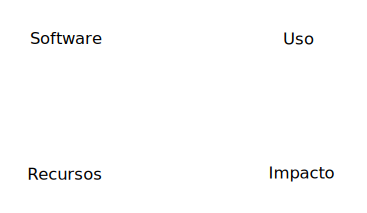
\includegraphics[scale=0.5]{imagens/process-model-scientific-software.png}
  \caption{A process model of software in science \cite{howison2015understanding}}
  \label{process-model-scientific-software}
\end{figure}

A Figura \ref{process-model-scientific-software} apresenta um diagrama deste
modelo de processo de softwares na ciência, este modelo é detalhado à seguir,
cada ator atua nos softwares, recursos, uso, impacto científico, detalhados à
seguir.

\subsection{Software}

Software acadêmico ({\it academic software}) é todo software usado para
coletar, processar ou analisar resultados de pesquisas com intenção de ser
publicados na literatura academica (seja num jornal, revista, conferência,
monografia, livro ou tese), podem ser desde protótipos escritos pelos próprios
cientistas, até mesmo produtos completos desenvolvidos profissionalmente
\cite{allen2017engineering}.

Podem ser encontrados na literatura acadêmica com outros nomes,
{\it research tool} \cite{Portillo12},
{\it research-originated software} \cite{Kon2011},
{\it research software} \cite{hettrick_2014_14809} ou
{\it scientific software} \cite{segal2008developing},
esses artefatos tem sido estudados dos mais variados pontos
de vista, desde de sua qualidade interna, até o impacto que
causam no meio científico.

No contexto de ecossistema de software acadêmico identificou-se cinco
motivações principais para a criação e contribuição ao software acadêmico:

\begin{enumerate}
  \item Ganho monetário direto (comercial software, employed software developers)
  \item Reputação acadêmica (incidental software, dirigido pela necessidade científica direta)
  \item Prática de software paralela (scientific needed enhanced by publishing 'software papers' alongside domain research)
  \item Um software de uma subárea de pesquisa (reputação direta pelo trabalho do software)
  \item Híbridos como licença-dual e 'software work' dentro de grandes colaborações (software como uma contribuição científica direta)
\end{enumerate}

\subsection{Recursos}

Os recursos investidos na produção destes softwares vem de diversas fontes,
incluem ganhos monetários diretos, recursos alocados em projetos, colaboração
entre laboratórios de pesquisa, e grande parte do ``tempo livre'' dos
pesquisadores em busca de soluções em suas pesquisas, este ``tempo livre''
perpassa por financiamentos diversos, carreira individual do cientista,
estudantes de graduação, prêmios, etc.

Independente da origem dos recursos o desenvolvimento de softwares acadêmicos
possui a particularidade de ser desenvolvido em sua grande maioria pelos
próprios cientistas uma vez que geralmente é necessário conhecimento no domínio
da pesquisa onde o software está inserido \cite{segal2008developing, hettrick_2014_14809,
momcheva2015software}.

\subsection{Uso}

% ... software é distribuido, utilizado e dá suporte à ciencia, gerando impacto ...

Estes artefatos de software são usados ativamente em diversos campos de pesquisa, como
matemática, biologia, física de partículas, astronomia, medicina e direito,
eles resolvem problemas comuns do cotidiano de pelo menos metade dos
pesquisadores de todas as áreas, desde grupos trabalhando exclusivamente com
problemas computacionais até grupos em laboratórios tradicionais ou em campo
\cite{wilson2014best}.

Os cientistas usuários finais mencionam tais softwares em suas publicações,
seja através de citação formal, informal, ou qualquer outro tipo de menção ao
software em suas pesquisas, estas citações ou menções fazem parte da economia
de reputação científica e causam impacto científico.

O impacto científico geralmente justifica o investimentos de novos recursos ao
ecossistema do software, seja para fins de planejamento, seja como
retrospectiva para avaliar os investimentos já realizados.

\subsection{Impacto científico}

% ... impacto científico justifica e potencialmente gera mais recurso ...
% \cite{katz2014transitive}

Ao longo da história, a citação formal tem sido utilizada para garantir
autenticação e autoridade, em vez de dar crédito e promover reconhecimento, na
história ocidental a citação aparece no final dos anos 1500, no início dos anos
1700 surge também no sistema legal, o ``copyright'' como reconhecendo aos
direitos autorais também surge nesse período, 1710.

A autoria das publicações tem sido realmente usado para reconhecer os autores e
contribuidores de um certo estudo, por exemplo, nos casos em que vários grupos
reivindicam crédito pelo mesmo avanço, ``backward citing'' tem sido utilizado
para verificar como as maiores comunidades de pesquisa atribuem crédito,
``forward citing'' também tem sido usada em casos onde se quer entender como
uma idéia foi usada após o seu surgimento ou publicação.

Conhecimento novo é claramente construído a partir do conhecimento passado.
Tradicionalmente, um autor cita um artigo anterior adicionando uma referência
ao autor, título, local de publicação, etc. No entanto, esse conceito não
funciona bem para produtos digitais como o software, que muitas vezes depende
de outros softwares, fragmentos de código, e algoritmos.

Este debate tem sido realizado a bastante tempo entre as diversas áreas da
bibliometria, cienciometria, altmetria e áreas similares, o fator de impacto
por exemplo proposto em 1955 apesar de continuar contribuindo para a ciência se
mostra muitas vezes utilizado da forma errada e mostra as deficiências de lidar
bem com produtos digitais gerados durante pesquisas.

\section{Sustentabilidade do ecossistema de software acadêmico}

% problemas identificados no ecossistema de software acadêmico

Um estudo sobre ecossistema de software acadêmico percebeu através dos relatos
de grande parte dos colaboradores participantes do estudo que os projetos de software
acadêmicos desenvolvidos na própria academia sofrem de {\it ``dysfunctional
chaotic churn''}, ou seja, a existência de muitos projetos, com poucos
usuários, com ciclos de vida curtos, que terminam em paralelo ao financiamento
inicial, comunidades desconectadas e paralelas, incompatibilidades entre
projetos, e tentativas aparentemente não coordenadas de ``reiniciar'' tudo
({\it re-boots}) \cite{howison2015understanding}.

Apesar de não haver evidências a respeito deste problema de forma tão abrangente,
sabe-se que parte dos problemas são realmente fato, por exemplo,
o {\it Dagstuhl Perspective Workshop}, evento organizado por um grupo de
pesquisadores sêniores de renome internacional, realizado anualmente na
universidade de Dagstuhl\footnote{\url{http://www.dagstuhl.de}} com o objetivo
refletir sobre o estado da ciência da computação explorando tópicos novos e
emergentes, em sua mais recente edição o workshop debateu sobre software
acadêmico e os problemas comuns em seu desenvolvimento, reconhecimento e
sustentabilidade \cite{allen2017engineering}.

\subsection{Desenvolvimento}

O desenvolvimento de software acadêmico ocorre em grande parte dentro da
própria academia, estudos mostram que pelo menos metade dos cientistas desenvolvem
seus próprios softwares, ao menos pacialmente, em domínios específicos este
número pode ser bem maior, na astronomia, por exemplo, estudos mostram que este
número pode chegar a 90\% \cite{hettrick_2014_14809, momcheva2015software}.

A grande participação dos cientistas no desenvolvimento destes artefatos de
software costuma ser um reflexo do tipo de conhecimento necessário ao se
desenvolver tais artefatos de software, pode ser necessário entender como o DNA
genômico se transforma em cristais de proteína, ou os meandros da dinâmica dos
fluidos, ou como resolver 20 equações diferenciais parciais simultâneas
\cite{segal2008developing}.

Desenvolvimento de software, exige algum conhecimento sobre o domínio, software
acadêmico não é diferente, mas esta grande participação dos cientistas no
desenvolvimento de software acadêmico começa a se tornar uma preocupação à
medida que a maior parte não possui treinamento algum sobre como escrever
softwares de forma eficiente, muitos não testam ou documentam os seus
softwares, faltam práticas básicas de desenvolvimento, como escrever código
legível, revisão de código, controle de versão, testes unitários, entre outros
\cite{wilson2017good}.

A qualidade dos softwares acadêmicos tem sido questionada,
a maioria também não sabe o quão confiável seu software é \cite{Merali2010Computational},
muitos estão em estado inicial de desenvolvimento \cite{marshall2013tools},
poucas foram testados fora do contexto onde foi desenvolvido \cite{Portillo12}.

Ocasionando sérios erros computacionais em conclusões centrais da literatura
acadêmica, gerando retrabalho para retratar tais erros nas mais diversas áreas
da ciência \cite{Merali2010Computational}. Dados são perdidos, análises levam
mais tempo que o necessário e os pesquisadores não conseguem a eficiência que
poderiam ter ao trabalhar com softwares acadêmicos \cite{wilson2017good}.
Causando um impacto negativo na visibilidade dos softwares acadêmicos
\cite{howison2013, katz2014transitive} e na capacidade de serem encontrados e
compartilhados.

\subsection{Reconhecimento}

% visibilidade

Apesar do crescimento no uso de software e na consequente dependência entre
cientistas de todos os campos, tornando o software acadêmico parte integral da
prática científica, apesar do apelo da comunidade científica para que o
software acadêmico seja tratado como cidadão de primeira classe, estudos tem
mostrado que muitas pesquisas não mencionam sequer o uso de software acadêmico
em suas publicações mesmo tendo feito uso de tais artefatos
\cite{momcheva2015software} \cite{howison2016software}.

Isto tem prejudicado a visibilidade do software acadêmico causando impacto
negativo em seu ecossistema, um software invisível é frequentemente excluído de
revisões por pares, uma atividade que costuma contribuir para a qualidade geral
do trabalho publicado, além disso, o
impacto negativo na visibilidade do software acadêmico faz surgir uma
série de questionamentos sobre a sua qualidade e também sobre a
capacidade de ser encontrado, compartilhado e co-desenvolvido
\cite{howison2013, katz2014transitive} \cite{howison2016software}.

Apesar de nem sempre ser possível, ou viável, ter tudo dentro de padrões
estritos, é preciso estar consciente das boas práticas ao produzir e utilizar
softwares acadêmicos, tanto para melhorar a própria abordagem quanto para
revisar outros trabalhos \cite{wilson2014best}.

Um software acadêmico em bom funcionamento devem atingir não apenas os
objetivos de entendimento e transparencia, mas também os objetivos voltados
para replicação \cite{Stodden2010}, seja logo após sua publicação, seja daqui
a 10 ou 50 anos.

\subsection{Sustentabilidade}

O desenvolvimento de software sustentável tem sido identificado como um desafio
chave no campo da ciência e da engenharia computacional, se sustentabilidade
não for levada em consideração em projetos de software, não importa qual o
domínio ou qual o propósito do software, perde-se a oportunidade de causar
mudanças positivas no planeta e na sociedade.

Apesar de sustentabilidade ser um conceito complexo e com mútiplas dimensões,
levando a debates profundos, o conceito geral é bastante simples e refe-se à
capacidade de perdurar e de continuar sendo suportado ao longo do tempo, isto
implica na qualidade de longevidade e manunetabilidade do software
\cite{venters2014software}.

Software sustentável é aquele que continua a estar disponível no futuro, em
novas plataformas, atendendo continuamente às novas necessidades do ambiente
... adequada evolução frente as condições do ambiente em constante mudança
\cite{allen2017engineering}.

Estudo mostra o decaimento das URLs ao longo do tempo, fundamenta o assunto,
mostra grafico com o caimento ao longo dos anos em publicações da
bioinformática, grafico muito bom cruzando e decaimento e tendencia com os
passar do tempo \cite{wren2017use}.

O {\it Journal of the American Statistical Association (JASA)} tem insistido na
necessiade de estarem disponíveis código e dados durante a revisão dos
manuscritos \cite{baker2016scientists}, Agências de financiamento como o {\it
US National Science Foundation} estão começando a reconhecer produtos de
pesquisa, como software, assim como fazem com as publicações, isto reconhece as
contribuições ao softwares assim como primeiro produto de pesquisa.

Isto visa especialmente garantir a longevidade dos artefatos e proporcionar que
um segundo pesquisador receba todos os benefícios do trabalho duro do primeiro
pesquisador \cite{king1995replication}, já que tanto a ciência quanto a
engenharia dependem de resultados incrementais para sua evolução. No terceiro
compromisso, relacionado ao conceito {\it desenvolvimento}, o Dagstuhl
Manifesto enfatiza a necessidade de medir a qualidade e a sustentabilidade dos
softwares científicos, tanto a priori quanto a posteriori.

\subsubsection{Manutenabilidade}

% falar de manutenabilidade como um eixo dentro de sustentabilidade técnica

A adoção e uso de softwares acadêmicos está relacionada, entre outros fatores,
também à sua qualidade, portanto é impoprtante medir e coletar sua qualidade de
alguma forma, qualidade é um vasto assunto, um dos problemas comuns enfrentado
pelos pesquisadores que desenvolvem tais softwares é a manutenabilidade
\cite{Prlic2012}.

Estudos tem mostrado que grande parte das ferramentas de software criadas na
academia estão em estado inicial de desenvolvimento \cite{marshall2013tools} e
que apenas uma pequena porcentagem são testados fora do contexto onde foi
desenvolvido \cite{Portillo12}.

%%%%%%%%%%%%%%%%%%%%%%%%%%%%%%%%%%%%%%%%%%%%%%%%%%%%%%%%%%%%%%%%%%%%%

%Cita um mapeamento feito sobre estudos que criam ferramentas para apoio a
%revisão sistemática no domínio de SE, 14 estudos foram selecionados, ao final
%apenas 8 tinham proposta de ferramentas, ao final conclui que as ferramentas
%encontradas estão em estado inicial de desenvolvimento \cite{marshall2013tools}.

%Cita um mapeamento sistemático com objetivo de encontrar ferramentas de
%comunicação e coordenação para suporte a times altamente distribuidos
%gograficamente, encontrou 132 ferramentas, para uso em projetos de software
%global. A maioria destas ferramentas foram desenvolvidas em centros de
%pesquisas, e apenas uma pequena porcentagem (18.9\%) foram testados fora do
%seu contexto onde foi desenvolvido \cite{Portillo12}.

%Computer systems research spans sub-disciplines that in-
%clude embedded and real-time systems, compilers, network-
%ing, and operating systems. Our contention is that a number
%of structural factors inhibit quality research. We highlight
%some of the factors we have encountered in our work and ob-
%served in published papers and propose solutions that could
%both increase the productivity of researchers and the quality
%of their output \cite{Vitek2011}.

%Além da aplicação, estes softwares variam também no papel que ocupam em suas
%pesquisas, alguns fazem parte dos resultados da pesquisa, como por exemplo,
%propostas de novos algoritmos ou técnicas de produção, outros são utilizados
%como parte do método de pesquisa, como coleta ou análise de dados, sendo que
%estes papeis não são excludentes.
%
%estes costumam ser citados pelos seus autores como uma das contribuições do
%estudo, seja principal ou secundária, 
%Esses softwares podem, de fato, ser um software de simulação complexo desenvolvido
%e executado em um computador de alto desempenho, mas também pode ser um
%software desenvolvido em um PC para incorporação em instrumentos; para
%manipular, analisar ou visualizar dados; ou para orquestrar fluxos de trabalho.

%e à medida
%que percebe-se que os softwares estão se tornando parte integrante dos
%processos, ferramentas e produção científicas, torna-se necessário e urgente
%discutir o seu desenvolvimento, visibilidade, qualidade e sustentabilidade.

% mostrar os beneficios da ciencia aberta, ciberinfraestrutura, etc
% * (favorecendo a ciencia e tornando a vida mais feliz para todos)

% mostrar os problemas para a ciência como um todo
% * causando problemas para o progresso de ciência, dados perdidos, etc, retrabalho
%   dificuldade de reprodução, etc...

%, não apenas técnica, mas também a
%capacidade de ser encontrado, compartilhado e co-desenvolvido, qualidades
%importantes para a evolução do próprio software, mas também extremamente útil
%para um uso eficiente dos limitados recursos da ciência \cite{howison2013,
%katz2014transitive}.

%contradizendo as boas
%práticas de qualquer projeto experimental, de ter {\it laboratory
%notebooks}\footnote{\url{https://en.wikipedia.org/wiki/Lab_notebook}}, dados
%organizados, passos documentados, e projeto estruturado para reprodutibilidade.

%softwares acadêmicos, assim
%como qualquer outro aparato experimental, são tão importantes para a ciência
%quanto são os telescópios ou tubos de ensaio \cite{wilson2014best}.

%Cientistas gastam mais tempo hoje utilizando e desenvolvendo softwares do que
%gastavam no passado.

%Software is a critical part of modern research and yet there is little support across the
%scholarly ecosystem for its acknowledgement and citation. Inspired by the activities
%of the FORCE11 working group focused on data citation, this document
%summarizes the recommendations of the FORCE11 Software Citation Working
%Group and its activities between June 2015 and April 2016. Based on a review of
%existing community practices, the goal of the working group was to produce a
%consolidated set of citation principles that may encourage broad adoption of a
%consistent policy for software citation across disciplines and venues. Our work is
%presented here as a set of software citation principles, a discussion of the motivations
%for developing the principles, reviews of existing community practice, and a
%discussion of the requirements these principles would place upon different
%stakeholders. Working examples and possible technical solutions for how these
%principles can be implemented will be discussed in a separate paper.
%\cite{smith2016software}

%Improving academic software engineering projects: A comparative study of academic and industry projects
%(compara as praticas de desenvolvimento da industria e academia e sugere melhorias, 1998!)
%https://link.springer.com/article/10.1023%2FA%3A1018925902814?LI=true

% papel pesquisador no ecossistema de soft academico
%
%Essas preocupações gerais sugerem um conjunto de questões específicas, com foco
%em padrões globais e padrões emergentes dentro do ecossistema, incluindo: Quais
%recursos foram destinados à produção de software? Quantos usuários ou
%comunidades de usuários têm projetos? Quais são os impactos científicos desse
%uso? Os números de usuários crescem? Os projetos possuem recursos e habilidades
%suficientes para gerenciar seu crescimento? Quais projetos possuem
%funcionalidades sobrepostas? Há quanto tempo os pedaços de software e projetos
%persistem? Nós desconectamos as comunidades de usuários e desenvolvedores? São
%componentes específicos, ou camadas de componentes, faltam? Que código
%geralmente é usado em conjunto; são os projetos e as pessoas que produzem esses
%componentes se comunicando adequadamente? Como podemos sustentar o software
%crítico?
%
%Aqui há uma clara tensão entre um desejo de flexibilidade e liberdade, ligado
%às expectativas de inovação científica e desejos de estruturas de autoridade e
%controle de coordenação. As questões de influência incluem: como os programas
%de financiamento e quais os requisitos em suas chamadas, resultaram em software
%amplamente utilizado e impacto científico substancial? Quais são as
%características dos campos que alcançaram maior coalescência? Quais jornais e
%conferências têm políticas exemplares? Como o trabalho de software é visto
%dentro das práticas de contratação e avaliação, como os casos de posse?
%
%\cite{howison2015understanding}

%Ao longo da história, a citação formal foi para autenticação e autoridade, em
%vez de de crédito e reconhecimento ou atribuição. A  científico citação na
%história ocidental aparece no final dos anos 1500. No início dos anos 1700, a
%citação também aparece no sistema legal como método de compreensão dos
%precedentes \cite{katz2014transitive}.

%A ideia de direitos autorais como reconhecendo aos direitos dos seus autores
%também surge nesse tempo, 1710, talvez devido a uma lenta tendência social
%societária de reconhecer a propriedade intelectual, uma idéia que parece ter se
%desenvolvido ao lado da imprensa]. Observe que a autoria de papers é realmente
%usado para notar os autores reais do artigo quanto para notar os contribuidores
%do projeto.
%Para muitos desses, o
%identificador que deve ser citado - um "nome" que se refere a um produto único
%não é claro.

%Additionally, if a cited library depends
%on another library, the contribution of this second library
%is not captured. Citation of a dataset should perhaps give
%credit to the people who gathered the data, as well as
%those who curated it, but the paper author may not know
%or be able to find these details.

%Mas independente de como seja calculado o impacto científico de uma determinada
%pesquisa o impacto causado se reverte potencialmente em mais recursos que
%poderão ser reinvestidos no próprio ecossistema onde o software está inserido.

%Science Code Manifesto \cite{barnes2013science}.
%Foco em código fonte escrito especificamente para processar dados de
%publicações, afirma que ``todo código fonte escrito especificamente para
%processar dados de uma publicação deve estar disponível para os revisores e
%leitores do paper''.

%Sustentabilidade é um conceito guarda chuva composto de múltiplas dimensões, em
%sua dimensão técnica, chamada sustentabilidade técnica, temos a preocupação com
%a longevidade da informação, dos sistemas, e infraestrutura, e sua adequada
%evolução frente as condições do ambiente em constante mudança.

%citações formais facilitam e promovem o avanço
%da ciência, mesmo diante da falta de um padrão para citar artefatos digitais
%\cite{allen2014credit}.

%Um estudo recente com 90 artigos de diversas áreas da biologia, selecionados
%aleatoriamente entre publicações usando softwares como método, mostrou que
%apenas 59 mencionavam o uso de softwares de alguma forma, os demais 31 artigos,
%apesar de usar software acadêmico, não mencionavam nada a respeito
%\cite{howison2016software}, apenas entre 31\% e 43\% das menções aos softwares
%acadêmicos envolvem citação formal.

%Não existe ainda amadurecimento suficiente sobre como citar softwares e
%outros artefatos digitais em pesquisas científicas, não temos um padrão de como fazê-lo,
%cada autor cita à sua maneira, muitas vezes ao longo do texto, outras em seções
%específicas sobre a implementação do software, nem semprem informam onde
%encontrar uma cópia do software, ou ainda nem sobre o modelo em que o software
%é distribuído, ou se é de alguma forma distribuído ao público.

%Entre os softwares acadêmicos desenvolvidos por cientistas como apoio em suas
%pesquisas, não é raro que pesquisadores deixem de disponibilizar estes artefatos,
%assim como outros desdobramentos da pesquisa, como dados e outros. Ou ainda,
%mesmo disponibilizando tais artefatos em locais de público acesso, com o tempo,
%tais locais se tornam indisponíveis inviabilizando a obtenção de tais
%artefatos.

%A comunidade tem refletido sobre os problemas relacionados ao
%desenvolvimento, promoção e sustentabilidade desses softwares, e o
%impacto que tais problemas causam no meio científico \cite{allen2017engineering}.

%, e faz
%surgir questionamentos sobre sua qualidade, não apenas técnica, mas também a
%capacidade de ser encontrado, compartilhado e co-desenvolvido, qualidades
%importantes para a evolução do próprio software, mas também extremamente úteis
%para o uso eficiente dos limitados recursos da ciência \cite{howison2013,
%katz2014transitive}.

\section{Ecossistema de software acadêmico de análise estática} \label{analise-estatica}

Ao falarmos sobre ecossistema de software acadêmico estamos nos referindo a
qualquer software, de qualquer domínio de aplicação, que tenha sido utilizado
ou produzido durante trabalhos de pesquisa com intuito de publicação na
literatura acadêmica.
%REVER - intuito de apoiar pesquisa que será eventualmente divulgada por meio da  publicação de resultados.

O ecossistema de software acadêmico de análise estática é um recorte deste
conjunto, a princípio, com as mesmas características, atores e modelo de
funcionamento, mas logicamente podendo apresentar particularidades trazidas
pela natureza do domínio de análise estática e suas ferramentas, soluções e
algoritmos.

\subsection{Análise estática}

A análise estática de código fonte é o primeiro passo para coletar informações
necessárias em diversas atividades de verificação, medição e melhoria da
qualidade de produtos de software \cite{cruz2009code, kirkov2010source}. Ela é
realizada com base no código fonte de um programa ou sistema de software, e a
partir daí descobre problemas e propriedades de sua qualidade estrutural
\cite{chess2007secure}.

Ferramentas de análise estática estão disponíveis há décadas, em especial,
para programadores. A ferramenta Lint \cite{johnson1978lint}, considerada a
primeira ferramenta de análise estática \cite{gosain2015static}, foi criada para
examinar programas escritos em linguagem C e aplicar regras de tipagem mais
estritas do que as regras dos próprios compiladores da linguagem.

Análise estática de código fonte tem como objetivo prover
informações acerca de um programa a partir do seu código fonte sem
necessidade de execução, e sem requerer qualquer outro artefato do programa
além do próprio código.

É um ramo que possui muitas das suas abordagens em comum com os estudos da
área de análise de programas ({\it program analysis}), especialmente na área de
compiladores, onde atua especialmente nas primeiras etapas do processo de compilação.

A análise estática de código fonte é considerada uma atividade meio com
objetivo de suportar uma variedade de tarefas comuns da engenharia de
software; muitas dessas tarefas são substancialmente úteis em atividades de
manutenção, incluindo \cite{binkley2007source}:

\begin{multicols}{2}
  \begin{itemize}
    \item Análise de performance
    \item Compreensão de programas
    \item Desenvolvimento baseado em modelos
    \item Detecção de clones
    \item Evolução de software
    \item Garantia de qualidade
    \item Localizaçao de falhas
    \item Manutenção de software
    \item Recuperação arquitetural
    \item Testes
  \end{itemize}
\end{multicols}

Seja em qual atividade for, a análise estática possui importância,
pois ao ser capaz de extrair informações diretamente do
código fonte de um programa, pode auxiliar a responder perguntas necessárias
para as diversas atividades de desenvolvimento e evolução de software. Essa
importância se torna ainda mais aparente diante da ``lei'' da tendência para
execução \cite{harman2010why} que indica que todos os tipos de notação tem a
tendência de se tornar executáveis.

% \subsection{Usos da análise estática de código fonte} \label{usos}

A análise de programas trata, de modo geral, da descoberta de problemas e
fatos sobre programas. Tal análise pode ser realizada sem a necessidade de executar o
programa (análise estática) ou com informações provenientes de sua execução
(análise dinâmica).

A ideia de que programas de computador podem ser utilizados para analisar
código fonte de outros programas tem uma história de mais de 40 anos.  O
programa PFORT \cite{ryder1974pfort} foi projetado para localizar potenciais
problemas na portabilidade de código Fortran; em função da diversidade de
dialetos de Fortran, uma compilação sem erros não indicava que o programa
estava correto segundo os padrões da linguagem \cite{wichmann1995industrial}.

Desde então, ferramentas de análise estática de código fonte têm surgido para
os mais diversos fins -- muitas delas a partir das pesquisas e
desenvolvimentos da área de compiladores.  O {\it parser} utilizado nessas
ferramentas têm funcionalidades análogas aos analisadores usados em
compiladores \cite{anderson2008the}.

O uso de tais ferramentas tem se tornado mais comum no ciclo de desenvolvimento de
software, sendo aplicadas em atividades distintas.
O campo de aplicação destas ferramentas é bastante variado, cobrindo diferentes
objetivos.

\subsection{Software de análise estática}

A variedade de aplicação e a constante evolução da área de análise estática, 
tanto na indústria quando na academia, resulta em  estudos teóricos e práticos, novas ferramentas, modelos e
algoritmos de análise estática. Ferramentas de análise estática têm sido
continuamente desenvolvidas e seu uso se tornado comum no ciclo de desenvolvimento de
software.

Mas apesar da rápida e constante evolução da área, ainda há carência de estudos
avaliando estas ferramentas \cite{li2010comparative}, mesmo com os avanços e com
ferramentas de sucesso, o desenvolvimento de análise estática ainda é conhecido
por ser um processo doloroso \cite{toman2017taming}.

A eficiência, confiabilidade e precisão dessas ferramentas têm sido avaliadas e
alguns estudos mostram inconsistência entre ferramentas diferentes.
Um estudo que comparou duas ferramentas de análise estática para cálculo de métricas,
revelou significantes evidências sobre a inconsistencia entre valores de métricas,
grande diferença nos valores, e discutiu quais problemas e questões levam a estas
diferenças \cite{alemerien2013experimental}.

Análise estática é a técnica mais amplamente utilizada para análise
automatizada de programas devido a sua eficiência, boa cobertura e automação.
Estudos mostram que analise estática tem grande adoção em projetos de software
livre \cite{beller2016analyzing}.
Entretanto,tecnicas de analise estatica amplamente adotadas na comunidade de software,
por exemplo, para localização de bugs e verificação de programas 
ainda sofrem um alto índice de falso-positivos \cite{gosain2015static}.

Apesar da ampla adoção de ferramentas de análise estática em estudos
acadêmicos e da crescente atenção que as técnicas de análise estática de código tem
recebido em pesquisas, nota-se ainda uma enorme distância entre a atenção dada na academia e sua adoção na indústria,
identificando um gap entre estes dois contextos \cite{ilyas2016static}.

\subsection{Software acadêmico de análise estática}

Em Ciência da Computação, particularmente em Engenharia de Software, tem-se
notado um aumento constante no número de novos softwares acadêmicos \cite{allen2017engineering},
especialmente em estudos de análise estática, 
uma área com uma longa e respeitável tradição em
pesquisas sobre a criação de novas ferramentas, métodos e algoritmos.

%Na indústria também a adoção de software de análise estática é crescente...

O software acadêmico de análise estática e o seu ecossistema, ao estar inserido
no sistema acadêmico e intimamente relacionado a economia de reputação
científica, sofre as consequências da competição que permeia este modelo, e o
seu uso invariavelmente deixa de gerar feedback positivo de volta ao seu ecossistema,
conforme Figura \ref{scientific-reputation-diagram}, onde se apresenta o
relacionamento entre a prática e a pesquisa de software acadêmico.

%está inserido no contexto similar
%a qualquer outro software acadêmico, e o seu ecossistema possui as mesmas
%características do ecossistema de software acadêmico, 

\begin{figure}[h]
  \center
  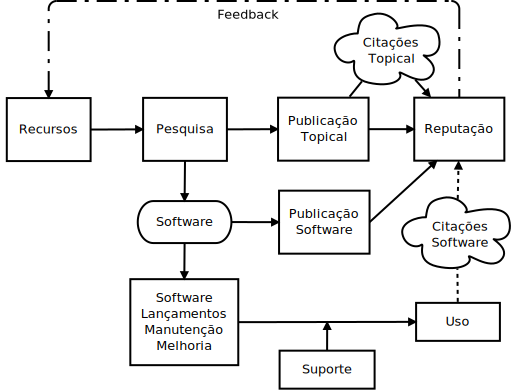
\includegraphics[scale=0.5]{imagens/scientific-reputation-diagram.png}
  \caption{Uma visão dos incentivos de reputação num contexto misto entre Ciência e práticas de software acadêmico \cite{howison2011scientific}}
  \label{scientific-reputation-diagram}
\end{figure}

%ecossistema de software acadêmico está inserido num contexto de competição

Diferentemente de outras tecnologias, software pode ser copiado e distriduído
essencialmente sem custo, abrindo portas sem precedentes em nível para
compartilhamento e inovação colaborativa \cite{howison2011scientific}, no
entanto, ao estar de alguma forma conectado ao contexto de competição da economia de
reputação científica, como no mecanismo de crédito acadêmico aos artigos e publicações,
pode ser potencialmente problemático para a colaboração e manutenção
\cite{howison2011scientific}.

%No entanto tem se percebido que o ecossistema de software acadêmico tem perdido
%oportunidade de colaboração visto que estão inseridos neste contexto ....
%competição, muitos softwares utilizados em pesquisas não são mencionados pelos
%seus autores causando impacto negativo em sua visibilidade, reconhecimento e
%consequentemente ...  \cite{howison2016software}.

Este cenário, além de desacelerar o progresso geral da Ciência gerando
retrabalho, faz surgir questionamentos sobre as conclusões dessas pesquisas,
especialmente quando grande parte dos pesquisadores não sabem o quão confiável
seus projetos de software são. Criando assim, um contexto em que muitos estudos
em Engenharia de Software sofrem de dificuldades de repetição
\cite{tang2016worthiness}, além de ocasionar problemas específicos relacionados a
manutenabilidade e sustentabilidade técnica do software acadêmico.

%Esta reflexão tem mostrado,
%por exemplo, 

%Junto com estas questões estão as questões de como
%influenciar o ecossistema, incluindo questões de pontos de inflexão que levam
%ao uso coalescente, bem como a intervenções políticas diretas incentivando o
%uso de componentes específicos.

%%%%%%%%%%%%%%%%%%%%%%%%%%%%%%%%%%%%%%%%%%%%%%%%%%%%%%%%%%%%%%

%While some of these seem relatively unproblematic, such as commercial
%production in fields with immediately valuable applications, others appear
%problematic. In particular we highlighted the potentially pernicious
%implications of the academic credit production system for collaboration and
%maintenance 

%Adicionalmente as relacões entre os atores do ecosistema como um todo
%são de mútuo interesse (mutualismo):

%O relacionamento entre os atores em um ecossistema de software, por outro lado,
%são caracterizados pela alto espectro de relacionamentos simbioticos.

%Dependendo dos atores e suas atividades, dois atores podem ter benefícios
%mútuos (mutualismo), estar em competição direta (competition/antagonism),
%estarem não afetados (neutralism) ou um não afetado enquanto o outro é
%beneficiado (amensalism) ou prejudicado (parasitism) por seu relacionamento

%em pesquisas sobre análise de código, ferramentas de analise estatica tem
%recebido significante mais atencao que outras tecnicas, tecnicas com formal e
%bem definidos processos recebem mais atencao de pesquisa e escrutinio porque
%estudos irao avaliar seu processo e elementos, entretanto, isto nao
%necessariamente significa que tecnica é melhor; The survey concluded that 1)
%the adoption of static code analysis techniques in the industry is influenced
%by the software life cycle model, while software product type and company size
%doesn’t have an influence. 2) The amount of attention a static code analysis
%technique has received in research doesn’t necessarily influence its adoption
%in industry indicating a gap between research and industry 3) company size,
%product type, and life cycle model do influence professionals perception on
%benefits/limitations.  \cite{ilyas2016static}

\section{Ciência e colaboração}

\subsection{Reprodutibilidade}

Enquanto pesquisadores publicam artigos descrevendo e divulgando seus
resultados, é raro que façam o mesmo com toda a produção gerada durante a
pesquisa. A maioria dos componentes necessários para a reprodução dos
resultados de uma pesquisa -- por exemplo, códigos fonte e dados -- usualmente
permanecem não publicados. Esse problema fere um dos fundamentos
da ciência de que novas descobertas sejam reproduzidas antes de serem
consideradas parte da base de conhecimento \cite{Stodden2009}.

%Nesse sentido, \citeonline{Prlic2012} enfatizam que disponibilizar o código
%criado durante pesquisas não apenas aumenta o impacto como também se torna
%essencial para outros reproduzirem os resultados encontrados, citam ainda que
%manutenabilidade e disponibilidade do software após a publicação é o maior
%problema enfrentado pelos pesquisadores que desenvolvem tais softwares.
%
%A replicação desses estudos empíricos pode, e deve, ser realizado, de modo a
%averiguar a validade e aumentar o nível de confiança em seus resultados,
%replicação costuma ser citado como um importante meio para validar estudos
%empíricos e assim aumentar o nível de confiança em seus resultados
%\cite{Almqvist2006}. A reprodução dos resultados de pesquisas aumenta o impacto
%social das pesquisas e gera economia de tempo e dinheiro para os pesquisadores
%e para as instituições \cite{Nesta2010}.

Apesar da preocupação com a reprodutibilidade dos resultados de pesquisas de
forma independente \cite{Stodden2009} e aberta, esta área tem recebido ainda
pouca atenção da comunidade de pesquisa \cite{Nancy2015, Grand2010Open}. Em um
estudo recente, com 88 papers do MSR entre 2004-2011, evidenticou-se que apenas
62\% são replicaveis ou parcialmente replicaveis e que apenas 20\% dos estudos
disponibilizam suas ferramentas \cite{amann2015software}. Um estudo anterior
com 171 papers do MSR evidenciam que, entre outros problemas, a maioria não
disponibilizam publicamente as ferramentas e scripts, mesmo quando os autores
explicitamente afirmam que construíram algum \cite{robles2010replicating},
apenas 2 entre 154 estudos experimentais avaliados fornecem os dados e as
ferramentas necessárias para replicação e futuras pesquisas
\cite{barr2010shoulders}.

Reprodutibilidade ({\it reproducibility}) é a habilidade de replicar um experimento
ou estudo em sua totalidade a fim de confirmar suas hipóteses, seja pelo
autor ou por pesquisadores independentes. Esse conceito é um ponto
central do método científico e continua a receber bastante atenção ainda hoje,
como pode ser verificado em estudos recentes.

\citeonline{Stodden2009} preocupada com as barreiras legais para
disponibilidade de artefatos de pesquisa propõe o framework ``{\it Reproducible
Research Standard (RRS)}'', onde sugere formas de usar o licenciamento e as leis
de copyright da melhor forma para manter disponíveis os produtos gerados
durante pesquisas e assim viabilizar reprodutibilidade. \citeonline{Vitek2011}
em um estudo sobre reprodutibilidade e rigor científico destacam a importancia
de se disponibilizar qualquer material suplementar gerado durante uma pesquisa
de modo a possibilitar revisores verificarem e replicarem experimentos. Em
2012, um workshop intitulado ``{\it Reproducible Research: Tools and Strategies for
Scientific Computing}'' \cite{Stodden2012} discutiu, especificamente, iniciativas
e ferramentas voltadas a apoiar pesquisas reprodutíveis.
\citeonline{Krishnamurthi2015}, em um estudo sobre repetibilidade, chamam
atenção para o papel central que os artefatos de software possuem em pesquisas
de ciência da computação e questionam: "Onde está o software nas pesquisas
sobre linguagem de programação?". \citeonline{Stodden2015} demonstram o
projeto "ResearchCompendia.org", uma infraestrtura para reprodutibilidade e
colaboração em ciência computacional. Além destes e tantos outros estudos em
\cite{GithubReproducibilityGuide} é possível acessar um guia sobre como
desenvolver pesquisas cientíticas de forma que promovam a reprodutibilidade.

Apesar do termo reprodutibilidade ser relativamente concensual entre as várias
áreas da ciência, existem alguns termos relacionados com uma certa diferença
de significado, diante disto, e preocupado em criar uma linguagem comum entre
os pesquisadores, \citeonline{Feitelson2015} propôs as seguintes definições:

\begin{description}

  \item[Repetição (repetition)]
  Refazer exatamente o que outra pessoa fez usando os artefatos originais.

  \item[Replicação (replication)]
  Replicar com precisão exatamente o que outra pessoa fez, recriando os
  artefatos.

  \item[Variação (variation)]
  Repetir ou replicar exatamente o que a outra pessoa fez, mas com alguma
  modificação controlada nos parâmetros.

  \item[Reprodução (reproduction)]
  Recriar o espírito do que outra pessoa fez, usando seus próprios artefatos.

  \item[Corroboração (corroboration)]
  Obter os mesmos resultados de outra pessoa, usando outros meios e
  procedimentos experimentais.

\end{description}

É conhecido que a ciência precisa de reprodutibilidade e corroboração para
realmente fazer progressos, mas a prática de forma abrangente ainda é um
obstáculo. Diante disso \citeonline{Peng2011} sugere adotar soluções
intermediárias, repetição, replicação, variação, e desta forma já teríamos uma
grande melhoria sobre a situação atual onde muitos estudos em engenharia de
software sofrem de dificuldades de repetição \cite{Tang2016} e,
consequentemente, poucos estudos replicando pesquisas da área são encontrados
\cite{da2011replication}.

Mesmo sabendo que todo artefato tem impacto na reprodutibilidade
\cite{gonzalez2012reproducibility}, uma barreira comum para tal prática, e
consequentemente para repetição, replicação e variação é a indisponibilidade do
código fonte. Toda pesquisa que possua qualquer processo computadorizado deve
publicar seus códigos, eles precisam estar disponíveis, mesmo que os dados
correspondentes não estejam, o código deve estar. De acordo com o espectro de
reprodutibilidade (Figura \ref{reproducibility-spectrum}), a disponibilidade de
código é o requisito mínimo e é o primeiro passo para possibilitar validação e
confirmação dos resultados.

\begin{figure}[h]
  \center
  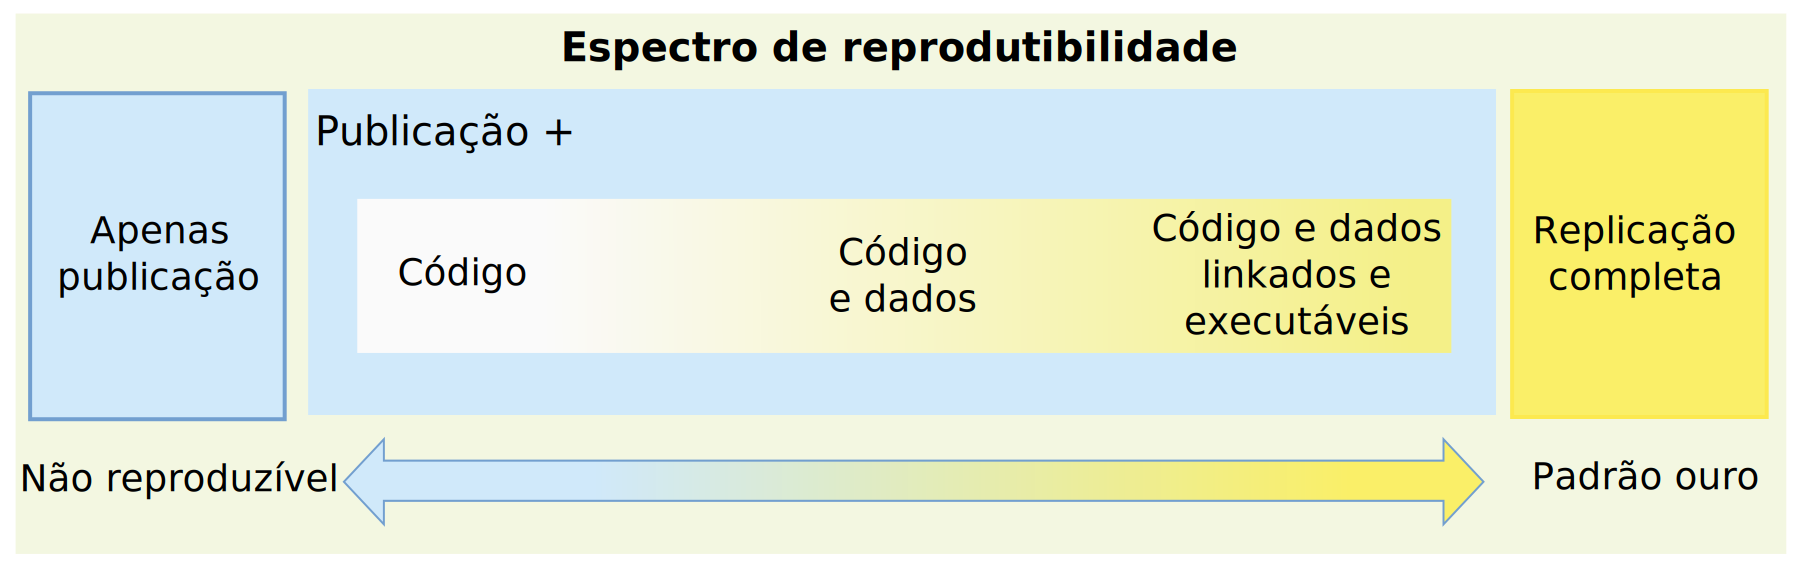
\includegraphics[scale=0.35]{imagens/reproducibility-spectrum-ptbr.png}
  \caption{Espectro de reprodutibilidade \cite{Peng2011}}
  \label{reproducibility-spectrum}
\end{figure}

Apesar das pesquisas reproduzíveis ({\it RR - Reproducible Research}) não
resolverem todos os problemas de validade experimental dos estudos em
engenharia de software, elas ao menos garantem que dados e métodos de análise
estejam disponíveis para inspeção e que os resultados possam ser derivados,
facilitando revisão logo que a publicação acontece. Além disso, é um recurso
valoroso para pesquisadores iniciantes, pesquisas reproduzíveis melhoram o
impacto do próprio estudo, por exemplo, artigos de computação que não
disponibilizam pubicamente dados e códigos possuem menos chances de serem
citados \cite{madeyski2017would}.

\subsection{Ciência aberta}

Ciência Aberta é um movimento que tem por objetivo tornar a pesquisa
científica, seus dados e sua disseminação acessíveis à todos os interessados,
sejam amadores ou profissionais \cite{WikipediaOpenScience}. Sua principal
motivação está em possibilitar a reprodução dos resultados de pesquisas e em
garantir transparência das metodologias utilizadas, isto aumenta o impacto
social das pesquisas e gera economia de tempo e dinheiro para os pesquisadores
e para as instituições \cite{Nesta2010}.

Este movimento é guiado por princípios básicos de transparência, acessibilidade
e reusabilidade universais, disseminadas via ferramentas online, ele é dividido
em quatro grandes áreas: (1) Open Access, (2) Open Data, (3) Open Source e (4)
Open Reproducible Research. Dentre elas destaca-se a Open Reproducible Research
por preocupar-se com a reprodutibilidade dos resultados de pesquisas de forma
independente \cite{Stodden2009} e aberta, no entanto, esta área tem recebido
ainda pouca atenção da comunidade de pesquisa \cite{Nancy2015}
\cite{Grand2010Open} apesar do aumento geral do interesse pelas práticas da
Ciência Aberta \cite{Grand2010}.

%Over the past fifteen years the scholarly communications agenda
%has progressed gradually. Currently we are experiencing a strong
%tendency among all research stakeholders to engage with the
%practice of OS. Lately, research funders require the sharing not
%only of the research results they have funded, but also of the
%procedures and data that are being generated during the research
%conduct. Researchers, on the other side, are keen on observing
%their research results being used for the improvement of the
%society and are forced by their funders to demonstrate the impact
%of their research. At the same time, higher academic institutions
%aim to join the OS agenda as well, since they see the opportunity
%of great economic benefits and savings. While OS is the possible
%answer to all these factors, the stakeholders’ inability to
%understand the requirements for the application of OS can be a
%suspensory factor for the OS implementation and evolution.
%The aim of the FOSTER project is to advance the stakeholders'
%knowledge on the usefulness of OS and explain the technicalities,
%strategies and best practices using which OS can be applied. As an
%attempt to educate the largest number of researchers possible,
%FOSTER has created an e-leanring portal, which contains quality
%assured information relating to the topic and it is open to everyone
%in the world. The platform contains two types of information:
%learning material and online courses. The classification of these
%two types is supported by an OS taxonomy, where related terms
%are applied both in the portal's material and also in the courses.
%With the use of the taxonomy, users are in the position to
%understand the OS domain and the concepts around it.
%The main goal of the FOSTER project, which is mainly achieved
%through the portal functionalities, is not only to educate the
%research stakeholders on OS, but also to build a community of
%researchers, librarians, software developers, funders and research
%administrators who are interested in OS in order to advance the
%way research is being conducted and shared. In addition, FOSTER
%attempts to provide tools to this community, such as re-usable
%content for training and a platform for blended learning and e-
%learning courses that the community could run. This OS
%advancement is essential for the research promotion and,
%consequently, for the benefit of the society as a whole
%\cite{Nancy2015}.
%
%Open Science may be practised both
%for philosophical and pragmatic reasons. As the
%resources produced by open projects are
%potentially accessible to public audiences, Open
%Science offers both a novel medium for public
%access and involvement in the process of science
%and an innovative method for real-time science
%communication. Does such direct access clear
%the stream of communication or muddy the
%waters with unfocussed, unclear and unvetted
%comment? This paper suggests that adopting an
%Open Science approach allows the capture of an
%authentic and clear record of research.
%However, researchers acknowledge this involves
%opening their work up to a different type of
%scrutiny \cite{Grand2010}.
%
%Open Science is an emerging approach to the conduct of science, technology and engineering
%projects, in which information about the whole of an ongoing investigation is made available
%on and through the Internet. Adopting an Open Science approach means the audience for the
%research can extend beyond the researchers involved to other researchers and to members of
%the public. Thus, Open Science has implications for engineering research, practice,
%publishing and public engagement with engineering. This paper reviews the history and
%evolution of the Open Science movement, includes some reflections on the related areas of
%Open Access, peer-review and public engagement with science and engineering and discusses
%data gathered from interviews. The analysis suggests that interviewees have concerns about
%issues such as precedence and protection of original work and the time needed to integrate
%open science practices into daily work. Successfully working in such collaborations is likely
%to require not only common practical tools but also the development of shared language and
%understanding between researchers and members of the public. Interviewees recognise the
%value of Open Science in collaborative research and its innovative facility to sustain direct
%public access to research outputs. It also has the potential to allow members of the public to
%make real practical contributions to research \cite{Grand2010Open}.
%
%This white paper was written as a contribution to the “Imagining
%Tomorrow’s University: Rethinking scholarship, education, and institu-
%tions for an open, networked era” workshop, a joint NIH/NSF-funded
%event held 8–9 March 2017 in Rosemont, IL. In this paper, I present an
%overview of what I consider open science, its importance, and how it
%plays a role in my research agenda. I also discuss challenges faced in
%pursuing research openness, and recommend changes to university
%leaders to address these barriers \cite{niemeyer2017open}.
%
%Open to All?  Case studies of openness in research
%Since the early 1990s, the open access movement has promoted the concept of openness in relation
%to scientific research. Focusing initially upon the records of science in the form of the text of articles
%in scholarly journals, interest has broadened in the last decade to include a much wider range of
%materials produced by researchers. At the same time, concepts of openness and access have also
%developed to include various kinds of use, by machines as well as humans.
%Academic bodies, including funders and groups of researchers, have set out statements in support
%of various levels of openness in research. Such statements often focus upon two key dimensions:
%what is made open, and how; and to whom is it made open, and under what conditions? This study
%set out to consider the practice of six research groups from a range of disciplines in order to better
%understand how principles of openness are translated into practice \cite{Nesta2010}.

\subsection{Ciberinfraestrutura}

A visão da ciberinfraestrutura, expressada no "Relatório Atkins" e instanciada
para o ecossistema de software científico na NSF chamada de Infraestrutura de
Software para Inovação Sustentada (NSF SI2),

Os softwares vem não apenas atuando no avanço da ciência, mas atuando com uma
eficiência crescente ao longo do tempo (Atkins 2003). A chave para isso é a
crença de que o software deve evoluir em direção a uma plataforma
compartilhada, com componentes que são reutilizados o mais amplamente possível,
já que os usuários finais e os produtores de componentes se agrupam em torno de
peças específicas de software.

a literatura sobre plataformas de software fora da ciencia tem chamado isso de
'coring' e 'tipping' (Gawer and Cusumano 2008),
onde uma comunidade descobre sua funcionalidade compartilhada e se agrupa
em pacotes que fornecem, levando ao uso eficiente de recursos através de
economias de escala.

coring também resulta em um aumento do uso sobreposto que facilita mais

Isto também resulta em um aumento do uso sobreposto que facilita mais
transparência na ciência, levando a uma maior qualidade e correctude (correctness), à medida
que mais olhos e esforços são direcionados para os mesmos códigos que são
sustentados e evoluem em longos períodos de utilidade científica.

coring em direção às plataformas pode ser contrastado com o seu oposto, muitas
vezes percebido por informantes: churn caótico disfuncional, com muitos
projetos com poucos usuários, cada um tendo vidas curtas que terminam com o
financiamento de concessão inicial, comunidades desconectadas e paralelas,
incompatibilidades teimosamente imutáveis e periódicas e tentativas
aparentemente não coordenadas de "reiniciar". Subjacente a isso é uma
preocupação que as oportunidades são perdidas e que o progresso da ciência é
abrandado (por exemplo, Stewart, Almes e Wheeler 2010).


%%%%%%%%%%%%%%%%%

O ecosistema de software acadêmico é um sistema que consome tempo, dinheiro e
atençao, e afeta a conduta e os resultados da ciência, tanto no geral, como em
campos específicos

chape para isto é acreditar que software deve evoluir para plataformas compartilhadas,
com componentes reusáveis tanto quanto possível, tanto para usuário final, quanto
para produtores de componentes (papel) agregando peças particulares de software


% fez exatamente o que pensei, vou ler para usar a metodologia "adaptada"
%In addition to these motivation studies, scientists have recently embarked on the issue of
%software use and impact. A study in 2013 has found that scientists tend to choose software
%that is widely used by others in their community and prefer software that is free for
%academic use (Huang et al. 2013). Studies on the scientific software ecosystem have
%suggested that the use of scientific software is influenced by its visibility, availability,
%sustainability, reproducibility, and citation (Howison and Herbsleb 2014; Howison et al.
%2015; Huang et al. 2013). Studies also have suggested that software developers are
%interested to know the use and impact of their software because ‘‘software use matters to
%them for funding purposes’’ (Howison et al. 2015; Trainer et al. 2015, p. 428).
%Recent studies on data impact have led to the discussions on software citation and
%evaluation, as a parallel can be drawn between software and data in scientific literature
%(Piwowar et al. 2011; Howison and Bullard 2016). It is suggested that the numbers of
%mentions and citations in literature can be used to measure the impact of software (Huang
%et al. 2013; Pan et al. 2015). Yet, it is argued that ‘‘the practices of citation to software vary
%considerably from field to field and appear to miss significant software’’ (Howison et al.
%2015, p. 478). One study examining the use of software in scientific articles in biology has
%found that more than half of the software mentions did not include references (Howison
%and Bullard 2016). Thus, it validates the need to use alternative metrics in addition to
%citations when assessing software impact, such as the numbers of downloads, registered
%users, subscribers, user reviews, and artifacts inserted in literature (Howison et al. 2015).

Assim, surge um conjunto de ações que podem ser tomadas pelos diferentes atores
em direção à garantir sustentabilidade nos projetos de software, ações para
praticantes de software, pesquisadores, associações profissionais, educadores,
cientes e usuários.

Inevitavelmente alguns softwares irão continuar sendo úteis após o primeiro
release, alguns terão algums gerações de melhorias, outros serão usados na sua
versão original sem atualização ou manutenção, e alguns outros irão ser
lançados e nunca utilizados. Isto é perfeitamente natural, a comunidade ao
redor do software irá decidir qual é o melhor caminho a se tomar num processo
evolutivo \cite{weiner2009astronomical}.

lugar, em algum momento. Uma utilidade óbvia para qualquer um destes softwares
é para aqueles que desejam replicar as pesquisas em que foram criados, seja com
o simples objetivo de validar as conclusões, seja com interesse de estender e
colaborar com a pesquisa original.

... para garantir a reprodutibilidade dos seus estudos.


\subsection{Pesquisas reproduzíveis}


% Software Carpentry: lessons learned [version 2; referees: 3 approved]
%
% iniciativa voltada a melhorar as habilidades com computação entre os
% pesquisadores de diversas áreas, ajudando a melhorar os resultados,
% facilitar reprodutiblidade, acesso a dados, codigos, etc... reducao de custos
% melhoria de qualidade, etc... faz workshops, eventos, treinamentos, ao longo
% dos varios anos de existencia, ...
%
% Since its start in 1998, Software Carpentry has evolved from a week-long
% training course at the US national laboratories into a worldwide volunteer effort
% to improve researchers' computing skills. This paper explains what we have
% learned along the way, the challenges we now face, and our plans for the
% future.




% (6) A systematic literature review of software product line management tools \cite{pereira2015systematic}
%
% (???)
%
% (7) Software configuration management tools \cite{chan1997software}
%
% (???)

\input{capitulos/secoes/metricas.tex}


%------------------------------------------%

% The Detailed Research Methodology which you intend to employ. 
% The methodology section should discuss what methods you are going to use in order 
% to address the research objectives of your dissertation. 
% You need to justify why the chosen methods were selected as the most appropriate 
% for your research, amongst the many alternative ones, given its specific objectives, 
% and constraints you may face in terms of access, time and so on. 
% Reference to general advantages and disadvantages of various methods and techniques 
% without specifying their relevance to your choice decision is unacceptable. 
% Remember to relate the methods back to the needs of your research question. 

\xchapter{Metodologia}{} \label{metodologia}

O objetivo principal deste trabalho é compreender as ferramentas de software
para análise estática de código-fonte, de forma à interpretar suas
características de qualidade interna a fim de servirem como referência para
desenvolvedores em atividades de evolução e manutenção em ferramentas deste
mesmo domínio.

A seção \ref{trabalhos-relacionados} traz trabalhos relacionados à compreensão
e observação de atributos de qualidade interna de programas. A seção
\ref{hipoteses} detalha como as hipóteses serão testadas. A seção
\ref{planejamento} descreve o planejamento de estudo e os passos iniciais de
coleta de dados. A seção \ref{coleta} detalha a coleta de dados e a seção
\ref{analise} traz informações de como estes dados serão analisados e
interpretados.

\section{Trabalhos relacionados} \label{trabalhos-relacionados}

\citeonline{Meirelles2013} apresenta argumentos para se observar a qualidade
do software através das métricas de código-fonte, associa qualidade do
software à qualidade do código. Afirma que uma maneira objetiva de se observar
as características de um código-fonte é analisando os valores de suas métricas
e alerta para o pouco uso de métricas por parte dos desenvolvedores no ciclo
de desenvolvimento, ele indica que um dos motivos desta sub-utilização
é a falta de conhecimento de como coletar automaticamente
os valores das métricas, interpretar os seus resultados e os associar à
qualidade do código-fonte. Assim, desenvolveu uma abordagem para identificar
valores de métricas de forma a servirem como referência para projetos futuros,
onde analisa estatísticamente a correlação entre as métricas e define um
subconjunto reduzido que podem ser monitoradas ao longo do tempo e
ainda oferecer uma boa visão do projeto.

\citeonline{Terceiro2010} chamam a atenção para a importância de medir e
compreender aspectos de qualidade interna de software, uma vez que tais
questões impactam fortemente em atividades de evolução e manutenção. Eles
afirmam que quanto menor a qualidade de código-fonte, maior será o esforço de
mantê-lo. Uma das formas de medir qualidade interna é em função da
complexidade estrutural, uma medida que leva em conta a relação entre o
acoplamento e coesão dos módulos de um programa.

Complexidade estrutural representa um aspecto arquitetural importante e envolve
tanto a organização interna dos módulos quanto a relação entre eles. Uma alta
complexidade estrutural faz projetos de software mais difíceis de entender, e
por isto mesmo, mais difíceis de manter e evoluir.

Não podemos perder de vista, no entanto, que projetos diferentes são
influenciados por fatores diferentes, de forma que a observação dos aspectos
de qualidade interna devem ser observados e interpretados separadamente por
projeto \cite{Terceiro2012Understanding} ou ao menos por domínio de
aplicação \cite{Meirelles2013}.

O domínio de aplicação análise estática, por exemplo, carece de observação
detalhada sobre aspectos de qualidade interna de suas ferramentas, a
área tem se desenvolvido rapidamente com novos métodos, técnicas e ferramentas
para os mais diversos fins, no entanto a comparação e avaliação de técnicas e ferramentas
não tem acompanhado tal velocidade \cite{Li2010}, e, apesar de existirem
estudos avaliando ferramentas de análise estática de código-fonte, poucos
fazem isso do ponto de vista de vista de sua qualidade interna.

Por exemplo, \citeonline{Rutar2004} compara cinco ferramentas de localização
de bugs para Java e discute as técnicas utilizadas por cada uma e seu impacto
nos resultados. \citeonline{Kratkiewicz2005} avalia cinco ferramentas de
análise estática para determinar seus pontos fortes e fracos em detecção de
falhas de buffer overflow em código C. \citeonline{Okun2007} avalia os efeitos
de ferramentas de segurança com objetivo de identificar se estas ferramentas
melhoram de fato a segurança de programas. \citeonline{Emanuelsson2008}
avaliam três ferramentas de análise estática da indústria com o objetivo de
mapear funcionalidades significativas destas ferramentas, normalmente não
fornecidas por compiladores normais. \citeonline{Wedyan2009} avaliaram três
ferramentas para verificar a efetividade de detectar falhas e predizer
refatorações. \citeonline{Mantere2009} compararam três ferramentas de análise
estática de código-fonte em relação à performance e dão subsídios para apoiar
tomada de decisão sobre seleção de ferramentas de análise estática.
\citeonline{Al2010} avaliaram quatro ferramentas de análise estática em
relação à capacidade de detectar bugs em programas concorrentes em Java e
responde se ferramentas comerciais são melhores que ferramentas {\it open
source}. \citeonline{Li2010} comparam sete diferentes ferramentas de análise
estática com foco em detecção de vulnerabilidades, comparando suas
caracteristicas através de um experimento. \citeonline{Johns2011} avaliaram a
qualidade de ferramentas de análise estática de segurança a partir de uma
série de critérios. \citeonline{Alemerien2013} avaliaram duas ferramentas de
análise estática para cálculo de métricas com objetivo de entender as
diferenças nos resultados de cada uma. \citeonline{Ataide2014} analisa os
resultados gerados por três ferramentas de análise estática que podem ser
eficientemente usadas por programadores para remover vulnerabilidades comuns
em programas.

Dentre estes estudos, a grande maioria realiza avaliação ou comparação de
ferramentas de análise estática de código-fonte levando em conta aspectos e
características de qualidade externa, o que nos leva a entender que estudos
que joguem luz sobre aspectos da qualidade interna neste domínio de aplicação
são requeridos do ponto de vista principalmente dos desenvolvedores
interessados em atividades de manutenção e evolução.

\section{Hipóteses} \label{hipoteses}

Para responder a questão colocada acima, definimos as seguintes hipóteses:

\begin{enumerate}
  \item[{\bf H1:}] {\em É possível calcular valores de referência de métricas
    de código-fonte para ferramentas de análise estática a partir de um
    conjunto de softwares da academia e da indústria.}
  \item[{\bf H2:}] {\em Ferramentas de análise estática tendem a ter uma
    maior complexidade estrutural do que ferramentas de outros domínios de
    aplicação.}
  \item[{\bf H3:}] {\em Dentre as ferramentas de análise estática de
    código-fonte, aquelas desenvolvidas na indústria apresentam uma menor
    complexidade estrutural.}
\end{enumerate}

A hipótese {\bf H1} ({\em É possível calcular valores de referência de
métricas de código-fonte para ferramentas de análise estática a partir de um
conjunto de softwares da academia e da indústria}) será validada a partir da
análise das métricas calculadas para cada uma das ferramentas estudadas.  Esta
análise levará em consideração a caracterização das ferramentas
(Seção~\ref{caracterizacao-das-ferramentas}), em especial, em um subconjunto
de ferramentas com melhores valores de métricas.

A hipótese {\bf H2} ({\em Ferramentas de análise estática tendem a ter uma
maior complexidade estrutural do que ferramentas de outros domínios de
aplicação}) será validada a partir da comparação com os trabalhos relacionados
(Seção \ref{trabalhos-relacionados}) que realizaram estudos similares, com
cálculo e distribuição de métricas, mas que utilizam como objeto de estudo
conjuntos ferramentas de outros domínios de aplicação.

A hipótese {\bf H3} ({\em Dentre as ferramentas de análise estática de
código-fonte, aquelas desenvolvidas na indústria apresentam uma menor
complexidade estrutural}) será validada a partir do cálculo da distância das
métricas de cada ferramenta com os valores de referências encontrados neste
estudo (Seção \ref{distancia}).

\section{Planejamento do estudo} \label{planejamento}

\subsection{Seleção de ferramentas de análise estática} \label{levantamento}

A seleção de ferramentas de análise estática será realizada por meio de uma
busca por ferramentas desenvolvidas no contexto da academia e da indústria,
com base em critérios pré-definidos. Será feito um planejamento detalhado
para realizar a seleção de ferramentas em cada um destes contextos.

No contexto acadêmico, a busca por ferramentas será feita em artigos
publicados em conferências que tenham histórico de publicação sobre
ferramentas de análise estática de código-fonte.  Estes artigos serão
analisados e aqueles com publicação de ferramenta serão selecionados.

Na indústria, a busca por ferramentas será feita a partir da base mantida pelo
projeto SAMATE\footnote{http://samate.nist.gov} - {\em Software Assurance
Metrics and Tool Evaluation}, um projeto do NIST\footnote{http://nist.gov}
dedicado ao desenvolvimento de métodos que permitam avaliar e medir a
eficiência de ferramentas e técnicas sobre garantia de qualidade em software.
O site do projeto, disponível em \citeonline{SamateAnalysers}, mantém uma lista
de ferramentas de análise estática.

As ferramentas selecionadas serão avaliadas, com extração de
seus atributos de qualidade interna a partir do cálculo de suas métricas de
código-fonte.

\subsection{A ferramenta Analizo}

Analizo\footnote{http://analizo.org} é um {\it toolkit} livre, multi-linguagem
e extensível para análise de código-fonte, calcula uma grande quantidade de
métricas, como CBO, LCOM4, RFC, LOC, e suporta análise das linguagens de
programação C, C++ e Java.

Ela será a ferramenta utilizada por nós durante este estudo para análise do
código-fonte das ferramentas selecionadas, a decisão pela ferramenta Analizo
se deu por conta dela ser também a escolha utilizada nos trabalhos
relacionados (seção \ref{trabalhos-relacionados}) onde estamos nos apoiando,
além disso, Analizo também tem sido utilizada em diversos estudos
desenvolvidos em nosso grupo de pesquisa (seção \ref{trabalhos-analizo}).

A seleção de ferramentas a serem estudadas neste trabalho de pesquisa tomará
como um dos critérios de escolha as linguagens de programação suportadas pelo
Analizo, ou seja, apenas ferramentas escritas em C, C++ ou Java farão parte do
nosso estudo.

Analizo é uma ferramenta mantida constantemente, com desenvolvedores ativos, e
atualizações frequentes, sua última versão 1.19.1 foi lançada (no escopo deste
trabalho) em 01 de Setembro de 2016 e será esta a versão utilizada neste
estudo.

\subsection{Revisão estruturada} \label{revisao-estruturada}

\begin{figure}[h]
  \center
  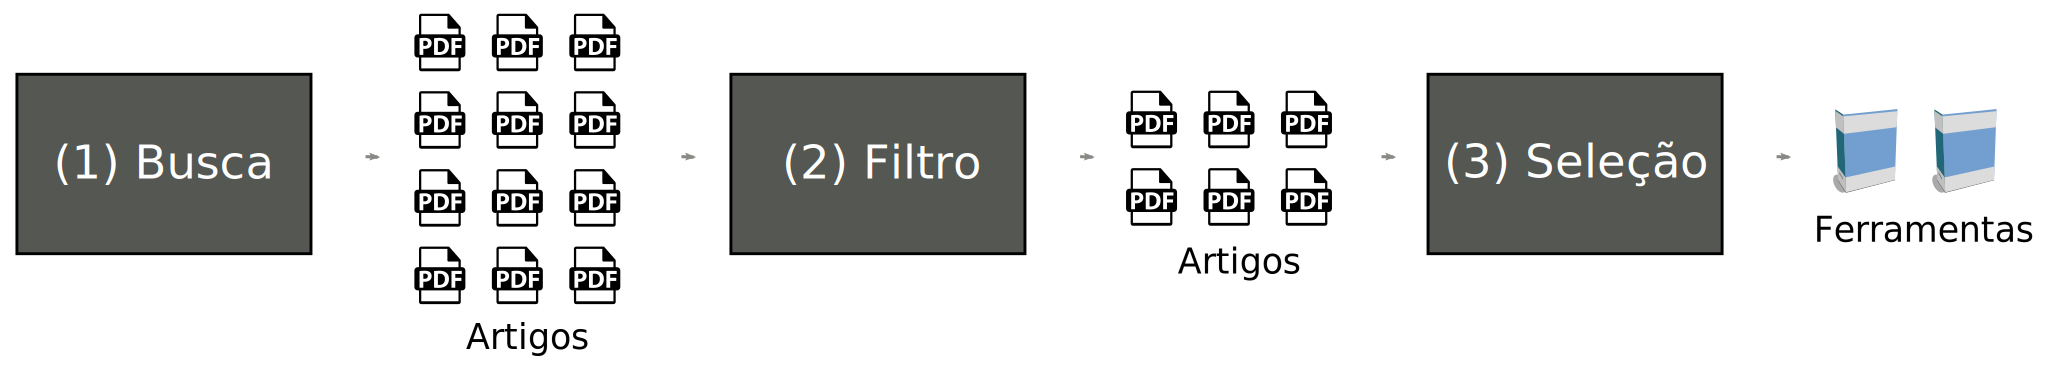
\includegraphics[scale=0.33]{imagens/revisao-estruturada.png}
  \caption{Representação gráfica da revisão estruturada}
  \label{figura-revisao-estruturada}
\end{figure}

A revisão estruturada é um processo disciplinado para seleção de artigos a
partir de critérios bem definidos, de forma que seja possível a reprodução do
estudo por parte de pesquisadores interessados.

A revisão está organizada em atividades de (1) busca de artigos (definição
das fontes de busca, definição de critérios de busca, definição de script de
busca, realização da busca nas fontes) e (2) seleção de artigos. 

No primeiro passo da revisão estruturada, as fontes de busca serão definidas,
considerando conferências que abordam o tema de interesse do estudo. 

A busca textual será realizada automaticamente, utilizando um
script\footnote{http://github.com/joenio/dissertacao-ufba-2016/blob/master/revisao-estruturada/filter}
escrito especialmente para este estudo. Esta busca seleciona os artigos que
contenham os seguintes termos:

\begin{verbatim}
  "tool" OU "framework"; E
  "download" OU "available"; E
  "http" OU "ftp"; E
  "static analysis" OU "parser".
\end{verbatim}

Uma cópia local de todos os artigos encontrados, em formato PDF, será feita.

No segundo passo, a seleção de artigos será feita com base nos artigos
encontrados pela busca no passo anterior.  Nesta seleção, pretende-se
identificar se cada artigo resulta, de fato, em publicação de ferramenta de
análise estática. Uma vez que se confirme que o artigo publica uma
ferramenta, este artigo será incluído para leitura. Ferramentas que sejam
mais abrangentes do que apenas análise estática mas que contenham esta função
em seu conjunto também serão selecionadas.

Uma vez identificados os artigos que publicaram ferramentas de análise
estática, procuramos no próprio artigo por referências de onde encontrar o
código-fonte da ferramenta. Neste contexto, algumas ações serão tomadas a
partir de algumas situações.

\begin{itemize}

  \item Se os autores afirmam que a ferramenta está disponível mas o artigo
    não contém referências de onde encontrar o código-fonte, então estes
    autores serão contactados, por email, solicitando informações de onde
    obter o código-fonte da ferramenta.

  \item Se o artigo indica onde obter o código-fonte da ferramenta, mas o acesso ao local
    indicado não está disponível, ou está disponível mas o software não se
    encontra lá, então os autores serão contactados, solicitando informações
    atualizadas de onde obter uma cópia do código-fonte da ferramenta.

  \item Artigos que indicam onde obter o código-fonte da ferramenta e a referência
    está correta. Será feito o download do código-fonte da última versão
    disponível.

\end{itemize}

Uma vez que os autores contactados por email respondam com informações sobre
local para obter o software, iremos adicionar a ferramenta ao conjunto de ferramentas
a serem analisadas.

Por fim, a ferramenta livre {\it
sloccount}\footnote{http://www.dwheeler.com/sloccount} será  utilizada para
identificar a linguagem de programação usada na implementação de cada
ferramenta selecionada.  A identificação da linguagem de programação é
necessária, pois apenas as ferramentas implementadas nas linguagens de
programação suportadas pela ferramenta Analizo serão consideradas.

\section{Coleta de dados} \label{coleta}

Serão realizadas duas etapas para identificar e mapear as ferramentas de
análise estática com código-fonte disponível: uma atividade para seleção de
ferramentas da academia, descrita na Seção \ref{ferramentas-da-academia}, e
outra atividade para seleção de ferramentas da indústria, descrita na Seção
\ref{ferramentas-da-industria}.

As ferramentas selecionadas para o estudo serão analisadas com Analizo para
extração dos valores de métricas de código-fonte.  Esta análise utilizará o
comando {\it metrics} do Analizo, que calcula métricas globais de projeto e
métricas por módulos. Este estudo levará em consideração a distribuição das
métricas por módulos.

\subsection{Ferramentas da academia} \label{ferramentas-da-academia}

A seleção de ferramentas da academia será relizada por meio de uma revisão
estruturada (seção~\ref{revisao-estruturada}). A fonte de busca para artigos
será a conferência SCAM - Source Code Analysis and Manipulation Working
Conference\footnote{http://www.ieee-scam.org} e mais uma dentre as seguintes
conferências:

\begin{itemize}
  \item ASE - Automated Software
    Engineering\footnote{http://ase-conferences.org}
  \item CSMR\footnote{A conferência CSMR tornou-se SANER - Software Analysis,
    Evolution, and Reengineering a partir da edição 2015.} - Conference on
    Software Maintenance and
    Reengineering\footnote{http://ansymore.uantwerpen.be/csmr-wcre}
  \item ICSME - International Conference on Software Maintenance and
    Evolution\footnote{http://www.icsme.org}
\end{itemize}

Todas estas conferências possuem trilhas para publicação de ferramentas e tem
como tema, áreas de estudo relacionadas à análise de programa e análise
estática, o que representa um grande potencial de encontrarmos ferramentas de
análise estática de código-fonte publicadas em suas mais de 20 edições. A
decisão de incluir apenas mais uma conferência além da conferência SCAM se
justifica pelo pouco tempo que temos para concluir este trabalho, de forma que
não seria viável incluir mais fontes.

Após download do código-fonte de cada ferramenta selecionada, em sua versão
mais recente, a ferramenta Analizo será utilizada para a coleta das métricas. 

\subsection{Ferramentas da indústria} \label{ferramentas-da-industria}

A seleção de ferramentas da indústria será feita de forma não estruturada a
partir de uma busca livre e manual no site do projeto SAMATE. As ferramentas
com código-fonte disponível, implementadas nas linguagens de programação
suportadas pelo Analizo serão selecionadas.

Após download do código-fonte de cada ferramenta selecionada, em sua versão
mais recente, a ferramenta Analizo será utilizada para a coleta das métricas. 

\section{Análise de dados} \label{analise}

Os dados coletados incluem métricas de código-fonte para cada módulo/classe de
cada ferramenta selecionada, tanto da indústria quanto da academia. As
métricas a serem analisadas e interpretadas são as métricas descritas na Seção
\ref{metricas-de-codigo}.

A linguagem R \cite{Ihaka1996}, uma linguagem de programação para cálculos
estatísticos e gráficos, será utilizada para manipulação de dados, criação de
tabelas e plotagem de gráficos. Todos os cálculos em linguagem R utilizados
neste trabalho estão disponíveis
em nosso repositório\footnote{https://github.com/joenio/dissertacao-ufba-2016/blob/master/qualificacao.R}.

\subsection{Distribuição dos valores das métricas}

Iremos calcular os percentis de cada métrica para cada ferramenta a partir dos
valores das métricas dos seus módulos, um percentil é a centésima parte dos
dados ordenados de forma crescente, iremos calcular os percentis 1, 5, 10, 25,
50, 75, 90, 95 e 99, e dentre eles iremos discutir os resultados em função dos
percentis 75, 90 e 95, assim como feito por \citeonline{Meirelles2013},
correspondendo a valores muito frequentes, frequentes e pouco frequentes,
respectivamente.

Esta discussão irá nos fornecer como resultado intervalos de referência para
métricas de código-fonte neste domínio de aplicação, estes intervalos serão
definidos a partir da interpretação manual dos percentis e serão analisados
usando modelos de regressão a fim de serem compreendidos e validados, uma
comparação com intervalos encontrados nos trabalhos relacionados (seção
\ref{trabalhos-relacionados}) também será realizada com objetivo de reforçar
estes valores.

\subsection{Cálculo de distância e modelo de aproximação} \label{distancia}

A partir da distribuição das métricas nos percentis 75, 90 e 95 e dos
intervalos de referência encontrados propomos uma abordagem para calcular o
quão distante cada ferramenta se encontra destes intervalos.  Esta abordagem
terá como base um fator de aproximação chamado {\it score} de similaridade,
este {\it score} será primeiramente calculado para os intervalos de referência
e servirão como base de comparação para o cálculo da distância de cada
ferramenta.

O {\it score} de similaridade será calculado a nível de projeto, ou seja,
teremos um único valor para cada ferramenta calculado a partir de suas várias
métricas. Para isto, iremos abstrair o significado individual de cada métrica,
o que pode não ser muito efetivo já que diferentes métricas possuem diferentes
grandezas. Para resolver este problema será feita uma normalização dos valores
das várias métricas a fim de deixá-las num mesmo intervalo, com uma certa
equivalência, seguindo uma ideia semelhante ao que é feito com a distância
euclidiana, onde todas as variáveis tem suas distâncias unificadas em um único
valor.

Os valores do {\it score} calculados a partir dos intervalos de referência
serão centralizados em 0, indicando o centro de comparação para o cálculo da
distância com cada ferramenta, desta forma, ferramentas com {\it score} acima
de 0 indicam valores piores em relação aos intervalos de referência, e
ferramentas com {\it score} abaixo de 0 indicam valores melhores do que os
intervalos de referência.

\subsection{Caracterização das ferramentas} \label{caracterizacao-das-ferramentas}

\citeonline{Novak2010} através de um estudo para construção de uma taxonomia
para ferramentas de análise estática propuseram uma classificação a partir de
uma série de categorias.

\begin{description}

  \item {\it Entrada - quais tipos de arquivos podem ser carregados na ferramenta:}
    \begin{itemize}
      \item Código-fonte - arquivos de código texto podem ser carregados
      \item Byte code - arquivos com Java Byte Code ou Microsoft
      \item Linguagem intermediária (MSIL) pode ser carregada
    \end{itemize}

  \item {\it Lançamentos ({\it Releases}) - quantos lançamentos por ano:}
    \begin{itemize}
      \item Frequentemente $>=$ 3 vezes ao ano - novas versões da ferramenta são lançadas 3 ou mais vezes por ano
      \item Ocasionalmente $<$ 3 vezes ao ano - novas versões da ferramenta são lançadas menos que 3 vezes ao ano
      \item Obsoleta 0 vezes ao ano - intervalo entre novos lançamentos é maior que 1 ano
    \end{itemize}

  \item {\it Linguagens suportadas - quais linguagens de programação a ferramenta suporta:}
    \begin{itemize}
      \item .NET - todas as linguagens compiladas em bibliotecas ou programas no framework .NET
      \item VB .NET - suporta VB.NET
      \item C\# - suporta C\#
      \item Java - suporta linguagem de programação Java
      \item C, C++ - suporta linguagem de programação C ou C++
    \end{itemize}

  \item {\it Tecnologia - quais tecnologias são usadas para procurar erros no código:}
    \begin{itemize}
      \item Dataflow - busca por erros com dataflow
      \item Sintaxe - busca por errors de sintaxe e correctness
      \item Prova de teoremas - procurar erros em provar diferentes teoremas
      \item Verificação de modelos - procurar erros com verificação de modelo
    \end{itemize}

  \item {\it Regras - conjunto de regras, quais são suportadas por diferentes código estático:}
    \begin{itemize}
      \item Estilo - inspeciona a aparência do código-fonte
      \item Naming - checa se as varáveis são nomeadas corretamente (ortografia, padroes de nomenclatura, ...)
      \item Geral - regras gerais de analise estática de código
      \item Concorrencia - erros com execução de código de concorrente
      \item Exceções - erros lançando ou não exceções
      \item Performance - erros de performance das aplicações
      \item Interoperabilidade - erros de comportamento comum
      \item Segurança - erros que podem impactar na segurança da aplicação
      \item SQL - procurar por "SQL injections" e outros erros de SQL
      \item Buffer overflow - erros de segurança, que explorar buffer overflow
      \item Manutenabilidade - regras para melhor manutenabilidade da aplicação
    \end{itemize}

  \item {\it Configurabilidade - habilidade de configurar a ferramenta:}
    \begin{itemize}
      \item Documento texto - comfiguração é feita via documento texto
      \item XML - configuração pe feita por documento XML
      \item GUI - configuraçãi é feita via interface gráfica
      \item Ruleset - ferramenta pode ligar/desligar conjunto de regras
    \end{itemize}

  \item {\it Extensibilidade - se a ferramenta pode ser extendida com regras próprias:}
    \begin{itemize}
      \item Possível - é possível extender
      \item Não possível - não é possível extender
    \end{itemize}

  \item {\it Disponibilidade - de que forma a ferramenta está disponível:}
    \begin{itemize}
      \item Código Aberto ({\it Open Source}) - a ferrament é livre e o código-fonte está disponível
      \item Grátis ({\it Free}) - a ferramenta é grátis mas o código-fonte não está disponível
      \item Comercial - a ferramenta está disponível mediante pagamento
    \end{itemize}

  \item {\it Experiência do usuário - de que forma a ferramenta pode ser usada, como é oferecida:}
    \begin{itemize}
      \item Integração com ambiente - como a ferramenta é integrada ao ambiente de trabalho
      \item Localização automática de erros no código - quando a ferramenta encontra um erro, ela leva ao local do erro
      \item Ajuda abrangente sobre falhas - se a ferramenta oferece ajuda na resolução de erros
      \item Interface de usuário - disponibilidade de uma interface de usuário
      \item Linha de comando - ela pode ser executada via linha de comando
      \item GUI - a ferramente pode ser executada em uma interface gráfica (GUI)
    \end{itemize}

  \item {\it Saída - representação dos resultados da ferramenta:}
    \begin{itemize}
      \item Arquivo texto - ferramenta pode apresentar resultados em arquivos texto
      \item Lista - ferramenta pode apresentar resultados numa interface de usuário customizada controlada em GUI
      \item Arquivo XML - ferramenta pode apresentar resultados em dados XML
      \item Arquivo HTML - ferramenta pode apresentar resultados em dados HTML
    \end{itemize}

\end{description}

Iremos utilizar algumas destas categorias na caracterização das ferramentas
selecionadas neste estudo, e vamos também caracterizar em relação à linguagem de
programação a qual foi escrita.

O Apêndice \ref{caracterizacao-ferramentas} traz uma caracterização inicial
das ferramentas segundo às categorias acima.

\section{Cronograma} \label{cronograma}

\begin{table}[h!]
  \centering
  \begin{tabular}{| l | c | c | c | c | c |}
    \hline
    {\bf Atividade}                                & Jul     & Ago       & Set      & Out      & Nov      \\
    \hline
    \hline
    Qualificação                                   &\checkmark&          &          &          &          \\
    \hline
    Análise da distribuição das métricas           &\checkmark&          &          &          &          \\
    \hline
    Definição dos valores de referência            &          &\checkmark&          &          &          \\
    \hline
    Cálculo de distância e modelo de aproximação   &          &\checkmark&          &          &          \\
    \hline
    Revisão estruturada com mais uma conferência   &          &\checkmark&          &          &          \\
    \hline
    Adicionar coleta/análise com novas ferramentas &          &          &\checkmark&          &          \\
    \hline                                                                                     
    Caracterização das ferramentas                 &          &          &\checkmark&          &          \\
    \hline                                                                                     
    Caracterização da complexidade estrutural      &          &          &          &\checkmark&          \\
    \hline                                                                                     
    Evolução da ferramenta Analizo                 &\checkmark&\checkmark&\checkmark&\checkmark&\checkmark\\
    \hline
    Defesa                                         &          &          &          &          &\checkmark\\
    \hline
  \end{tabular}
\end{table}


%------------------------------------------%

\xchapter{Analizo}
{Este capítulo apresenta o software de análise estática Analizo utilizado
neste estudo para coleta de dados.}
\label{analizo}

Analizo \cite{terceiro2010analizo} é um conjunto de ferramentas para análise de código-fonte e
visualização com suporte a múltiplas linguagens de programação, software livre,
extensível e capaz de lidar com código-fonte não mais compilável. A capacidade
de lidar com código-fonte não mais compilável permite analisar código-fonte
com erros de sintaxe, com referências a bibliotecas não mais disponíveis, ou
que usem bibliotecas com mudanças de API.

%Ela será a ferramenta utilizada por nós durante este estudo para análise do
%código-fonte das ferramentas selecionadas, a decisão pela ferramenta Analizo
%se deu por conta dela ser também a escolha utilizada nos trabalhos
%relacionados (seção \ref{trabalhos-relacionados}) onde estamos nos apoiando,
%além disso, Analizo também tem sido utilizada em diversos estudos
%desenvolvidos em nosso grupo de pesquisa (seção \ref{trabalhos-analizo}).

%% \section{Arquitetura do Analizo}
%% 
%% A arquitetura do Analizo é apresentada na Figura \ref{arquitetura-analizo}
%% através de uma representação {\it Layered Style} \cite{Clements2002}, cada
%% camada no diagrama usa apenas os serviços oferecidos pela camada diretamente
%% abaixo dela.
%% 
%% \begin{figure}[h]
%% \center
%% 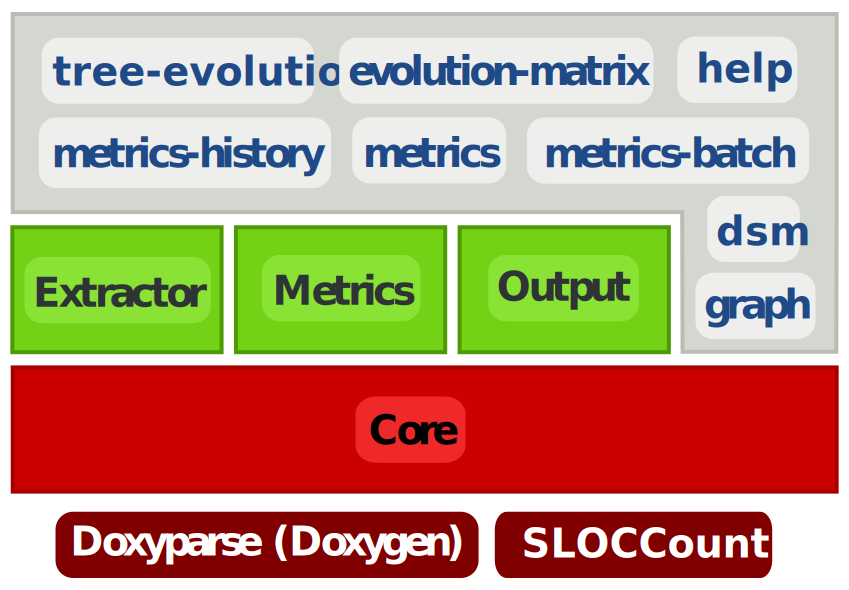
\includegraphics[scale=0.3]{imagens/analizo-architecture.png}
%% \caption{Arquitetura do Analizo, usando Layered Style \cite{Clements2002}}
%% \label{arquitetura-analizo}
%% \end{figure}
%% 
%% O {\it Core} contém as estruturas de dados usadas para armazenar informações a
%% respeito do código-fonte sendo analisado, lista de módulos\footnote{o
%% conceito ``módulo'' é usado como um termo abrangente para designar diferentes
%% tipos de estruturas usados em desenvolvimento de software, como classes e
%% arquivos fonte C}, elementos dentro de cada módulo (atributos, variáveis,
%% métodos, funções) e informações de dependência (chamada, herança, etc). Esta
%% camada implementa a maior parte da lógica de negócio do Analizo, e não depende
%% de nenhuma outra camada.
%% 
%% A camada {\it Extractor} lida com as informaçoes de código-fonte obtidas pelas
%% diferentes estratégias implementadas no Analizo. Os extratores obtém
%% informações do código-fonte e armazenam em estruturas de dados na camada {\it
%% Core}. Adicionar um novo extrator requer apenas a criação de uma nova subclasse
%% que faça interface com uma ferramenta externa ou que ela própria realize análise
%% de código-fonte.
%% 
%% Atualmente existem dois extratores, ambos fazem interface
%% com ferramentas externas de análise estática de código-fonte:
%% 
%% \begin{itemize}
%% 
%%   \item {\it Analizo::Extractor::Doxyparse} é uma interface para o Doxyparse,
%%   um parser de código-fonte para C, C++ e Java desenvolvida por nosso grupo de
%%   pesquisa\cite{Costa2009}. Doxyparse é baseado no
%%   Doxygen\footnote{doxygen.org}, um sistema de documentação multi-linguagem.
%% 
%%   \item {\it Analizo::Extractor::Sloccount} é uma interface para o
%%   Sloccount\footnote{dwheeler.com/sloccount} desenvolvido por David A. Wheeler,
%%   uma ferramenta que calcula o número efetivo de linhas de código.
%% 
%% \end{itemize}
%% 
%% A camada {\it Metrics} processa as estruturas de dados do {\it Core} para
%% calcular métricas, até o momento Analizo suporta um conjunto razoável de
%% métricas (listadas na Seção \ref{metricas}), uma representação desta camada
%% pode ser vista no diagrama da Figura \ref{arquitetura-metrics-analizo}.
%% 
%% A camada {\it Output} é responsável por lidar com diferentes formatos de
%% arquivos.  Atualmente, apenas o formato DOT é implementado no Analizo para
%% representar grafo de dependencia, adicionar novos formatos é simplesmente
%% adicionar novas classes nesta camada.
%% 
%% \begin{figure}[h]
%% \center
%% 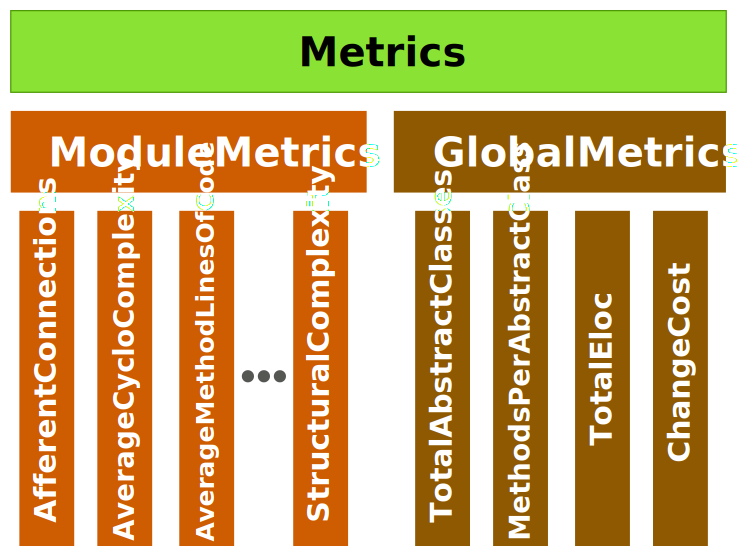
\includegraphics[scale=0.4]{imagens/analizo-metrics-architecture.png}
%% \caption{Arquitetura do módulo metrics em detalhes, usando Layered Style \cite{Clements2002}}
%% \label{arquitetura-metrics-analizo}
%% \end{figure}
%% 
%% A última camada, {\it Tools}, fornece um conjunto de ferramentas de linha de comando que
%% constituem a interface do analizo, tanto para usuários finais quanto para
%% aplicações de mais alto nível. Estas ferramentas usam serviços providos pelas
%% outras camadas: eles instanciam as estruturas de dados do {\it Core},
%% inicializam um ou mais extratores, opcionalmente executam o processador de
%% métricas, instanciam um módulo de formato de saída, e gerencia todos eles para
%% prover o resultado desejado. A maioria das funcionalidades descritas na Seção
%% \ref{funcionalidades} são implementadas nesta camada.
%% 
%% Estas ferramentas são pensadas na filosofia UNIX: fazem uma tarefa
%% especializada e geram uma saída que pode ser utilizada como entrada para outras
%% ferramentas, seja para o próprio Analizo ou para ferramentas externas. Algumas
%% das ferramentas implementadas no Analizo são feitas consumindo saída gerada por
%% outra ferramenta, outras são desenhadas para prover saída em formato específico
%% para aplicações externas, por exemplo, programas para desenho de grafos ou
%% visualização de dados.

\section{Funcionalidades}\label{funcionalidades}

\begin{itemize}

\item {\bf Análise de código-fonte multi-linguagem}

Atualmente Analizo suporta análise de código-fonte escrito em C, C++ e Java.
Entretanto, pode ser facilmente estendido para suportar outras linguagens pois
pode potencialmente suportar as inúmeras outras linguagens suportadas pelo Doxygen.

\item {\bf Métricas}\label{metricas}

O Analizo suporta tanto métricas em nível de projeto, que é calculada para todo o projeto,
quanto métricas em nível de módulos, que é calculado individualmente para cada módulo.
No nível de projeto, Analizo também provê estatística descritiva básica para cada métrica em
nível de módulo: soma, média, mediana, moda, desvio padrão, variância, skewness e kurtosis da
distribuição, valores mínimo e maximo. As seguintes métricas são suportadas até o momento:

\begin{itemize}

  \item Métricas em nível de projeto: Change Cost, Total Abstract Classes,
  Total Coupling Factor, Total Effective Lines of Code, Total Lines of Code,
  Methods per Abstract Class, Total Number of Modules, Total number of modules
  with at least one defined attributes, Total number of modules with at least
  one defined method, Total Number of Methods.

  \item Métricas em nível de módulo: Afferent Connections per Class, Average
  Cyclomatic Complexity per Method, Average Method Lines of Code, Argument with
  'nonnull' attribute passed null, Average Number of Parameters per Method,
  Allocator sizeof operand mismatch, Assigned value is garbage or undefined,
  Bad deallocator, Bad free, Coupling Between Objects, Dead assignment,
  Divisions by zero, Double free, Depth of Inheritance Tree, Dereference of
  null pointer, Dereference of undefined pointer value, Potential buffer
  overflow in call to 'gets', Lack of Cohesion of Methods, Lines of Code,
  Memory leak, Max Method LOC, Number of Attributes, Number of Children, Number
  of Methods, Number of Public Attributes, Number of Public Methods,
  Out-of-bound array access, Offset free, Potential insecure temporary file in
  call 'mktemp', Response for a Class, Result of operation is garbage or
  undefined, Return of stack variable address, Stack address stored into global
  variable, Structural Complexity, Undefined allocation of 0 bytes,
  Use-after-free, Uninitialized argument value.

\end{itemize}

É possível especificar que certos diretórios dentro do projeto não devem ser
analisados, de forma que o Analizo ignore tais arquivos durante a análise e o
cálculo de métricas.

%\item {\bf Processamento em lote}\label{lote}
%
%A maioria dos estudos quantitativos em engenharia de software envolve aquisição
%de métricas de código-fonte de um grande número de projetos, processar cada
%projeto individualmente é pouco prático, passível de erros e difícil de
%repetir. Analizo pode processar multiplos projetos em lote e produzir arquivo
%de dados CSV com métricas de cada projeto, bem como um resumo com as métricas
%em nível de projeto de todos os projetos. Estes arquivos de dados podem ser
%facilmente importados em ferramentas de estatística ou planilhas para análise
%futura. Esta capacidade de processar em lote pode também ser utilizada para
%analisar várias versões de um mesmo projeto, especialmente útil em estudos
%sobre evolução de software.

%% Este processamento em lote pode se beneficiar de processamento paralelo dando
%% mais agilidade e na análise e reduzindo o tempo total de processamento.  A
%% saída pode ser também escrita diretamente em um banco de dados relacional ao
%% invés de gerar arquivos CSV. Outro recurso voltado à performance é um sistema
%% de cache para as informações previamente calculadas, evitando repetição de
%% processamento.

%\item {\bf Histórico de métricas}
%
%Algumas vezes pesquisadores precisam processar o histórico de projetos de
%software de uma forma mais escalável. Analizo pode processar repositórios de
%controle de versão e prover arquivo de dados CSV com valores de métricas para
%cada revisão onde o código-fonte foi alterado no projeto, ou pode também gravar
%os valores diretamente num banco de dados ao invés de usar arquivos CSV. Repositórios Git e
%Subversion são suportados diretamente, repositórios CVS devem ser convertidos
%para Git de forma manual.

%\item {\bf Grafo de dependência}
%
%Analizo pode gerar saída com informações sobre dependência entre as entidades
%do projeto em um formato adequado para processamento por ferramentas de
%renderização de grafos do Graphviz\footnote{graphviz.org}. A Figura
%\ref{sample-graph} apresenta um exemplo de grafo desenhado pela ferramenta {\it
%dot} do Graphviz a partir da saída gerada pelo Analizo {\it graph}.
%
%\begin{figure}[h]
%\center
%\includegraphics[scale=0.4]{imagens/sample-graph.png}
%\caption{Exemplo de grafo de dependência}
%\label{sample-graph}
%\end{figure}

%% \item {\bf Matriz de evolução}
%% 
%% Outra funcionalidade útil do Analizo é a visualização de matrizes de evolução
%% \cite{Lanza2001}. Ao processar cada release de um projeto (ver Seção
%% \ref{lote}), o usuário pode solicitar a criação de uma matriz de evolução a
%% partir de arquivos de dados individuais. A Figura \ref{sample-evolution-matrix}
%% apresenta um exemplo de uma matriz produzida pelo Analizo.
%% 
%% \begin{figure}[h]
%% \center
%% \includegraphics[scale=0.2]{imagens/sample-evolution-matrix.png}
%% \caption{Exemplo de matriz de evolução}
%% \label{sample-evolution-matrix}
%% \end{figure}
%% 
%% \item {\bf Matriz de estrutura de projeto}
%% 
%% Uma funcionalidade recente do Analizo é a representação visual do
%% relacionamento entre os módulos do projeto em forma de uma matriz de estrutura
%% de projeto ({\it Design Structure Matrix}) \cite{Maccormack2006}, uma DSM é a
%% representação de um grafo de dependência em forma de uma matriz quadrada. Um
%% exemplo gerado pelo Analizo pode ser visto na Figura \ref{sample-dsm}.
%% 
%% \begin{figure}[h]
%% \center
%% \includegraphics[scale=0.3]{imagens/sample-dsm.png}
%% \caption{Exemplo de matriz de estrutura de projeto}
%% \label{sample-dsm}
%% \end{figure}

\end{itemize}

\section{Uso em trabalhos de pesquisa}
\label{trabalhos-analizo}

Analizo tem sido extensivamente usado por nosso grupo de pesquisa em diversos
estudos:

\begin{itemize}

  \item \cite{amaral2009analise} usou o grafo de dependencia gerado pelo Analizo para
  gerar uma matriz de evolução em um estudo de caso com o projeto VLC.

  \item \cite{costa2009extracao} fez uma comparação entre diferentes estratégias para
  extração de informação de dependencias entre módulos do código-fonte,
  resultando no desenvolvimento do Doxyparse - o extrator baseado no Doxygen do
  Analizo.

  \item \cite{terceiro2009structural} usou métricas em um estudo exploratório sobre a
  evolução da complexidade estrutural em projetos de software livre escritos em
  C.

  \item \cite{morais2009kalibro} usou a ferramenta de métricas do Analizo como backend
  para o Kalibro, um software para avaliação e observação de métricas de código-fonte.
  
  \item \cite{terceiro2010empirical} usou o processamento de histórico de métricas para
  realizar um estudo exploratório sobre a evolução da complexidade estrutural em
  7 projetos de servidor web de diferentes tamanhos.

  \item \cite{meirelles2010astudy} usou o processamento em lote do Analizo para
  processas o código-fonte de mais de 6000 projetos de software livre do
  repositório Sourceforge.net.

  \item \cite{meirelles2011semiautomatic} usou o Analizo em um estudo sobre impacto de
  métricas de código-fonte na atratividade de projetos de softwares livres.

  \item \cite{terceiro2012understanding} usou o Analizo para investigar fatores
  que influenciam na evolução da complexidade estrutural em projetos de software
  livres.

  \item \cite{silva2012concernbased} usou o Analizo para minerar 16000 revisões de
  repositórios de projetos de software para investigar o potencial de uma nova
  métrica chamada Lack of Concern-based Cohesion.

  \item \cite{ronaldo2015estudo} utilizou o Analizo para extrair métricas de
  código-fonte de 14 versões do sistema Android e estudar a evoluçao da API e
  seus aplicativos.

\end{itemize}

A maioria destes trabalhos contribuíram com melhorias para o Analizo, fazendo
dele uma ferramenta bastante apropriada para pesquisas envolvendo análise de código-fonte,
sendo útil tanto para pesquisadores trabalhando com análise de código-fonte
quanto para profissionais que precisam analisar seus projetos em busca de
potenciais problemas ou melhorias.

Analizo é software livre, distribuído sob a licença GNU General Public License
versão 3. Seu código-fonte, bem como pacotes binários, manuais e tutoriais
podem ser obtidos em \url{http://www.analizo.org}. Todas as ferramentas são
auto-documentadas e podem ser consultadas como páginas de manual UNIX. Analizo
é escrito em Perl, sua última versão 1.19.1 lançada em 01 de Setembro de 2016
foi a versão utilizada neste estudo.

%% \subsection{Analizo}
%% 
%% Numa primeira análise dos valores coletados pelo Analizo notamos uma anomalia
%% nos valores da métrica CBO, o que nos levou a investigar de perto os motivos,
%% esta anomalia se apresentava como valores extremamente altos para esta métrica,
%% bastante discrepante com as demais métricas calculadas.
%% 
%% Para entender se estes valores estavam corretor ou não, utilizamos uma outra
%% ferramenta para cálculo das métricas, em nossos estudos encontramos e
%% utilizamos uma versão de avaliação da ferramenta {\it SciTools
%% Understand}\footnote{http://scitools.com/trial-download-3} em sua versão
%% ``4.0.853'' em Linux 64 bits. Os dados extraídos por esta ferramenta podem ser
%% encontrados em nosso
%% repositório\footnote{http://github.com/joenio/dissertacao-ufba-2016/tree/master/dataset/Understand
%% SciTools}. Eles demonstraram que os valores calculados pelo Analizo estavam
%% bastante alto em comparação com as demais métricas.
%% 
%% Assim, descobrimos que o Analizo tinha de fato um erro no cálculo da métrica
%% CBO, erro que foi corrigido durante este estudo e disponibilizado na versão
%% mais recente do Analizo, versão que está sendo utilizada aqui.


%------------------------------------------%

\xchapter{Disponibilidade dos projetos de software acadêmico de análise estática}
{Este capítulo apresenta um estudo sobre disponibilidade de acesso (download)
dos projetos de software de análise estática publicados nas conferências de
Engenharia de Software ASE e SCAM até o ano de 2015.}
\label{estudo1}

Este estudo selecionou, através de uma revisão de literatura em conferências da
Engenharia de Software, 60 projetos de software de análise estática
desenvolvidos e publicados nas conferências ASE e SCAM, caracterizou estes
projetos em relação a disponibilidade para download, bem como a capacidade de
acesso ao código fonte e a forma como são distribuídos e licenciados.

A seção \ref{estudo1:introducao} contextualiza o estudo,
a seção \ref{estudo1:fundamentacao} apresenta os conceitos teóricos necessários para compreensão do trabalho,
a seção \ref{estudo1:definicao} descreve o objetivo e apresenta as questões de pesquisa,
a seção \ref{estudo1:planejamento} apresenta um planejamento do estudo,
as seções \ref{estudo1:preparacao} e \ref{estudo1:coleta} apresentam detalhes sobre a preparação e execução da coleta de dados,
as seções \ref{estudo1:analise} e \ref{estudo1:interpretacao} apresentam a análise e interpretação dos dados e
a seção \ref{estudo1:conclusoes} traça as conclusões finais deste estudo.

\section{Introdução e Motivação} \label{estudo1:introducao} % {{{

Os projetos de software desenvolvidos na academia sofrem de {\it
``dysfunctional chaotic churn''} \cite{howison2015understanding}.

Na prática, isso significa que há muitos projetos com características e
funcionalidades parecidas, com poucos usuários, com ciclos de vida curtos, e
encerrados quando o financiamento inicial termina, bem como, comunidades
desconectadas e paralelas, incompatibilidades entre projetos em um mesmo
domínio, e tentativas aparentemente não coordenadas de ``reiniciar'' tudo ({\it
re-boots}).

Parte deste problema tem sido atribuido a falta de treinamento em boas práticas
de desenvolvimento de software por parte dos cientistas e pesquisadores
\cite{wilson2017good}. Algo que, a princípio, não afeta os cientistas da
Engenharia de Software, visto que estes possuem formação e acesso a práticas de
desenvolvimento e estão inseridos num contexto voltado para a compreensão e
melhoria dos processos de desenvolvimento de software, tanto do ponto de vista
teórico, quanto prático.

Sabendo disso, e atentando para o fato que a grande parte do desenvolvimento de
software acadêmico é realizado pelos próprios cientistas \cite{hettrick2014uk,
momcheva2015software}, surge a preocupação de avaliar o quanto os projetos de
software desenvolvidos nas pesquisas de Engenharia de Software sofrem desse
problema, percebido por \citeonline{howison2015understanding} como
``dysfunctional chaotic churn''.

% }}}

\section{Fundamentação} \label{estudo1:fundamentacao} % {{{

\subsection{Software acadêmico}

São projetos de software desenvolvidos durante pesquisas científicas publicados
na literatura acadêmica, normalmente utilizados para coleta ou análise de
dados, podendo ser feito com objetivo de ser utilizado por outros
pesquisadores, e em algumas ocasiões sendo o software uma contribuição primária
para a Ciência \cite{howison2011scientific}.

\subsection{Disponibilidade}

Disponibilidade neste estudo está relacionada a URL do projeto de software,
indicando se o software está disponível na URL indicada pelos seus autores e de
que forma os projetos estão disponíveis, binários ou código fonte, quais
licenças são utilizadas, entre outras questões relacionadas à distribuição.

% }}}

\section{Definição} \label{estudo1:definicao} % {{{

Sabemos quantos projetos de software acadêmico de análise estática publicados
nas conferências de Engenharia de Software ASE e SCAM permanecem disponíveis
hoje? E como estão disponíveis?

\subsection{Definição do Objetivo}

\begin{description}
  \item{\bf Objeto de estudo.}
     O objeto de estudo são projetos de software acadêmico de análise estática.
  \item{\bf Propósito.}
    O propósito é caracterizar.
  \item{\bf Perspectiva.}
    A perspectiva considerada é a do cientista usuário final.
  \item{\bf Foco de qualidade.}
    O principal aspecto de qualidade estudado é a disponibilidade dos projetos.
  \item{\bf Contexto.}
    O estudo foi conduzido com publicações das conferências de Engenharia de Software ASE e SCAM.
\end{description}

\subsection{Sumário da Definição}

Analisar os \textit{projetos de software acadêmico de análise estática}
com o propósito de \textit{caracterizar}
com respeito a \textit{disponibilidade}
na perspectiva de \textit{cientistas usuários finais}
no contexto de \textit{conferências de Engenharia de Software ASE e SCAM}.

\subsection{Questões de Pesquisa}

Neste estudo as seguintes questões de pesquisa, a respeito dos projetos de
software acadêmico de análise estática publicados nas conferências ASE e SCAM,
serão investigadas:

\newcommand{\EstudoUmQuestaoUm}{
  Os projetos de software acadêmico de análise estática publicados nas conferências ASE e SCAM possuem alguma presença oficial online?
  %requisito para avaliar qualidade interna dos projetos
}
\newcommand{\EstudoUmQuestaoDois}{
  Os projetos de software academico de análise estática publicados nas conferências ASE e SCAM estão disponíveis para download?
  %requisito para uso
}
\newcommand{\EstudoUmQuestaoTres}{
  É possível ter acesso ao código fonte dos projetos de software de análise estática publicados nas conferências ASE e SCAM?
  %requisito para avaliar qualidade interna dos projetos
}
\newcommand{\EstudoUmQuestaoQuatro}{
  Os projetos de software com código fonte disponível podem ser adaptados para atender necessidades emergentes?
  %requisito para usar em novas pesquisas
}

\begin{description}
  \item [Q1:] \EstudoUmQuestaoUm
  \item [Q2:] \EstudoUmQuestaoDois
  \item [Q3:] \EstudoUmQuestaoTres
<<<<<<< HEAD
=======
  \item [Q4:] \EstudoUmQuestaoQuatro
>>>>>>> 438785c3cf436efa2037aff01be707be180abd75
\end{description}

\subsection{Métricas}

Para responder às questões de pesquisas, as seguintes métricas serão usadas:

\begin{enumerate}
  \item Número de projetos com identificação de nome e URL
  \item Número de projetos com URL disponível
  \item Número de projetos disponível para download
  \item Número de projetos com código fonte disponível
  \item Número de projetos com permissão explícita de contribuição via código fonte
\end{enumerate}

% }}}

\section{Planejamento do Estudo} \label{estudo1:planejamento} % {{{

Este estudo foi realizado em duas etapas principais, conforme ilustrado na
Figura \ref{estudo1-etapas}, a primeira etapa com o objetivo de selecionar
artigos com publicação de software acadêmico de análise estática e a segunda
etapa com o objetivo de caracterizar estes projetos de software, especialmente
em relação a disponibilidade de acesso.

\begin{figure}[h]
  \center
  
\includegraphics[scale=0.4]{imagens/estudo1-etapas.png}
  \caption{Etapas do estudo e seus resultados}
  \label{estudo1-etapas}
\end{figure}

As seções à seguir apresentam o planejamento dessas duas etapas.

\subsection{Revisão de literatura com publicação de software de análise estática}

Nesta primeira etapa realizamos uma revisão de literatura com o objetivo de
encontrar artigos mencionando software de análise estática entre os resultados
do estudo. A revisão foi organizada em três passos, detalhados à seguir.

%-- busca, filtro e seleção -- cada etapa 
%um conjunto de artigos que atendem aos critérios de inclusão e
%exclusão definidos naquela atividade, estes artigos são utilizados como entrada
%na etapa seguinte.  A última atividade -- seleção -- gera como saída o conjunto
%final de artigos com publicação de software acadêmico de análise estática.

\subsubsection{Passo 1: Escopo}

%de Engenharia de Software utilizadas como ponto de partida na revisão de literatura,

Neste momento definimos quais serão as conferências utilizadas como fonte dos
artigos da revisão de literatura, todas as publicações serão selecionadas e
incluídas no conjunto inicial de artigos da revisão, iniciando pela primeira
edição de cada conferência indo até a última edição, mas tendo como limite uma
data previamente definida.

Esta data deve indicar o ano limite a ser considerado na seleção e inclusão de
publicações ao conjunto inicial de artigos da revisão de literatura, serão
consideradas todas as publicações de cada conferência até o ano limite,
incluindo os artigos publicados neste ano.

As conferências devem ser selecionadas tendo em vista aumentar e potencializar
o número total de projetos de software acadêmico do domínio de aplicação de
interesse do estudo, neste caso, análise estátic. Deve-se buscar
preferencialmente conferências com bom histórico de publicações sobre o domínio
de aplicação do estudo.

É importante investigar o histórico de cada conferência com atenção ao nome do
evento em cada edição, não é raro que conferências com muitos anos de
existência mudem de nome ao longo do tempo, nestes casos deve-se adotar o nome
da conferência mais recente e consider todas as edições anteriores com este
mesmo nome.

%, ou
%seja, o nome mais recente, mesmo que isto inclua conferencias distintas, é
%adotado para todas as edições.

Uma vez definidos a data limite e as conferências deve-se fazer o download de
todos os artigos até a data limite, os arquivos devem ser organizados em pastas
por nome e ano da conferência. Os títulos de todos os artigo, a correspondente
conferência e o ano de publicação devem ser registrados e armazenados em
arquivos ou banco de dados, neste estudo fizemos uso do
LibreOffice Calc\footnote{\url{https://www.libreoffice.org}}.

%O formato desta planilha , sobre a estrutura de pastas utilizadas
%para armazenar os artigos, e onde encontrar o arquivo utilizado neste estudo
%para a coleta destes dados pode ser consultado em detalhes no Apêndice
%\ref{reproducibilidade-do-estudo}.

\subsubsection{Passo 2: Triagem Automática} \label{estudo1:planejamento:filtro}

O escopo definido no passo anterior irá, potencialmente, resultar num enorme
conjunto de artigos para revisão, assim, o objetivo da triagem é reduzir este
número mantendo apenas as publicações relevantes para os objetivos do estudo.

Isto é feito através de uma busca textual no conteúdo de cada artigo, esta
busca deve ser realizada de forma automática com auxilio de ferramentas de
software para busca textual em conteúdo de arquivos pdf. Ela irá pesquisar um
conjunto de palavras chave representando os critérios de inclusão da triagem,
apenas os artigos combinando com estes critérios serão incluídos, conforme
Tabela \ref{criterios-triagem}.

\begin{table}[h]
\caption{Critérios de inclusão e palavras chave para a triagem dos artigos.}
\centering
\begin{tabular}{ l l }
  \hline
  Critério                                 & Palavras chave                        \\
  \hline
  Menciona projeto, software ou ferramenta & {\tt tool} ou {\tt framework}         \\
  Disponibiliza download do projeto        & {\tt download} ou {\tt available}     \\
  Identifica URL do projeto                & {\tt http} ou {\tt ftp}               \\
  Domínio de análise estática              & {\tt static analysis} ou {\tt parser} \\
  \hline
\end{tabular}
\label{criterios-triagem}
\end{table}

Se um determinado artigo não combinar com algum dos critérios ele será
excluído, assim, ao final deste passo o número total de artigos será reduzido
em um conjunto menor contendo apenas as publicações relevantes para o objetivo
do estudo

%contendo apenas artigos com ocorrencia das palavras chave
%relacionadas a cada um dos critérios, este conjunto reduzido é passado para a
%etapa seguinte.

\subsubsection{Passo 3: Extração}

Os artigos serão inspecionados manualmente em busca de software acadêmico de
análise estática entre os resultados do estudo, os critérios de inclusão tem
como objetivo incluir apenas os projetos de software identificados minimamente
pelos seus autores com nome e URL para download, conforme Tabela
\ref{criterios-extracao}.

\begin{table}[h]
\caption{Critérios de inclusão para o passo de extração dos artigos (adaptado de \citeonline{howison2016software}).}
\centering
\begin{tabular}{ l p{12cm} }
  \hline
  Critério         & Explicação \\
  \hline
  Identificável    & É possível identificar um projeto de software entre as contribuições do artigo? (ex: ``um programa que nós escrevemos``, ``nossa implementação``, ``nosso protótipo'') \\
  Disponível       & Podemos encontrar menção a URL do projeto de software para download? \\
  \hline
\end{tabular}
\label{criterios-extracao}
\end{table}

Os nomes e endereços URL de cada projeto encontrado durante a inspeção manual
devem ser extraídos e armazenados junto aos dados já coletados nos passos
anteriores da revisão. A inspeção deve incluir a leitura do título, introdução,
resultados e conclusões de cada artigo, caso necessário utiliza-se as outras
seções do artigo. Alguns artigos descrevem a contribuição de software acadêmico
em seções específicas, é comum, por exemplo, encontrar artigos fazendo uso de
notas de rodapé para indicar a URL do software.

Os artigos devem ser inspecionados num ciclo, um por vez, até chegar ao útlimo
artigo dentre os selecionados no passo anterior, ao final da extração teremos
dados de um conjunto de projetos de software acadêmico de análise estática,
incluindo nome do projeto e URL para download. Estes dados extraídos devem ser
atualizados nos arquivos ou banco de dados já utilizados nos passos anteriores.

%A planilha LibreOffice Calc utilizada como apoio
%na revisão foi atualizada com o nome do software publicado no artigo
%correspondente.
%de artigos com publicação de

%Os critérios de seleção da Tabela \ref{criterios-selecao} foram adaptados do
%trabalho de \citeonline{howison2016software}, que fez uma revisão de literatura
%da Biologia em busca de menções a software acadêmico para evidenciar problemas
%de visibilidade e de uso.

\subsection{Caracterização dos projetos de software acadêmico de análise estática}

Os dados coletados na revisão de literatura, devidamente armazenados em
arquivos ou banco de dados, inclui projetos de software acadêmico de análise
estática, identificados com nome e URL, nome e ano da conferência e
título do artigo onde foi publicado.

Estes dados deverão ser extraídos para uma nova estrutura de armazenamento
projetada para receber informações adicionais dos projetos, conforme Tabela
\ref{esquema-caracteristicas}, essas informações serão coletadas em documentos
relacionados aos projetos, como website, manuais, repositórios e código fonte.

\begin{table}[h]
\caption{Esquema para caracterização dos projetos de software acadêmico}
\centering
\begin{tabular}{ l p{11cm} }
  \hline
  Característica           & Explicação \\
  \hline
  Nome do software         & O nome do projeto de software \\
  URL                      & Endereço web do software ou projeto, site ou repositório de código fonte, com o software disponível \\
  Título do artigo         & Título do artigo onde o software é citado como contribuição, seja principal ou secundária \\
  Nome do evento           & Nome da conferência onde o software foi publicado \\
  Ano do evento            & Ano da edição da conferência onde o artigo foi publicado \\
  Descrição do software    & A descrição do projeto de software \\
  Acesso                   & Podemos acessar a URL do projeto agora? Pode receber os seguintes valores: Sem Acesso, Acesso Pago, Acesso Gratuito \\
  Distribuição             & Como o software é distribuído e pode ser acessado? Pode receber os seguintes valores: gratis, livre, proprietário \\
  Código fonte disponível  & É possível acessar o código fonte de alguma forma? \\
  Licença                  & O software deixa explícito qual licença é distribuído? \\
  Código fonte             & Em qual linguagem de programação o software acadêmico foi desenvolvido \\
%  Entradas suportadas      & Qual o tipo de entrada suportada pelo software de análise estática \\
%  Linguagens suportadas    & Quais linguagens de programação o software de análise estática suporta como entrada \\
  \hline
\end{tabular}
\label{esquema-caracteristicas}
\end{table}

O primeiro documento consultado deve ser o website indicado pela URL, esta
consulta resultará em novos documentos, como, manuais de uso, informações sobre
desenvolvimento, código fonte, notas de lançamento, entre outros. Cada um
destes documentos devem ser inspecionados em busca de informações para
caracterização dos projetos segundo a Tabela \ref{esquema-caracteristicas}.

%e documentos para download no
%site, estes documentos, quando disponíveis, também foram consultados, estes
%documentos estão normalmente disponíveis em formato txt, pdf ou doc.
%Quando disponível, o código fonte também foi inspecionado em busca de
%informações, alguns projetos distribuem junto ao código fonte documentos e
%manuais, outros documentam informações sobre o projeto no próprio código.

A coleta sobre a linguagem de programação em que projeto está escrito deve ser
realizada de maneira automática através de alguma ferramenta de análise de
código fonte, como por exemplo o software livre
\texttt{sloccount}\footnote{http://www.dwheeler.com/sloccount}.

% }}}

\section{Preparação} \label{estudo1:preparacao} % {{{

Nesta seção apresentamos a preparação do estudo para a realização da coleta de
dados.

\subsection{Revisão de literatura com publicação de software de análise estática}

\subsubsection{Passo 1: Escopo}

Seguindo o planejamento descrito em \ref{estudo1:planejamento}, definimos como
fonte de busca as conferências SCAM\footnote{\url{http://www.ieee-scam.org}}
({\it Source Code Analysis and Manipulation Working Conference}) e
ASE\footnote{\url{http://ase-conferences.org}} ({\it Automated Software
Engineering}), ambas conferências com um grande histórico de edições, definimos
como data limite o ano de 2015.

Buscamos descobrir onde os artigos estão disponíveis para download, as
publicações da conferência SCAM estão todas disponibilizadas no IEEE, a
conferência ASE possui algumas edições no IEEE outras na ACM, os endereços URL
de cada edição de cada conferência estão documentadas no Apêndice
\ref{reproducibilidade-do-estudo}.

Até o ano de 1996 a conferencia ASE chamava-se KBSE - Knowledge-Based Software
Engineering Conference e a partir de 1997 passou a chamar-se ASE - Automated
Software Conference, teve sua primeira edição no ano de 1991 e o SCAM apenas em
2001.

\subsubsection{Passo 2: Triagem Automática}

%Definimos as palavras chave para a execução do filtro conforme planejado com
%o fim de selecionar apenas os artigos que casam com os critérios definidos
%na , estes critérios e as palavras chave
%associado à cada um são apresentados na Tabela \ref{criterios-filtro}.

%Estas palavras foram escolhidas de forma empírica e contam com experiência
%prévia na área de análise estática, notamos que usualmente os autores de
%software acadêmico de análise estática mencionam contribuição em software
%fazendo menção utilizando estes termos, de forma que consideramos que a
%aplicação deste filtro em outros domínios necessita de adaptações.

Implementamos o script para execução da triagem automática a partir dos
critérios definidos no planejamento, Seção \ref{estudo1:planejamento:filtro},
este script utiliza como base o software livre
\texttt{pdftotext}\footnote{\url{https://en.wikipedia.org/wiki/Pdftotext}} para
converter o conteúdo pdf dos arquivos em texto antes de realizar o filtro pelas
palavras chave.

\subsubsection{Passo 3: Extração}

Criamos uma planilha LibreOffice Calc para coletar os dados de cada passo da
revisão de literatura com as seguintes colunas:

\begin{description}
  \item[Evento] Nome e ano da conferência de Engenharia de Software.
  \item[Escopo] Título do artigo incluído no Passo 1: Escopo.
  \item[Triagem] 'SIM' se o artigo foi incluído no Passo 2: Triagem Automática.
  \item[Extração] 'SIM' se o artigo foi incluído na Passo 3: Extração.
  \item[Software] Nome do software identificado no artigo.
  \item[Anotações] Observações sobre o contexto em que o software é mencionado.
\end{description}

%que será utilizada durante 
%A única preparação necessária para esta atividade é se certificar que temos
%instalado um programa leitor de pdf para realização da inspeção manual dos
%artigos.

\subsection{Caracterização dos projetos de software acadêmico de análise estática}

Nesta fase de preparação para a caracterização dos projetos definimos a
estrutura de diretórios e nomes e formatos de arquivos utilizados para
armazenar os dados coletados, optamos por criar arquivos no formato YAML com o
nome \texttt{software.yml} para receber os dados do projeto e outro arquivo no
formato BibTeX chamado \texttt{paper.bib} para armazenar os dados do artigo
onde o software foi publicado.

%Definimos também o formato de armazenamendo das informações que serão
%coletadas
%optamos por utilizar arquivos no formato YAML organizados em
%diretórios por software, para cada software teremos um diretório contendo um
%arquivo chamado

Instalamos o software livre
\texttt{sloccount}\footnote{http://www.dwheeler.com/sloccount} para coletar a
linguagem de programação em que o projeto está escrito.

%acadêmico define-se quantos e quais são os projetos encontrados no conjunto de
%artigos selecionados na revisão de literatura, realizamos a verificação de
%quais são os projetos consultando a planilha LibreOffice Calc e para cada
%projeto criamos um diretório com o nome do software, o nome do software é antes
%transformado em minúsculas e removemos caracteres especiais, acentos, espaços
%em branco, este nome é utilizado para fazer referência ao software no restante
%do estudo.

% }}}

\section{Coleta de Dados} \label{estudo1:coleta} % {{{

Seguindo o planejamento e preparação descritos nas seções
\ref{estudo1:planejamento} e \ref{estudo1:preparacao} iniciamos a coleta dos
dados seguindo também duas grandes etapas, uma de revisão de literatura, outra
de caracterização dos projetos de software acadêmico.

\subsection{Revisão de literatura com publicação de software de análise estática}

A revisão de literatura encontrou 61 artigos com publicação de projeto de
software acadêmico de análise estática entre os 1873 artigos publicados nas
conferências ASE e SCAM, as atividades e resultados de cada passo da revisão
são representadas na Figura \ref{revisao-literatura}.

\begin{figure}[h]
  \center
  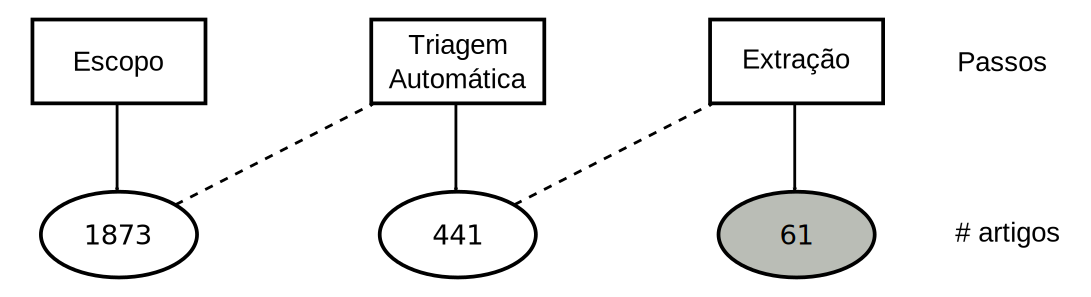
\includegraphics[scale=0.4]{imagens/revisao-literatura.png}
  \caption{Passos da revisão de literatura realizada nas conferências ASE e SCAM.}
  \label{revisao-literatura}
\end{figure}
% figura feita com base no artigo Nicolli Alves 2016, Fig 2

\subsubsection{Passo 1: Escopo}

A busca realizada nas conferências ASE e SCAM até o ano de 2015 resultou em
1873 artigos, deste total 346 artigos são do SCAM e 1527 artigos do ASE.

%Coletamos o título de cada artigo e armazenamos juntamente com o nome da
%conferência e edição onde o artigo foi publicado num arquivo do tipo ODS,
% detalhes sobre este
%arquivo pode ser encontrado no Apêndice \ref{reproducibilidade-do-estudo}.

\subsubsection{Passo 2: Triagem Automática}

O filtro executado automaticamente usando os critérios definidos na fase de
preparação reduziu o conjunto de 1873 para 441 artigos, 155 artigos do SCAM e
286 artigos do ASE, estes artigos serão inspecionados manualmente na atividade
seguinte.

\subsubsection{Passo 3: Extração}

Nesta atividade os 441 artigos foram inspecionados manualmente tendo como guia
os critérios descritos na Tabela \ref{criterios-extracao} na fase de
planejamento, selecionamos, nesta atividade, 61 artigos com publicação de
software acadêmico de análise estática

\subsection{Caracterização dos projetos de software acadêmico de análise estática}

Conforme planejado coletamos informações adicionais, descritas na Tabela
\ref{esquema-caracteristicas}, para cada projeto de software consultando
documentos de cada projeto, as informações coletadas são apresentadas, de forma
resumida, na Tabela \ref{software-table}.


\begin{longtable}{| l | l | l | l |}
\caption{Software acadêmico para análise estática.}
\label{software-table} \\
  \hhline{| l | l | l | l |}
  \hline
  \endfirsthead
  \hhline{| l | l | l | l |}
  \hline
  \textbf{Nome do software} & \textbf{Acesso} & \textbf{Código fonte} & \textbf{Distribuição} \\
  \hline
  \hhline{| l | l | l | l |}
  \endhead
  \hhline{|----|}
  \multicolumn{4}{|c|}{continua na próxima página} \\
  \hline
  \hhline{|----|} \endfoot
  \hhline{|----|} \endlastfoot
  \textbf{Nome do software} & \textbf{Acesso} & \textbf{Código fonte} & \textbf{Distribuição} \\
  \hline
    2LS &
      Gratuito &
      C++ &
      Livre \\
    AccessAnalysis &
      Gratuito &
      Java &
      Livre \\
    APIExample &
      Sem Acesso &
      - &
      - \\
    BEG &
      Sem Acesso &
      - &
      - \\
    ccJava &
      Sem Acesso &
      - &
      - \\
    CIVL &
      Gratuito &
      C &
      Livre \\
    CodeBoost &
      Gratuito &
      C &
      Livre \\
    CSL &
      Gratuito &
      C &
      Grátis \\
    CPA+ &
      Sem Acesso &
      - &
      - \\
    CSeq &
      Gratuito &
      C &
      Livre \\
    DDVerify &
      Sem Acesso &
      - &
      - \\
    Derailer &
      Gratuito &
      Ruby &
      Livre \\
    Diagnosys &
      Sem Acesso &
      - &
      - \\
    DOMPLETION &
      Gratuito &
      Javascript &
      Grátis \\
    DRC &
      Sem Acesso &
      - &
      - \\
    e-munity &
      Gratuito &
      C &
      Grátis \\
    EJB Interceptor Analyzer &
      Gratuito &
      Java &
      Grátis \\
    Error Prone &
      Gratuito &
      Java &
      Livre \\
    ESBMC &
      Sem Acesso &
      - &
      - \\
    ETXL &
      Sem Acesso &
      - &
      - \\
    FaultBuster &
      Gratuito &
      - &
      Grátis \\
    Flowgen &
      Gratuito &
      Python &
      Livre \\
    GRT &
      Sem Acesso &
      - &
      - \\
    GUIZMO &
      Gratuito &
      Java &
      Livre \\
    GumTree &
      Gratuito &
      Java &
      Livre \\
    HUSACCT &
      Gratuito &
      Java &
      Livre \\
    Indus &
      Gratuito &
      Java &
      Livre \\
    JastAdd &
      Gratuito &
      Java &
      Livre \\
    JFlow &
      Gratuito &
      Java &
      Livre \\
    JstereoCode &
      Sem Acesso &
      - &
      - \\
    Jtop &
      Sem Acesso &
      - &
      Livre \\
    Bogor/Kiasan &
      Gratuito &
      Java &
      Livre \\
    Loopfrog &
      Gratuito &
      - &
      Grátis \\
    Lotrack &
      Gratuito &
      Java &
      Grátis \\
    MPAnalyzer &
      Gratuito &
      Java &
      Grátis \\
    MSP &
      Sem Acesso &
      - &
      - \\
    mygcc &
      Gratuito &
      C &
      Livre \\
    PARSEWeb &
      Sem Acesso &
      - &
      - \\
    PAT &
      Sem Acesso &
      - &
      - \\
    PHP AiR &
      Gratuito &
      Rascal &
      Grátis \\
    protopurity &
      Gratuito &
      Javascript &
      Grátis \\
    Pseudogen &
      Gratuito &
      Python &
      Grátis \\
    PtYasm &
      Gratuito &
      Java &
      Grátis \\
    PuMoC &
      Sem Acesso &
      - &
      - \\
    PYTHIA &
      Sem Acesso &
      - &
      - \\
    ReAssert &
      Gratuito &
      Java &
      Livre \\
    Rêve &
      Sem Acesso &
      - &
      - \\
    RRFinder &
      Sem Acesso &
      - &
      - \\
    Sapid/XML &
      Sem Acesso &
      - &
      - \\
    Sonar Qube Plug-in &
      Gratuito &
      Java &
      Grátis \\
    SPARTA &
      Gratuito &
      Java &
      Grátis \\
    srcML &
      Gratuito &
      C++ &
      Livre \\
    SWAT &
      Sem Acesso &
      - &
      - \\
    TACLE &
      Gratuito &
      Java &
      Grátis \\
    TEBA &
      Gratuito &
      Perl &
      Grátis \\
    TestEra &
      Sem Acesso &
      - &
      - \\
    Vdiff &
      Sem Acesso &
      - &
      - \\
    WALA &
      Gratuito &
      Java &
      Livre \\
    Wrangler &
      Gratuito &
      Erlang &
      Livre \\
    XOgastan &
      Sem Acesso &
      - &
      - \\
  \hline
\end{longtable}



Dois artigos, entre os 61, fazem referência a um mesmo software, assim temos no
total 60 projetos de software selecionados, para cada projeto foi criado um
diretório contendo o nome do software e um arquivo chamado
\texttt{software.yml} com os dados coletados.

% }}}

% Raw results from the analysis
\section{Análise dos Dados} \label{estudo1:analise}

Coletamos 1873 artigos publicados nas conferências de Engenharia de Software
ASE e SCAM, selecionamos 61 artigos com publicação de software acadêmico de
análise estática, entre estes artigos caracterizamos 60 projetos de software,
coletamos para cada um ao menos nome e URL do projeto, e para cada projeto
informaçoes adicionais foram coletadas em fontes documentais diversas à respeito
do projeto, à seguir apresentamos a análise destes dados.

\subsection{Revisão de literatura com publicação de software de análise estática}

\subsubsection{Passo 1: Escopo}

A conferência ASE publica quase 4 vezes mais do que a conferência SCAM, a
edição com o maior número de publicações foi 2011 com 112 artigos publicados,
seguido de 2014 com 104, e 2007 com 102, a edição com o menor número foi 1996
com apenas 15 artigos publicados, A Figura \ref{artigos-por-ano} apresenta este
total distribuídos ao longo de cada edição.

\begin{figure}[h]
  \center
  \includegraphics[scale=0.65]{imagens/artigos-por-ano.png}
  \caption{Total de artigos por ano publicados nas conferências ASE e SCAM.}
  \label{artigos-por-ano}
\end{figure}


\subsubsection{Passo 2: Triagem Automática}

Para a conferência ASE até o ano de 1996 nenhum artigo foi encontrado com
ocorrência das palavras chave utilizadas no filtro, apenas a partir de 1997
temos ocorrência dos termos pesquisados nas publicações desta conferência.

\subsubsection{Passo 3: Extração}

Considerando todo o período incluído na revisão de literatura encontramos uma
média de 2 artigos por ano com publicação de software acadêmico, a Figura
\ref{artigos-com-software-por-ano} apresenta os resultados distribuídos por
ano.

\begin{figure}[h]
  \center
  \includegraphics[scale=0.65]{imagens/artigos-com-software-por-ano.png}
  \caption{Artigos com publicação de software acadêmico selecionados na revisão de literatura.}
  \label{artigos-com-software-por-ano}
\end{figure}

A revisão de literatura teve como critério primordial encontrar publicação de
software com indicação de URL para download, ainda assim, no processo de
revisão encontramos 51 projetos sem indicação de URL para download, 30 projetos
na conferência ASE e 21 projetos na conferência SCAM.

%Os 30 projetos sem indicação de URL encontrados no ASE são:
%AGENDA, Rostra, VisAXSM, Jink, AMNESIA, ISIS4J, Decor, Smack, CBFA, iMaus,
%CPPCHECKER, Tikanga, Doc2Spec, Drails, ClassSplitter, UMGAR, Secoria,
%Impendulo, BEST, DC2, WAIVE+, COPES, Ranger, ProgramCutter, Scoria, Relda,
%CONBOL, SymCrash, CodeHow, SAFEWApp.

%Os 21 projetos sem indicação de URL encontrados no SCAM são:
%ReWeb, DMS, EMBER, VADA, ADiMat, AMOEBA, JSysDG, MAGIC, SCATR, ELAN, HaRe,
%X-DEVELOP, SUDS, Goanna, Parfait, Templar, MemSafe, CAWDOR, LIBCROOS, GASR,
%PtrTracker.

% Hypothesis rejection
\section{Interpretação dos Resultados} \label{estudo1:interpretacao}

\subsection{Q1 - \EstudoUmQuestaoUm} % presença online

Dos 60 projetos de software estudados neste trabalho, 15 não tem presença
oficial online no endereço de URL informado pelos seus autores, 45 projetos estão presentes através da
URL informada de alguma forma, significando que a URL informada pelos autores
estão ativas e online. %, alguns destes projetos ...

\subsection{Q2 - \EstudoUmQuestaoDois} % download

Entre os 60 projetos selecionados 24 não estão disponível para download, ou
seja, apesar dos autores informar no estudo uma URL, indicar que o software
está disponível nesta URL para download, a URL não mais está disponível e o
software não pode ser encontrado, ou seja, 40\% dos projetos de software
acadêmico de análise estática publicados nas conferências de Engenharia de
Software ASE e SCAM não estão disponíveis.

Os demais 36 projetos, que equivalem a 60\% do conjunto total, estão
disponíveis para download e é possível obter uma cópia destes projetos na URL
indicada pelos seus autores, um resumo deste total por ano é apresentado na
Tabela \ref{available-table}.

\begin{table}[h]
\caption{Número de projetos disponível para download por ano.}
\centering
\begin{tabular}{l c c c}
  \hline
  {\bf Ano} & {\bf Total} & {\bf Disponível} & {\bf Indisponível} \\
  \hline
  2001 & 2 & 1 & 1 \\
  2003 & 3 & 1 & 2 \\
  2004 & 1 & 0 & 1 \\
  2006 & 5 & 4 & 1 \\
  2007 & 4 & 1 & 3 \\
  2008 & 2 & 1 & 1 \\
  2009 & 4 & 2 & 2 \\
  2010 & 5 & 3 & 2 \\
  2011 & 5 & 2 & 3 \\
  2012 & 6 & 2 & 4 \\
  2013 & 4 & 2 & 2 \\
  2014 & 12 & 11 & 1 \\
  2015 & 7 & 6 & 1 \\
  2016 & 4 & 4 & 0 \\
  2017 & 4 & 4 & 0 \\
  \hline
  {\bf Total} & 68 & 44 & 24 \\
  \hline
\end{tabular}
\label{available-table}
\end{table}


%Existe uma leve tendência, ao longo dos anos,  para a indisponibilidade das
%fontes informadas e páginas web.  É possível notar que, em 2006, 80\% de todos
%os softwares de análise estática publicados nas conferências ASE e SCAM ainda
%estão disponíveis.  Este número cresce em 2014, chegando a 90\%, e cai no ano
%seguinte para 85\%.  Apesar de não estar sempre crescente, e da  amostra
%pequena usada neste estudo -- apenas 60 projetos de software acadêmico, este
%leve indício confirma a afirmação de \citeonline{robles2010replicating}.

\subsection{Q3 - \EstudoUmQuestaoTres} % codigo fonte

Do conjunto de 36 projetos de software disponível para download, apenas 2 não
disponibilizam o código fonte, estão disponíveis apenas em formato binário, são
FaultBuster e Loopfrog, ambos disponibilizados gratuitamente mas apenas em
formato binário. A Tabela \ref{source-code-table} traz um resumo de quais
linguagens de programação estes softwares são escritos.

%Do conjunto de 60 projetos de software estudados, %% Joenio, coloquei aqui o tempo no PRETERITO -- revisar outras partes.
%3 não disponibilizaram seu código fonte e  %% Joenio, mudei as frases para VOZ ativa, sujeito: projeto de software.
%34 disponibilizaram o código fonte publicamente.



\begin{table}[h]
\caption{Linguagem de programação dos projetos com código fonte disponível.}
\centering
\begin{tabular}{l c}
  \hline
  {\bf Linguagem de programação} & {\bf Número de projetos} \\
  \hline
  C & 6 \\
  C++ & 2 \\
  Erlang & 1 \\
  Java & 18 \\
  Javascript & 2 \\
  Perl & 1 \\
  Python & 2 \\
  Rascal & 1 \\
  Ruby & 1 \\
  \hline
  {\bf Total} & 34 \\
  \hline
\end{tabular}
\label{source-code-table}
\end{table}



\subsection{Q4 - \EstudoUmQuestaoQuatro} % licença

Dentre os 34 projetos que disponibilizaram o código fonte, 13 não informaram
licença alguma e 19 informaram licenças de FOSS ({\it free and open source
software}), a Tabela \ref{license-table} resume as licenças utilizadas e o
número de projetos em cada uma.

\begin{table}[h]
\caption{Licenças de software dos projetos com código-fonte disponível.}
\centering
\begin{tabular}{l c c c}
  \hline
  \multirow{2}{*}{{\bf Licença de software}} & \multicolumn{3}{c}{{\bf Número de projetos}} \\
                                             & {\bf SCAM} & {\bf ASE} & {\bf Total} \\
  \hline
  Affero General Public License &
    - &
    1 &
    1 \\
  Apache License &
    1 &
    1 &
    2 \\
  BSD License &
    2 &
    2 &
    4 \\
  Eclipse Public License &
    3 &
    - &
    3 \\
  FrontEndART Software Ltd &
    1 &
    - &
    1 \\
  GNU General Public License &
    3 &
    3 &
    6 \\
  GNU Lesser General Public License &
    - &
    1 &
    1 \\
  Illinois/NCSA Open Source License &
    - &
    2 &
    2 \\
  MIT &
    2 &
    - &
    2 \\
  SAnToS Laboratory Open Academic License &
    - &
    1 &
    1 \\
  (sem licença) &
    10 &
    8 &
    18 \\
  \hline
  {\bf Total} & 22 & 19 & 41 \\
  \hline
\end{tabular}
\label{license-table}
\end{table}


Todo software com o código fonte disponível pode ser adaptado para uso pessoal
sem qualquer restrição prévia pelos seus autores, mas os 13 projetos sem
licença definida impedem eventuais cientistas a publicar suas modificações e
redistribuir qualquer melhoria sem prévia solicitação aos autores originais.

Considerando o total de 60 projetos selecionados neste estudo, apenas 32\% (19
projetos) podem ser adaptados, os demais, 68\% (41 projetos) podem ser
adaptados mas as melhorias ou correções não podem ser redistribuídas sem
autorização prévia dos autores.

\section{Ameaças à validade}

O passo de triagem automática dos artigos no processo de revisão de literatura
pode ter excluído do processo de revisão algumas publicações com software
acadêmico de análise estática, fazendo o conjunto total de projetos
selecionados escapar algum projeto, apesar disso, o estudo tem como objetivo
caaracterizar os projetos e não as conferências em sí, de forma que esta ameaça
não causa impacto nas conclusões finais do estudo.

O escopo do estudo foi reduzido ao domínio de análise estática, portanto as
conclusões e interpretações estão limitadas neste contexto, acreditamos que
outros domínios de aplicação possui características semelhantes, mas é
conhecido que o domínio de aplicação é um fator de influência relevante nas
características dos produtos de software.

A leitura dos artigos na revisão, na fase final de Extração, foi realizado
apenas pelo autor deste trabalho, é certo que poderíamos aumentar a validade
realizando a revisão em par e revisados por outros pesquisadores.

O contexto selecionado com apenas duas conferências nos leva a possibilidade de
ter resultados com viés atrelado a estes dois eventos, é possível que as
características dos projetos publicados em outras conferências da Engenharia de
Software apresentem situação diferentes.

\section{Conclusões} \label{estudo1:conclusoes}

Este estudo selecionou 60 projetos de software de análise estática de código
fonte publicados nas conferências ASE e SCAM, todos identificados com nome do
projeto e URL para download, os autores afirmam que os projetos estão
disponíveis para obtenção na URL indicada, mas os resultados da caracterização
feita mostra que apenas uma parcela destes projetos continuam disponíveis.

Entre os 60 projetos selecionados, 15 não tem qualquer presença oficial online,
estando a URL indicada pelos autores indisponível, as únicas informações
disponíveis destes 15 projetos são aquelas encontradas nos artigos onde foram
publicados.

Os outros 45 projetos com presença online através da URL informada nos artigos
9 não disponibilizam qualquer artefato relacionado ao software, apesar de ser
possível acessar a URL não é possível encontrar o software para download.

Os 36 restantes com URL disponível estão disponível para download, a maior
parte com o código fonte disponível na URL informada, 2 estão disponíveis
apenas em formato binário. Entre os projetos com código fonte disponível
uma parcela deixa explícito qual licença e de que forma o software é
distribuído.

Uma parte dos 34 projetos com código fonte disponível não informa qualquer
licença, de uso, 13 ao total, e dessa forma impedem que melhorias e correções
sejam distribuídas sem antes haver uma solicitação prévia aos autores destes
projetos. Os demais projetos, 19 utilizam licenças de software livre e dão
prévia autorização para receber melhorias em código fonte.

É conhecido que os projetos de software desenvolvidos na academia não são ainda
reconhecidos pela Ciência como cidadãos de primeira classe, mesmo quando tais
projetos são indispensáveis para a compreensão dos estudos em que foram
desenvolvidos, neste estudo mostramos que uma grande parte (40\%) de um
conjunto de projetos de software acadêmico minimamente identificados pelos seus
autores com nome e URL encontram-se hoje indisponíveis.

No entanto, nao sabemos quais fatores influenciam um projeto estar ou não
disponível, e ainda, como tais projetos são vistos por outros pesquisadores, se
são utilizados e referenciados por outros autores, assim planejamos dois
estudos para investigar tais questões, apresentados nos próximos capítulos.

%Percebemos também que existe uma grande quantidade de projetos de software
%publicados nestas duas sem indicação alguma de URL para obtenção do software,
%indicando que a ...

%detalhes sobre o formato YAML, estrutura utilizada para armazenamento e
%instalação estão documentados no Apêndice \ref{reproducibilidade-do-estudo}.

%Detalhes sobre o funcionamento do script de fitro, código fonte e instruções
%de uso podem ser consultados no Apêndice \ref{reproducibilidade-do-estudo}.

%Instruções de uso do sloccount e como ele foi utilizado neste estudo está
%documentado no Apêndice \ref{reproducibilidade-do-estudo}.

%com estas palavras num script, instalamos todas as suas
%dependências de execução, os detalhes de instalação e forma de uso deste script
%e suas dependências são documentados no Apêndice
%\ref{reproducibilidade-do-estudo}.

%% Planejamos fazer outro estudo ... 

\xchapter{Reconhecimento de software acadêmico de análise estática}
{}\label{estudo2}

Este capítulo apresenta
um estudo de caracterização do reconhecimento de software acadêmico de análise estática,
com base em informações sobre
citações formais e informais ao software %%chris: ver se formal / informal faz sentido
extraídas de um conjunto de artigos científicos publicados em periódicos ou conferências.

A seção \ref{estudo2:introducao} contextualiza o estudo
%a seção \ref{estudo2:fundamentacao} apresenta os conceitos teóricos necessários para compreensão do trabalho,
e a seção \ref{estudo2:escopo} apresenta seu objetivo e questões de pesquisa.
A seção \ref{estudo2:planejamento} apresenta o planejamento do estudo, e
as seções \ref{estudo2:preparacao} e \ref{estudo2:coleta} descrevem a preparação e execução da coleta de dados.
As seções \ref{estudo2:analise}, \ref{estudo2:interpretacao} e \ref{estudo2:ameacas}
apresentam a análise de dados, interpretação de resultados e ameaças à validade, respectivamente.
Finalmente, a seção \ref{estudo2:conclusoes} traça as conclusões do estudo.

\section{Motivação} \label{estudo2:introducao} % {{{

Um dos sintomas de 
{\it ``dysfunctional chaotic churn''} \cite{howison2015understanding}
em software acadêmico é a quantidade elevada de projetos 
com características e funcionalidades parecidas, 
e comunidades
desconectadas e paralelas.
Neste cenários, alguns projetos podem se destacar e obter o reconhecimento
de seus pares.

O desenvolvimento de sotware acadêmico é uma atividade que consome recursos
(tempo, dinheiro e atenção) e afeta a conduta da Ciência, tanto no geral como
em campos específicos. 
A colaboração no desenvolvimento destes projetos é vista
neste estudo como uma importante estratégia para lidar com o baixo orçamento
das pesquisas, bem como para mitigar os problemas do limitado tempo dos
cientistas e da alta rotatividade entre os grupos de pesquisa.

Esta estratégia de colaboração se torna especialmente interessante entre as
pesquisas da Engenharia de Software, onde, a princípio os cientistas possuem
acesso ao conhecimento e práticas necessárias para o trabalho em colaboração.
%Dessa forma, n
Neste estudo, investigamos como os projetos de software acadêmico
de análise estática são mencionados em publicações nas bases da ACM e IEEEi %e se
% há colaboração entre eles.

% }}}

%\section{Fundamentação} \label{estudo2:fundamentacao} % {{{
%\subsection{Menção}

A prática científica de citação formal entre publicações, amplamente
adotada e praticada entre cientistas de todas as áreas, não é realidade quando
se trata de artefatos digitais, como dados ou código.
Em geral, software é citado na literatura acadêmica %, na maior parte das ocorrências, de
de maneira informal: em notas de rodapé, seções de agradecimentos, e outras
seções ao longo do texto. Usualmente se faz referência ao nome, ocasionalmente
cita-se o número da versão, e raramente usa-se citação formal.
%E o reconhecimento?

Neste estudo,
O termo \textit{menção} é usado para tratar, genericamente, qualquer ocorrência de
nome de projeto de software acadêmico de análise estática em artigo científico,
incluindo tanto citação formal, quanto informal.
Uma menção pode estar associada ao uso do software no contexto de outras pesquisas,
e até mesmo a contribuições ao projeto de software acadêmico.
%extraídas de artigos científicos publicados em periódicos e conferências.

% }}}

\section{Escopo} \label{estudo2:escopo} % {{{

Quantas menções a projetos de software acadêmico de análise estática são
encontradas em publicações nas bases da ACM e IEEE? Quais são os tipos de
menções? Existe contribuição em código fonte aos projetos entre as publicações
encontradas?

O objetivo da pesquisa está definido segundo a estrutura GQM \cite{basili1994goal}.

\subsection{Definição do Objetivo}

\begin{description}
\item{\bf Objeto de estudo.} 
O objeto de estudo são projetos de software de análise estática publicados nas conferências ASE e SCAM.

\item{\bf Propósito.} 
O propósito deste estudo é caracterizar menções aos projetos.

\item{\bf Perspectiva.} 
A perspectiva considerada é a de cientista preocupado com o funcionamento do ecossistema de software acadêmico.

\item{\bf Foco de qualidade.} 
O principal aspecto de qualidade estudado é % o reconhecimento?
a contribuição ao ecossistema de software acadêmico de análise estática.

\item{\bf Contexto.} 
O estudo foi conduzido com publicações das bases ACM e IEEE.
\end{description}


O estudo realizado teve como ponto de partida
o conjunto de projetos de software identificado
no estudo sobre publicização do software acadêmico (capítulo~\ref{estudo1}).
Uma revisão da literatura nas bases da ACM e IEEE
encontrou \SearchUniqueCount \ artigos com menções ao
software acadêmico de análise estática
desse conjunto.


\subsection{Sumário da Definição}

Analisar os \textit{projetos de software acadêmico de análise estática publicados nas conferências ASE e SCAM}
com o propósito de \textit{caracterizar menções}
com respeito a \textit{contribuição ao ecossistema de software acadêmico}
na perspectiva de \textit{cientistas}
no contexto de \textit{publicações nas bases ACM e IEEE}.

\subsection{Questões de Pesquisa}

Neste estudo, três questões de pesquisa a respeito dos projetos de
software acadêmico de análise estática serão investigadas:

\newcommand{\EstudoDoisQuestaoUm}{
  Como os projetos de software acadêmico de análise estática publicados nas
  conferências ASE e SCAM são \textit{mencionados} em publicações nas bases ACM e IEEE?
}
\newcommand{\EstudoDoisQuestaoDois}{
  Os projetos de software acadêmico de análise estática publicados nas
  conferências ASE e SCAM são \textit{usados} em publicações nas bases ACM e IEEE?
}
\newcommand{\EstudoDoisQuestaoTres}{
  Os projetos de software acadêmico de análise estática publicados nas
  conferências ASE e SCAM \textit{recebem contribuições de código fonte} em publicações
  nas bases ACM e IEEE?
}

\begin{description}
  \item [Q1:] \EstudoDoisQuestaoUm
  \item [Q2:] \EstudoDoisQuestaoDois
  \item [Q3:] \EstudoDoisQuestaoTres
\end{description}

\subsection{Métricas}

Para responder às questões de pesquisas, as seguintes métricas serão usadas:

\begin{enumerate}
  \item Número de publicações nas bases ACM e IEEE com menção a projetos de
    software acadêmico de análise estática.
  \item Número de publicações nas bases ACM e IEEE com menção a uso de
    software acadêmico de análise estática.
  \item Número de publicações nas bases ACM e IEEE com menção a contribuição de
    código fonte em projetos de software acadêmico de análise estática.
\end{enumerate}

% }}}

\section{Planejamento do Estudo} \label{estudo2:planejamento} % {{{

O estudo foi realizado a partir de uma revisão de literatura nas bases ACM e
IEEE em busca de menções aos \SoftwareCount \ projetos de software acadêmico de
análise estática selecionados no Capítulo \ref{estudo1}. Um esquema de
caracterização para classificação das menções emergiu dessa revisão; 
os artigos foram então inspecionados e as menções encontradas foram classificadas segundo
este esquema.

A revisão de literatura foi organizada em quatro passos, detalhados a seguir.

\subsection{Passo 1: Busca}

Este passo teve como objetivo encontrar artigos nas bases
ACM\footnote{\url{http://dl.acm.org}} e
IEEE\footnote{\url{http://ieeexplore.ieee.org}} a partir das características
dos projetos de software acadêmico de análise estática.
As duas bases serão pesquisadas através de strings de busca previamente
elaboradas para cada um dos projetos.

A elaboração das strings deve ser realizada com o apoio dos dados já coletados
e disponíveis para cada projeto de software acadêmico, por exemplo, nome,
descrição, autores, URL, entre outros dados. Este processo de criação das
strings é realizado de maneira incremental e iterativa, iniciando por uma busca
utilizando apenas o nome do projeto, avaliando os resultados, inspecionando o
título dos artigos, refinando as strings e repetindo todo o processo até
atingir resultados dentro dos critérios desejados.

Estes critérios são definidos principalmente pelo
número de resultados obtidos na busca.
Sabemos, por experiência prática, que o número de referências a cada projeto na
literatura acadêmica não chega a casa da centena; dessa forma, o critério de
aceitação adotado para parada do processo de elaboração e refinamento das strings é
quando os resultados apresentem um número inferior ou próximo a esta realidade.

A elaboração das strings e a busca com a versão final será
realizada manualmente, usando a busca avançada dos sites das bases pesquisadas,
representadas nas Figuras \ref{advanced-search-acm} e
\ref{advanced-search-ieee}, com destaque para os campos e elementos de formulário
utilizados. É importante destacar que durante a busca na
base IEEE (Figura \ref{advanced-search-ieee}) é necessário marcar a opção {\it Full Text \& Metadata} para que a
busca considere tanto os metadados quanto o conteúdo dos artigos.

\begin{figure}[h]
  \center
  \frame{\includegraphics[scale=0.4]{imagens/advanced-search-acm.png}}
  \caption{Captura de tela da busca avançada da base ACM com destaque para (A) campo de entrada da string de busca.}
  \label{advanced-search-acm}
\end{figure}

\begin{figure}[h]
  \center
  \frame{\includegraphics[scale=0.4]{imagens/advanced-search-ieee.png}}
  \caption{Captura de tela da busca avançada da base IEEE com destaque para (A) opção de busca completa e (B) campo de entrada da string de busca.}
  \label{advanced-search-ieee}
\end{figure}

O resultado da busca final de cada projeto em cada base deve ser exportado e
copiado localmente em formato BibTeX, e ambas as bases exportam os resultados
neste formato. Os resultados finais da busca de todos os projetos serão combinados
e agregados num resultado único, sem duplicação de resultados, contendo os
metadados de todos os artigos, sem repetição.

Este resultado final, além de eliminar a duplicação de resultados, será a base
para a definição de uma identificação única para cada artigo encontrado; esta
identificação será utilizada nos próximos passos para relacionar os projetos
aos artigos através das menções encontradas. Por fim, será feito o download de cada
artigo em formato pdf para inspeção manual na etapa seguinte.

\subsection{Passo 2: Triagem}

Neste passo selecionamos os artigos relevantes para cada projeto entre os
resultados da busca realizada no passo anterior. A seleção é realizada através
de inspeção manual de cada artigo entre os resultados de cada projeto. O
critério de inclusão para a seleção dos artigos relevantes é a simples
ocorrência do nome do projeto no artigo.

Entre os resultados de cada projeto, um artigo deverá ser identificado como
relevante para o projeto caso o critério de inclusão seja satisfeito durante a
inspeção manual do artigo. Ao final deste passo, teremos, para cada projeto
de software, um conjunto de artigos identificados como relevantes que fazem
menção ao nome do projeto.

\subsection{Passo 3: Keywording}

Neste passo será criado um esquema de codificação para caracterização das
menções. O esquema é criado a partir da \textit{identificação do contexto} em que os
projetos são mencionados. Para cada menção, toma-se nota sobre como o projeto de
software é mencionado no artigo.

As notas são comentários livres descrevendo as menções encontradas no artigo
sobre um determinado software, um artigo científico pode mencionar um software
diversas vezes, de diversas formas, desde uma simples menção nos trabalhos
relacionados até uma grande contribuição ao software.

O conjunto final de todas as anotações são agrupadas e analisadas em conjunto
para definição do esquema de codificação para caracterização das menções. Este
esquema deve ser construído com o objetivo de agrupar e caracterizar os tipos
de menção encontrados para cada projeto de software em termos da contribuição
que a menção traz ao ecossistema de software daquele projeto acadêmico.

%, cada
%menção representa uma entrada em forma de contribução ao ecossistema, seja
%fazendo o projeto de software ser visível na literatura acadêmica, seja com
%contribuição direta em código ao projeto.

\subsection{Passo 4: Extração}

Neste último passo da revisão de literatura utiliza-se o esquema de codificação
para caracterização de menções criado no passo anterior para classificar as
menções de cada projeto de software encontradas nos artigos relevantes
selecionados no Passo 2: Triagem.

Para cada artigo mencionando um certo projeto de software será atribuído uma
informação indicando o tipo de menção entre as opções do esquema de codificação
para caracterização das menções.

Ao final da revisão de literatura teremos para cada projeto de software um
conjunto de artigos relevantes mencionando o software, com indicação do tipo de menção
através do esquema de codificação para caracterização de menções elaboradas no Passo 3: Keywording.

% }}}

\section{Preparação} \label{estudo2:preparacao} % {{{

Nesta seção apresentamos a preparação do estudo para a realização da coleta de
dados, incluindo a definição de arquivos e formatos de armazenamento, bem como
a implementação de scripts para coleta, análise e transformação.
A Figura \ref{estudo2-fluxograma} apresenta uma visão geral da solução adotada
e da relação entre os passos da revisão de literatura, detalhados a seguir.

\begin{figure}[h]
  \center
  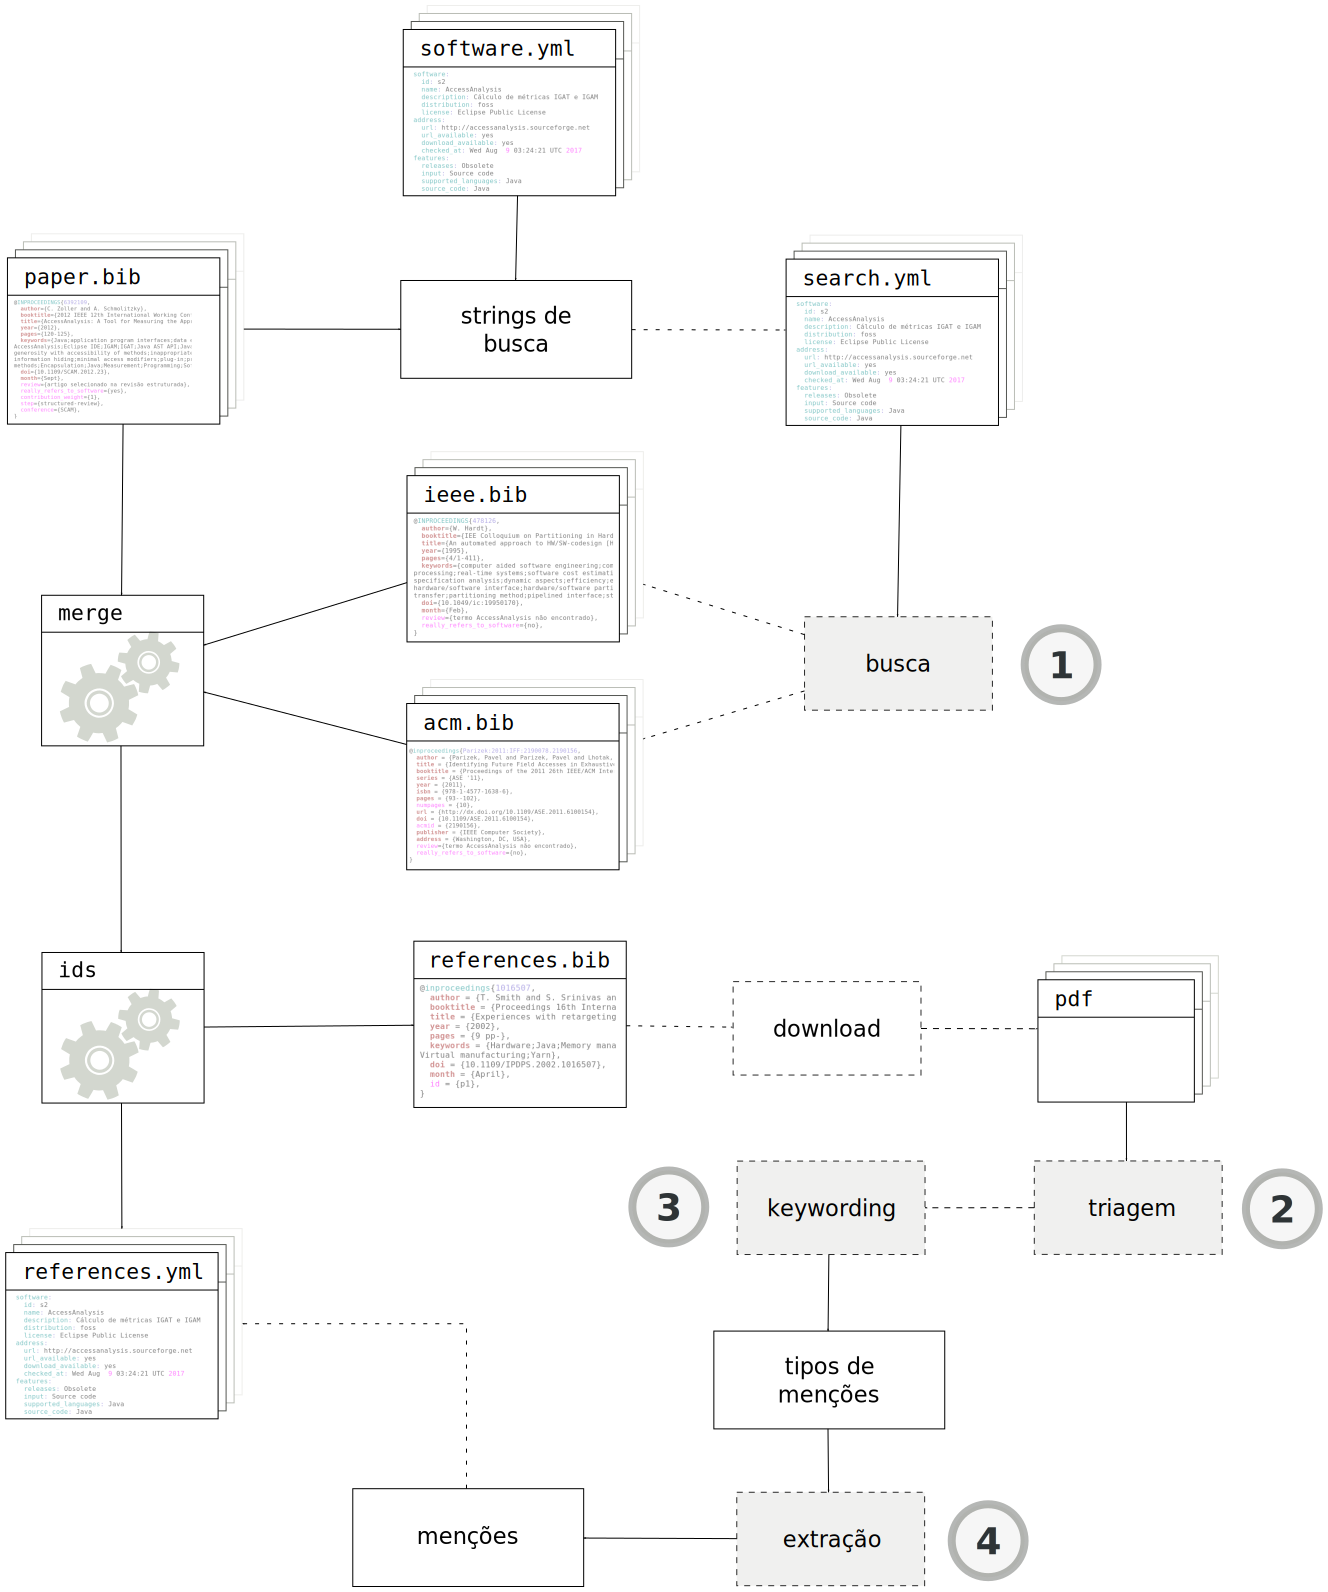
\includegraphics[scale=0.35]{imagens/estudo2-fluxograma.png}
  \caption{Fluxo de coleta, análise e transformação dos dados.}
  \label{estudo2-fluxograma}
\end{figure}

%Definimos em linhas gerais utilizar arquivos em texto plano para armazenar
%os dados coletados visando a facilidade e transparência ao acesso aos dados
%por

\subsection{Passo 1: Busca}

Seguindo o planejamento descrito na seção \ref{estudo2:planejamento} criamos as
strings de busca e as registramos nos arquivos \texttt{search.yml} de cada
projeto, este arquivo irá registrar também o número de resultados e a data de
execução da busca. A Listagem \ref{search-yml} apresenta um exemplo deste
arquivo com campos utilizados para registrar os resultados da busca.

\begin{lstlisting}[
caption={Arquivo search.yml.},
label={search-yml},
frame=single,
numbers=left
]
  acm:
    string:
    searched_at:
    results:
  ieee:
    string:
    searched_at:
    results:
\end{lstlisting}

Além deste arquivo, será criado também para cada projeto os arquivos
\texttt{acm.bib} e \texttt{ieee.bib} para armazenar os dados dos artigos
retornados pela busca. Estes dados, de todos os projetos, serão agregados no
arquivo \texttt{documents/references.bib} e identificados com
o campo \texttt{id} recebendo valores no formato \texttt{p + NÚMERO},
exemplo, \texttt{p1}, \texttt{p2}, \texttt{p3}, ..., \texttt{p806}.

Foi implementado o script \texttt{bin/ids} para automatizar a
definição deste novo campo para cada artigo, ele recebe como entrada um arquivo
no formato BibTeX e gera sequencialmente o campo \texttt{id} para cada item.

\subsection{Passo 2: Triagem}

Definimos a estrutura do arquivo \texttt{references.yml} onde será registrada a
informação dos artigos relevantes para cada projeto, a Listagem
\ref{references-yml} apresenta um exemplo deste arquivo e de sua estrutura.

\begin{lstlisting}[
caption={Arquivo references.yml.},
label={references-yml},
frame=single,
numbers=left
]
  p1:
    review:
    is_software_mentioned:
  p2:
    review:
    is_software_mentioned:
  p3:
    review:
    is_software_mentioned:
\end{lstlisting}

Em paralelo a definição deste arquivo, implementamos um mecanismo de templates,
através dos scripts \texttt{bin/cache} e \texttt{bin/render}, para criação
automática desses arquivos para cada projeto, este mecanismo de templates será
utilizado em outros pontos de estudo para automatizar e produzir documentos a
partir dos dados coletados, este mecanismo é apresentado em resumo na Figura
\ref{template-fluxograma}.

\begin{figure}[h]
  \center
  \includegraphics[scale=0.3]{imagens/template-fluxograma.png}
  \caption{Mecanismo de template para transformar dados em documentos para visualização e análise.}
  \label{template-fluxograma}
\end{figure}

%  \item[\texttt{bin/merge}]
%    Agrega os arquivos \texttt{acm.bib}, \texttt{ieee.bib} e \texttt{paper.bib}
%    de cada projeto em um único arquivo no formato BibTeX removendo
%    duplicidades dos resultados.

O script \texttt{bin/cache} cria o arquivo \texttt{cache/dataset.yml} ao
agregar todos os dados coletados de todos os projetos a partir dos arquivos
\texttt{software.yml}, \texttt{acm.bib}, \texttt{ieee.bib}, \texttt{paper.bib},
\texttt{references.yml} e \texttt{search.yml}.
O script \texttt{bin/render} lê este arquivo \texttt{cache/dataset.yml},
carrega os dados em memória e passa estes dados como parâmetro para os arquivos
templates.

\subsection{Passo 3: Keywording}

Adicionamos aos arquivos \texttt{references.yml} um novo campo para coletar o
tipo de menção feita em cada artigo aos projetos, \texttt{mention\_type}, este
campo assume um dos valores do esquema de classificação criado neste passo.

\subsection{Passo 4: Extração}

Implementamos arquivos de template para representar os dados coletados em
outros formatos para visualização e análise, incluindo documentos em formatos
CSV, Markdown e \LaTeX. Alguns destes documentos são incluídos automaticamente
neste texto.

% }}}

\section{Coleta de Dados} \label{estudo2:coleta} % {{{

Seguindo o planejamento e preparação descritos nas seções
\ref{estudo2:planejamento} e \ref{estudo2:preparacao} iniciamos a coleta dos
dados através da revisão de literatura, apresentado em resumo na Figura \ref{estudo2-revisao-literatura}.

\begin{figure}[h]
  \center
  \includegraphics[scale=0.35]{imagens/estudo2-revisao-literatura.png}
  \caption{Passos da revisão de literatura realizada nas bases ACM e IEEE.}
  \label{estudo2-revisao-literatura}
\end{figure}


\subsection{Passo 1: Busca}

A busca de todos os projetos retornou \SearchCount \ resultados,
\SearchACMCount \ na base ACM e \SearchIEEECount \ na base IEEE.
Estes resultados incluem duplicação de artigos, ou seja,
um mesmo artigo encontrado nas duas bases, ou, um mesmo artigo
encontrado em relação a mais de um projeto, dentre o resultado total.

Ao remover as duplicidades temos um conjunto de \SearchUniqueCount \ artigos
únicos.  A Tabela \ref{search-table} apresenta o total de resultados para cada
um dos projetos pesquisados, a coluna {\bf Total} inclui os artigos do arquivo
\texttt{paper.bib} e apresenta apenas resultados únicos.

\begin{longtable}{ l c c c c }
\caption{Número de resultados obtidos na busca de cada projeto de software.}
\label{search-table} \\
  \hline
  \hhline{ l c c c c |}
  \endfirsthead
  \hhline{ l c c c c |}
  \hline
   \multirow{2}{*}{\textbf{ID}} & \multirow{2}{*}{\textbf{Seleção}} & \multicolumn{2}{c}{{\bf Busca}} & \multirow{2}{*}{\textbf{Artigos únicos}} \\
   & & \textbf{ACM} & \textbf{IEEE} & \\
  \hline
  \hhline{ l c c c c |}
  \endhead
  \hhline{-----}
  \multicolumn{5}{c}{continua na próxima página} \\
  \hhline{-----} \endfoot
  \hhline{-----} \endlastfoot
   \multirow{2}{*}{\textbf{ID}} & \multirow{2}{*}{\textbf{Seleção}} & \multicolumn{2}{c}{{\bf Busca}} & \multirow{2}{*}{\textbf{Artigos únicos}} \\
   & & \textbf{ACM} & \textbf{IEEE} & \\
  \hline
\texttt{s1} & 1 & 11 & 26 & 38 \\
\texttt{s2} & 1 & 5 & 3 & 8 \\
\texttt{s3} & 1 & 10 & 6 & 15 \\
\texttt{s4} & 1 & 4 & 6 & 9 \\
\texttt{s5} & 1 & 4 & 3 & 6 \\
\texttt{s6} & 1 & 6 & 2 & 7 \\
\texttt{s7} & 1 & 16 & 9 & 25 \\
\texttt{s8} & 1 & 7 & 7 & 13 \\
\texttt{s9} & 1 & 4 & 4 & 8 \\
\texttt{s10} & 1 & 12 & 4 & 14 \\
\texttt{s11} & 1 & 2 & 2 & 3 \\
\texttt{s12} & 1 & 6 & 1 & 6 \\
\texttt{s13} & 1 & 6 & 3 & 9 \\
\texttt{s14} & 1 & 1 & 1 & 2 \\
\texttt{s15} & 1 & 15 & 4 & 16 \\
\texttt{s17} & 1 & - & 1 & 1 \\
\texttt{s16} & 1 & 1 & 4 & 5 \\
\texttt{s18} & 1 & 23 & 24 & 47 \\
\texttt{s19} & 1 & 20 & 30 & 45 \\
\texttt{s20} & 1 & 7 & 3 & 10 \\
\texttt{s21} & 1 & 1 & 3 & 3 \\
\texttt{s22} & 1 & 4 & 4 & 5 \\
\texttt{s23} & 2 & 2 & 11 & 12 \\
\texttt{s24} & 1 & - & - & 1 \\
\texttt{s25} & 1 & 20 & 17 & 34 \\
\texttt{s26} & 1 & 5 & 2 & 7 \\
\texttt{s27} & 1 & 2 & 4 & 5 \\
\texttt{s28} & 1 & 26 & 24 & 50 \\
\texttt{s29} & 1 & 11 & 5 & 15 \\
\texttt{s30} & 1 & 4 & 9 & 10 \\
\texttt{s31} & 1 & 2 & 2 & 3 \\
\texttt{s32} & 1 & 19 & 18 & 32 \\
\texttt{s33} & 1 & 3 & 3 & 5 \\
\texttt{s34} & 1 & 1 & 3 & 4 \\
\texttt{s35} & 1 & 2 & 1 & 2 \\
\texttt{s36} & 1 & 17 & 20 & 34 \\
\texttt{s37} & 1 & 2 & 5 & 7 \\
\texttt{s38} & 1 & 29 & 20 & 42 \\
\texttt{s39} & 1 & 3 & 10 & 11 \\
\texttt{s40} & 1 & 3 & 8 & 11 \\
\texttt{s41} & 1 & - & - & 1 \\
\texttt{s42} & 1 & 1 & 4 & 5 \\
\texttt{s43} & 2 & - & 2 & 2 \\
\texttt{s44} & 1 & 3 & 1 & 3 \\
\texttt{s45} & 1 & 5 & 10 & 14 \\
\texttt{s46} & 1 & 16 & 12 & 24 \\
\texttt{s47} & 1 & 6 & 7 & 13 \\
\texttt{s48} & 1 & 3 & 2 & 4 \\
\texttt{s49} & 1 & 1 & 4 & 5 \\
\texttt{s50} & 1 & 1 & 1 & 2 \\
\texttt{s51} & 1 & 2 & 5 & 7 \\
\texttt{s52} & 1 & 9 & 34 & 41 \\
\texttt{s53} & 1 & 10 & 5 & 13 \\
\texttt{s54} & 1 & 2 & 2 & 4 \\
\texttt{s55} & 1 & 3 & 8 & 12 \\
\texttt{s56} & 1 & 23 & 21 & 38 \\
\texttt{s57} & 1 & 4 & 6 & 8 \\
\texttt{s58} & 1 & 8 & 4 & 11 \\
\texttt{s59} & 1 & 25 & 12 & 36 \\
\texttt{s60} & 1 & - & 7 & 7 \\
\texttt{{\bf Média}} & {\bf 1.0} & {\bf 7.3} & {\bf 7.7} & {\bf 13.8} \\
\texttt{{\bf Total}} & {\bf 62} & {\bf 438} & {\bf 459} & {\bf 830} \\
\end{longtable}


\subsection{Passo 2: Triagem}

Os \SearchUniqueCount \ artigos foram inspecionados em busca de menções aos
projetos de software, encontramos \ScreeningCount \ menções entre
\ScreeningUniqueCount \ artigos.
Alguns projetos de software possui nomes comuns que foram encontrados nos
artigos mas não faziam referencia ao software, em alguns casos os nomes
apareciam em fórmulas matemáticas ou como parte do texto em contextos não
relacionados ao projeto.

A Figura \ref{screenshot-paper-p148-2ls} apresenta um destes casos, o nome do
projeto \texttt{s1} (2LS) foi encontrado no artigo \texttt{p148} (Statistical
Design Framework of Submicron Flip-Flop Circuits Considering Process
Variations) num contexto sem relação alguma com o projeto em sí.

\begin{figure}[h]
  \center
  \frame{\includegraphics[scale=0.45]{imagens/screenshot-paper-p148-2ls.png}}
  \caption{Exemplo de ocorrencia do nome do projeto de software em fórmula matemática.}
  \label{screenshot-paper-p148-2ls}
\end{figure}

Ao final da triagem temos, para cada projeto, um conjunto de artigos que de
fato mencionam o software, sem ainda caracterizar o tipo de menção.

\subsection{Passo 3: Keywording}

A anotação de cada uma das \ScreeningCount \ menções foram analisadas e o
esquema para caracterização foi criado com três valores distintos indicando o
nível de contribuição da menção ao ecossistema de software do projeto,
apresentados na Tabela \ref{esquema-de-mencao}.

\begin{table}[h]
\caption{Esquema para classificação de menções aos projetos software acadêmico.}
\centering
\begin{tabular}{ l p{10cm} }
  \hline
  Tipo de menção           & Explicação \\
  \hline
  Cita      & É o mesmo artigo selecionado em \texttt{paper.bib} (artigo com ``mesmo'' conteúdo publicado na ``mesma'' época); Descreve o software; Menciona o software numa tabela com outros, classifica, cita como exemplo; Menciona em trabalhos relacionados ou em trabalhos futuros. \\
  Usa       & Avalia ou caracteriza o software; Usa para coleta ou análise de dados; Usa como objeto de estudo; Usa o software como parte de uma solução, implementação, etc; Cria um software derivado sem disponibilizar as contribuições. \\
  Contribui & Contribuição inicial publicando o software; Refatora o software; Abre o código de um software que antes era código fechado; Contribuição em código fonte; Extende o software; Integra o software a outros sistemas, formatos de entrada/saída ou APIs; Implementa parte do software em outro projeto e compara resultados. \\
  \hline
\end{tabular}
\label{esquema-de-mencao}
\end{table}

\subsection{Passo 4: Extração}

A partir do esquema para caracterização das menções coletamos os valores
assumindo um dos valores da Tabela \ref{esquema-de-mencao}, encontramos
\CiteCount \ menções do tipo Cita, \UseCount \ menções do tipo Usa e
\ContributeCount \ menções do tipo Contribui. Estes dados são
apresentados em resumo na Tabela \ref{mentions-table}.

\begin{longtable}{ l c c c c | l c c c c }
\caption{Número de menções por tipo.}
\label{mentions-table} \\
  \hline
  \hhline{ l c c c c | l c c c c |}
  \endfirsthead
  \hhline{ l c c c c | l c c c c |}
  \hline
   \multirow{2}{*}{\textbf{ID}} & \multicolumn{3}{c}{{\bf Menções}} & \multirow{2}{*}{\textbf{Total}} & \multirow{2}{*}{\textbf{ID}} & \multicolumn{3}{c}{{\bf Menções}} & \multirow{2}{*}{\textbf{Total}} \\
   & \textbf{Cita} & \textbf{Usa} & \textbf{Contribui} & & & \textbf{Cita} & \textbf{Usa} & \textbf{Contribui} & \\
  \hline
  \hhline{ l c c c c | l c c c c |}
  \endhead
  \hhline{-----|-----}
  \multicolumn{10}{c}{continua na próxima página} \\
  \hhline{-----|-----} \endfoot
  \hhline{-----|-----} \endlastfoot
   \multirow{2}{*}{\textbf{ID}} & \multicolumn{3}{c}{{\bf Menções}} & \multirow{2}{*}{\textbf{Total}} & \multirow{2}{*}{\textbf{ID}} & \multicolumn{3}{c}{{\bf Menções}} & \multirow{2}{*}{\textbf{Total}} \\
   & \textbf{Cita} & \textbf{Usa} & \textbf{Contribui} & & & \textbf{Cita} & \textbf{Usa} & \textbf{Contribui} & \\
  \hline
s1 & - & - & 1 & 1 & s32 & 8 & - & 6 & 14 \\
s2 & 1 & - & 1 & 2 & s33 & 2 & 2 & 1 & 5 \\
s3 & 3 & - & 1 & 4 & s34 & 1 & - & 1 & 2 \\
s4 & 4 & 3 & 2 & 9 & s35 & - & - & 1 & 1 \\
s5 & 2 & - & 3 & 5 & s36 & 1 & - & 1 & 2 \\
s6 & 4 & - & 1 & 5 & s37 & 3 & 1 & 3 & 7 \\
s7 & 9 & - & 1 & 10 & s38 & 17 & - & 1 & 18 \\
s8 & 3 & 1 & 2 & 6 & s39 & 1 & - & 1 & 2 \\
s9 & - & - & 5 & 5 & s40 & 1 & 5 & 3 & 9 \\
s10 & 1 & 2 & 2 & 5 & s41 & - & - & 1 & 1 \\
s11 & 2 & - & 1 & 3 & s42 & - & - & 1 & 1 \\
s12 & 1 & - & 1 & 2 & s43 & - & - & 2 & 2 \\
s13 & - & - & 1 & 1 & s44 & 1 & - & 1 & 2 \\
s14 & 1 & - & 1 & 2 & s45 & - & - & 2 & 2 \\
s15 & 4 & - & 1 & 5 & s46 & 9 & 3 & 1 & 13 \\
s17 & - & - & 1 & 1 & s47 & - & - & 1 & 1 \\
s16 & 1 & 1 & 2 & 4 & s48 & 1 & - & 1 & 2 \\
s18 & - & 1 & 1 & 2 & s49 & 1 & 2 & 2 & 5 \\
s19 & 14 & 18 & 8 & 40 & s50 & - & - & 1 & 1 \\
s20 & - & - & 1 & 1 & s51 & 1 & 2 & 1 & 4 \\
s21 & - & - & 1 & 1 & s52 & 14 & 23 & 3 & 40 \\
s22 & 2 & - & 1 & 3 & s53 & 1 & 2 & 1 & 4 \\
s23 & 3 & 2 & 3 & 8 & s54 & 1 & 1 & 1 & 3 \\
s24 & - & - & 1 & 1 & s55 & - & - & 1 & 1 \\
s25 & 5 & 10 & 4 & 19 & s56 & 15 & 5 & 1 & 21 \\
s26 & 3 & 2 & 2 & 7 & s57 & 4 & - & 1 & 5 \\
s27 & - & 2 & 1 & 3 & s58 & 5 & 5 & 1 & 11 \\
s28 & 22 & 14 & 4 & 40 & s59 & 16 & 10 & 7 & 33 \\
s29 & 5 & 1 & 1 & 7 & s60 & 4 & - & 1 & 5 \\
s30 & 2 & 5 & 1 & 8 & {\bf Média} & {\bf 3.3} & {\bf 2.1} & {\bf 1.8} & {\bf 7.2} \\
s31 & - & 1 & 1 & 2 & {\bf Total} & {\bf 199} & {\bf 124} & {\bf 106} & {\bf 429} \\
\end{longtable}


É importante lembrar que as menções do tipo Contribui incluem os artigos
selecionados no arquivo \texttt{paper.bib}, independente de terem sido
encontrados na busca das bases ACM e IEEE.

% }}}

\section{Análise dos Dados} \label{estudo2:analise} % {{{

Dados de \SoftwareCount \ projetos desenvolvidos e publicados na literatura
acadêmica de Engenharia de Software, informações sobre diversas formas de
menção ao nome destes projetos, \ScreeningUniqueCount \ artigos distintos
encontrados nas bases ACM e IEEE mencionando estes projetos.

\subsection{Passo 1: Busca}

A busca nas bases ACM e IEEE retornou uma média de \SearchUniqueMean \ artigos
por projeto. Os projetos \texttt{s24} (GUIZMO) e \texttt{s41} (protopurity)
não foram encontrados em nenhuma das bases.
Os projetos \texttt{s17} (e-munity), \texttt{s43} (PtYasm) e \texttt{s60} (XOgastan)
não foram encontrados na base ACM.

Entre os projetos com resultados acima da média a maior parte está disponível
para download, 11 com acesso e 7 sem acesso.  Entre os projetos com resultados
abaixo da média, 25 está disponível para download e apenas 16 não estão
disponíveis.

%projetos com resultado da busca acima da média
% resultados  acesso
% s1  38      s
% s3  15      n
% s7  25      s
% s10 14      s
% s15 16      n
% s18 47      s
% s19 45      n
% s25 34      s
% s28 50      s
% s29 15      s
% s32 32      s
% s36 34      n
% s38 42      n
% s45 14      n
% s46 24      s
% s52 41      s
% s56 38      n
% s59 36      s
% s = 11
% n = 7

%projetos com resultado da busca abaixo da média
%resultados acesso
%s2  8      s
%s4  9      n
%s5  6      n
%s6  7      s
%s8  13     s
%s9  8      n
%s11 3      n
%s12 6      s
%s13 9      n
%s14 2      s
%s16 5      s
%s17 1      s
%s20 10     n
%s21 3      s
%s22 5      s
%s23 12     n
%s24 1      s
%s26 7      s
%s27 5      s
%s30 10     n
%s31 3      n
%s33 5      s
%s34 4      s
%s35 2      s
%s37 7      s
%s39 11     n
%s40 11     s
%s41 1      s
%s42 5      s
%s43 2      s
%s44 3      n
%s48 4      n
%s49 5      n
%s50 2      s
%s51 7      s
%s53 13     n
%s54 4      s
%s55 12     s
%s57 8      n
%s58 11     s
%s60 7      n

\subsection{Passo 2: Triagem}

Entre os resultados da busca apenas 51\% dos artigos são relevantes e fazem
menção aos projetos. Numa média de \ScreeningUniqueMean \ artigos por projeto
e \ScreeningMean \ menções por projeto.

Entre os projetos com menções acima da média, 9 estão disponíveis para download
e 6 não estão disponíveis, entre os projetos com menções abaixo da média, 25
possuem download disponível e 20 não.

% acima da média de menções
%          acesso
%s4  = 9   n
%s7  = 10  s
%s19 = 40  n
%s23 = 8   n
%s25 = 19  s
%s28 = 40  s
%s30 = 8   n
%s32 = 14  s
%s38 = 18  n
%s40 = 9   s
%s46 = 13  s
%s52 = 40  s
%s56 = 21  n
%s58 = 11  s
%s59 = 33  s

% abaixo da média de menções
%         acesso
%s1  = 1  s
%s2  = 2  s
%s3  = 4  n
%s5  = 5  n
%s6  = 5  s
%s8  = 6  s
%s9  = 5  n
%s10 = 5  s
%s11 = 3  n
%s12 = 2  s
%s13 = 1  n
%s14 = 2  s
%s15 = 5  n
%s16 = 4  n
%s17 = 1  s
%s18 = 2  s
%s20 = 1  n
%s21 = 1  s
%s22 = 3  s
%s24 = 1  s
%s26 = 7  s
%s27 = 3  s
%s29 = 7  s
%s31 = 2  n
%s33 = 5  s
%s34 = 2  s
%s35 = 1  s
%s36 = 2  n
%s37 = 7  s
%s39 = 2  n
%s41 = 1  s
%s43 = 2  s
%s44 = 2  n
%s45 = 2  n
%s47 = 1  n
%s48 = 2  n
%s49 = 5  n
%s50 = 1  s
%s51 = 4  s
%s53 = 4  n
%s54 = 3  s
%s55 = 1  s
%s57 = 5  n
%s60 = 5  n

\subsection{Passo 3: Keywording}

\CiteCount \ Cita,
\UseCount \ Usa e
\ContributeCount \ Contribui.

\subsection{Passo 4: Extração}

Entre os \SoftwareCount \ projetos, \SoftwareNotMentionedCount \ projetos
(\texttt{s1}, \texttt{s13}, \texttt{s17}, \texttt{s20}, \texttt{s21}, \texttt{s24}, \texttt{s35}, \texttt{s41}, \texttt{s42}, \texttt{s43}, \texttt{s47}, \texttt{s50}, \texttt{s55}
) não foram encontrados em menções
após a publicação inicial, sendo a única publicação aquela localizada no
arquivo \texttt{paper.bib}, referente a seleção do software no estudo
apresentado no Capítulo \ref{estudo1}.

Os demais \MentionsStudyDois \ projetos são mencionados em publicações nas
bases ACM e IEEE, deste grupo apenas \ContributeStudyDoisSoftware \ projetos
(\texttt{s10}, \texttt{s16}, \texttt{s19}, \texttt{s23}, \texttt{s25}, \texttt{s26}, \texttt{s28}, \texttt{s32}, \texttt{s37}, \texttt{s4}, \texttt{s40}, \texttt{s45}, \texttt{s49}, \texttt{s5}, \texttt{s52}, \texttt{s59}, \texttt{s67}, \texttt{s8}, \texttt{s9}
) recebem contribuições através de
\ContributeStudyDoisCount \ menções.

A Figura \ref{mentions-timeline} apresenta uma visualização da linha do tempo
de cada software em relação a menções encontradas nas bases ACM e IEEE através
da revisão de literatura.

\begin{figure}[h]
  \center
  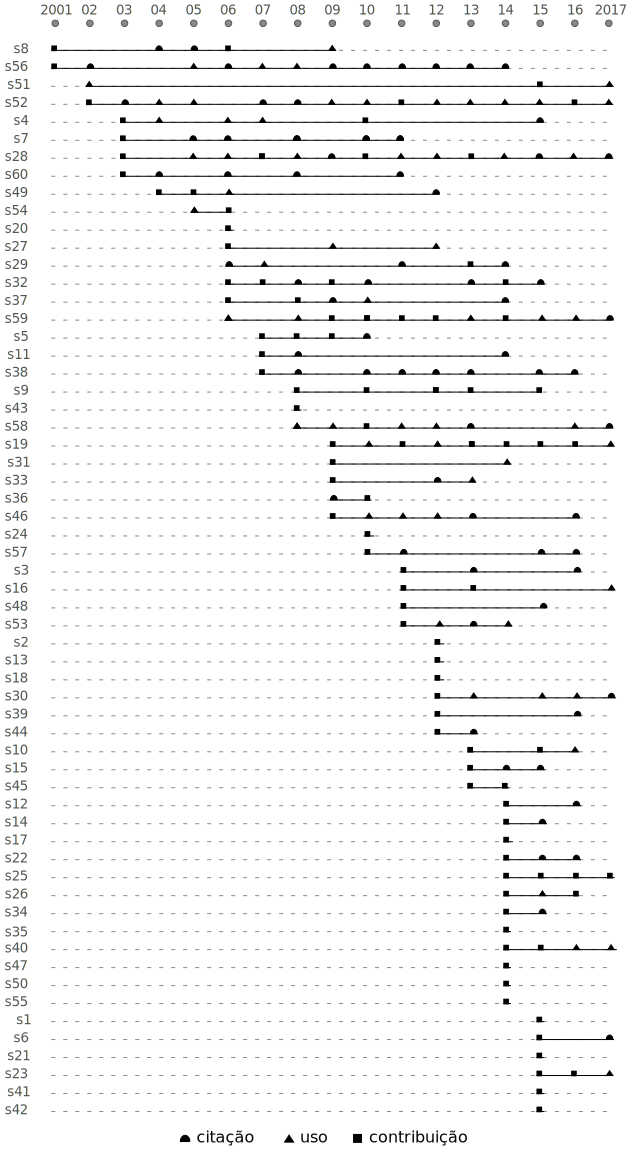
\includegraphics[scale=0.6]{imagens/mentions-timeline.png}
  \caption{Linha do tempo de menções (uso e contribuição) aos projetos nas bases ACM e IEEE.}
  \label{mentions-timeline}
\end{figure}

% }}}

\section{Interpretação dos Resultados} \label{estudo2:interpretacao} % {{{

\subsection{Q1 - \EstudoDoisQuestaoUm}

Os \SoftwareCount \ projetos de software acadêmico de análise estática
publicados nas conferências ASE e SCAM são mencionados \ScreeningCount \ vezes
em \ScreeningUniqueCount \ artigos distintos, estas menções foram encontradas
em buscas nas bases ACM e IEEE realizadas entre os meses de Julho e Agosto de
2017.

Entre todas as menções emergiu três tipos distintos em relação ao nível de
contribuição ao ecossistema dos projetos, Cita, Usa e Contribui. A maior parte
das menções encontradas é do tipo Cita (\CiteCount \ menções), em seguida
o tipo de menção Usa com \UseCount \ ocorrências, e por fim, com menor número,
o tipo de menção Contribui com \ContributeCount \ ocorrências.

\subsection{Q2 - \EstudoDoisQuestaoDois}

Encontramos \UseCount \ menções usando os projetos como apoio metodológico para
coleta ou análise de dados, como objeto de estudo, ou como ponto de partida
para implementação de outras soluções de pesquisa.

Estas menções do tipo Uso estão associadas a 26 dos \SoftwareCount \ projetos
de software, indicando que menos da metade dos projetos de software acadêmico
de análise estática publicados nas conferências ASE e SCAM são utilizados em
pesquisas nas bases ACM e IEEE.

\subsection{Q3 - \EstudoDoisQuestaoTres}

Encontramos \ContributeCount \ menções contribuindo com os projetos, este total
inclui os artigos publicando os projetos de software pela primeira vez, ou
seja, inclui os artigos que deram origem ao conjunto de \SoftwareCount \
projetos de software registrados nos arquivos \texttt{paper.bib}.

Ao analisar apenas contribuições posteriores a publicação inicial
do projeto, ou seja, artigos e estudos contribuindo com código
fonte aos projetos após a sua publicação inicial, encontramos
\ContributeStudyDoisCount \ menções a um conjunto de
\ContributeStudyDoisSoftware \ projetos de software.

Ou seja, apenas 28\% dos projetos (\texttt{s10}, \texttt{s16}, \texttt{s19}, \texttt{s23}, \texttt{s25}, \texttt{s26}, \texttt{s28}, \texttt{s32}, \texttt{s37}, \texttt{s4}, \texttt{s40}, \texttt{s45}, \texttt{s49}, \texttt{s5}, \texttt{s52}, \texttt{s59}, \texttt{s67}, \texttt{s8}, \texttt{s9}
)
recebem contribuição em código fonte de estudos após a publicação inicial, ao
menos entre estudos encontrados nas bases ACM e IEEE.

%O GRT recebe uma grande contribuição além da publicação inicial criando o projeto,
%é o único, todos os outros recebem contribuições de peso apenas na criação, ou seja,
%no paper original publicando o projeto pela primeira vez.

%Os projetos tiveram contribuições em código em publicações posteriores aos
%artigos inicias publicando o software?

%Quantos autores novos além dos autores originais/iniciais do projeto
%foram encontrados contribuindo com os projetos?

%

\begin{longtable}{ l *{17}{c} }
\caption{Número de publicações mencionando contribuição por ano (de 2001 até 2017).}
\label{contributors-table} \\
  \hline
  \hhline{ l *{17}{c} |}
  \endfirsthead
  \hhline{ l *{17}{c} |}
  \hline
  \textbf{Projeto} & 01 & 02 & 03 & 04 & 05 & 06 & 07 & 08 & 09 & 10 & 11 & 12 & 13 & 14 & 15 & 16 & 17 \\
  \hline
  \hhline{ l *{17}{c} |}
  \endhead
  \hhline{------------------}
  \multicolumn{17}{c}{continua na próxima página} \\
  \hhline{------------------} \endfoot
  \hhline{------------------} \endlastfoot
  \textbf{Projeto} & 01 & 02 & 03 & 04 & 05 & 06 & 07 & 08 & 09 & 10 & 11 & 12 & 13 & 14 & 15 & 16 & 17 \\
  \hline
    2LS &
      - &
      - &
      - &
      - &
      - &
      - &
      - &
      - &
      - &
      - &
      - &
      - &
      - &
      - &
      c &
      - &
      - \\
    AccessAnalysis &
      - &
      - &
      - &
      - &
      - &
      - &
      - &
      - &
      - &
      - &
      - &
      c &
      - &
      - &
      - &
      - &
      - \\
    APIExample &
      - &
      - &
      - &
      - &
      - &
      - &
      - &
      - &
      - &
      - &
      c &
      - &
      m &
      - &
      - &
      m &
      - \\
    BEG &
      - &
      - &
      c &
      u &
      - &
      u &
      u &
      - &
      - &
      c &
      - &
      - &
      - &
      - &
      m &
      - &
      - \\
    ccJava &
      - &
      - &
      - &
      - &
      - &
      - &
      c &
      c &
      c &
      c &
      - &
      - &
      - &
      - &
      - &
      - &
      - \\
    CIVL &
      - &
      - &
      - &
      - &
      - &
      - &
      - &
      - &
      - &
      - &
      - &
      - &
      - &
      - &
      c &
      - &
      m \\
    CodeBoost &
      - &
      - &
      c &
      - &
      m &
      m &
      - &
      m &
      m &
      m &
      m &
      m &
      m &
      - &
      m &
      - &
      - \\
    CSL &
      c &
      - &
      - &
      m &
      m &
      c &
      - &
      - &
      u &
      - &
      - &
      - &
      - &
      - &
      - &
      - &
      - \\
    CPA+ &
      - &
      - &
      - &
      - &
      - &
      - &
      - &
      c &
      - &
      c &
      - &
      c &
      c &
      - &
      c &
      - &
      - \\
    CSeq &
      - &
      - &
      - &
      - &
      - &
      - &
      - &
      - &
      - &
      - &
      - &
      - &
      c &
      - &
      c &
      u &
      - \\
    DDVerify &
      - &
      - &
      - &
      - &
      - &
      - &
      c &
      m &
      - &
      - &
      - &
      - &
      - &
      m &
      - &
      - &
      - \\
    Derailer &
      - &
      - &
      - &
      - &
      - &
      - &
      - &
      - &
      - &
      - &
      - &
      - &
      - &
      c &
      - &
      m &
      - \\
    Diagnosys &
      - &
      - &
      - &
      - &
      - &
      - &
      - &
      - &
      - &
      - &
      - &
      c &
      - &
      - &
      - &
      - &
      - \\
    DOMPLETION &
      - &
      - &
      - &
      - &
      - &
      - &
      - &
      - &
      - &
      - &
      - &
      - &
      - &
      c &
      m &
      - &
      - \\
    DRC &
      - &
      - &
      - &
      - &
      - &
      - &
      - &
      - &
      - &
      - &
      - &
      - &
      c &
      m &
      m &
      - &
      - \\
    e-munity &
      - &
      - &
      - &
      - &
      - &
      - &
      - &
      - &
      - &
      - &
      - &
      - &
      - &
      c &
      - &
      - &
      - \\
    EJB &
      - &
      - &
      - &
      - &
      - &
      - &
      - &
      - &
      - &
      - &
      c &
      - &
      m &
      - &
      - &
      - &
      u \\
    Error Prone &
      - &
      - &
      - &
      - &
      - &
      - &
      - &
      - &
      - &
      - &
      - &
      c &
      - &
      - &
      u &
      - &
      - \\
    ESBMC &
      - &
      - &
      - &
      - &
      - &
      - &
      - &
      - &
      c &
      u &
      c &
      u &
      c &
      c &
      c &
      c &
      u \\
    ETXL &
      - &
      - &
      - &
      - &
      - &
      c &
      - &
      - &
      - &
      - &
      - &
      - &
      - &
      - &
      - &
      - &
      - \\
    FaultBuster &
      - &
      - &
      - &
      - &
      - &
      - &
      - &
      - &
      - &
      - &
      - &
      - &
      - &
      - &
      c &
      - &
      - \\
    Flowgen &
      - &
      - &
      - &
      - &
      - &
      - &
      - &
      - &
      - &
      - &
      - &
      - &
      - &
      c &
      m &
      m &
      - \\
    GRT &
      - &
      - &
      - &
      - &
      - &
      - &
      - &
      - &
      - &
      - &
      - &
      - &
      - &
      m &
      c &
      c &
      u \\
    GUIZMO &
      - &
      - &
      - &
      - &
      - &
      - &
      - &
      - &
      - &
      c &
      - &
      - &
      - &
      - &
      - &
      - &
      - \\
    GumTree &
      - &
      - &
      - &
      - &
      - &
      - &
      - &
      - &
      - &
      - &
      - &
      - &
      - &
      c &
      u &
      u &
      c \\
    HUSACCT &
      - &
      - &
      - &
      - &
      - &
      - &
      - &
      - &
      - &
      - &
      - &
      - &
      - &
      c &
      u &
      c &
      - \\
    Indus &
      - &
      - &
      - &
      - &
      - &
      c &
      - &
      - &
      u &
      - &
      - &
      u &
      - &
      - &
      - &
      - &
      - \\
    JastAdd &
      - &
      - &
      m &
      - &
      u &
      u &
      c &
      c &
      m &
      c &
      u &
      u &
      c &
      u &
      m &
      u &
      m \\
    JFlow &
      - &
      - &
      - &
      - &
      - &
      m &
      u &
      - &
      - &
      - &
      m &
      - &
      c &
      m &
      - &
      - &
      - \\
    JstereoCode &
      - &
      - &
      - &
      - &
      - &
      - &
      - &
      - &
      - &
      - &
      - &
      c &
      u &
      - &
      u &
      u &
      m \\
    Jtop &
      - &
      - &
      - &
      - &
      - &
      - &
      - &
      - &
      c &
      - &
      - &
      - &
      - &
      u &
      - &
      - &
      - \\
    Bogor/Kiasan &
      - &
      - &
      - &
      - &
      - &
      c &
      c &
      m &
      c &
      m &
      - &
      - &
      m &
      c &
      m &
      - &
      - \\
    Loopfrog &
      - &
      - &
      - &
      - &
      - &
      - &
      - &
      - &
      c &
      - &
      - &
      m &
      u &
      - &
      - &
      - &
      - \\
    Lotrack &
      - &
      - &
      - &
      - &
      - &
      - &
      - &
      - &
      - &
      - &
      - &
      - &
      - &
      c &
      m &
      - &
      - \\
    MPAnalyzer &
      - &
      - &
      - &
      - &
      - &
      - &
      - &
      - &
      - &
      - &
      - &
      - &
      - &
      c &
      - &
      - &
      - \\
    MSP &
      - &
      - &
      - &
      - &
      - &
      - &
      - &
      - &
      m &
      c &
      - &
      - &
      - &
      - &
      - &
      - &
      - \\
    mygcc &
      - &
      - &
      - &
      - &
      - &
      c &
      - &
      c &
      m &
      u &
      - &
      - &
      - &
      m &
      - &
      - &
      - \\
    PARSEWeb &
      - &
      - &
      - &
      - &
      - &
      - &
      c &
      u &
      - &
      m &
      m &
      m &
      m &
      - &
      m &
      m &
      - \\
    PAT &
      - &
      - &
      - &
      - &
      - &
      - &
      - &
      - &
      - &
      - &
      - &
      c &
      - &
      - &
      - &
      m &
      m \\
    PHP AiR &
      - &
      - &
      - &
      - &
      - &
      - &
      - &
      - &
      - &
      - &
      - &
      - &
      - &
      c &
      c &
      u &
      u \\
    protopurity &
      - &
      - &
      - &
      - &
      - &
      - &
      - &
      - &
      - &
      - &
      - &
      - &
      - &
      - &
      c &
      - &
      - \\
    Pseudogen &
      - &
      - &
      - &
      - &
      - &
      - &
      - &
      - &
      - &
      - &
      - &
      - &
      - &
      - &
      c &
      - &
      - \\
    PtYasm &
      - &
      - &
      - &
      - &
      - &
      - &
      - &
      c &
      - &
      - &
      - &
      - &
      - &
      - &
      - &
      - &
      - \\
    PuMoC &
      - &
      - &
      - &
      - &
      - &
      - &
      - &
      - &
      - &
      - &
      - &
      c &
      m &
      - &
      - &
      - &
      - \\
    PYTHIA &
      - &
      - &
      - &
      - &
      - &
      - &
      - &
      - &
      - &
      - &
      - &
      - &
      c &
      c &
      - &
      - &
      - \\
    ReAssert &
      - &
      - &
      - &
      - &
      - &
      - &
      - &
      - &
      c &
      u &
      u &
      u &
      m &
      - &
      - &
      m &
      - \\
    Rêve &
      - &
      - &
      - &
      - &
      - &
      - &
      - &
      - &
      - &
      - &
      - &
      - &
      - &
      c &
      - &
      - &
      - \\
    RRFinder &
      - &
      - &
      - &
      - &
      - &
      - &
      - &
      - &
      - &
      - &
      c &
      - &
      - &
      m &
      m &
      - &
      - \\
    Sapid/XML &
      - &
      - &
      - &
      c &
      c &
      u &
      - &
      - &
      - &
      - &
      - &
      m &
      - &
      - &
      - &
      - &
      - \\
    Sonar Qube Plug-in &
      - &
      - &
      - &
      - &
      - &
      - &
      - &
      - &
      - &
      - &
      - &
      - &
      - &
      c &
      - &
      - &
      - \\
    SPARTA &
      - &
      u &
      - &
      - &
      - &
      - &
      - &
      - &
      - &
      - &
      - &
      - &
      - &
      - &
      c &
      - &
      u \\
    srcML &
      - &
      m &
      m &
      u &
      u &
      - &
      m &
      m &
      u &
      u &
      c &
      u &
      u &
      u &
      u &
      c &
      u \\
    SWAT &
      - &
      - &
      - &
      - &
      - &
      - &
      - &
      - &
      - &
      - &
      c &
      u &
      m &
      u &
      - &
      - &
      - \\
    TACLE &
      - &
      - &
      - &
      - &
      u &
      c &
      - &
      - &
      - &
      - &
      - &
      - &
      - &
      - &
      - &
      - &
      - \\
    TEBA &
      - &
      - &
      - &
      - &
      - &
      - &
      - &
      - &
      - &
      - &
      - &
      - &
      - &
      c &
      - &
      - &
      - \\
    TestEra &
      c &
      m &
      - &
      u &
      m &
      m &
      u &
      u &
      m &
      m &
      m &
      m &
      m &
      m &
      - &
      - &
      - \\
    Vdiff &
      - &
      - &
      - &
      - &
      - &
      - &
      - &
      - &
      - &
      c &
      m &
      - &
      - &
      - &
      m &
      m &
      - \\
    WALA &
      - &
      - &
      - &
      - &
      - &
      - &
      - &
      u &
      u &
      c &
      u &
      u &
      m &
      - &
      - &
      u &
      m \\
    Wrangler &
      - &
      - &
      - &
      - &
      - &
      u &
      - &
      u &
      c &
      c &
      c &
      c &
      u &
      c &
      u &
      u &
      m \\
    XOgastan &
      - &
      - &
      c &
      m &
      - &
      m &
      - &
      m &
      - &
      - &
      m &
      - &
      - &
      - &
      - &
      - &
      - \\
  \hline
\end{longtable}



%A comparação entre os nomes do autores passou antes pela normalização
%no formato de representação, visto que cada artigo utiliza um formato
%de nome diferente, transformamos, por exemplo, ``Bajaj, Kon'' em ``Bajaj K.'',
%``Costa, Kim A.'' em ``Costa K. A.'', ``Rajan, Sreeranga P.'' em ``Rajan S. P.'',
%``Pol, Jaco van de'' em ``Pol J. van de'', ``Zijiang Yang'' em ``Yang Z.'',
%e assim comparamos dois nomes considerando que cada um destes nomes representa,
%de forma única, um autor.

% }}}

\section{Ameaças à Validade}  \label{estudo2:ameacas} % {{{

A inspeção manual dos artigos na revisão de literatura em busca de caracterizar
as menções e seus tipos foi realizada apenas pelo autor desta dissertação, isto
pode levar a inconsistência na interpretação das menções em relação aos projetos
investigados, uma vez que a inspeção é realizada num processo estritamente
subjetivo, esta ameaça não foi tratada.

A busca realizada apenas nas bases da ACM e IEEE pode ter deixado fora dos
resultados possíveis artigos mencionando os projetos investigados, uma vez que
é possível que existam publicações não indexadas por estas bases, Apesar disso,
estas duas bases possuem grande relevância para a área de Engenharia de
Software, de forma que esta ameaça não prejudica as conclusões do estudo, uma
vez que todas as conclusões estão estreitamente associadas a este recorte e não
sugerimos serem generalizadas.

É possível que a falta de contribuição aos projetos seja um reflexo da
relevância do estudo onde foram publicados, ou seja, projetos publicados em
artigos com pouca relevância, com pouca visibilidade, pode, eventualmente,
atrair pouca atenção, consequentemente receber pouca contribuição. No entanto,
a relevância do software não está necessariamente associada a relevância do
estudo, é possível que projetos de software extremamente úteis e relevantes
para a comunidade científica tenham sido publicados em artigos com pouca ou
nenhuma relevância. Dessa forma esta ameaça não impacta negativamente as nossas
conclusões, uma vez que estamos interessados em capturar quanta colaboração há
entre os projetos, do ponto de vista de sua utilidade para o corpo científico
como um todo.

% }}}

\section{Conclusões} \label{estudo2:conclusoes} % {{{

Este estudo inspecionou \SearchUniqueCount \ artigos encontrados nas bases ACM
e IEEE através de busca avançada usando características de \SoftwareCount \
projetos de software acadêmico de análise estática. Durante a inspeção foi
encontrada \ScreeningCount \ menções distribuídas entre os tipos Cita, Usa ou
Contribui.

Estes tipos emergiram da análise sobre como os projetos são mencionados nos
artigos, entre todas as menções, \CiteCount \ são do tipo Cita, \UseCount \ Usa
e \ContributeCount \ Contribui. As menções do tipo Contribui incluem os artigos
iniciais publicando os projetos pela primeira vez pelos autores originais,
ao excluir estes artigos, encontramos apenas \ContributeStudyDoisCount \ menções
do tipo Contribui.

Este número de menções está relacionada a apenas 28\% do conjunto total de
projetos, isto indica que não parece haver uma prática de contribuição entre os
pesquisadores em relação a código fonte dos seus projetos de software, ao menos
no contexto de análise estática.

%Identificou-se que uma quantidade mínima de artigos contribui com código fonte aos
%projetos estudados nesta pesquisa, apenas 28\% dos projetos recebem contribuições
%após a contribuição inicial publicada pelos seus autores. Este pequeno conjunto
%recebeu \ContributeStudyDoisCount \ contribuições em código fonte, 

Não encontramos relação entre a disponibilidade de download, forma de
distribuição ou linguagem de programação e o número de menções, entre os
projetos com maior contribuição temos Java, C, Erlang e Rascal.

Acreditamos que o número de menções, seja de Uso ou Contribuição, está
intimamente ligado a relevância prática do projeto e aos atributos de
qualidade, como, usabilidade, portabilidade, facilidade de instalação, entre
outros. No entando não investigamos estes atributos neste estudo.

Acreditamos fortemente que manutenibilidade, ou seja, o esforço necessário para
realizar alteraçoes no código fonte de um software, está intrinsicamente
relacionado ao número de contribuições destes projetos. Desta forma, planejamos
um terceiro estudo para investigar este aspecto de qualidade entre os projetos
estudados.

%ou ao menos um subconjunto deles, já que uma parte não está disponível em
%código fonte e o estudo que faremos será através da análise deste artefato.

%Entretanto, acredita-se que um atributo de qualidade externa, como
%manutenibilidade por exemplo, tem relação com o número de contribuição, uma vez
%que a facilidade de contribuição está diretamente relacionada a facilidade de
%intervenção e manutenção no código fonte destes projetos.

%FALTA uma síntese aqui. 
%Este estudo ...
%Resultados mostram que ...
%Algumas tendências emergiram a partir da leitura ...
%
%Planejamos fazer outro estudo ... 

% }}}

%Para cada software, os resultados foram agrupados
%num arquivo único, sem duplicidade entre os resultados trazidos por cada base
%bibliográfica. O arquivo de metadados de cada software contém informações sobre
%o artigo, autores, ano de publicação, conferência, jornal, etc. Os artigos
%também foram armazenados localmente, no formato pdf para serem analisados na
%triagem.

%A busca avançada na base ACM (Figura \ref{advanced-search-acm}) não necessita
%marcar nenhum campo adicional além do próprio campo texto onde deve-se entrar
%com a string de busca de cada projeto. Para cada projeto de software são construídas duas strings, uma para busca na
%base da ACM, outra para busca na base IEEE.

%buscamos inicialmente usando apenas o nome do software, analisamos o número total
%de resultados e os títulos destes resultados, quando o número de resultados for
%muito grande, acima de XXX, e os títulos não aparentavam ser estudos com relação
%aos projetos, incluímos mais características, como por exemplo, parte da descrição
%do software, ou parte da URL, autores, etc.

%Neste estudo as menções  pesquisadas nas bases ACM e IEEE teve como critério
%mínimo a identificação do projeto de software através do nome, ou seja, não
%buscamos publicações que não fizessem menção ao nome do software.

%A inspeção tem como objetivo selecionar os artigos relevantes para este estudo,
%mantendo apenas aqueles com menção ao nome do software, seja a menção em
%formato de citação formal ou informal.

%o uma escala de pesos, onde o último tipo
%de menção inclui implicitamente os tipos de menor peso, este peso representa
%o nível de contribuição da menção ao ecossistema do projeto de software.

%Um tipo de menção com maior peso inclui implicitamente o tipo de menção de
%menor peso, e assim sucessivamente.

%Definimos uma identificação única para cada um dos 60 projetos de software
%utilizando o próprio arquivo \texttt{software.yml} através do campo
%\texttt{id:} seguindo o padrão \texttt{s + número}, exemplo, \texttt{s1},
%\texttt{s2}, \texttt{s3}, \texttt{s4}, ..., \texttt{s60}, cada projeto de software
%recebeu um id.

%Definimos um novo campo neste mesmo arquivo para coleta das menções, fazendo
%referência ao ID do artigo mencionando o software, com os campos ... cada artigo
%encontrado na revisão de literatura também receberá um ID, desta forma será possível
%relacionar projetos e artigos através das menções.

%esquema
%para cada artigo será extraído qual o
%tipo de menção é feito ao software, quando o artigo menciona o software
%diversas vezes deve ser adotado o tipo de menção de maior relevância para este
%estudo, onde o tipo de menção de maior peso inclui implicitamente os tipos
%menores.

%tipos gerou uma escala de tipos de menção
%aos projetos de software, detalhado na 
%, com três valores
%distintos, onde o último tipo de menção com maior valor inclui todos os demais.

%A definição deste esquema foi feito através de anotações sobre onde e como o
%projeto de software é mencionado em cada artigo.
%É importante lembrar que um mesmo artigo pode mencionar
%mais de um software.


%%-----------------------------------------------------------%%

%Ao longo da história, a citação formal foi para autenticação e autoridade, em
%vez de de crédito e reconhecimento ou atribuição. A  científico citação na
%história ocidental aparece no final dos anos 1500. No início dos anos 1700, a
%citação também aparece no sistema legal como método de compreensão dos
%precedentes \cite{katz2014transitive}.

%A ideia de direitos autorais como reconhecendo aos direitos dos seus autores
%também surge nesse tempo, 1710, talvez devido a uma lenta tendência social
%societária de reconhecer a propriedade intelectual, uma idéia que parece ter se
%desenvolvido ao lado da imprensa]. Observe que a autoria de papers é realmente
%usado para notar os autores reais do artigo quanto para notar os contribuidores
%do projeto.
%Para muitos desses, o
%identificador que deve ser citado - um "nome" que se refere a um produto único
%não é claro.

%Additionally, if a cited library depends
%on another library, the contribution of this second library
%is not captured. Citation of a dataset should perhaps give
%credit to the people who gathered the data, as well as
%those who curated it, but the paper author may not know
%or be able to find these details.

%Mas independente de como seja calculado o impacto científico de uma determinada
%pesquisa o impacto causado se reverte potencialmente em mais recursos que
%poderão ser reinvestidos no próprio ecossistema onde o software está inserido.

%citações formais facilitam e promovem o avanço
%da ciência, mesmo diante da falta de um padrão para citar artefatos digitais
%\cite{allen2014credit}.

%Um estudo recente com 90 artigos de diversas áreas da biologia, selecionados
%aleatoriamente entre publicações usando softwares como método, mostrou que
%apenas 59 mencionavam o uso de softwares de alguma forma, os demais 31 artigos,
%apesar de usar software acadêmico, não mencionavam nada a respeito
%\cite{howison2016software}, apenas entre 31\% e 43\% das menções aos softwares
%acadêmicos envolvem citação formal.

%Não existe ainda amadurecimento suficiente sobre como citar softwares e
%outros artefatos digitais em pesquisas científicas, não temos um padrão de como fazê-lo,
%cada autor cita à sua maneira, muitas vezes ao longo do texto, outras em seções
%específicas sobre a implementação do software, nem semprem informam onde
%encontrar uma cópia do software, ou ainda nem sobre o modelo em que o software
%é distribuído, ou se é de alguma forma distribuído ao público.

%Entre os softwares acadêmicos desenvolvidos por cientistas como apoio em suas
%pesquisas, não é raro que pesquisadores deixem de disponibilizar estes artefatos,
%assim como outros desdobramentos da pesquisa, como dados e outros. Ou ainda,
%mesmo disponibilizando tais artefatos em locais de público acesso, com o tempo,
%tais locais se tornam indisponíveis inviabilizando a obtenção de tais
%artefatos.

%A comunidade tem refletido sobre os problemas relacionados ao
%desenvolvimento, promoção e sustentabilidade desses softwares, e o
%impacto que tais problemas causam no meio científico \cite{allen2017engineering}.


%Recursos são devotados para a produção de software acadêmico. Usuários finais
%cientistas (diretamente ou indiretamente) usam softwares acadêmicos para fazer
%ciência, resultando em impacto científico.

%historia da citacao na ciencia, como isso promove o avanço, problemas para
%citacao em artefatos digitais, solucao para identificador unico de autores de
%artigos, orcid.org resolve este problema, o mesmo para identificar artefatos
%digitais é o doi.org



\xchapter{Ciclo de vida de software acadêmico de análise estática}{}
\label{estudo3}

Este capítulo apresenta um estudo para caracterização do estágio de evolução de
software acadêmico de análise estática em termos de número de lançamentos
(releases) e módulos no código fonte.

O estudo avaliou o ciclo de vida de software acadêmico coletando
dados do código fonte através de análise estática com o apoio da
ferramenta Analizo \cite{terceiro2010analizo}.
Esta análise revelou que a maior parte dos projetos
estão em estágio inicial de desenvolvimento ou encerrados.

A seção \ref{estudo3:introducao} contextualiza o estudo,
a seção \ref{estudo3:escopo} descreve o objetivo e apresenta as questões de pesquisa,
a seção \ref{estudo3:planejamento} apresenta um planejamento do estudo,
as seções \ref{estudo3:preparacao} e \ref{estudo3:coleta} apresentam detalhes sobre a preparação e execução da coleta de dados,
as seções \ref{estudo3:analise} e \ref{estudo3:interpretacao} apresentam a análise e interpretação dos dados e
a seção \ref{estudo3:conclusoes} traça as conclusões finais deste estudo.

\section{Motivação} \label{estudo3:introducao} % {{{

%Segundo o {\it ``Staged Model for Software Evolution''} \cite{rajlich2000staged},
%o ciclo de vida de um produto de software tem início no estágio
%de evolução chamado {\it ``Initial development''}, no qual a primeira versão funcional
%do software é desenvolvida. A partir daí, ao longo de sua vida,
%o software em evolução pode passar pelos estágios de 
%{\it``Evolution''}, {\it ``Servicing''}, {\it ``Phaseout''}, até o encerramento de seu ciclo
%no estágio de {\it ``Closedown''}, quando as empresas detentoras do
%software o retiram do mercado \cite{rajlich2000staged}.

%Em modelos de produção distintos e não-tradicionais, como é o modelo de desenvolvimento de
%software acadêmico ou o modelo de software livre, por exemplo, o ciclo de vida do software pode
%variar. No modelo {\it ``Staged Model for Software Evolution''} adaptado a
%projetos software livre \cite{capiluppi2007adapting}, por exemplo, o ciclo de
%vida do software não se encerra na fase de {\it ``Closedown''}, uma vez que estes projetos
%não são retirados do mercado por empresas, podendo haver um caminho de retorno
%entre as diversas fases, incluindo o retorno para a fase {\it
%``Initial development''}, por exemplo.

Os projetos de software acadêmico caracterizados neste estudo são considerados
como projetos de software livre sob a perspectiva do modelo proposto por
\citeonline{capiluppi2007adapting}; uma vez que não há entre eles projetos
comerciais de propriedade exclusiva de empresas.

%, enquadram-se muito melhor
%neste modelo do que no modelo tradicional de software comercial não-livre
%originalmente proposto por \citeonline{rajlich2000staged}.

A caracterização de projetos de software acadêmico de análise estática quanto
ao ciclo de vida será feita sob a perspectiva de cientistas desenvolvedores e
usuários finais de software interessados em compreender em que estágio de
desenvolvimento e evolução estão os projetos do ecossistema de software
acadêmico de análise estática. Tal informação pode ser 
útil ao se tomar decisão de adotar um certo software acadêmico para uso ou mesmo como
objeto de contribuição (ver Capítulo~\ref{estudo2}).

Neste estudo, \textit{módulo} refere-se \`{a}s unidades que compõem um sistema de software.  
Paradigmas e linguagens de programação possuem uma ou mais
construções que fazem o papel de módulo -- ``classes'', ``aspectos'', ``tipos
abstratos de dados'', ou ``arquivos-fonte'' -- com propriedades que poderão
servir para caracterização do software acadêmico.

% }}}

\section{Escopo} \label{estudo3:escopo} % {{{

Projetos de software acadêmico de análise estática publicados nas 
conferências ASE e SCAM 
são nosso principal objeto de estudo.
Queremos saber em qual estágio de evolução estão os projetos de software
acadêmico de análise estática publicados nas conferências ASE e SCAM.

O objetivo da pesquisa está definido segundo a estrutura GQM \cite{basili1994goal}.

\subsection{Definição do Objetivo}

\begin{description}

  \item{\bf Objeto de estudo.}
    O objeto de estudo são projetos de software acadêmico de análise estática
    publicados em artigos científicos e seu estágio de evolução no ciclo de
    vida de software, conforme definido na Seção~\ref{estudo3:introducao}.

  \item{\bf Propósito.}
    O propósito do estudo é caracterizar em qual estágio de evolução
    encontra-se cada software acadêmico de análise estática. O estudo
    contribuirá para a análise da desordem disfuncional caótica no domínio de
    análise estática. 

  \item{\bf Perspectiva.}
    A perspectiva considerada é a do cientista desenvolvedor e usuário final, isto é, o pesquisador
    que deseja saber em que estágio de evolução estão os projetos de software acadêmico do domínio
    de interesse. A perspectiva a ser considerada também é a do pesquisador que deseja
    conhecer ferramentas de análise estática para uso em sua pesquisa.

  \item{\bf Foco de qualidade.}
    O principal foco de qualidade estudado é a modularidade do software
    acadêmico de análise estática, com ênfase nos aspectos de lançamentos e
    versões do projeto, especialmente sobre o tamanho do software em número de
    módulos.

  \item{\bf Contexto.}
    O estudo foi conduzido com projetos de software acadêmico de análise
    estática publicados nas conferências ASE e SCAM.

\end{description}

\subsection{Sumário da Definição}

Analisar os \textit{projetos de software acadêmico de análise estática} publicados
com o propósito de \textit{caracterizá-los}
com respeito ao seu \textit{estágio de evolução no ciclo de vida}
na perspectiva de \textit{cientistas usuários finais e desenvolvedores de software}
no contexto das \textit{conferências de Engenharia de Software ASE e SCAM}.

\subsection{Questões de Pesquisa}

Neste estudo as seguintes questões de pesquisa, a respeito dos projetos de
software acadêmico de análise estática publicados nas conferências ASE e SCAM,
e seu ciclo de vida serão investigadas:

\newcommand{\EstudoTresQuestaoUm}{
  Em qual estágio de evolução estão os projetos de software acadêmico de
  análise estática publicados nas conferências ASE e SCAM em relação ao seu
  ciclo de vida?
}

\begin{description}
  \item [Q1:] \EstudoTresQuestaoUm

    Queremos saber com esta questão quais projetos de software acadêmico de
    análise estática continuam evoluindo após a sua publicação e em que nível
    de evolução se encontram.
\end{description}

\subsection{Métricas}

Para responder às questões de pesquisas, as seguintes métricas serão usadas:

\begin{enumerate}
  \item Número de lançamentos de cada projeto com informações sobre versão e data
  \item Número de lançamentos com código fonte disponível para download
  \item Número de módulos no código fonte de cada lançamento/versão
\end{enumerate}

% }}}

\section{Fundamentação} \label{estudo3:fundamentacao}

Neste estudo, {\it modularidade} será utilizado como fator de avaliação do
estágio de evolução do software acadêmico, será medida através do número de
módulos que o código fonte de um projeto apresenta, estudos apontam que o
número de módulos de um software possui a tendência de estabilizar com o tempo
e dessa forma esta medida pode ser utilizada para caracterizar o seu estágio de
evolução \cite{capiluppi2007adapting}.

%a evolução, ver trabalhos de Andrea Capiluppi
%Evidences in the evolution of OS projects through
%Changelog Analyses
%
%The initial results of this analysis, especially growth in
%code size and tendency to stability in modularity, seem to
%be in line with traditional close source development.
%
%2.8 Modularity
%When analyzing the evolution of the 12 chosen projects,
%we refine the above definition as follows: modularity is the
%number of modules (as a proxy we use the number of di-
%rectories the source code is split into). We further define
%the average size of module (= code size/number of mod-
%ules).

\section{Planejamento do Estudo} \label{estudo3:planejamento} % {{{

Este estudo foi realizado a partir de uma análise preliminar dos dados existentes
de cada software, coletados previamente nos Capítulos \ref{estudo1} e
\ref{estudo2}. O objetivo de tal análise foi identificar quais projetos são candidatos a
terem mais dados coletados para compor a caracterização do seu ciclo de vida. 
Ao final do estudo, cada projeto será caracterizado em um dos estágios
de evolução apresentados na Seção \ref{estudo3:introducao}.

Na análise preliminar deve-se identificar entre os projetos de software
acadêmico quais possuem disponibilidade de download, ou ao menos, presença
oficial online com informações do projeto sobre lançamentos, para coleta
dos seguintes dados:

\begin{itemize}
  \item Número da versão
  \item Data do lançamento
  \item URL para download do código fonte
\end{itemize}

As fontes para coleta de dados são o site do projeto, manuais, código fonte e
repositórios. Usualmente será utilizada mais de uma fonte para compor todas as
informações sobre os lançamentos de um certo software. Não é raro que os
projetos mudem a forma de lançamento, passando de um formato para outro, de uma
plataforma a outra, entre outras mudanças; essas informações devem ser
investigadas a fim de encontrar o máximo de informação possível.

Os projetos sem presença oficial online ou sem disponibilidade de download, ou
seja, com a URL indicada pelos seus autores originais indisponível,
não terão, consequentemente, informações sobre os lançamentos; dessa forma, estes
projetos serão caracterizados como software com ciclo de vida encerrado ({\it
Closedown}), uma vez que eles estão indisponíveis e inacessíveis a qualquer
potencial usuário interessado em utilizar o software.

Os demais projetos, aqueles com presença online, e com código fonte disponível,
tiveram o código fonte de cada lançamento copiado localmente para análise
estática e coleta da métrica representando o tamanho do software em número de
módulos. Foi feito o download do código fonte de cada versão e a ferramenta de
análise estática Analizo foi utilizada para extrair as informações do código
fonte.

Analizo é software livre, distribuído sob a licença GNU General Public License
versão 3. Seu código-fonte, bem como pacotes binários, manuais e tutoriais
podem ser obtidos em \url{http://www.analizo.org}. Analizo é escrito em Perl,
sua última versão 1.19.1 lançada em 01 de Setembro de 2016 foi a versão
utilizada neste estudo.

Apenas os projetos escritos nas linguagens de programação suportadas pelo Analizo 
-- C, C++ C\# e Java -- serão analisados.
O código fonte dos projetos escritos em
outras linguagens de programação não serão analisados; 
estes projetos serão caracterizados com base em informações disponíveis ou 
serão definidos como {\it Desconhecido} quando não for possível determinar 
o estágio de evolução com as informações disponíveis. Projetos com apenas um
lançamento serão considerados projetos em estágio inicial de desenvolvimento
({\it Initial development}).

% }}}

\section{Preparação} \label{estudo3:preparacao} % {{{

Seguindo o planejamento apresentado na seção \ref{estudo3:planejamento},
preparamos os arquivos e templates necessários para realizar a coleta e análise
dos dados, o conjunto de projetos de software acadêmico de análise estática e
os dados coletados nos Capítulos \ref{estudo1} e \ref{estudo2} serão também
utilizados aqui neste estudo.

Para cada projeto foi criado um arquivo \texttt{releases.yml}
onde serão registradas as
informações sobre os lançamentos de cada software. Os arquivos foram criados
manualmente, para os projetos sem informações sobre lançamentos o arquivo será
criado com um único campo indicando indisponibilidade com o seguinte conteúdo
\texttt{source: unavailable}.

Após criar os arquivos para a coleta de informações sobre os lançamentos,
implementamos um arquivo de template em
\texttt{templates/releases-table.tex.epl} para agregar os dados e apresentá-los
na seção \ref{estudo3:coleta}, Tabela \ref{releases-table}.

O Analizo e suas dependências foram instaladas, um script para automatizar a
execução da ferramenta {\it analizo metrics} para coletar o número de módulos
de cada lançamento foi desenvolvido. Este script, disponível em
\texttt{bin/run-analizo}, foi implementado em linguagem Perl e será apresentado
em mais detalhes no Apêndice \ref{reproducibilidade-do-estudo}.

As métricas serão agregadas no arquivo CSV \texttt{documents/metrics.csv}
gerado pelo template \texttt{templates/metrics.csv.epl}, este template consulta
os arquivos com os dados de cada lançamento criado pela execução do {\it analizo metrics}
e exibe, para cada projeto, todos os lançamentos e suas métricas.

Por fim, definimos uma estrutura para adicionar aos arquivos \texttt{software.yml} de
cada projeto a informação final sobre o atual estágio de evolução em relação ao
ciclo de vida do software.

O campo \texttt{review} foi utilizado para registrar anotações em forma livre
sobre a análise dos dados, a avaliação de cada projeto é realizada
inspecionando manualmente os dados coletados, incluindo dados trazidos pelos
estudos anteriores, o campo \texttt{stage} contém o resultado final da
caracterização do ciclo de vida de cada software, este campo assumirá um dos
estágios de evolução conforme o modelo de evolução apresentado em
\ref{estudo3:introducao}.

% }}}

\section{Coleta de Dados} \label{estudo3:coleta} % {{{

Seguindo o planejamento e preparação descritos nas Seções
\ref{estudo3:planejamento} e \ref{estudo3:preparacao}, iniciamos a coleta dos
dados, incluindo a coleta do número de lançamentos de cada projeto, informações
e código fonte de cada lançamento, bem como a métrica representando o número de
módulos do software em cada versão. Coletamos os dados sobre lançamentos,
fizemos o download do código fonte e executamos a ferramenta \texttt{analizo
metrics} para cada projeto, em cada versão.

Foi encontrado ao todo \ReleasesCount \ lançamentos, coletamos para cada
lançamento, quando disponível, número da versão, data de lançamento e URL para
download do código fonte. Destes lançamentos, \ReleasesAvailableCount \ possui
informação para download, 5 destes releases não tem código fonte, apenas
binários do software \texttt{s33}. Assim, deste total extraímos métricas
de código fonte de \ReleasesMetricsCount \ lançamentos.

Este total de métricas foi extraído de um conjunto de \ProjectsAnalizedCount \
projetos com lançamentos entre os anos de \ReleasesYearFirst \ e \ReleasesYearLast.
Os demais projetos não possuem código fonte disponível ou são
escritos em linguagem de programação não suportada pelo Analizo.

Os lançamentos coletados do repositório, código fonte, sites, devem ser
organizados em ordem de data de lançamento, os mais antigos primeiros, numa
lista em ordem, sendo o último release o lançamento mais recente. Isto é
necessário uma vez que o número de versão de cada projeto não segue o mesmo
padrão, alterando de formatos entre releases distintos, a data de lançamento de
cada release também nem sempre está disponível, então a coleta deve garantir
que haja alguma ordem, então no momento da coleta deve-se avaliar a ordem dos
lançamentos e registrar no arquivo \texttt{releases.yml} na ordem correta.

% }}}

\section{Análise dos Dados} \label{estudo3:analise} % {{{

Analisamos as métricas e a variação em número de módulos entre as versões dos
projetos com lançamentos e código fonte disponível, analisamos também as
menções do tipo Uso e Contribuiçao para determinar se há atividade recente para
os projetos sem lançamentos atuais.

Consideramos projetos em fase de serviço ({\it Servicing}) aqueles que
apresentem variação pequena entre os lançamentos em relação ao tamanho do
projeto, em termos de número de módulos, abaixo de 10\% de variação ao longo
das versões será considerado {\it Servicing}, acima de 10\% está em evolução
({\it Evolution}), este número 10\% foi baseado no trabalho de
\citeonline{capiluppi2007adapting}.

Cinco projetos não puderam ser caracterizados em relação ao estágio de
evolução, a Tabela \ref{releases-table} apreseta a caracterização final de
todos os projetos incluindo o número total de lançamentos e o período em que
estes lançamentos aconteceram; a coluna {\bf Módulos} apresenta o número de
módulos da versão mais recente.

\begin{longtable}{ l c c c | l c c c }
\caption{Número de releases/lançamentos/versões dos projetos de software acadêmico de análise estática.}
\label{releases-table} \\
  \hline
  \hhline{ l c c c | l c c c |}
  \endfirsthead
  \hhline{ l c c c | l c c c |}
  \hline
  \textbf{ID} & \textbf{Acesso} & \textbf{Versões} & \textbf{Período} & \textbf{ID} & \textbf{Acesso} & \textbf{Versões} & \textbf{Período} \\
  \hline
  \hhline{ l c c c | l c c c |}
  \endhead
  \hhline{----|----}
  \multicolumn{8}{c}{continua na próxima página} \\
  \hhline{----|----} \endfoot
  \hhline{----|----} \endlastfoot
  \textbf{ID} & \textbf{Acesso} & \textbf{Versões} & \textbf{Período} & \textbf{ID} & \textbf{Acesso} & \textbf{Versões} & \textbf{Período} \\
  \hline
\texttt{s1} & Gratuito & 7 & 2015-2017 & \texttt{s31} & Sem Acesso & - & - \\
\texttt{s2} & Gratuito & 4 & 2010-2012 & \texttt{s32} & Gratuito & 1 & 2006 \\
\texttt{s3} & Sem Acesso & - & - & \texttt{s33} & Gratuito & 5 & 2007-2010 \\
\texttt{s4} & Sem Acesso & - & - & \texttt{s34} & Gratuito & 1 & 2017 \\
\texttt{s5} & Sem Acesso & - & - & \texttt{s35} & Gratuito & 1 & 2017 \\
\texttt{s6} & Gratuito & 36 & 2013-2017 & \texttt{s36} & Sem Acesso & - & - \\
\texttt{s7} & Gratuito & 7 & - & \texttt{s37} & Gratuito & 5 & - \\
\texttt{s8} & Gratuito & 4 & 2005 & \texttt{s38} & Sem Acesso & - & - \\
\texttt{s9} & Sem Acesso & - & - & \texttt{s39} & Sem Acesso & - & - \\
\texttt{s10} & Gratuito & 4 & - & \texttt{s40} & Gratuito & 4 & 2011-2014 \\
\texttt{s11} & Sem Acesso & - & - & \texttt{s41} & Gratuito & - & - \\
\texttt{s12} & Gratuito & 2 & 2013-2014 & \texttt{s42} & Gratuito & 1 & 2017 \\
\texttt{s13} & Sem Acesso & - & - & \texttt{s43} & Gratuito & 1 & 2008 \\
\texttt{s14} & Gratuito & 1 & 2014 & \texttt{s44} & Sem Acesso & - & - \\
\texttt{s15} & Sem Acesso & - & - & \texttt{s45} & Sem Acesso & - & - \\
\texttt{s17} & Gratuito & 1 & 2014 & \texttt{s46} & Gratuito & 5 & 2009-2010 \\
\texttt{s16} & Gratuito & 1 & - & \texttt{s47} & Sem Acesso & - & - \\
\texttt{s18} & Gratuito & 25 & 2015-2017 & \texttt{s48} & Sem Acesso & - & - \\
\texttt{s19} & Sem Acesso & - & - & \texttt{s49} & Sem Acesso & - & - \\
\texttt{s20} & Sem Acesso & - & - & \texttt{s50} & Gratuito & 6 & 2015-2017 \\
\texttt{s21} & Gratuito & 1 & - & \texttt{s51} & Gratuito & 18 & 2012-2016 \\
\texttt{s22} & Gratuito & 1 & 2017 & \texttt{s52} & Gratuito & 14 & 2011-2015 \\
\texttt{s23} & Sem Acesso & - & - & \texttt{s53} & Sem Acesso & - & - \\
\texttt{s24} & Gratuito & 1 & - & \texttt{s54} & Gratuito & 1 & - \\
\texttt{s25} & Gratuito & 3 & 2013-2015 & \texttt{s55} & Gratuito & 21 & 2010-2016 \\
\texttt{s26} & Gratuito & 22 & 2013-2017 & \texttt{s56} & Sem Acesso & - & - \\
\texttt{s27} & Gratuito & 1 & - & \texttt{s57} & Sem Acesso & - & - \\
\texttt{s28} & Gratuito & 26 & 2013-2017 & \texttt{s58} & Gratuito & 37 & 2006-2017 \\
\texttt{s29} & Gratuito & 1 & 2013 & \texttt{s59} & Gratuito & 34 & 2013-2015 \\
\texttt{s30} & Sem Acesso & - & - & \texttt{s60} & Sem Acesso & - & - \\
\end{longtable}


O projeto \texttt{s59} não foi caracterizado em relação ao estágio de evolução
apesar possuir muitas versões entre 2013 e 2015 por ser escrito em Erlang e
esta linguagem não ser suportada pelo Analizo. O mesmo ocorre com os projetos
\texttt{s55} escrito em Perl, e \texttt{s40} escrito em Rascal.  O projeto
\texttt{s33} disponível apenas em binários não possível ser analisado e o
projeto \texttt{s32} possui um histórico de lançamentos bastante confuso,
dificultando compreender quais pacotes fazem parte de qual versão ou
lançamento.

% }}}

\section{Interpretação dos Resultados} \label{estudo3:interpretacao} % {{{

\subsection{Q1 - \EstudoTresQuestaoUm}

Os \SoftwareCount \ projetos de software acadêmico de análise estática estão em
sua maioria em estágio inicial de desenvolvimento ou encerrados, representando
76\% de todos os projetos. Os demais 24\% dos projetos estão distribuídos entre
projetos em evolução, serviço, encerrando ou não puderam ser determinados,
conforme Figura \ref{life-cycle}.

\begin{figure}[h]
  \begin{minipage}{0.5\textwidth}
    \centering
    \includegraphics[scale=0.55]{imagens/life-cycle-pie.png}
  \end{minipage}
  \begin{minipage}{0.5\textwidth}
    \centering
    \begin{table}[h]
\caption{Estágio atual no ciclo de vida dos projetos de software acadêmico.}
\centering
\begin{tabular}{l c}
  \hline
  {\bf Estágio} & {\bf Número de projetos} \\
  \hline
    Initial development & 20 \\
    Evolution & 2 \\
    Servicing & 6 \\
    Phaseout & 1 \\
    Closedown & 26 \\
    unknown & 5 \\
  \hline
\end{tabular}
\label{life-cycle-table}
\end{table}

  \end{minipage}
  \caption{Número total de projetos identificados em cada estágio de evolução.}
  \label{life-cycle}
\end{figure}

Entre os projetos em fase de evolução ou serviço estão aqueles com maior número
de lançamentos. Os projetos em estágio {\it Initial development} possuem
características de ser software acadêmico do tipo Software Incidental ({\it
Incidental software}) e ter sido feito puramente para apoiar e facilitar
pesquisas, enquanto os projetos em estágio {\it Evolution} e {\it Servicing}
possi características de ser software acadêmico do tipo Prática de software
paralela ({\it A parallel software practice}) feito com objetivo de ser
utilizado por outros pesquisadores ou Um subcampo de software ({\it A Software
Sub-field}) onde o próprio software é considerado uma contribuição primária
para a Ciência.

%\begin{figure}[h]
%  \begin{minipage}{0.32\textwidth}
%    \centering
%    \includegraphics[scale=0.32]{imagens/evolution-s6.png}
%    \texttt{s6}
%  \end{minipage}
%  \begin{minipage}{0.32\textwidth}
%    \centering
%    \includegraphics[scale=0.32]{imagens/evolution-s18.png}
%    \texttt{s18}
%  \end{minipage}
%  \begin{minipage}{0.32\textwidth}
%    \centering
%    \includegraphics[scale=0.32]{imagens/evolution-s26.png}
%    \texttt{s26}
%  \end{minipage}
%
%\vspace{3mm}
%
%  \begin{minipage}{0.32\textwidth}
%    \centering
%    \includegraphics[scale=0.32]{imagens/evolution-s28.png}
%    \texttt{s28}
%  \end{minipage}
%  \begin{minipage}{0.32\textwidth}
%    \centering
%    \includegraphics[scale=0.32]{imagens/evolution-s51.png}
%    \texttt{s51}
%  \end{minipage}
%  \begin{minipage}{0.32\textwidth}
%    \centering
%    \includegraphics[scale=0.32]{imagens/evolution-s58.png}
%    \texttt{s58}
%  \end{minipage}
%  \caption{Variação no número de módulos dos projetos em fase de {\it Servicing}.}
%  \label{evolution-graph}
%\end{figure}

% }}}

\section{Ameaças à validade} % {{{

Toda a análise e interpretação dos resultados tomou como base apenas os dados
coletados do site, publicações, e repositórios dos projetos de software
acadêmico de análise estática, o fato de não incluirmos coleta de dados a
partir das pessoas envolvidas nos projetos pode enfraquecer alguma conclusão no
sentido de que alguns projetos podem ter definições explícitas por parte dos
seus desenvolvedores mas que não se refletem ainda nos documentos dos projetos,
apesar disso o nosso estudo tem um caráter exploratório, com interesse especial em
uma figura geral do domínio de análise estática e não necessariamente trazer
evidências sobre os projetos inidivualmente.

% }}}

\section{Conclusões} \label{estudo3:conclusoes} % {{{

Este estudo coletou informações de \ReleasesCount \ lançamentos em relação a
\ProjectsWithReleasesCount \ projetos de software acadêmico de análise
estática. Analisou e extraiu o número de módulos do código fonte de
\ReleasesMetricsCount \ versões distintas destes projetos.

A partir destes dados caracterizou cada um dos \SoftwareCount \ projetos
estudados em relação ao estágio de evolução do ciclo de vida do software e
identificou que a grande maioria encontra-se em estado inicial de
desenvolvimento ou encerrados (76\%).

Apenas 2 projetos encontram-se em evoluçao atualmente, com variação no número
de módulos nos últimos lançamentos recentes superior a 10\%. E 6 projetos em
fase de serviço, indicando que são projetos estáveis com atualizações
constantes mas com pouca variação na base de código do projeto.

Os dados, interpretações e conclusões deste estudo e dos dois estudos
anteriores apresentados nos Capítulos \ref{estudo1} e \ref{estudo2} serão
analisados em conjunto e discutidos no capítulo seguinte sob uma mesma
perspectiva em relação à sustentabilidade técnica do ecossistema de software
acadêmico de análise estática, no recorte de projetos selecionados nas
conferências de Engenharia de Software ASE e SCAM, entre menções encontradas
nas bases ACM e IEEE, e com análise ao nível de código fonte dos projetos
escritos em C, C++ e Java.

% }}}


%------------------------------------------%

\xchapter{Conclusões}{}
\label{conclusoes}

%No domínio de análise estática, observou-se a existência de muitos encerrados
%e indisponíveis,
%com pouco reconhecimento, com poucos usuários , e
%ciclos de vida curtos ou em estágio inicial de desenvolvimento, 

Encontramos 60 projetos de software acadêmico de análise estática publicados
nas conferências ASE e SCAM numa revisão de literatura entre 1873 artigos,
estes projetos foram publicados pelos seus autores com identificação de nome e
URL para download, uma segunda revisão de literatura nas bases ACM e IEEE
encontrou 416 artigos mencionando estes projetos de software acadêmico.

Uma classificação das menções aos projetos entre estes 416 artigos encontrou
199 menções do tipo Cita, 124 do tipo Usa e 106 do tipo Contribui, este último
conjunto de menções inclui os artigos selecionados na primeira revisão de literatura
feito nas conferências ASE e SCAM.

Os projetos foram caracterizados em relação ao estágio de evolução e o código
fonte de 206 versões distintas de um conjunto de 24 projetos foram analisados
para coleta da métrica de tamanho em número de módulos, estes dados foram
utilizados para caracterizar os projetos em estágios {\it Initial development},
{\it Evolution}, {\it Servicing}, {\it Phaseout} e {\it Closedown}.

Observamos que 78\% dos projetos de software acadêmico de análise estática
encontram-se em estágio inicial de desenvolvimento ({\it Initial development})
sendo encerrados ({\it Phaseout}) ou já encerrados ({\it Closedown}). Indicando
que temos neste domínio muitos projetos sem atividade de evolução após a sua
criação e publicação.

9\% não foram caracterizados em termos de ciclo de vida por falta de informaçao
e apenas 13\% possuem características de projetos ativos com uso e evolução
constantes. Sendo considerados como bons candidados a projetos úteis para uso
em outras pesquisas.

Ou seja, 78\% do software acadêmico produzido no domínio de aplicação de
análise estática apresentam características de não terem sido desenvolvidos e
mantidos de forma tecnicamente sustentável, ou seja, não são disponíveis para
obtenção, estão em estágio inicial de desenvolviment ou foram encerrados.

Os projetos em estágio inicial apesar de não serem considerados projetos em
estágio de serem utilizados em outras pesquisa são bons candidados a serem
adotado em outras pesquisa como ponto de partida inicial para a adaptação e
atender novas demandas.

\section{Contribuições}

Esta pesquisa contribuiu caracterizando o software acadêmico do domínio
de análise estática publicados nas conferências ASE e SCAM.

Esta caracterização serve vários propósitos:

1 serve como ponto de partida para avaliar os problemas em relação a sustentabilidade
técnica do desenvolvimento de software neste domínio entre cientistas, de forma
que a partir daí possamos traçar estrtégias para solucionar e melhorar o campo tanto
em termos práticos quanto teóricos.

2 serve como mapa dos projetos existentes para interessados em utilizar ou mesmo
avaliar tais ferramentas, ou ainda, como base para iniciar novos desenvolvimentos,
especialmente entre os projetos em estágio inicial, que apresentam em alguns casos
indícios de estarem abandonados mas o código fonte deles possui grande potencial
de ser útil e reduzir o caminho tomado em novas pesquisas.

3 serve como auto-reflexão para aqueles que desenvolvem software acadêmico
compreender que existe uma grande quantidade de recurso investido no desenvolvimento
destes projetos sendo consumido de maneira ineficiente, e a partir daí, tomar
como exercício resolver estes problemas e reduzir duplicação de esforço e retrabalho.

4 contribui também para a discussão teórica e definição do que vem a ser sustentabilidade
de software, um tema que ainda carece de definição clara, além de contribui para
uma definição teórica e prática sobre ecossistema de software acadêmico de análise estática.

5 e finalmente e talvez mais importante  serve como uma alerta para os prejuízos
a Ciência que a indisponibilidade de código destes projetos causa uma vez que repetir
ou reproduir estudos do passado é uma excelente forma, tanto de validar ou refutar conclusões,
quanto de contribuir evoluindo as pesquisa e os dados, além de ser tb uma oportunidade
de evoluir os próprios códigos.

6 ...  A caracterização ... contribuir para a sustentabilidade do software acadêmico
de análise estática.

\section{Trabalhos futuros}

O trabalho mais imediato para extender esta pesquisa seria atualizar a revisão
de literatura inicial para extender o período de seleção de software acadêmico
de análise estática incluindo os anos de 2016 e 2017, uma vez que esta
dissertação limitou a seleção ao ano de 2015.

Outro trabalho importante é ampliar o escopo do estudo incluindo mais
conferências visando aumentar o realismo sobre o domínio estudado,
especialmente conferências tradicionais de Engenharia de Software, como por
exemplo, a conferência ICSE (International Conference on Software
Engineering)\footnote{\url{http://www.icse-conferences.org}} por ser uma das
mais tradicionais e importantes conferências da área de Engenharia de Software.
Consideramos também ser importante incluir o congresso CBSOFT (Congresso
Brasileiro de Software: Teoria e Prática)\footnote{\url{http://www.cbsoft.org}}
por ser uma importante conferência no contexto Brasileiro de Engenharia de
Software, com longo histórico, e trilhas de publicação de ferramentas.

Outro ponto em relação a conferências é coletar o fator de impacto da
conferência e utilizar esta informação na análise dos dados e discussão, é
possível que conferências com maior fator de impacto apresentem projetos com
maior reconhecimento e com características de publicização mais adequadas.

Além de ampliar o escopo de forma horizontal incluindo novas conferências, é
interessante também aumentar a qualidade da caracterização do software
incluindo novas dimensões de caracterização, especialmente dimensões na visão
de usuário, como por exemplo, documentação, facilidade de instalaçao, execução,
existência de manuais, avaliar o nível de descrição e apresentação do software
no site ou repositório, ou mesmo incluir aspectos de Engenharia de Software,
como por exemplo, testes, resolução de {\it issues}, métricas de qualidade como
por exemplo complexidade estrutural, número de contribuidores, número de
commits e uso de controle de versão.

%O autor do software provê informações sobre como citar o software apropriadmente? \cite{allen2017engineering}

Uma outra forma de enriquecer a caracterização de cada software é usar
caracterizações já realizadas em outros trabalhos científicos, muitos estudos
avaliam e comparam ferramentas de análise estática entre sí, os artigos
encontrados na seleção de software acadêmico são os primeiros candidatos a
serem utilizados como fonte de coleta de dados sobre cada software.

%apenas caracterizaçõas mas também avaliações, ou seja, entrar no conteúdo dos
%artigos encontrados sobre cada software, e usar as informações já
%caracterizadas para compor uma caracterização mais rica do conjunto de
%ferramentas.

%incluir outras bases na primeira revisão (estruturada) realizada para
%ver se outras ferramentas importantes não ficaram de for.

Outra possibilidade de trabalho futuro é revisar artigos publicados em jornais
com foco específico em publicação de software em busca mais projetos de
software acadêmico de análise estática, entre estes jornais podemos citar, por
exemplo, o JORS (Journal of Open Research
Software)\footnote{\url{https://openresearchsoftware.metajnl.com/articles/10.5334/jors.bt}},
JOSS (Journal of Open Source Software)\footnote{\url{http://joss.theoj.org}} e
o SoftwareX\footnote{\url{https://www.journals.elsevier.com/softwarex}} da
Elsevier. 

%Incluir e avaliar ferramentas publicadas e apresentadas no evento de
%ferramentas da UFBA.
%
%Medir a usabilidade do software acadêmico de análise estática e como podem ser
%mais úteis ao desenvolvedor de modo geral, especialmente para o cientista
%desenvolvedor de software.
%
%Investigar o impacto da sustentabilidade técnica do software acadêmico na
%reprodutibilidade dos estudos que fazem uso do software como apoio metodológico
%(coleta ou análise).


%------------------------------------------%

\backmatter
\bibliography{bibliografia}

\appendix
\xchapter{Revisão estruturada}
{Este capítulo apresenta as detalhes e números da revisão estruturada.}
\label{apendice-revisao-estruturada}

\section{Softwares científicos selecionados}
\label{softwares-cientificos}

Resumo dos softwares selecionados na revisão estruturada.

\begin{table}[h]
\caption{Resultados da revisão estruturada para cada edição do SCAM}
\centering
\begin{tabular}{| l | c | c | c |}
  \hline
  Edição & (1) Busca & (2) Filtro & (3) Seleção \\
  \hline
  SCAM 2001 & 23    & 6         & 1           \\
  SCAM 2002 & 18    & 6         & 5           \\
  SCAM 2003 & 21    & 8         & 3           \\
  SCAM 2004 & 17    & 3         & 1           \\
  SCAM 2005 & 19    & 7         & 1           \\
  SCAM 2006 & 22    & 10        & 7           \\
  SCAM 2007 & 23    & 7         & 2           \\
  SCAM 2008 & 29    & 14        & 2           \\
  SCAM 2009 & 20    & 10        & -           \\
  SCAM 2010 & 21    & 15        & 5           \\
  SCAM 2011 & 21    & 10        & 2           \\
  SCAM 2012 & 22    & 12        & 4           \\
  SCAM 2013 & 24    & 13        & 2           \\
  SCAM 2014 & 36    & 16        & 4           \\
  SCAM 2015 & 30    & 18        & 2           \\
  \hline
  Total     & 346   & 155       & 41          \\
  \hline
\end{tabular}
\label{artigos-do-scam}
\end{table}

\begin{table}[h]
\caption{Resultados da revisão estruturada para cada edição do ASE}
\centering
\begin{tabular}{| l | c | c | c |}
  \hline
  Edição & (1) Busca & (2) Filtro & (3) Seleção \\
  \hline
  ASE 1991 & 28    & -         & -           \\
  ASE 1992 & 25    & -         & -           \\
  ASE 1993 & 21    & -         & -           \\
  ASE 1994 & 23    & -         & -           \\
  ASE 1995 & 23    & -         & -           \\
  ASE 1996 & 15    & -         & -           \\
  ASE 1997 & 47    & 1         & -           \\
  ASE 1998 & 44    & 4         & -           \\
  ASE 1999 & 50    & -         & -           \\
  ASE 2000 & 44    & 2         & -           \\
  ASE 2001 & 68    & 7         & 2           \\
  ASE 2002 & 46    & 5         & -           \\
  ASE 2003 & 54    & 5         & 2           \\
  ASE 2004 & 68    & 7         & -           \\
  ASE 2005 & 79    & 9         & 1           \\
  ASE 2006 & 61    & 12        & 2           \\
  ASE 2007 & 102   & 19        & 5           \\
  ASE 2008 & 90    & 18        & 5           \\
  ASE 2009 & 89    & 19        & 11          \\
  ASE 2010 & 87    & 20        & 3           \\
  ASE 2011 & 112   & 28        & 5           \\
  ASE 2012 & 68    & 16        & 5           \\
  ASE 2013 & 90    & 28        & 7           \\
  ASE 2014 & 100   & 39        & 7           \\
  ASE 2015 & 99    & 42        & 7           \\
  \hline
  Total    & 1533  & 281       & 62          \\
  \hline
\end{tabular}
\label{artigos-do-ase}
\end{table}

\section{Reproducibilidade do estudo}
\label{reproducibilidade-do-estudo}

% TODO
% documentar instalação das dependencias do script para filtro
% documentar a instaação do sloccount
% descrever o formato YAML utilizado para caracterização dos projetos

%produz um resultado indicando todas as linguagens e
%quanto do código total é escrito em cada uma delas.

Os artigos analisados na revisão estruturada estão todos documentados arquivo
{\it
dataset/dataset.ods}\footnote{\url{http://github.com/joenio/dissertacao-ufba-2016/blob/master/dataset/dataset.ods}},
uma planilha no formato aberto {\it Open Document Format for Office
Applications}\footnote{\url{http://www.oasis-open.org/committees/office}}.

Nesta planilha está documentada cada etapa da revisão estruturada, indicando em
cada artigo analisado qual o estado do mesmo, se foi ou não incluído na
execução da atividade.  Nesta planilha é possível encontrar também o nome de
cada ferramenta e uma caracterização completa.

O script utilizado na segunda atividade da revisão estruturada -- {\it (2)
Filtro} -- também está neste mesmo repositório no arquivo {\it
dataset/revisao-estruturada/filter}\footnote{\url{http://github.com/joenio/dissertacao-ufba-2016/blob/master/revisao-estruturada/filter}}
escrito em linguagem Perl especialmente para este estudo.

A maior parte das atividades de pesquisa, reuniões de orientação e comunicação
realizadas neste estudo estão também documentadas em {\it issues} neste
repositório e na wiki do grupo de pesquisa aSide.

\begin{itemize}
  \item \url{http://wiki.dcc.ufba.br/Aside/Orientacao2014JoenioCosta}
  \item \url{https://github.com/joenio/dissertacao-ufba-2016/issues}
\end{itemize}


% **ATENÇÃO** não editar este arquivo!
%
% o conteúdo deste arquivo é gerado pelo script bin/softwares-summary e pelo
% template capitulos/softwares-summary.tex.epl

\xchapter{Dados dos softwares acadêmicos}{Este capítulo apresenta
os dados coletados para cada software acadêmico selecionado na
revisão estruturada}
\label{softwares-summary}

\section{2LS - 2nd order Logic Solving}

Análise de terminação para programas C usando resumo interprocedural baseado em modelos
publicado no ASE 2015,
disponibilizado em \url{http://svn.cprover.org/wiki/doku.php?id=2ls for program analysis},
disponível,
como software livre
sob uma licença BSD.

Software com lançamentos ocasionais,
7 versões lançadas
entre 2015 e 2017,
escrito em C++,
uma busca por citações no {\bf IEEE Xplore} por
\texttt{(('2nd order Logic Solving') AND 2LS)}
e no {\bf ACM} por
\texttt{content.ftsec:(2LS) AND (order) AND (Logic) AND (Solving)}
retornou
37 resultados,
apenas um faz referência ao software.


\begin{table}[H]
\caption{Versões lançadas e número de citações ao 2LS por ano}
\centering
\begin{tabular}{| l | c | c | c | c | c |}
  \hline
  Ano & Versões & Peso da citação & Peso da autoria & Peso final & Sustentabilidade técnica \\
  \hline
            {\bf 2015}
          &
          4
          &
          1.00
          &
          0.00
          &
          1.00
          &
            {\color{blue} 1.00}
          \\
\hline
        2016 & 2 & - & - & -
        &
          {\color{blue} 1.00}
        \\
\hline
        2017 & 1 & - & - & -
        &
          {\color{blue} 1.00}
        \\
\hline
\end{tabular}
\end{table}

\begin{figure}[h]
  \center
  \includegraphics[scale=0.50]{result-documents/charts/2ls.png}
  \caption{Sustentabilidade técnica do 2LS}
\end{figure}


\begin{itemize}
\item Chen Y. H. and David C. and Kroening D. and Schrammel P. and Wachter B.
      2015.
        \textbf{\textit{ Synthesising Interprocedural Bit-Precise Termination Proofs (T)}}.
      [
          cita
          usa
          contribui
          cria
      ]
são os primeiros autores a publicar sobre o software.
\end{itemize}
\section{AccessAnalysis}

Cálculo de métricas IGAT e IGAM
publicado no SCAM 2012,
disponibilizado em \url{http://accessanalysis.sourceforge.net},
disponível,
como software livre
sob uma licença EPL.

Software considerado obsoleto,
4 versões lançadas
entre 2010 e 2012,
escrito em Java,
uma busca por citações no {\bf IEEE Xplore} por
\texttt{(AccessAnalysis)}
e no {\bf ACM} por
\texttt{content.ftsec:(+AccessAnalysis +Tool +Java +Modifiers)}
retornou
8 resultados,
{\bf 2} fazem referência ao software.


\begin{table}[H]
\caption{Versões lançadas e número de citações ao AccessAnalysis por ano}
\centering
\begin{tabular}{| l | c | c | c | c | c |}
  \hline
  Ano & Versões & Peso da citação & Peso da autoria & Peso final & Sustentabilidade técnica \\
  \hline
        2010 & 1 & - & - & -
        &
          {\color{blue} 1.00}
        \\
\hline
            {\bf 2012}
          &
          3
          &
          1.00
          &
          0.00
          &
          1.00
          &
            {\color{blue} 1.00}
          \\
            2012
          &
          
          &
          0.10
          &
          0.00
          &
          0.10
          &
          \\
\hline
\end{tabular}
\end{table}

\begin{figure}[h]
  \center
  \includegraphics[scale=0.50]{result-documents/charts/accessanalysis.png}
  \caption{Sustentabilidade técnica do AccessAnalysis}
\end{figure}


\begin{itemize}
\item Zoller C. and Schmolitzky A.
      2012.
        \textit{ Measuring Inappropriate Generosity with Access Modifiers in Java Systems}.
      [
          cita
      ]
são os primeiros autores a publicar sobre o software.
\item Zoller C. and Schmolitzky A.
      2012.
        \textbf{\textit{ AccessAnalysis: A Tool for Measuring the Appropriateness of Access Modifiers in Java Systems}}.
      [
          cita
          usa
          contribui
          cria
      ]
são os primeiros autores a publicar sobre o software.
\end{itemize}
\section{APIExample}

Extração de informações de API Java e documentação automática com exemplos
publicado no ASE 2011,
disponibilizado em \url{http://www.apiexample.com},
inacessível.

Software sem informações sobre lançamentos ou releases,
uma busca por citações no {\bf IEEE Xplore} por
\texttt{((APIExample) AND Java)}
e no {\bf ACM} por
\texttt{content.ftsec:(+APIExample +Java)}
retornou
16 resultados,
{\bf 4} fazem referência ao software.


\begin{table}[H]
\caption{Versões lançadas e número de citações ao APIExample por ano}
\centering
\begin{tabular}{| l | c | c | c | c | c |}
  \hline
  Ano & Versões & Peso da citação & Peso da autoria & Peso final & Sustentabilidade técnica \\
  \hline
            {\bf 2011}
          &
          
          &
          1.00
          &
          0.00
          &
          1.00
          &
            {\color{blue} 1.00}
          \\
\hline
            2013
          &
          
          &
          0.10
          &
          0.50
          &
          0.15
          &
            {\color{red} 0.15}
          \\
            2013
          &
          
          &
          0.10
          &
          0.25
          &
          0.12
          &
          \\
\hline
            2016
          &
          
          &
          0.10
          &
          0.50
          &
          0.15
          &
            {\color{red} 0.15}
          \\
\hline
\end{tabular}
\end{table}

\begin{figure}[h]
  \center
  \includegraphics[scale=0.50]{result-documents/charts/apiexample.png}
  \caption{Sustentabilidade técnica do APIExample}
\end{figure}


\begin{itemize}
\item Wang L. and Fang L. and Wang L. and Li G. and Xie B. and Yang F.
      2011.
        \textbf{\textit{ APIExample: An effective web search based usage example recommendation system for java APIs}}.
      [
          cita
          usa
          contribui
          cria
      ]
são os primeiros autores a publicar sobre o software.
\item Zhu Z. and Zou Y. and Jin Y. and Xie B.
      2013.
        \textit{ Generating API-usage Example for Project Developers}.
      [
          cita
      ]
uma parte dos autores já publicou sobre o software em anos anteriores.
\item Montandon E. J. and Borges H. and Felix D. and Valente T. M.
      2013.
        \textit{ Documenting APIs with examples: Lessons learned with the APIMiner platform}.
      [
          cita
      ]
nenhum dos autores publicou sobre o software antes.
\item Yu H. and Song W. and Mine T.
      2016.
        \textit{ APIBook: An Effective Approach for Finding APIs}.
      [
          cita
      ]
nenhum dos autores publicou sobre o software antes.
\end{itemize}
\section{BEG - Bandera environment generator}

Criação automática de ambientes para verificação de modelos Java
publicado no ASE 2003,
disponibilizado em \url{http://bandera.projects.cs.ksu.edu/},
inacessível.

Software sem informações sobre lançamentos ou releases,
uma busca por citações no {\bf IEEE Xplore} por
\texttt{(("Bandera environment generator") AND BEG)}
e no {\bf ACM} por
\texttt{content.ftsec:(+"Bandera environment generator" +BEG)}
retornou
10 resultados,
{\bf 9} fazem referência ao software.


\begin{table}[H]
\caption{Versões lançadas e número de citações ao BEG por ano}
\centering
\begin{tabular}{| l | c | c | c | c | c |}
  \hline
  Ano & Versões & Peso da citação & Peso da autoria & Peso final & Sustentabilidade técnica \\
  \hline
            {\bf 2003}
          &
          
          &
          1.00
          &
          0.00
          &
          1.00
          &
            {\color{blue} 1.00}
          \\
\hline
            2004
          &
          
          &
          0.25
          &
          0.25
          &
          0.31
          &
            {\color{red} 0.31}
          \\
\hline
            2006
          &
          
          &
          0.25
          &
          0.25
          &
          0.31
          &
            {\color{red} 0.31}
          \\
            2006
          &
          
          &
          0.10
          &
          0.50
          &
          0.15
          &
          \\
\hline
            2007
          &
          
          &
          0.25
          &
          0.10
          &
          0.28
          &
            {\color{red} 0.28}
          \\
            2007
          &
          
          &
          0.10
          &
          0.25
          &
          0.12
          &
          \\
\hline
            2010
          &
          
          &
          0.10
          &
          0.10
          &
          0.11
          &
            {\color{blue} 0.55}
          \\
            2010
          &
          
          &
          0.50
          &
          0.10
          &
          0.55
          &
          \\
\hline
            2015
          &
          
          &
          0.10
          &
          0.50
          &
          0.15
          &
            {\color{red} 0.15}
          \\
\hline
\end{tabular}
\end{table}

\begin{figure}[h]
  \center
  \includegraphics[scale=0.50]{result-documents/charts/beg.png}
  \caption{Sustentabilidade técnica do BEG}
\end{figure}


\begin{itemize}
\item Tkachuk O. and Dwyer B. M. and Pasareanu S. C.
      2003.
        \textbf{\textit{ Automated environment generation for software model checking}}.
      [
          cita
          usa
          contribui
          cria
      ]
são os primeiros autores a publicar sobre o software.
\item Dwyer B. M. and Robby and Tkachuk O. and Visser W.
      2004.
        \textit{ Analyzing interaction orderings with model checking}.
      [
          cita
          usa
      ]
uma parte dos autores já publicou sobre o software em anos anteriores.
\item Mutilin V.
      2006.
        \textit{ Concurrent Testing of Java Components Using Java PathFinder}.
      [
          cita
      ]
nenhum dos autores publicou sobre o software antes.
\item Tkachuk O. and Rajan P. S.
      2006.
        \textit{ Application of Automated Environment Generation to Commercial Software}.
      [
          cita
          usa
      ]
uma parte dos autores já publicou sobre o software em anos anteriores.
\item Tkachuk O. and Rajan P. S.
      2007.
        \textit{ Combining Environment Generation and Slicing for Modular Software Model Checking}.
      [
          cita
          usa
      ]
todos os autores já publicaram sobre o software em anos anteriores.
\item Parizek P. and Plasil F.
      2007.
        \textit{ Partial Verification of Software Components: Heuristics for Environment Construction}.
      [
          cita
      ]
uma parte dos autores já publicou sobre o software em anos anteriores.
\item Parizek P. and Plasil F.
      2010.
        \textit{ Assume-guarantee verification of software components in SOFA 2 framework}.
      [
          cita
      ]
todos os autores já publicaram sobre o software em anos anteriores.
\item Tkachuk O. and Dwyer B. M.
      2010.
        \textit{ Environment generation for validating event-driven software using model checking}.
      [
          cita
          usa
          contribui
      ]
todos os autores já publicaram sobre o software em anos anteriores.
\item Siavashi F. and Truscan D.
      2015.
        \textit{ Environment Modeling in Model-based Testing: Concepts, Prospects and Research Challenges: A Systematic Literature Review}.
      [
          cita
      ]
nenhum dos autores publicou sobre o software antes.
\end{itemize}
\section{ccJava - Class-based Crosscutting Language for Java}

Linguagem orientada a aspectos
publicado no ASE 2007,
disponibilizado em \url{http://posl.minnie.ai.kyutech.ac.jp/},
inacessível.

Software sem informações sobre lançamentos ou releases,
uma busca por citações no {\bf IEEE Xplore} por
\texttt{(ccJava)}
e no {\bf ACM} por
\texttt{content.ftsec:(+ccJava)}
retornou
7 resultados,
{\bf 5} fazem referência ao software.


\begin{table}[H]
\caption{Versões lançadas e número de citações ao ccJava por ano}
\centering
\begin{tabular}{| l | c | c | c | c | c |}
  \hline
  Ano & Versões & Peso da citação & Peso da autoria & Peso final & Sustentabilidade técnica \\
  \hline
            {\bf 2007}
          &
          
          &
          1.00
          &
          0.00
          &
          1.00
          &
            {\color{blue} 1.00}
          \\
            2007
          &
          
          &
          0.10
          &
          0.00
          &
          0.10
          &
          \\
\hline
            2008
          &
          
          &
          0.50
          &
          0.00
          &
          0.50
          &
            {\color{blue} 0.50}
          \\
\hline
            2009
          &
          
          &
          0.50
          &
          0.25
          &
          0.62
          &
            {\color{blue} 0.62}
          \\
\hline
            2010
          &
          
          &
          0.50
          &
          0.10
          &
          0.55
          &
            {\color{blue} 0.55}
          \\
\hline
\end{tabular}
\end{table}

\begin{figure}[h]
  \center
  \includegraphics[scale=0.50]{result-documents/charts/ccjava.png}
  \caption{Sustentabilidade técnica do ccJava}
\end{figure}


\begin{itemize}
\item Ubayashi N. and Sakai A. and Tamai T.
      2007.
        \textit{ An Interface Mechanism for Encapsulating Weaving in Class-based AOP}.
      [
          cita
      ]
são os primeiros autores a publicar sobre o software.
\item Ubayashi N. and Sakai A. and Tamai T.
      2007.
        \textbf{\textit{ An Aspect-oriented Weaving Mechanism Based on Component and Connector Architecture}}.
      [
          cita
          usa
          contribui
          cria
      ]
são os primeiros autores a publicar sobre o software.
\item Ubayashi N. and Sato Y. and Sakai A. and Tamai T.
      2008.
        \textit{ Alloy-Based Lightweight Verification for Aspect-Oriented Architecture}.
      [
          cita
          usa
          contribui
      ]
são os primeiros autores a publicar sobre o software.
\item Ubayashi N. and Akatoki H. and Nomura J.
      2009.
        \textit{ Pointcut-based Architectural Interface for Bridging a Gap Between Design and Implementation}.
      [
          cita
          usa
          contribui
      ]
uma parte dos autores já publicou sobre o software em anos anteriores.
\item Ubayashi N. and Nomura J. and Tamai T.
      2010.
        \textit{ Archface: A Contract Place Where Architectural Design and Code Meet Together}.
      [
          cita
          usa
          contribui
      ]
todos os autores já publicaram sobre o software em anos anteriores.
\end{itemize}
\section{CIVL - Concurrency intermediate verification language}

Framework para verificação de programas concorrentes
publicado no ASE 2015,
disponibilizado em \url{http://vsl.cis.udel.edu/civl/},
disponível,
como software livre
sob uma licença GPL.

Software com lançamentos frequentes,
36 versões lançadas
entre 2015 e 2017,
escrito em C,
uma busca por citações no {\bf IEEE Xplore} por
\texttt{(('concurrency intermediate verification') AND CIVL)}
e no {\bf ACM} por
\texttt{content.ftsec:(+civl +concurrency +intermediate +verification +language)}
retornou
8 resultados,
{\bf 6} fazem referência ao software.


\begin{table}[H]
\caption{Versões lançadas e número de citações ao CIVL por ano}
\centering
\begin{tabular}{| l | c | c | c | c | c |}
  \hline
  Ano & Versões & Peso da citação & Peso da autoria & Peso final & Sustentabilidade técnica \\
  \hline
            2015
          &
          25
          &
          0.10
          &
          0.00
          &
          0.10
          &
            {\color{blue} 1.00}
          \\
            {\bf 2015}
          &
          
          &
          1.00
          &
          0.00
          &
          1.00
          &
          \\
            2015
          &
          
          &
          0.10
          &
          0.00
          &
          0.10
          &
          \\
            2015
          &
          
          &
          0.10
          &
          0.00
          &
          0.10
          &
          \\
\hline
        2016 & 5 & - & - & -
        &
          {\color{blue} 1.00}
        \\
\hline
            2017
          &
          6
          &
          0.10
          &
          0.10
          &
          0.11
          &
            {\color{blue} 1.00}
          \\
            2017
          &
          
          &
          0.10
          &
          0.25
          &
          0.12
          &
          \\
\hline
\end{tabular}
\end{table}

\begin{figure}[h]
  \center
  \includegraphics[scale=0.50]{result-documents/charts/civl.png}
  \caption{Sustentabilidade técnica do CIVL}
\end{figure}


\begin{itemize}
\item Gopalakrishnan G. and Sawaya J.
      2015.
        \textit{ Achieving Formal Parallel Program Debugging by Incentivizing CS/HPC Collaborative Tool Development}.
      [
          cita
      ]
são os primeiros autores a publicar sobre o software.
\item Siegel F. S. and Zheng M. and Luo Z. and Zirkel K. T. and Marianiello V. A. and Edenhofner G. J. and Dwyer B. M. and Rogers S. M.
      2015.
        \textit{ CIVL: the concurrency intermediate verification language}.
      [
          cita
      ]
são os primeiros autores a publicar sobre o software.
\item L\'{o}pez A. H. and Marques B. R. E. and Martins F. and Ng N. and Santos C. and Vasconcelos T. V. and Yoshida N.
      2015.
        \textit{ Protocol-based Verification of Message-passing Parallel Programs}.
      [
          cita
      ]
são os primeiros autores a publicar sobre o software.
\item Zheng M. and Rogers S. M. and Luo Z. and Dwyer B. M. and Siegel F. S.
      2015.
        \textbf{\textit{ CIVL: Formal Verification of Parallel Programs}}.
      [
          cita
          usa
          contribui
          cria
      ]
são os primeiros autores a publicar sobre o software.
\item Jasper M. and Fecke M. and Steffen B. and Schordan M. and Meijer J. and Pol de van J. and Howar F. and Siegel F. S.
      2017.
        \textit{ The RERS 2017 Challenge and Workshop (Invited Paper)}.
      [
          cita
      ]
uma parte dos autores já publicou sobre o software em anos anteriores.
\item Siegel F. S.
      2017.
        \textit{ CIVL Solutions to Verifythis 2016 Challenges}.
      [
          cita
      ]
todos os autores já publicaram sobre o software em anos anteriores.
\end{itemize}
\section{CodeBoost}

Transformação source-to-source para otimização de programas C++
publicado no SCAM 2003,
disponibilizado em \url{http://codeboost.org},
disponível,
como software livre
sob uma licença GPL v2.

Software com lançamentos ocasionais,
134 versões lançadas
entre 2000 e 2004,
escrito em C,
uma busca por citações no {\bf IEEE Xplore} por
\texttt{((CodeBoost) AND C++)}
e no {\bf ACM} por
\texttt{content.ftsec:(+CodeBoost +"C++" +Tool)}
retornou
25 resultados,
{\bf 15} fazem referência ao software.


\begin{table}[H]
\caption{Versões lançadas e número de citações ao CodeBoost por ano}
\centering
\begin{tabular}{| l | c | c | c | c | c |}
  \hline
  Ano & Versões & Peso da citação & Peso da autoria & Peso final & Sustentabilidade técnica \\
  \hline
        2000 & 36 & - & - & -
        &
          {\color{blue} 1.00}
        \\
\hline
        2001 & 35 & - & - & -
        &
          {\color{blue} 1.00}
        \\
\hline
        2002 & 49 & - & - & -
        &
          {\color{blue} 1.00}
        \\
\hline
            {\bf 2003}
          &
          8
          &
          1.00
          &
          0.00
          &
          1.00
          &
            {\color{blue} 1.00}
          \\
            2003
          &
          
          &
          0.10
          &
          0.00
          &
          0.10
          &
          \\
\hline
        2004 & 6 & - & - & -
        &
          {\color{blue} 1.00}
        \\
\hline
            2005
          &
          
          &
          0.10
          &
          0.25
          &
          0.12
          &
            {\color{red} 0.12}
          \\
            2005
          &
          
          &
          0.10
          &
          0.10
          &
          0.11
          &
          \\
            2005
          &
          
          &
          0.10
          &
          0.25
          &
          0.12
          &
          \\
\hline
            2006
          &
          
          &
          0.10
          &
          0.25
          &
          0.12
          &
            {\color{red} 0.12}
          \\
            2006
          &
          
          &
          0.10
          &
          0.25
          &
          0.12
          &
          \\
\hline
            2008
          &
          
          &
          0.10
          &
          0.50
          &
          0.15
          &
            {\color{red} 0.15}
          \\
\hline
            2009
          &
          
          &
          0.10
          &
          0.25
          &
          0.12
          &
            {\color{red} 0.12}
          \\
\hline
            2010
          &
          
          &
          0.10
          &
          0.50
          &
          0.15
          &
            {\color{red} 0.15}
          \\
\hline
            2011
          &
          
          &
          0.10
          &
          0.50
          &
          0.15
          &
            {\color{red} 0.15}
          \\
            2011
          &
          
          &
          0.10
          &
          0.50
          &
          0.15
          &
          \\
\hline
            2012
          &
          
          &
          0.10
          &
          0.25
          &
          0.12
          &
            {\color{red} 0.12}
          \\
\hline
            2013
          &
          
          &
          0.10
          &
          0.50
          &
          0.15
          &
            {\color{red} 0.15}
          \\
\hline
            2015
          &
          
          &
          0.10
          &
          0.50
          &
          0.15
          &
            {\color{red} 0.15}
          \\
\hline
\end{tabular}
\end{table}

\begin{figure}[h]
  \center
  \includegraphics[scale=0.50]{result-documents/charts/codeboost.png}
  \caption{Sustentabilidade técnica do CodeBoost}
\end{figure}


\begin{itemize}
\item Bagge S. O. and Kalleberg T. K. and Haveraaen M. and Visser E.
      2003.
        \textbf{\textit{ Design of the CodeBoost transformation system for domain-specific optimisation of C++ programs}}.
      [
          cita
          usa
          contribui
          cria
      ]
são os primeiros autores a publicar sobre o software.
\item L\"{a}mmel R. and Visser E. and Visser J.
      2003.
        \textit{ Strategic Programming Meets Adaptive Programming}.
      [
          cita
      ]
são os primeiros autores a publicar sobre o software.
\item Schordan M. and Quinlan D.
      2005.
        \textit{ Specifying transformation sequences as computation on program fragments with an abstract attribute grammar}.
      [
          cita
      ]
uma parte dos autores já publicou sobre o software em anos anteriores.
\item Mernik M. and Heering J. and Sloane M. A.
      2005.
        \textit{ When and How to Develop Domain-specific Languages}.
      [
          cita
      ]
uma parte dos autores já publicou sobre o software em anos anteriores.
\item Visser E.
      2005.
        \textit{ Transformations for abstractions}.
      [
          cita
      ]
todos os autores já publicaram sobre o software em anos anteriores.
\item Quinlan D. and Schordan M. and Vuduc R. and Yi Q.
      2006.
        \textit{ Annotating user-defined abstractions for optimization}.
      [
          cita
      ]
uma parte dos autores já publicou sobre o software em anos anteriores.
\item Bravenboer M. and Kalleberg T. K. and Vermaas R. and Visser E.
      2006.
        \textit{ Stratego/XT 0.16: Components for Transformation Systems}.
      [
          cita
      ]
uma parte dos autores já publicou sobre o software em anos anteriores.
\item Gottschling P. and Lumsdaine A.
      2008.
        \textit{ Integrating Semantics and Compilation: Using C++ Concepts to Develop Robust and Efficient Reusable Libraries}.
      [
          cita
      ]
nenhum dos autores publicou sobre o software antes.
\item Willcock J. J. and Lumsdaine A. and Quinlan J. D.
      2009.
        \textit{ Reusable, Generic Program Analyses and Transformations}.
      [
          cita
      ]
uma parte dos autores já publicou sobre o software em anos anteriores.
\item Tang X. and J\"{a}rvi J.
      2010.
        \textit{ Generic Flow-sensitive Optimizing Transformations in C++ with Concepts}.
      [
          cita
      ]
nenhum dos autores publicou sobre o software antes.
\item Brown J. K. and Sujeeth K. A. and Lee J. H. and Rompf T. and Chafi H. and Odersky M. and Olukotun K.
      2011.
        \textit{ A Heterogeneous Parallel Framework for Domain-Specific Languages}.
      [
          cita
      ]
nenhum dos autores publicou sobre o software antes.
\item Chafi H. and Sujeeth K. A. and Brown J. K. and Lee H. and Atreya R. A. and Olukotun K.
      2011.
        \textit{ A Domain-specific Approach to Heterogeneous Parallelism}.
      [
          cita
      ]
nenhum dos autores publicou sobre o software antes.
\item Hong S. and Chafi H. and Sedlar E. and Olukotun K.
      2012.
        \textit{ Green-Marl: A DSL for Easy and Efficient Graph Analysis}.
      [
          cita
      ]
uma parte dos autores já publicou sobre o software em anos anteriores.
\item Keep W. A. and Dybvig K. R.
      2013.
        \textit{ A Nanopass Framework for Commercial Compiler Development}.
      [
          cita
      ]
nenhum dos autores publicou sobre o software antes.
\item Scherr M. and Chiba S.
      2015.
        \textit{ Almost First-class Language Embedding: Taming Staged Embedded DSLs}.
      [
          cita
      ]
nenhum dos autores publicou sobre o software antes.
\end{itemize}
\section{CSL - Composite Symbolic Library}

Verificação de modelos
publicado no ASE 2001,
disponibilizado em \url{http://www.cs.ucsb.edu/~bultan/composite/},
disponível,
gratuitamente
sem uma licença definida.

Software sem informações sobre lançamentos ou releases,
escrito em C,
uma busca por citações no {\bf IEEE Xplore} por
\texttt{((((composite) AND bultan) AND Action Language Verifier) OR ("Composite Symbolic Library"))}
e no {\bf ACM} por
\texttt{content.ftsec:(+composite +"Action Language Verifier")}
retornou
14 resultados,
{\bf 6} fazem referência ao software.


\begin{table}[H]
\caption{Versões lançadas e número de citações ao CSL por ano}
\centering
\begin{tabular}{| l | c | c | c | c | c |}
  \hline
  Ano & Versões & Peso da citação & Peso da autoria & Peso final & Sustentabilidade técnica \\
  \hline
            {\bf 2001}
          &
          
          &
          1.00
          &
          0.00
          &
          1.00
          &
            {\color{blue} 1.00}
          \\
\hline
            2004
          &
          
          &
          0.10
          &
          0.25
          &
          0.12
          &
            {\color{red} 0.12}
          \\
\hline
            2005
          &
          
          &
          0.10
          &
          0.50
          &
          0.15
          &
            {\color{red} 0.15}
          \\
\hline
            2006
          &
          
          &
          0.10
          &
          0.25
          &
          0.12
          &
            {\color{blue} 0.75}
          \\
            2006
          &
          
          &
          0.50
          &
          0.50
          &
          0.75
          &
          \\
\hline
            2009
          &
          
          &
          0.25
          &
          0.25
          &
          0.31
          &
            {\color{red} 0.31}
          \\
\hline
\end{tabular}
\end{table}

\begin{figure}[h]
  \center
  \includegraphics[scale=0.50]{result-documents/charts/composite.png}
  \caption{Sustentabilidade técnica do CSL}
\end{figure}


\begin{itemize}
\item Bultan T. and Yavuz-Kahveci T.
      2001.
        \textbf{\textit{ Action Language Verifier}}.
      [
          cita
          usa
          contribui
          cria
      ]
são os primeiros autores a publicar sobre o software.
\item Fu X. and Bultan T. and Su J.
      2004.
        \textit{ Realizability of conversation protocols with message contents}.
      [
          cita
      ]
uma parte dos autores já publicou sobre o software em anos anteriores.
\item Zhang D. and Cleaveland R.
      2005.
        \textit{ Efficient Temporal-logic Query Checking for Presburger Systems}.
      [
          cita
      ]
nenhum dos autores publicou sobre o software antes.
\item Bultan T. and Heitmeyer C.
      2006.
        \textit{ Analyzing tabular requirements specifications using infinite state model checking}.
      [
          cita
      ]
uma parte dos autores já publicou sobre o software em anos anteriores.
\item Yang Z. and Wang C. and Gupta A. and Ivancic F.
      2006.
        \textit{ Mixed Symbolic Representations for Model Checking Software Programs}.
      [
          cita
          usa
          contribui
      ]
nenhum dos autores publicou sobre o software antes.
\item Yang Z. and Wang C. and Gupta A. and Ivan\v{c}i\'{c} F.
      2009.
        \textit{ Model Checking Sequential Software Programs via Mixed Symbolic Analysis}.
      [
          cita
          usa
      ]
uma parte dos autores já publicou sobre o software em anos anteriores.
\end{itemize}
\section{CPA+ - Configurable program analysis with dynamic precision adjustment}

Análise configurável de programa com ajuste dinâmico de precisão
publicado no ASE 2008,
disponibilizado em \url{http://www.cs.sfu.ca/~dbeyer/blast_cpaplus/},
inacessível.

Software sem informações sobre lançamentos ou releases,
uma busca por citações no {\bf IEEE Xplore} por
\texttt{(('program analysis') AND cpa+)}
e no {\bf ACM} por
\texttt{content.ftsec:(+cpa +dbeyer)}
retornou
8 resultados,
{\bf 5} fazem referência ao software.


\begin{table}[H]
\caption{Versões lançadas e número de citações ao CPA+ por ano}
\centering
\begin{tabular}{| l | c | c | c | c | c |}
  \hline
  Ano & Versões & Peso da citação & Peso da autoria & Peso final & Sustentabilidade técnica \\
  \hline
            {\bf 2008}
          &
          
          &
          1.00
          &
          0.00
          &
          1.00
          &
            {\color{blue} 1.00}
          \\
\hline
            2010
          &
          
          &
          0.50
          &
          0.25
          &
          0.62
          &
            {\color{blue} 0.62}
          \\
\hline
            2012
          &
          
          &
          0.50
          &
          0.10
          &
          0.55
          &
            {\color{blue} 0.55}
          \\
\hline
            2013
          &
          
          &
          0.50
            {\tiny CPA+ = CPAchecker}
          &
          0.25
          &
          0.62
          &
            {\color{blue} 0.62}
          \\
\hline
            2015
          &
          
          &
          0.50
          &
          0.25
          &
          0.62
          &
            {\color{blue} 0.62}
          \\
\hline
\end{tabular}
\end{table}

\begin{figure}[h]
  \center
  \includegraphics[scale=0.50]{result-documents/charts/cpa+.png}
  \caption{Sustentabilidade técnica do CPA+}
\end{figure}


\begin{itemize}
\item Beyer D. and Henzinger A. T. and Theoduloz G.
      2008.
        \textbf{\textit{ Program Analysis with Dynamic Precision Adjustment}}.
      [
          cita
          usa
          contribui
          cria
      ]
são os primeiros autores a publicar sobre o software.
\item Beyer D. and Keremoglu E. M. and Wendler P.
      2010.
        \textit{ Predicate Abstraction with Adjustable-block Encoding}.
      [
          cita
          usa
          contribui
      ]
uma parte dos autores já publicou sobre o software em anos anteriores.
\item Beyer D. and Henzinger A. T. and Keremoglu E. M. and Wendler P.
      2012.
        \textit{ Conditional Model Checking: A Technique to Pass Information Between Verifiers}.
      [
          cita
          usa
          contribui
      ]
todos os autores já publicaram sobre o software em anos anteriores.
\item Beyer D. and L\"{o}we S. and Novikov E. and Stahlbauer A. and Wendler P.
      2013.
        \textit{ Precision Reuse for Efficient Regression Verification}.
      [
          cita
          usa
          contribui
      ]
uma parte dos autores já publicou sobre o software em anos anteriores.
\item Beyer D. and Dangl M. and Dietsch D. and Heizmann M. and Stahlbauer A.
      2015.
        \textit{ Witness Validation and Stepwise Testification Across Software Verifiers}.
      [
          cita
          usa
          contribui
      ]
uma parte dos autores já publicou sobre o software em anos anteriores.
\end{itemize}
\section{CSeq}

Transformação source-to-source para programas C concorrentes
publicado no ASE 2013,
disponibilizado em \url{http://users.ecs.soton.ac.uk/gp4/cseq/files/cseq-0.5.zip},
disponível,
como software livre
sob uma licença BSD.

Software sem informações sobre lançamentos ou releases,
escrito em C,
uma busca por citações no {\bf IEEE Xplore} por
\texttt{((CSeq) AND soton)}
e no {\bf ACM} por
\texttt{content.ftsec:(+cseq +sequential +verification +tool)}
retornou
16 resultados,
{\bf 5} fazem referência ao software.


\begin{table}[H]
\caption{Versões lançadas e número de citações ao CSeq por ano}
\centering
\begin{tabular}{| l | c | c | c | c | c |}
  \hline
  Ano & Versões & Peso da citação & Peso da autoria & Peso final & Sustentabilidade técnica \\
  \hline
            {\bf 2013}
          &
          
          &
          1.00
          &
          0.00
          &
          1.00
          &
            {\color{blue} 1.00}
          \\
\hline
            2015
          &
          
          &
          0.50
          &
          0.00
          &
          0.50
          &
            {\color{blue} 0.50}
          \\
            2015
          &
          
          &
          0.25
          &
          0.00
          &
          0.25
          &
          \\
\hline
            2016
          &
          
          &
          0.10
          &
          0.50
          &
          0.15
          &
            {\color{red} 0.31}
          \\
            2016
          &
          
          &
          0.25
          &
          0.25
          &
          0.31
          &
          \\
\hline
\end{tabular}
\end{table}

\begin{figure}[h]
  \center
  \includegraphics[scale=0.50]{result-documents/charts/cseq.png}
  \caption{Sustentabilidade técnica do CSeq}
\end{figure}


\begin{itemize}
\item Fischer B. and Inverso O. and Parlato G.
      2013.
        \textbf{\textit{ CSeq: A concurrency pre-processor for sequential C verification tools}}.
      [
          cita
          usa
          contribui
          cria
      ]
são os primeiros autores a publicar sobre o software.
\item Bouajjani A. and Emmi M. and Enea C. and Hamza J.
      2015.
        \textit{ Tractable Refinement Checking for Concurrent Objects}.
      [
          cita
          usa
      ]
são os primeiros autores a publicar sobre o software.
\item Inverso O. and Nguyen L. T. and Fischer B. and Torre L. S. and Parlato G.
      2015.
        \textit{ Lazy-CSeq: A Context-Bounded Model Checking Tool for Multi-threaded C-Programs}.
      [
          cita
          usa
          contribui
      ]
são os primeiros autores a publicar sobre o software.
\item Mayer M. and Madhavan R.
      2016.
        \textit{ A Scala Library for Testing Student Assignments on Concurrent Programming}.
      [
          cita
      ]
nenhum dos autores publicou sobre o software antes.
\item Tomasco E. and Nguyen L. T. and Inverso O. and Fischer B. and Torre L. S. and Parlato G.
      2016.
        \textit{ Lazy sequentialization for TSO and PSO via shared memory abstractions}.
      [
          cita
          usa
      ]
uma parte dos autores já publicou sobre o software em anos anteriores.
\end{itemize}
\section{DDVerify}

Verificação de Linux drivers através de checagem de modelos
publicado no ASE 2007,
disponibilizado em \url{http://www.verify.ethz.ch/ddverify},
inacessível.

Software sem informações sobre lançamentos ou releases,
uma busca por citações no {\bf IEEE Xplore} por
\texttt{(DDVerify)}
e no {\bf ACM} por
\texttt{content.ftsec:(+DDVerify)}
retornou
4 resultados,
{\bf 3} fazem referência ao software.


\begin{table}[H]
\caption{Versões lançadas e número de citações ao DDVerify por ano}
\centering
\begin{tabular}{| l | c | c | c | c | c |}
  \hline
  Ano & Versões & Peso da citação & Peso da autoria & Peso final & Sustentabilidade técnica \\
  \hline
            {\bf 2007}
          &
          
          &
          1.00
          &
          0.00
          &
          1.00
          &
            {\color{blue} 1.00}
          \\
\hline
            2008
          &
          
          &
          0.10
          &
          0.10
          &
          0.11
          &
            {\color{red} 0.11}
          \\
\hline
            2014
          &
          
          &
          0.10
          &
          0.50
          &
          0.15
          &
            {\color{red} 0.15}
          \\
\hline
\end{tabular}
\end{table}

\begin{figure}[h]
  \center
  \includegraphics[scale=0.50]{result-documents/charts/ddverify.png}
  \caption{Sustentabilidade técnica do DDVerify}
\end{figure}


\begin{itemize}
\item Witkowski T. and Blanc N. and Kroening D. and Weissenbacher G.
      2007.
        \textbf{\textit{ Model Checking Concurrent Linux Device Drivers}}.
      [
          cita
          usa
          contribui
          cria
      ]
são os primeiros autores a publicar sobre o software.
\item Blanc N. and Kroening D.
      2008.
        \textit{ Race Analysis for SystemC Using Model Checking}.
      [
          cita
      ]
todos os autores já publicaram sobre o software em anos anteriores.
\item Dileep P. K. and Raghavendra A. and Suman M. and Devesh G. and Srikanth V. S.
      2014.
        \textit{ Rules based automatic Linux Device Driver Verifier And Code Assistance}.
      [
          cita
      ]
nenhum dos autores publicou sobre o software antes.
\end{itemize}
\section{Derailer}

Localização de falhas de segurança em aplicações web
publicado no ASE 2014,
disponibilizado em \url{http://people.csail.mit.edu/jnear/derailer},
disponível,
como software livre
sob uma licença GPL v3.

Software considerado obsoleto,
2 versões lançadas
entre 2013 e 2014,
escrito em Ruby,
uma busca por citações no {\bf IEEE Xplore} por
\texttt{((Derailer) AND jnear)}
e no {\bf ACM} por
\texttt{content.ftsec:(+Derailer +analysis +security +web +tool +bugs +ruby)}
retornou
7 resultados,
{\bf 2} fazem referência ao software.


\begin{table}[H]
\caption{Versões lançadas e número de citações ao Derailer por ano}
\centering
\begin{tabular}{| l | c | c | c | c | c |}
  \hline
  Ano & Versões & Peso da citação & Peso da autoria & Peso final & Sustentabilidade técnica \\
  \hline
        2013 & 1 & - & - & -
        &
          {\color{blue} 1.00}
        \\
\hline
            {\bf 2014}
          &
          1
          &
          1.00
          &
          0.00
          &
          1.00
          &
            {\color{blue} 1.00}
          \\
\hline
            2016
          &
          
          &
          0.10
            {\tiny SPACE}
          &
          0.10
          &
          0.11
          &
            {\color{red} 0.11}
          \\
\hline
\end{tabular}
\end{table}

\begin{figure}[h]
  \center
  \includegraphics[scale=0.50]{result-documents/charts/derailer.png}
  \caption{Sustentabilidade técnica do Derailer}
\end{figure}


\begin{itemize}
\item Near P. J. and Jackson D.
      2014.
        \textbf{\textit{ Derailer: Interactive Security Analysis for Web Applications}}.
      [
          cita
          usa
          contribui
          cria
      ]
são os primeiros autores a publicar sobre o software.
\item Near P. J. and Jackson D.
      2016.
        \textit{ Finding Security Bugs in Web Applications Using a Catalog of Access Control Patterns}.
      [
          cita
      ]
todos os autores já publicaram sobre o software em anos anteriores.
\end{itemize}
\section{Diagnosys}

Construção de interfaces de debug para o kernel Linux
publicado no ASE 2012,
disponibilizado em \url{http://momentum.labri.fr/projects/diagnosys},
inacessível.

Software sem informações sobre lançamentos ou releases,
uma busca por citações no {\bf IEEE Xplore} por
\texttt{((Diagnosys) AND debugging)}
e no {\bf ACM} por
\texttt{content.ftsec:(+"Diagnosys tool" +Debugging +Linux +"device drivers")}
retornou
9 resultados,
apenas um faz referência ao software.


\begin{table}[H]
\caption{Versões lançadas e número de citações ao Diagnosys por ano}
\centering
\begin{tabular}{| l | c | c | c | c | c |}
  \hline
  Ano & Versões & Peso da citação & Peso da autoria & Peso final & Sustentabilidade técnica \\
  \hline
            {\bf 2012}
          &
          
          &
          1.00
          &
          0.00
          &
          1.00
          &
            {\color{blue} 1.00}
          \\
\hline
\end{tabular}
\end{table}

\begin{figure}[h]
  \center
  \includegraphics[scale=0.50]{result-documents/charts/diagnosys.png}
  \caption{Sustentabilidade técnica do Diagnosys}
\end{figure}


\begin{itemize}
\item Bissyandé F. T. and Réveillère L. and Lawall L. J. and Muller G.
      2012.
        \textbf{\textit{ Diagnosys: automatic generation of a debugging interface to the Linux kernel}}.
      [
          cita
          usa
          contribui
          cria
      ]
são os primeiros autores a publicar sobre o software.
\end{itemize}
\section{DOMPLETION}

Sugestão de código javascript
publicado no ASE 2014,
disponibilizado em \url{https://github.com/saltlab/dompletion},
disponível,
gratuitamente
sem uma licença definida.

Software sem informações sobre lançamentos ou releases,
escrito em Javascript,
uma busca por citações no {\bf IEEE Xplore} por
\texttt{content.ftsec:(+dompletion +JavaScript)}
e no {\bf ACM} por
\texttt{((dompletion) AND JavaScript)}
retornou
2 resultados,
{\bf 2} fazem referência ao software.


\begin{table}[H]
\caption{Versões lançadas e número de citações ao DOMPLETION por ano}
\centering
\begin{tabular}{| l | c | c | c | c | c |}
  \hline
  Ano & Versões & Peso da citação & Peso da autoria & Peso final & Sustentabilidade técnica \\
  \hline
            {\bf 2014}
          &
          
          &
          1.00
          &
          0.00
          &
          1.00
          &
            {\color{blue} 1.00}
          \\
\hline
            2015
          &
          
          &
          0.10
          &
          0.10
          &
          0.11
          &
            {\color{red} 0.11}
          \\
\hline
\end{tabular}
\end{table}

\begin{figure}[h]
  \center
  \includegraphics[scale=0.50]{result-documents/charts/dompletion.png}
  \caption{Sustentabilidade técnica do DOMPLETION}
\end{figure}


\begin{itemize}
\item Bajaj K. and Pattabiraman K. and Mesbah A.
      2014.
        \textbf{\textit{ Dompletion: DOM-aware JavaScript Code Completion}}.
      [
          cita
          usa
          contribui
          cria
      ]
são os primeiros autores a publicar sobre o software.
\item Bajaj K. and Pattabiraman K. and Mesbah A.
      2015.
        \textit{ LED: Tool for Synthesizing Web Element Locators}.
      [
          cita
      ]
todos os autores já publicaram sobre o software em anos anteriores.
\end{itemize}
\section{DRC - Dangling Reference Checker}

Análise estática para detecção de referências inválidas em código dinâmico PHP
publicado no ASE 2013,
disponibilizado em \url{http://home.engineering.iastate.edu/~hungnv/Research/DRC},
inacessível.

Software sem informações sobre lançamentos ou releases,
uma busca por citações no {\bf IEEE Xplore} por
\texttt{(DRC Dangling Reference Checker)}
e no {\bf ACM} por
\texttt{content.ftsec:(+DRC +Dangling +Reference)}
retornou
19 resultados,
{\bf 5} fazem referência ao software.


\begin{table}[H]
\caption{Versões lançadas e número de citações ao DRC por ano}
\centering
\begin{tabular}{| l | c | c | c | c | c |}
  \hline
  Ano & Versões & Peso da citação & Peso da autoria & Peso final & Sustentabilidade técnica \\
  \hline
            2013
          &
          
          &
          0.10
          &
          0.00
          &
          0.10
          &
            {\color{blue} 1.00}
          \\
            {\bf 2013}
          &
          
          &
          1.00
          &
          0.00
          &
          1.00
          &
          \\
\hline
            2014
          &
          
          &
          0.10
          &
          0.25
          &
          0.12
          &
            {\color{red} 0.15}
          \\
            2014
          &
          
          &
          0.10
          &
          0.50
          &
          0.15
          &
          \\
\hline
            2015
          &
          
          &
          0.10
          &
          0.10
          &
          0.11
          &
            {\color{red} 0.11}
          \\
\hline
\end{tabular}
\end{table}

\begin{figure}[h]
  \center
  \includegraphics[scale=0.50]{result-documents/charts/drc.png}
  \caption{Sustentabilidade técnica do DRC}
\end{figure}


\begin{itemize}
\item Nguyen V. H. and Nguyen A. H. and Nguyen T. T. and Nguyen N. T.
      2013.
        \textit{ DRC: A Detection Tool for Dangling References in PHP-based Web Applications}.
      [
          cita
      ]
são os primeiros autores a publicar sobre o software.
\item Nguyen V. H. and Nguyen A. H. and Nguyen T. T. and Nguyen T. A. and Nguyen N. T.
      2013.
        \textbf{\textit{ Dangling references in multi-configuration and dynamic PHP-based Web applications}}.
      [
          cita
          usa
          contribui
          cria
      ]
são os primeiros autores a publicar sobre o software.
\item Eshkevari L. and Antoniol G. and Cordy R. J. and D. Penta M.
      2014.
        \textit{ Identifying and Locating Interference Issues in PHP Applications: The Case of WordPress}.
      [
          cita
      ]
nenhum dos autores publicou sobre o software antes.
\item Nguyen V. H. and K\"{a}stner C. and Nguyen N. T.
      2014.
        \textit{ Building Call Graphs for Embedded Client-side Code in Dynamic Web Applications}.
      [
          cita
      ]
uma parte dos autores já publicou sobre o software em anos anteriores.
\item Nguyen V. H. and K\"{a}stner C. and Nguyen N. T.
      2015.
        \textit{ Cross-language Program Slicing for Dynamic Web Applications}.
      [
          cita
      ]
todos os autores já publicaram sobre o software em anos anteriores.
\end{itemize}
\section{e-munity}

Verificação de segurança
publicado no SCAM 2014,
disponibilizado em \url{http://sourceforge.net/p/emunity/code/ci/master/tree/},
disponível,
gratuitamente
sem uma licença definida.

Software sem informações sobre lançamentos ou releases,
escrito em C,
uma busca por citações no {\bf IEEE Xplore} por
\texttt{(e-munity)}
e no {\bf ACM} por
\texttt{content.ftsec:(+"e-munity")}
retornou
1 resultados,
apenas um faz referência ao software.


\begin{table}[H]
\caption{Versões lançadas e número de citações ao e-munity por ano}
\centering
\begin{tabular}{| l | c | c | c | c | c |}
  \hline
  Ano & Versões & Peso da citação & Peso da autoria & Peso final & Sustentabilidade técnica \\
  \hline
            {\bf 2014}
          &
          
          &
          1.00
          &
          0.00
          &
          1.00
          &
            {\color{blue} 1.00}
          \\
\hline
\end{tabular}
\end{table}

\begin{figure}[h]
  \center
  \includegraphics[scale=0.50]{result-documents/charts/e-munity.png}
  \caption{Sustentabilidade técnica do e-munity}
\end{figure}


\begin{itemize}
\item Tlili S. and Fernandez M. J. and Belghith A. and Dridi B. and Hidouri S.
      2014.
        \textbf{\textit{ Scalable Security Verification of Software at Compile Time}}.
      [
          cita
          usa
          contribui
          cria
      ]
são os primeiros autores a publicar sobre o software.
\end{itemize}
\section{EJB Interceptor Analyzer}

Criação de diagramas de sequência
publicado no SCAM 2011,
disponibilizado em \url{https://www.dropbox.com/s/glhg8any43lccgm/EJB.zip},
disponível,
gratuitamente
sem uma licença definida.

Software sem informações sobre lançamentos ou releases,
escrito em Java,
uma busca por citações no {\bf IEEE Xplore} por
\texttt{(((I2SD) AND EJB) AND Java)}
e no {\bf ACM} por
\texttt{content.ftsec:(+I2SD +Java)}
retornou
5 resultados,
{\bf 3} fazem referência ao software.


\begin{table}[H]
\caption{Versões lançadas e número de citações ao EJB Interceptor Analyzer por ano}
\centering
\begin{tabular}{| l | c | c | c | c | c |}
  \hline
  Ano & Versões & Peso da citação & Peso da autoria & Peso final & Sustentabilidade técnica \\
  \hline
            {\bf 2011}
          &
          
          &
          1.00
          &
          0.00
          &
          1.00
          &
            {\color{blue} 1.00}
          \\
\hline
            2013
          &
          
          &
          0.10
            {\tiny I2SD = EJB}
          &
          0.25
          &
          0.12
          &
            {\color{red} 0.12}
          \\
\hline
            2017
          &
          
          &
          0.25
          &
          0.50
          &
          0.38
          &
            {\color{red} 0.38}
          \\
\hline
\end{tabular}
\end{table}

\begin{figure}[h]
  \center
  \includegraphics[scale=0.50]{result-documents/charts/ejb.png}
  \caption{Sustentabilidade técnica do EJB Interceptor Analyzer}
\end{figure}


\begin{itemize}
\item Roubtsov S. and Serebrenik A. and Mazoyer A. and Brand d. v. M.
      2011.
        \textbf{\textit{ I2SD: Reverse Engineering Sequence Diagrams from Enterprise Java Beans with Interceptors}}.
      [
          cita
          usa
          contribui
          cria
      ]
são os primeiros autores a publicar sobre o software.
\item Sutii A. and Roubtsov S. and Serebrenik A.
      2013.
        \textit{ Detecting dependencies in Enterprise JavaBeans with SQuAVisiT}.
      [
          cita
      ]
uma parte dos autores já publicou sobre o software em anos anteriores.
\item Mushtaq Z. and Rasool G. and Shehzad B.
      2017.
        \textit{ Multilingual Source Code Analysis: A Systematic Literature Review}.
      [
          cita
          usa
      ]
nenhum dos autores publicou sobre o software antes.
\end{itemize}
\section{Error Prone}

Localização de bugs em código Java construído em cima do compilador javac
publicado no SCAM 2012,
disponibilizado em \url{http://code.google.com/p/error-prone},
disponível,
como software livre
sob uma licença Apache License v2.0.

Software com lançamentos frequentes,
22 versões lançadas
entre 2015 e 2017,
escrito em Java,
uma busca por citações no {\bf IEEE Xplore} por
\texttt{((((('error-prone tool') AND Analysis) AND 'java compiler') AND 'error checks') AND javac)}
e no {\bf ACM} por
\texttt{content.ftsec:(+"error-prone" +tool +javac +analysis +"java compiler")}
retornou
47 resultados,
{\bf 2} fazem referência ao software.


\begin{table}[H]
\caption{Versões lançadas e número de citações ao Error Prone por ano}
\centering
\begin{tabular}{| l | c | c | c | c | c |}
  \hline
  Ano & Versões & Peso da citação & Peso da autoria & Peso final & Sustentabilidade técnica \\
  \hline
            {\bf 2012}
          &
          
          &
          1.00
          &
          0.00
          &
          1.00
          &
            {\color{blue} 1.00}
          \\
\hline
            2015
          &
          8
          &
          0.25
          &
          0.50
          &
          0.38
          &
            {\color{blue} 1.00}
          \\
\hline
        2016 & 8 & - & - & -
        &
          {\color{blue} 1.00}
        \\
\hline
        2017 & 6 & - & - & -
        &
          {\color{blue} 1.00}
        \\
\hline
\end{tabular}
\end{table}

\begin{figure}[h]
  \center
  \includegraphics[scale=0.50]{result-documents/charts/error-prone.png}
  \caption{Sustentabilidade técnica do Error Prone}
\end{figure}


\begin{itemize}
\item Aftandilian E. and Sauciuc R. and Priya S. and Krishnan S.
      2012.
        \textbf{\textit{ Building Useful Program Analysis Tools Using an Extensible Java Compiler}}.
      [
          cita
          usa
          contribui
          cria
      ]
são os primeiros autores a publicar sobre o software.
\item Sadowski C. and Gogh v. J. and Jaspan C. and Söderberg E. and Winter C.
      2015.
        \textit{ Tricorder: Building a Program Analysis Ecosystem}.
      [
          cita
          usa
      ]
nenhum dos autores publicou sobre o software antes.
\end{itemize}
\section{ESBMC - Efficient SMT-Based Context-Bounded Model Checker}

Verificação de modelos
publicado no ASE 2009,
disponibilizado em \url{http://users.ecs.soton.ac.uk/lcc08r/esbmc/},
inacessível.

Software sem informações sobre lançamentos ou releases,
uma busca por citações no {\bf IEEE Xplore} por
\texttt{(ESBMC)}
e no {\bf ACM} por
\texttt{content.ftsec:(+ESBMC)}
retornou
50 resultados,
{\bf 42} fazem referência ao software.


\begin{table}[H]
\caption{Versões lançadas e número de citações ao ESBMC por ano}
\centering
\begin{tabular}{| l | c | c | c | c | c |}
  \hline
  Ano & Versões & Peso da citação & Peso da autoria & Peso final & Sustentabilidade técnica \\
  \hline
            {\bf 2009}
          &
          
          &
          1.00
          &
          0.00
          &
          1.00
          &
            {\color{blue} 1.00}
          \\
\hline
            2010
          &
          
          &
          0.25
          &
          0.10
          &
          0.28
          &
            {\color{red} 0.28}
          \\
\hline
            2011
          &
          
          &
          0.25
          &
          0.50
          &
          0.38
          &
            {\color{blue} 0.62}
          \\
            2011
          &
          
          &
          0.50
          &
          0.25
          &
          0.62
          &
          \\
            2011
          &
          
          &
          0.25
          &
          0.25
          &
          0.31
          &
          \\
\hline
            2012
          &
          
          &
          0.25
          &
          0.50
          &
          0.38
          &
            {\color{red} 0.38}
          \\
            2012
          &
          
          &
          0.25
          &
          0.50
          &
          0.38
          &
          \\
\hline
            2013
          &
          
          &
          0.25
          &
          0.25
          &
          0.31
          &
            {\color{blue} 0.62}
          \\
            2013
          &
          
          &
          0.10
          &
          0.25
          &
          0.12
          &
          \\
            2013
          &
          
          &
          0.10
          &
          0.25
          &
          0.12
          &
          \\
            2013
          &
          
          &
          0.50
          &
          0.25
          &
          0.62
          &
          \\
            2013
          &
          
          &
          0.10
          &
          0.25
          &
          0.12
          &
          \\
            2013
          &
          
          &
          0.25
          &
          0.50
          &
          0.38
          &
          \\
\hline
            2014
          &
          
          &
          0.50
          &
          0.25
          &
          0.62
          &
            {\color{blue} 0.62}
          \\
            2014
          &
          
          &
          0.25
          &
          0.25
          &
          0.31
          &
          \\
            2014
          &
          
          &
          0.10
          &
          0.50
          &
          0.15
          &
          \\
            2014
          &
          
          &
          0.25
          &
          0.25
          &
          0.31
          &
          \\
            2014
          &
          
          &
          0.25
          &
          0.25
          &
          0.31
          &
          \\
            2014
          &
          
          &
          0.25
          &
          0.50
          &
          0.38
          &
          \\
\hline
            2015
          &
          
          &
          0.50
          &
          0.25
          &
          0.62
          &
            {\color{blue} 0.62}
          \\
            2015
          &
          
          &
          0.10
          &
          0.25
          &
          0.12
          &
          \\
            2015
          &
          
          &
          0.50
          &
          0.25
          &
          0.62
          &
          \\
            2015
          &
          
          &
          0.25
          &
          0.25
          &
          0.31
          &
          \\
            2015
          &
          
          &
          0.10
          &
          0.25
          &
          0.12
          &
          \\
            2015
          &
          
          &
          0.50
          &
          0.25
          &
          0.62
          &
          \\
            2015
          &
          
          &
          0.25
          &
          0.25
          &
          0.31
          &
          \\
            2015
          &
          
          &
          0.10
          &
          0.25
          &
          0.12
          &
          \\
\hline
            2016
          &
          
          &
          0.25
          &
          0.25
          &
          0.31
          &
            {\color{blue} 0.62}
          \\
            2016
          &
          
          &
          0.10
          &
          0.25
          &
          0.12
          &
          \\
            2016
          &
          
          &
          0.10
          &
          0.25
          &
          0.12
          &
          \\
            2016
          &
          
          &
          0.25
          &
          0.25
          &
          0.31
          &
          \\
            2016
          &
          
          &
          0.10
          &
          0.25
          &
          0.12
          &
          \\
            2016
          &
          
          &
          0.10
          &
          0.25
          &
          0.12
          &
          \\
            2016
          &
          
          &
          0.10
          &
          0.25
          &
          0.12
          &
          \\
            2016
          &
          
          &
          0.10
          &
          0.25
          &
          0.12
          &
          \\
            2016
          &
          
          &
          0.25
          &
          0.25
          &
          0.31
          &
          \\
            2016
          &
          
          &
          0.10
          &
          0.25
          &
          0.12
          &
          \\
            2016
          &
          
          &
          0.50
          &
          0.25
          &
          0.62
          &
          \\
\hline
            2017
          &
          
          &
          0.25
          &
          0.25
          &
          0.31
          &
            {\color{red} 0.31}
          \\
            2017
          &
          
          &
          0.25
          &
          0.10
          &
          0.28
          &
          \\
            2017
          &
          
          &
          0.10
          &
          0.25
          &
          0.12
          &
          \\
            2017
          &
          
          &
          0.10
          &
          0.25
          &
          0.12
          &
          \\
\hline
\end{tabular}
\end{table}

\begin{figure}[h]
  \center
  \includegraphics[scale=0.50]{result-documents/charts/esbmc.png}
  \caption{Sustentabilidade técnica do ESBMC}
\end{figure}


\begin{itemize}
\item Cordeiro L. and Fischer B. and Marques-Silva J.
      2009.
        \textbf{\textit{ SMT-Based Bounded Model Checking for Embedded ANSI-C Software}}.
      [
          cita
          usa
          contribui
          cria
      ]
são os primeiros autores a publicar sobre o software.
\item Cordeiro L. and Fischer B. and Marques-Silva J.
      2010.
        \textit{ Continuous Verification of Large Embedded Software Using SMT-Based Bounded Model Checking}.
      [
          cita
          usa
      ]
todos os autores já publicaram sobre o software em anos anteriores.
\item Cordeiro L. and Fischer B.
      2011.
        \textit{ Verifying Multi-threaded Software Using Smt-based Context-bounded Model Checking}.
      [
          cita
          usa
      ]
uma parte dos autores já publicou sobre o software em anos anteriores.
\item Behrend J. and Lettnin D. and Heckeler P. and Ruf J. and Kropf T. and Rosenstiel W.
      2011.
        \textit{ Scalable hybrid verification for embedded software}.
      [
          cita
          usa
      ]
nenhum dos autores publicou sobre o software antes.
\item Barreto R. and Cordeiro L. and Fischer B.
      2011.
        \textit{ Verifying Embedded C Software with Timing Constraints Using an Untimed Bounded Model Checker}.
      [
          cita
          usa
          contribui
      ]
uma parte dos autores já publicou sobre o software em anos anteriores.
\item Gharehbaghi M. A. and Fujita M.
      2012.
        \textit{ Transaction-based post-silicon debug of many-core System-on-Chips}.
      [
          cita
          usa
      ]
nenhum dos autores publicou sobre o software antes.
\item Abdulla A. P. and Atig F. M. and Rezine O. and Stenman J.
      2012.
        \textit{ Multi-pushdown systems with budgets}.
      [
          cita
          usa
      ]
nenhum dos autores publicou sobre o software antes.
\item Fischer B. and Inverso O. and Parlato G.
      2013.
        \textit{ CSeq: A concurrency pre-processor for sequential C verification tools}.
      [
          cita
      ]
uma parte dos autores já publicou sobre o software em anos anteriores.
\item Falke S. and Merz F. and Sinz C.
      2013.
        \textit{ The Bounded Model Checker LLBMC}.
      [
          cita
      ]
uma parte dos autores já publicou sobre o software em anos anteriores.
\item Wachter B. and Kroening D. and Ouaknine J.
      2013.
        \textit{ Verifying multi-threaded software with impact}.
      [
          cita
          usa
      ]
nenhum dos autores publicou sobre o software antes.
\item Ramalho M. and Freitas M. and Sousa F. and Marques H. and Cordeiro L. and Fischer B.
      2013.
        \textit{ SMT-Based Bounded Model Checking of C++ Programs}.
      [
          cita
          usa
          contribui
      ]
uma parte dos autores já publicou sobre o software em anos anteriores.
\item Banerjee K. and Prabhu S. M. and Dasgupta P.
      2013.
        \textit{ Debugging Assertion Failures in Software Controllers Using a Reference Model}.
      [
          cita
      ]
uma parte dos autores já publicou sobre o software em anos anteriores.
\item Cho Y. C. and D'Silva V. and Song D.
      2013.
        \textit{ BLITZ: Compositional Bounded Model Checking for Real-world Programs}.
      [
          cita
          usa
      ]
uma parte dos autores já publicou sobre o software em anos anteriores.
\item Thomson P. and Donaldson F. A. and Betts A.
      2014.
        \textit{ Concurrency Testing Using Schedule Bounding: An Empirical Study}.
      [
          cita
          usa
      ]
uma parte dos autores já publicou sobre o software em anos anteriores.
\item G\"{u}nther H. and Weissenbacher G.
      2014.
        \textit{ Incremental Bounded Software Model Checking}.
      [
          cita
          usa
      ]
uma parte dos autores já publicou sobre o software em anos anteriores.
\item Januario P. A. F. and Cordeiro C. L. and Lucena d. F. V. and Filho L. d. B. E.
      2014.
        \textit{ BMCLua: Verification of Lua programs in digital TV interactive applications}.
      [
          cita
          usa
          contribui
      ]
uma parte dos autores já publicou sobre o software em anos anteriores.
\item Bessa d. V. I. and Ismail I. H. and Cordeiro C. L. and Filho C. E. J.
      2014.
        \textit{ Verification of Delta Form Realization in Fixed-Point Digital Controllers Using Bounded Model Checking}.
      [
          cita
          usa
      ]
nenhum dos autores publicou sobre o software antes.
\item Cordy M. and Heymans P. and Legay A. and Schobbens P. and Dawagne B. and Leucker M.
      2014.
        \textit{ Counterexample Guided Abstraction Refinement of Product-line Behavioural Models}.
      [
          cita
      ]
nenhum dos autores publicou sobre o software antes.
\item Behrend J. and Gruenhage A. and Schroeder D. and Lettnin D. and Ruf J. and Kropf T. and Rosenstiel W.
      2014.
        \textit{ Optimized hybrid verification of embedded software}.
      [
          cita
          usa
      ]
uma parte dos autores já publicou sobre o software em anos anteriores.
\item Rocha H. and Ismail H. and Cordeiro L. and Barreto R.
      2015.
        \textit{ Model Checking Embedded C Software Using k-Induction and Invariants}.
      [
          cita
          usa
          contribui
      ]
uma parte dos autores já publicou sobre o software em anos anteriores.
\item Chabot M. and Mazet K. and Pierre L.
      2015.
        \textit{ Automatic and configurable instrumentation of C programs with temporal assertion checkers}.
      [
          cita
      ]
uma parte dos autores já publicou sobre o software em anos anteriores.
\item Alves S. d. H. E. and Cordeiro C. L. and Filho L. d. B. E.
      2015.
        \textit{ Fault Localization in Multi-threaded C Programs Using Bounded Model Checking}.
      [
          cita
          usa
      ]
uma parte dos autores já publicou sobre o software em anos anteriores.
\item Sousa M. R. F. and Cordeiro C. L. and Filho L. de B. E.
      2015.
        \textit{ Bounded model checking of C++ programs based on the Qt framework}.
      [
          cita
          usa
          contribui
      ]
uma parte dos autores já publicou sobre o software em anos anteriores.
\item Darke P. and Chimdyalwar B. and Venkatesh R. and Shrotri U. and Metta R.
      2015.
        \textit{ Over-approximating Loops to Prove Properties Using Bounded Model Checking}.
      [
          cita
          usa
      ]
uma parte dos autores já publicou sobre o software em anos anteriores.
\item Trindade A. and Ismail H. and Cordeiro L.
      2015.
        \textit{ Applying Multi-core Model Checking to Hardware-Software Partitioning in Embedded Systems}.
      [
          cita
          usa
          contribui
      ]
uma parte dos autores já publicou sobre o software em anos anteriores.
\item Gupta A. and Henzinger A. T. and Radhakrishna A. and Samanta R. and Tarrach T.
      2015.
        \textit{ Succinct Representation of Concurrent Trace Sets}.
      [
          cita
      ]
uma parte dos autores já publicou sobre o software em anos anteriores.
\item Inverso O. and Nguyen L. T. and Fischer B. and Torre L. S. and Parlato G.
      2015.
        \textit{ Lazy-CSeq: A Context-Bounded Model Checking Tool for Multi-threaded C-Programs}.
      [
          cita
      ]
uma parte dos autores já publicou sobre o software em anos anteriores.
\item Monteiro R. F.
      2016.
        \textit{ Bounded Model Checking of State-space Digital Systems: The Impact of Finite Word-length Effects on the Implementation of Fixed-point Digital Controllers Based on State-space Modeling}.
      [
          cita
      ]
uma parte dos autores já publicou sobre o software em anos anteriores.
\item Zhang X. and Yang Z. and Zheng Q. and Hao Y. and Liu P. and Yu L. and Fan M. and Liu T.
      2016.
        \textit{ Debugging Multithreaded Programs as if They Were Sequential}.
      [
          cita
          usa
      ]
uma parte dos autores já publicou sobre o software em anos anteriores.
\item Bentes L. and Rocha H. and Valentin E. and Barreto R.
      2016.
        \textit{ JFORTES: Java Formal Unit TESt Generation}.
      [
          cita
      ]
uma parte dos autores já publicou sobre o software em anos anteriores.
\item Araújo R. and Bessa I. and Cordeiro C. L. and Filho C. E. J.
      2016.
        \textit{ SMT-based Verification Applied to Non-convex Optimization Problems}.
      [
          cita
          usa
      ]
uma parte dos autores já publicou sobre o software em anos anteriores.
\item Gao M. and He L. and Majumdar R. and Wang Z.
      2016.
        \textit{ LLSPLAT: Improving Concolic Testing by Bounded Model Checking}.
      [
          cita
      ]
uma parte dos autores já publicou sobre o software em anos anteriores.
\item Xie X. and Chen B. and Liu Y. and Le W. and Li X.
      2016.
        \textit{ Proteus: Computing Disjunctive Loop Summary via Path Dependency Analysis}.
      [
          cita
      ]
uma parte dos autores já publicou sobre o software em anos anteriores.
\item Beyer D. and Dangl M. and Dietsch D. and Heizmann M.
      2016.
        \textit{ Correctness Witnesses: Exchanging Verification Results Between Verifiers}.
      [
          cita
      ]
uma parte dos autores já publicou sobre o software em anos anteriores.
\item Pereira P. and Albuquerque H. and Marques H. and Silva I. and Carvalho C. and Cordeiro L. and Santos V. and Ferreira R.
      2016.
        \textit{ Verifying CUDA Programs Using SMT-based Context-bounded Model Checking}.
      [
          cita
          usa
          contribui
      ]
uma parte dos autores já publicou sobre o software em anos anteriores.
\item Cordeiro C. L. and d. L. Filho B. E.
      2016.
        \textit{ SMT-Based Context-Bounded Model Checking for Embedded Systems: Challenges and Future Trends}.
      [
          cita
      ]
uma parte dos autores já publicou sobre o software em anos anteriores.
\item Kroening D. and Poetzl D. and Schrammel P. and Wachter B.
      2016.
        \textit{ Sound static deadlock analysis for C/Pthreads}.
      [
          cita
      ]
uma parte dos autores já publicou sobre o software em anos anteriores.
\item Paludo R. and Lettnin D.
      2016.
        \textit{ A methodology for early functional verification of embedded software combining virtual platforms and bounded model checking}.
      [
          cita
          usa
      ]
uma parte dos autores já publicou sobre o software em anos anteriores.
\item Zhang X.
      2017.
        \textit{ Debugging Multithreaded Programs Using Symbolic Analysis}.
      [
          cita
          usa
      ]
todos os autores já publicaram sobre o software em anos anteriores.
\item Chaves L. and Bessa I. and Cordeiro L. and Kroening D. and Lima E.
      2017.
        \textit{ Verifying Digital Systems with MATLAB}.
      [
          cita
      ]
uma parte dos autores já publicou sobre o software em anos anteriores.
\item Zheng X. and Julien C. and Podorozhny R. and Cassez F. and Rakotoarivelo T.
      2017.
        \textit{ Efficient and Scalable Runtime Monitoring for Cyber--Physical System}.
      [
          cita
      ]
uma parte dos autores já publicou sobre o software em anos anteriores.
\item Zhang X. and Yang Z. and Zheng Q. and Liu P. and Chang J. and Hao Y. and Liu T.
      2017.
        \textit{ Automated Testing of Definition-Use Data Flow for Multithreaded Programs}.
      [
          cita
          usa
      ]
uma parte dos autores já publicou sobre o software em anos anteriores.
\end{itemize}
\section{ETXL}

Transformação de código
publicado no SCAM 2006,
disponibilizado em \url{http://www.cs.queensu.ca/home/thurston/etxl},
inacessível.

Software sem informações sobre lançamentos ou releases,
uma busca por citações no {\bf IEEE Xplore} por
\texttt{(((ETXL) AND source) AND transformation)}
e no {\bf ACM} por
\texttt{content.ftsec:(+ETXL)}
retornou
10 resultados,
apenas um faz referência ao software.


\begin{table}[H]
\caption{Versões lançadas e número de citações ao ETXL por ano}
\centering
\begin{tabular}{| l | c | c | c | c | c |}
  \hline
  Ano & Versões & Peso da citação & Peso da autoria & Peso final & Sustentabilidade técnica \\
  \hline
            {\bf 2006}
          &
          
          &
          1.00
          &
          0.00
          &
          1.00
          &
            {\color{blue} 1.00}
          \\
\hline
\end{tabular}
\end{table}

\begin{figure}[h]
  \center
  \includegraphics[scale=0.50]{result-documents/charts/etxl.png}
  \caption{Sustentabilidade técnica do ETXL}
\end{figure}


\begin{itemize}
\item Thurston D. A. and Cordy R. J.
      2006.
        \textbf{\textit{ Evolving TXL}}.
      [
          cita
          usa
          contribui
          cria
      ]
são os primeiros autores a publicar sobre o software.
\end{itemize}
\section{FaultBuster}

Refatoração de code smells
publicado no SCAM 2015,
disponibilizado em \url{http://www.sed.inf.u-szeged.hu/FaultBuster},
disponível,
gratuitamente
sob uma licença de demonstração.

Software sem informações sobre lançamentos ou releases,
uma busca por citações no {\bf IEEE Xplore} por
\texttt{(FaultBuster)}
e no {\bf ACM} por
\texttt{content.ftsec:(+FaultBuster)}
retornou
4 resultados,
apenas um faz referência ao software.


\begin{table}[H]
\caption{Versões lançadas e número de citações ao FaultBuster por ano}
\centering
\begin{tabular}{| l | c | c | c | c | c |}
  \hline
  Ano & Versões & Peso da citação & Peso da autoria & Peso final & Sustentabilidade técnica \\
  \hline
            {\bf 2015}
          &
          
          &
          1.00
          &
          0.00
          &
          1.00
          &
            {\color{blue} 1.00}
          \\
\hline
\end{tabular}
\end{table}

\begin{figure}[h]
  \center
  \includegraphics[scale=0.50]{result-documents/charts/faultbuster.png}
  \caption{Sustentabilidade técnica do FaultBuster}
\end{figure}


\begin{itemize}
\item Szőke G. and Nagy C. and Fülöp J. L. and Ferenc R. and Gyimóthy T.
      2015.
        \textbf{\textit{ FaultBuster: An automatic code smell refactoring toolset}}.
      [
          cita
          usa
          contribui
          cria
      ]
são os primeiros autores a publicar sobre o software.
\end{itemize}
\section{Flowgen}

Criação automática de grafos UML
publicado no SCAM 2014,
disponibilizado em \url{https://github.com/jlopezvi/Flowgen},
disponível,
como software livre
sob uma licença GPL v3.

Software sem informações sobre lançamentos ou releases,
escrito em Python,
uma busca por citações no {\bf IEEE Xplore} por
\texttt{((Flowgen) AND C++)}
e no {\bf ACM} por
\texttt{content.ftsec:(+Flowgen)}
retornou
8 resultados,
{\bf 3} fazem referência ao software.


\begin{table}[H]
\caption{Versões lançadas e número de citações ao Flowgen por ano}
\centering
\begin{tabular}{| l | c | c | c | c | c |}
  \hline
  Ano & Versões & Peso da citação & Peso da autoria & Peso final & Sustentabilidade técnica \\
  \hline
            {\bf 2014}
          &
          
          &
          1.00
          &
          0.00
          &
          1.00
          &
            {\color{blue} 1.00}
          \\
\hline
            2015
          &
          
          &
          0.10
          &
          0.50
          &
          0.15
          &
            {\color{red} 0.15}
          \\
\hline
            2016
          &
          
          &
          0.10
          &
          0.50
          &
          0.15
          &
            {\color{red} 0.15}
          \\
\hline
\end{tabular}
\end{table}

\begin{figure}[h]
  \center
  \includegraphics[scale=0.50]{result-documents/charts/flowgen.png}
  \caption{Sustentabilidade técnica do Flowgen}
\end{figure}


\begin{itemize}
\item Kosower A. D. and Lopez-Villarejo J. J. and Roubtsov S.
      2014.
        \textbf{\textit{ Flowgen: Flowchart-Based Documentation Framework for C++}}.
      [
          cita
          usa
          contribui
          cria
      ]
são os primeiros autores a publicar sobre o software.
\item Georget L. and Tronel F. and Tong T. V. V.
      2015.
        \textit{ Kayrebt: An activity diagram extraction and visualization toolset designed for the Linux codebase}.
      [
          cita
      ]
nenhum dos autores publicou sobre o software antes.
\item Moser M. and Pichler J.
      2016.
        \textit{ Documentation Generation from Annotated Source Code of Scientific Software}.
      [
          cita
      ]
nenhum dos autores publicou sobre o software antes.
\end{itemize}
\section{GRT - Guided Random Testing}

Geração automática de testes
publicado no ASE 2015,
disponibilizado em \url{http://www.sites.google.com/site/grtprojectut/download},
inacessível.

Software sem informações sobre lançamentos ou releases,
uma busca por citações no {\bf IEEE Xplore} por
\texttt{((GRT) AND "Guided Random Testing")}
e no {\bf ACM} por
\texttt{content.ftsec:(+GRT) +"Guided Random Testing")}
retornou
13 resultados,
{\bf 9} fazem referência ao software.


\begin{table}[H]
\caption{Versões lançadas e número de citações ao GRT por ano}
\centering
\begin{tabular}{| l | c | c | c | c | c |}
  \hline
  Ano & Versões & Peso da citação & Peso da autoria & Peso final & Sustentabilidade técnica \\
  \hline
            2014
          &
          
          &
          0.10
            {\tiny BGRT}
          &
          0.00
          &
          0.10
          &
            {\color{red} 0.10}
          \\
\hline
            2015
          &
          
          &
          0.10
            {\tiny 1º no SBST '15}
          &
          0.50
          &
          0.15
          &
            {\color{blue} 0.75}
          \\
            {\bf 2015}
          &
          
          &
          0.50
          &
          0.50
          &
          0.75
          &
          \\
            {\bf 2015}
          &
          
          &
          0.50
          &
          0.50
          &
          0.75
          &
          \\
\hline
            2016
          &
          
          &
          0.25
          &
          0.25
          &
          0.31
          &
            {\color{blue} 0.62}
          \\
            2016
          &
          
          &
          0.50
          &
          0.25
          &
          0.62
          &
          \\
\hline
            2017
          &
          
          &
          0.10
          &
          0.50
          &
          0.15
          &
            {\color{red} 0.31}
          \\
            2017
          &
          
          &
          0.25
          &
          0.25
          &
          0.31
          &
          \\
            2017
          &
          
          &
          0.10
          &
          0.50
          &
          0.15
          &
          \\
\hline
\end{tabular}
\end{table}

\begin{figure}[h]
  \center
  \includegraphics[scale=0.50]{result-documents/charts/grt.png}
  \caption{Sustentabilidade técnica do GRT}
\end{figure}


\begin{itemize}
\item Chiang W. and Gopalakrishnan G. and Rakamaric Z. and Solovyev A.
      2014.
        \textit{ Efficient Search for Inputs Causing High Floating-point Errors}.
      [
          cita
      ]
são os primeiros autores a publicar sobre o software.
\item Ma L. and Artho C. and Zhang C. and Sato H. and Gmeiner J. and Ramler R.
      2015.
        \textbf{\textit{ GRT: An Automated Test Generator Using Orchestrated Program Analysis}}.
      [
          cita
          usa
          contribui
      ]
nenhum dos autores publicou sobre o software antes.
\item Ma L. and Artho C. and Zhang C. and Sato H. and Hagiya M. and Tanabe Y. and Yamamoto M.
      2015.
        \textit{ GRT at the SBST 2015 Tool Competition}.
      [
          cita
      ]
nenhum dos autores publicou sobre o software antes.
\item Ma L. and Artho C. and Zhang C. and Sato H. and Gmeiner J. and Ramler R.
      2015.
        \textbf{\textit{ GRT: Program-Analysis-Guided Random Testing (T)}}.
      [
          cita
          usa
          contribui
      ]
nenhum dos autores publicou sobre o software antes.
\item Ma L. and Zhang C. and Yu B. and Zhao J.
      2016.
        \textit{ Retrofitting automatic testing through library tests reusing}.
      [
          cita
          usa
          contribui
      ]
uma parte dos autores já publicou sobre o software em anos anteriores.
\item Artho C. and Ma L.
      2016.
        \textit{ Classification of Randomly Generated Test Cases}.
      [
          cita
          usa
      ]
uma parte dos autores já publicou sobre o software em anos anteriores.
\item Artho C. and Gros Q. and Rousset G. and Banzai K. and Ma L. and Kitamura T. and Hagiya M. and Tanabe Y. and Yamamoto M.
      2017.
        \textit{ Model-Based API Testing of Apache ZooKeeper}.
      [
          cita
          usa
      ]
uma parte dos autores já publicou sobre o software em anos anteriores.
\item Arcuri A. and Fraser G. and Just R.
      2017.
        \textit{ Private API Access and Functional Mocking in Automated Unit Test Generation}.
      [
          cita
      ]
nenhum dos autores publicou sobre o software antes.
\item Panichella A. and Kifetew F. and Tonella P.
      2017.
        \textit{ Automated Test Case Generation as a Many-Objective Optimisation Problem with Dynamic Selection of the Targets}.
      [
          cita
      ]
nenhum dos autores publicou sobre o software antes.
\end{itemize}
\section{GUIZMO}

Inferência de layout
publicado no ASE 2010,
disponibilizado em \url{http://modelum.es/trac/guizmo/},
disponível,
como software livre
sob uma licença Apache License v2.0.

Software sem informações sobre lançamentos ou releases,
escrito em Java,
uma busca por citações no {\bf IEEE Xplore} por
\texttt{(guizmo)}
e no {\bf ACM} por
\texttt{content.ftsec:(+guizmo)}
retornou
0 resultados,
apenas um faz referência ao software.


\begin{table}[H]
\caption{Versões lançadas e número de citações ao GUIZMO por ano}
\centering
\begin{tabular}{| l | c | c | c | c | c |}
  \hline
  Ano & Versões & Peso da citação & Peso da autoria & Peso final & Sustentabilidade técnica \\
  \hline
            {\bf 2010}
          &
          
          &
          1.00
          &
          0.00
          &
          1.00
          &
            {\color{blue} 1.00}
          \\
\hline
\end{tabular}
\end{table}

\begin{figure}[h]
  \center
  \includegraphics[scale=0.50]{result-documents/charts/guizmo.png}
  \caption{Sustentabilidade técnica do GUIZMO}
\end{figure}


\begin{itemize}
\item Ram{\'{o}}n S. {\'{O}}scar and Cuadrado S. J. and Molina G. J.
      2010.
        \textbf{\textit{ Model-driven reverse engineering of legacy graphical user interfaces}}.
      [
          cita
          usa
          contribui
          cria
      ]
são os primeiros autores a publicar sobre o software.
\end{itemize}
\section{GumTree}

Comparação de mudanças
publicado no ASE 2014,
disponibilizado em \url{https://github.com/jrfaller/gumtree},
disponível,
como software livre
sob uma licença LGPL v3.

Software com lançamentos ocasionais,
3 versões lançadas
entre 2013 e 2015,
escrito em Java,
uma busca por citações no {\bf IEEE Xplore} por
\texttt{((GumTree) AND tool)}
e no {\bf ACM} por
\texttt{content.ftsec:(+GumTree +tool)}
retornou
37 resultados,
{\bf 18} fazem referência ao software.


\begin{table}[H]
\caption{Versões lançadas e número de citações ao GumTree por ano}
\centering
\begin{tabular}{| l | c | c | c | c | c |}
  \hline
  Ano & Versões & Peso da citação & Peso da autoria & Peso final & Sustentabilidade técnica \\
  \hline
        2013 & 1 & - & - & -
        &
          {\color{blue} 1.00}
        \\
\hline
            {\bf 2014}
          &
          
          &
          1.00
          &
          0.00
          &
          1.00
          &
            {\color{blue} 1.00}
          \\
\hline
            2015
          &
          2
          &
          0.10
          &
          0.50
          &
          0.15
          &
            {\color{blue} 1.00}
          \\
            2015
          &
          
          &
          0.25
          &
          0.50
          &
          0.38
          &
          \\
\hline
            2016
          &
          
          &
          0.25
          &
          0.50
          &
          0.38
          &
            {\color{blue} 0.75}
          \\
            2016
          &
          
          &
          0.10
          &
          0.50
          &
          0.15
          &
          \\
            2016
          &
          
          &
          0.25
          &
          0.50
          &
          0.38
          &
          \\
            2016
          &
          
          &
          0.25
          &
          0.50
          &
          0.38
          &
          \\
            2016
          &
          
          &
          0.25
          &
          0.50
          &
          0.38
          &
          \\
            2016
          &
          
          &
          0.50
          &
          0.50
          &
          0.75
          &
          \\
\hline
            2017
          &
          
          &
          0.25
          &
          0.50
          &
          0.38
          &
            {\color{blue} 0.75}
          \\
            2017
          &
          
          &
          0.10
          &
          0.50
          &
          0.15
          &
          \\
            2017
          &
          
          &
          0.50
          &
          0.50
          &
          0.75
          &
          \\
            2017
          &
          
          &
          0.10
          &
          0.25
          &
          0.12
          &
          \\
            2017
          &
          
          &
          0.25
          &
          0.50
          &
          0.38
          &
          \\
            2017
          &
          
          &
          0.10
          &
          0.50
          &
          0.15
          &
          \\
            2017
          &
          
          &
          0.25
          &
          0.25
          &
          0.31
          &
          \\
            2017
          &
          
          &
          0.25
          &
          0.50
          &
          0.38
          &
          \\
            2017
          &
          
          &
          0.25
          &
          0.25
          &
          0.31
          &
          \\
\hline
\end{tabular}
\end{table}

\begin{figure}[h]
  \center
  \includegraphics[scale=0.50]{result-documents/charts/gumtree.png}
  \caption{Sustentabilidade técnica do GumTree}
\end{figure}


\begin{itemize}
\item Falleri J. and Morandat F. and Blanc X. and Martinez M. and Monperrus M.
      2014.
        \textbf{\textit{ Fine-grained and Accurate Source Code Differencing}}.
      [
          cita
          usa
          contribui
          cria
      ]
são os primeiros autores a publicar sobre o software.
\item Zimmerman K. and Rupakheti R. C.
      2015.
        \textit{ An Automated Framework for Recommending Program Elements to Novices (N)}.
      [
          cita
      ]
nenhum dos autores publicou sobre o software antes.
\item Gao Q. and Zhang H. and Wang J. and Xiong Y. and Zhang L. and Mei H.
      2015.
        \textit{ Fixing Recurring Crash Bugs via Analyzing Q\&A Sites (T)}.
      [
          cita
          usa
      ]
nenhum dos autores publicou sobre o software antes.
\item Le D. B. X. and Lo D. and Goues L. C.
      2016.
        \textit{ History Driven Program Repair}.
      [
          cita
          usa
      ]
nenhum dos autores publicou sobre o software antes.
\item Nguyen T. A. and Hilton M. and Codoban M. and Nguyen A. H. and Mast L. and Rademacher E. and Nguyen N. T. and Dig D.
      2016.
        \textit{ API Code Recommendation Using Statistical Learning from Fine-grained Changes}.
      [
          cita
          usa
      ]
nenhum dos autores publicou sobre o software antes.
\item Ahmed I. and Gopinath R. and Brindescu C. and Groce A. and Jensen C.
      2016.
        \textit{ Can Testedness Be Effectively Measured?}.
      [
          cita
          usa
      ]
nenhum dos autores publicou sobre o software antes.
\item Hanam Q. and Brito M. de S. F. and Mesbah A.
      2016.
        \textit{ Discovering Bug Patterns in JavaScript}.
      [
          cita
          usa
      ]
nenhum dos autores publicou sobre o software antes.
\item Dotzler G. and Philippsen M.
      2016.
        \textit{ Move-optimized source code tree differencing}.
      [
          cita
          usa
          contribui
      ]
nenhum dos autores publicou sobre o software antes.
\item Kreutzer P. and Dotzler G. and Ring M. and Eskofier M. B. and Philippsen M.
      2016.
        \textit{ Automatic Clustering of Code Changes}.
      [
          cita
      ]
nenhum dos autores publicou sobre o software antes.
\item Laverdière A. M. and Merlo E.
      2017.
        \textit{ Computing counter-examples for privilege protection losses using security models}.
      [
          cita
      ]
uma parte dos autores já publicou sobre o software em anos anteriores.
\item Yi J. and Ahmed Z. U. and Karkare A. and Tan H. S. and Roychoudhury A.
      2017.
        \textit{ A Feasibility Study of Using Automated Program Repair for Introductory Programming Assignments}.
      [
          cita
          usa
      ]
nenhum dos autores publicou sobre o software antes.
\item Le D. X. and Chu D. and Lo D. and L. Goues C. and Visser W.
      2017.
        \textit{ S3: Syntax- and Semantic-guided Repair Synthesis via Programming by Examples}.
      [
          cita
          usa
      ]
uma parte dos autores já publicou sobre o software em anos anteriores.
\item Stevens R. and Roover D. C.
      2017.
        \textit{ Extracting executable transformations from distilled code changes}.
      [
          cita
      ]
nenhum dos autores publicou sobre o software antes.
\item Tan H. S. and Yi J. and Yulis and Mechtaev S. and Roychoudhury A.
      2017.
        \textit{ Codeflaws: A Programming Competition Benchmark for Evaluating Automated Program Repair Tools}.
      [
          cita
          usa
          contribui
      ]
nenhum dos autores publicou sobre o software antes.
\item Macho C. and McIntosh S. and Pinzger M.
      2017.
        \textit{ Extracting Build Changes with BUILDDIFF}.
      [
          cita
          usa
      ]
nenhum dos autores publicou sobre o software antes.
\item Koyuncu A. and Bissyand{\'e} F. T. and Kim D. and Klein J. and Monperrus M. and L. Traon Y.
      2017.
        \textit{ Impact of Tool Support in Patch Construction}.
      [
          cita
          usa
      ]
uma parte dos autores já publicou sobre o software em anos anteriores.
\item Soetens D. Q. and Robbes R. and Demeyer S.
      2017.
        \textit{ Changes As First-Class Citizens: A Research Perspective on Modern Software Tooling}.
      [
          cita
      ]
nenhum dos autores publicou sobre o software antes.
\item rempel p. and Mader P.
      2017.
        \textit{ Preventing Defects: The Impact of Requirements Traceability Completeness on Software Quality}.
      [
          cita
          usa
      ]
nenhum dos autores publicou sobre o software antes.
\end{itemize}
\section{HUSACCT - HU Software Architecture Compliance Checking Tool}

verificação de conformidade arquitetural
publicado no ASE 2014,
disponibilizado em \url{http://husacct.github.io/HUSACCT},
disponível,
como software livre
sob uma licença AGPL.

Software com lançamentos frequentes,
22 versões lançadas
entre 2013 e 2017,
escrito em Java,
uma busca por citações no {\bf IEEE Xplore} por
\texttt{(HUSACCT)}
e no {\bf ACM} por
\texttt{content.ftsec:(+HUSACCT)}
retornou
7 resultados,
{\bf 7} fazem referência ao software.


\begin{table}[H]
\caption{Versões lançadas e número de citações ao HUSACCT por ano}
\centering
\begin{tabular}{| l | c | c | c | c | c |}
  \hline
  Ano & Versões & Peso da citação & Peso da autoria & Peso final & Sustentabilidade técnica \\
  \hline
        2013 & 3 & - & - & -
        &
          {\color{blue} 1.00}
        \\
\hline
            2014
          &
          7
          &
          0.10
          &
          0.00
          &
          0.10
          &
            {\color{blue} 1.00}
          \\
            {\bf 2014}
          &
          
          &
          1.00
          &
          0.00
          &
          1.00
          &
          \\
\hline
            2015
          &
          6
          &
          0.25
          &
          0.25
          &
          0.31
          &
            {\color{blue} 1.00}
          \\
\hline
            2016
          &
          3
          &
          0.10
          &
          0.25
          &
          0.12
          &
            {\color{blue} 1.00}
          \\
            2016
          &
          
          &
          0.10
          &
          0.25
          &
          0.12
          &
          \\
            2016
          &
          
          &
          1.00
          &
          0.25
          &
          1.00
          &
          \\
            2016
          &
          
          &
          0.25
          &
          0.25
          &
          0.31
          &
          \\
\hline
        2017 & 3 & - & - & -
        &
          {\color{blue} 1.00}
        \\
\hline
\end{tabular}
\end{table}

\begin{figure}[h]
  \center
  \includegraphics[scale=0.50]{result-documents/charts/husacct.png}
  \caption{Sustentabilidade técnica do HUSACCT}
\end{figure}


\begin{itemize}
\item Pruijt J. L. and K\"{o}ppe C. and v. d. Werf M. J. and Brinkkemper S.
      2014.
        \textbf{\textit{ HUSACCT: Architecture Compliance Checking with Rich Sets of Module and Rule Types}}.
      [
          cita
          usa
          contribui
          cria
      ]
são os primeiros autores a publicar sobre o software.
\item Pruijt L. and Brinkkemper S.
      2014.
        \textit{ A Metamodel for the Support of Semantically Rich Modular Architectures in the Context of Static Architecture Compliance Checking}.
      [
          cita
      ]
são os primeiros autores a publicar sobre o software.
\item Pruijt L. and v. d. Werf M. E. M. J.
      2015.
        \textit{ Dependency Types and Subtypes in the Context of Architecture Reconstruction and Compliance Checking}.
      [
          cita
          usa
      ]
uma parte dos autores já publicou sobre o software em anos anteriores.
\item Peters J. and Werf d. v. M. E. M. J. and Hage J.
      2016.
        \textit{ Architectural Pattern Definition for Semantically Rich Modular Architectures}.
      [
          cita
      ]
uma parte dos autores já publicou sobre o software em anos anteriores.
\item Pruijt L. and Wiersema W. and Werf d. v. M. E. M. J. and Brinkkemper S.
      2016.
        \textit{ Rule Type Based Reasoning on Architecture Violations: A Case Study}.
      [
          cita
          usa
      ]
uma parte dos autores já publicou sobre o software em anos anteriores.
\item Peters J. and v. d. Werf M. E. M. J.
      2016.
        \textit{ A Genetic Approach to Architectural Pattern Discovery}.
      [
          cita
      ]
uma parte dos autores já publicou sobre o software em anos anteriores.
\item Pruijt L. and Wiersema W.
      2016.
        \textit{ Dependency Related Parameters in the Reconstruction of a Layered Software Architecture}.
      [
          cita
          usa
          contribui
          cria
      ]
uma parte dos autores já publicou sobre o software em anos anteriores.
\end{itemize}
\section{Indus}

Biblioteca de program slicing
publicado no SCAM 2006,
disponibilizado em \url{http://indus.projects.cis.ksu.edu},
disponível,
como software livre
sob uma licença EPL v1.0.

Software com lançamentos ?,
36 versões lançadas
entre 2005 e 2010,
escrito em Java,
uma busca por citações no {\bf IEEE Xplore} por
\texttt{("Indus Framework")}
e no {\bf ACM} por
\texttt{content.ftsec:(+"Indus Framework")}
retornou
6 resultados,
{\bf 4} fazem referência ao software.


\begin{table}[H]
\caption{Versões lançadas e número de citações ao Indus por ano}
\centering
\begin{tabular}{| l | c | c | c | c | c |}
  \hline
  Ano & Versões & Peso da citação & Peso da autoria & Peso final & Sustentabilidade técnica \\
  \hline
        2005 & 13 & - & - & -
        &
          {\color{blue} 1.00}
        \\
\hline
            {\bf 2006}
          &
          14
          &
          1.00
          &
          0.00
          &
          1.00
          &
            {\color{blue} 1.00}
          \\
\hline
        2007 & 6 & - & - & -
        &
          {\color{blue} 1.00}
        \\
\hline
            2009
          &
          2
          &
          0.25
          &
          0.50
          &
          0.38
          &
            {\color{blue} 1.00}
          \\
\hline
        2010 & 1 & - & - & -
        &
          {\color{blue} 1.00}
        \\
\hline
            2012
          &
          
          &
          0.25
          &
          0.25
          &
          0.31
          &
            {\color{red} 0.31}
          \\
            2012
          &
          
          &
          0.25
          &
          0.25
          &
          0.31
          &
          \\
\hline
\end{tabular}
\end{table}

\begin{figure}[h]
  \center
  \includegraphics[scale=0.50]{result-documents/charts/indus.png}
  \caption{Sustentabilidade técnica do Indus}
\end{figure}


\begin{itemize}
\item Ranganath P. V. and Hatcliff J.
      2006.
        \textbf{\textit{ An Overview of the Indus Framework for Analysis and Slicing of Concurrent Java Software (Keynote Talk - Extended Abstract)}}.
      [
          cita
          usa
          contribui
          cria
      ]
são os primeiros autores a publicar sobre o software.
\item Zhang C.
      2009.
        \textit{ FlexSync: An aspect-oriented approach to Java synchronization}.
      [
          cita
          usa
      ]
nenhum dos autores publicou sobre o software antes.
\item Wu X. and Wei J. and Wang X.
      2012.
        \textit{ Debug Concurrent Programs with Visualization and Inference of Event Structure}.
      [
          cita
          usa
      ]
uma parte dos autores já publicou sobre o software em anos anteriores.
\item Huang J. and Zhang C.
      2012.
        \textit{ LEAN: Simplifying Concurrency Bug Reproduction via Replay-supported Execution Reduction}.
      [
          cita
          usa
      ]
uma parte dos autores já publicou sobre o software em anos anteriores.
\end{itemize}
\section{JastAdd}

Análise de código-fonte através da descrição de atributos via gramática de atributos (AG)
publicado no SCAM 2007,
disponibilizado em \url{http://jastadd.cs.lth.se/web},
disponível,
como software livre
sob uma licença BSD License "modified".

Software com lançamentos frequentes,
24 versões lançadas
entre 2011 e 2017,
escrito em Java,
uma busca por citações no {\bf IEEE Xplore} por
\texttt{(JastAdd tool Attribute Grammars)}
e no {\bf ACM} por
\texttt{content.ftsec:(+JastAdd +tool +"Attribute Grammars" +"source code" +analysis)}
retornou
50 resultados,
{\bf 43} fazem referência ao software.


\begin{table}[H]
\caption{Versões lançadas e número de citações ao JastAdd por ano}
\centering
\begin{tabular}{| l | c | c | c | c | c |}
  \hline
  Ano & Versões & Peso da citação & Peso da autoria & Peso final & Sustentabilidade técnica \\
  \hline
            2003
          &
          
          &
          0.10
          &
          0.00
          &
          0.10
          &
            {\color{red} 0.10}
          \\
\hline
            2005
          &
          
          &
          0.10
          &
          0.50
          &
          0.15
          &
            {\color{red} 0.38}
          \\
            2005
          &
          
          &
          0.25
          &
          0.50
          &
          0.38
          &
          \\
            2005
          &
          
          &
          0.10
          &
          0.50
          &
          0.15
          &
          \\
            2005
          &
          
          &
          0.10
          &
          0.50
          &
          0.15
          &
          \\
\hline
            2006
          &
          
          &
          0.10
          &
          0.25
          &
          0.12
          &
            {\color{red} 0.31}
          \\
            2006
          &
          
          &
          0.10
          &
          0.25
          &
          0.12
          &
          \\
            2006
          &
          
          &
          0.25
          &
          0.25
          &
          0.31
          &
          \\
\hline
            2007
          &
          
          &
          0.10
          &
          0.25
          &
          0.12
          &
            {\color{blue} 1.00}
          \\
            {\bf 2007}
          &
          
          &
          1.00
          &
          0.50
          &
          1.00
          &
          \\
            2007
          &
          
          &
          0.25
          &
          0.50
          &
          0.38
          &
          \\
            2007
          &
          
          &
          0.25
          &
          0.25
          &
          0.31
          &
          \\
\hline
            2008
          &
          
          &
          0.10
          &
          0.25
          &
          0.12
          &
            {\color{blue} 0.62}
          \\
            2008
          &
          
          &
          0.10
          &
          0.25
          &
          0.12
          &
          \\
            2008
          &
          
          &
          0.25
          &
          0.25
          &
          0.31
          &
          \\
            2008
          &
          
          &
          0.50
          &
          0.25
          &
          0.62
          &
          \\
\hline
            2009
          &
          
          &
          0.10
          &
          0.25
          &
          0.12
          &
            {\color{red} 0.15}
          \\
            2009
          &
          
          &
          0.10
          &
          0.50
          &
          0.15
          &
          \\
\hline
            2010
          &
          
          &
          0.10
          &
          0.50
          &
          0.15
          &
            {\color{blue} 0.62}
          \\
            2010
          &
          
          &
          0.25
          &
          0.25
          &
          0.31
          &
          \\
            2010
          &
          
          &
          0.10
          &
          0.25
          &
          0.12
          &
          \\
            2010
          &
          
          &
          0.10
          &
          0.25
          &
          0.12
          &
          \\
            2010
          &
          
          &
          0.50
          &
          0.25
          &
          0.62
          &
          \\
            2010
          &
          
          &
          0.10
          &
          0.25
          &
          0.12
          &
          \\
\hline
            2011
          &
          1
          &
          0.25
          &
          0.25
          &
          0.31
          &
            {\color{blue} 1.00}
          \\
            2011
          &
          
          &
          0.10
          &
          0.25
          &
          0.12
          &
          \\
            2011
          &
          
          &
          0.10
          &
          0.25
          &
          0.12
          &
          \\
\hline
            2012
          &
          3
          &
          0.25
          &
          0.25
          &
          0.31
          &
            {\color{blue} 1.00}
          \\
            2012
          &
          
          &
          0.25
          &
          0.25
          &
          0.31
          &
          \\
            2012
          &
          
          &
          0.25
          &
          0.25
          &
          0.31
          &
          \\
            2012
          &
          
          &
          0.10
          &
          0.50
          &
          0.15
          &
          \\
\hline
            2013
          &
          9
          &
          0.25
          &
          0.25
          &
          0.31
          &
            {\color{blue} 1.00}
          \\
            2013
          &
          
          &
          0.25
          &
          0.25
          &
          0.31
          &
          \\
            2013
          &
          
          &
          0.50
          &
          0.25
          &
          0.62
          &
          \\
\hline
            2014
          &
          4
          &
          0.10
          &
          0.25
          &
          0.12
          &
            {\color{blue} 1.00}
          \\
            2014
          &
          
          &
          0.25
          &
          0.10
          &
          0.28
          &
          \\
\hline
            2015
          &
          3
          &
          0.10
          &
          0.25
          &
          0.12
          &
            {\color{blue} 1.00}
          \\
            2015
          &
          
          &
          0.10
          &
          0.25
          &
          0.12
          &
          \\
\hline
            2016
          &
          3
          &
          0.25
          &
          0.50
          &
          0.38
          &
            {\color{blue} 1.00}
          \\
            2016
          &
          
          &
          0.10
          &
          0.25
          &
          0.12
          &
          \\
            2016
          &
          
          &
          0.25
          &
          0.50
          &
          0.38
          &
          \\
\hline
            2017
          &
          1
          &
          0.10
          &
          0.50
          &
          0.15
          &
            {\color{blue} 1.00}
          \\
            2017
          &
          
          &
          0.10
          &
          0.50
          &
          0.15
          &
          \\
\hline
\end{tabular}
\end{table}

\begin{figure}[h]
  \center
  \includegraphics[scale=0.50]{result-documents/charts/jastadd.png}
  \caption{Sustentabilidade técnica do JastAdd}
\end{figure}


\begin{itemize}
\item v. d. Brand J. G. M. and Klint P. and Vinju J. J.
      2003.
        \textit{ Term Rewriting with Traversal Functions}.
      [
          cita
      ]
são os primeiros autores a publicar sobre o software.
\item Andersson P. and Kuchcinski K.
      2005.
        \textit{ Java to hardware compilation for non data flow applications}.
      [
          cita
          usa
      ]
nenhum dos autores publicou sobre o software antes.
\item Brand den van M. and Moreau E. P. and Vinju J.
      2005.
        \textit{ Generator of efficient strongly typed abstract syntax trees in Java}.
      [
          cita
      ]
nenhum dos autores publicou sobre o software antes.
\item Visser E.
      2005.
        \textit{ Transformations for abstractions}.
      [
          cita
      ]
nenhum dos autores publicou sobre o software antes.
\item Wu H. and Gray J. and Roychoudhury S. and Mernik M.
      2005.
        \textit{ Weaving a Debugging Aspect into Domain-specific Language Grammars}.
      [
          cita
      ]
nenhum dos autores publicou sobre o software antes.
\item Wu X. and Bryant R. B. and Gray J. and Roychoudhury S. and Mernik M.
      2006.
        \textit{ Separation of Concerns in Compiler Development Using Aspect-orientation}.
      [
          cita
      ]
uma parte dos autores já publicou sobre o software em anos anteriores.
\item Gruian F. and Roop P. and Salcic Z. and Radojevic I.
      2006.
        \textit{ The SystemJ approach to system-level design}.
      [
          cita
          usa
      ]
uma parte dos autores já publicou sobre o software em anos anteriores.
\item Gortazar F. and Gallego M. and Duarte A.
      2006.
        \textit{ MetaCET: An Object Oriented Tool for Language Design}.
      [
          cita
      ]
uma parte dos autores já publicou sobre o software em anos anteriores.
\item Rebernak D. and Mernik M.
      2007.
        \textit{ A tool for compiler construction based on aspect-oriented specifications}.
      [
          cita
      ]
uma parte dos autores já publicou sobre o software em anos anteriores.
\item Malec J. and Nilsson A. and Nilsson K. and Nowaczyk S.
      2007.
        \textit{ Knowledge-Based Reconfiguration of Automation Systems}.
      [
          cita
          usa
      ]
nenhum dos autores publicou sobre o software antes.
\item Magnusson E. and Ekman T. and Hedin G.
      2007.
        \textbf{\textit{ Extending Attribute Grammars with Collection Attributes--Evaluation and Applications}}.
      [
          cita
          usa
          contribui
          cria
      ]
nenhum dos autores publicou sobre o software antes.
\item Ekman T. and Hedin G.
      2007.
        \textit{ The Jastadd Extensible Java Compiler}.
      [
          cita
          usa
      ]
uma parte dos autores já publicou sobre o software em anos anteriores.
\item Kats C. L. and Bravenboer M. and Visser E.
      2008.
        \textit{ Mixing Source and Bytecode: A Case for Compilation by Normalization}.
      [
          cita
      ]
uma parte dos autores já publicou sobre o software em anos anteriores.
\item Lohmann W. and Riedewald G. and Wachsmuth G.
      2008.
        \textit{ Aspect-oriented prolog in a language processing context}.
      [
          cita
      ]
uma parte dos autores já publicou sobre o software em anos anteriores.
\item Ekman T. and Sch\"{a}fer M. and Verbaere M.
      2008.
        \textit{ Refactoring is Not (Yet) About Transformation}.
      [
          cita
          usa
      ]
uma parte dos autores já publicou sobre o software em anos anteriores.
\item Sch\"{a}fer M. and Ekman T. and d. Moor O.
      2008.
        \textit{ Sound and Extensible Renaming for Java}.
      [
          cita
          usa
          contribui
      ]
uma parte dos autores já publicou sobre o software em anos anteriores.
\item Fritzson P. and Pop A. and Broman D. and Aronsson P.
      2009.
        \textit{ Formal Semantics Based Translator Generation and Tool Development in Practice}.
      [
          cita
      ]
nenhum dos autores publicou sobre o software antes.
\item Rebernak D. and Mernik M. and Wu H. and Gray J.
      2009.
        \textit{ Domain-specific aspect languages for modularising crosscutting concerns in grammars}.
      [
          cita
      ]
uma parte dos autores já publicou sobre o software em anos anteriores.
\item Klint P. and v. d. Storm T. and Vinju J.
      2010.
        \textit{ On the Impact of DSL Tools on the Maintainability of Language Implementations}.
      [
          cita
      ]
uma parte dos autores já publicou sobre o software em anos anteriores.
\item Renggli L. and G\^{\i}rba T. and Nierstrasz O.
      2010.
        \textit{ Embedding Languages Without Breaking Tools}.
      [
          cita
      ]
nenhum dos autores publicou sobre o software antes.
\item Schaefer M. and d. Moor O.
      2010.
        \textit{ Specifying and Implementing Refactorings}.
      [
          cita
          usa
          contribui
      ]
uma parte dos autores já publicou sobre o software em anos anteriores.
\item Pise M.
      2010.
        \textit{ The Fika Parser Generator}.
      [
          cita
      ]
uma parte dos autores já publicou sobre o software em anos anteriores.
\item Markstrum S. and Marino D. and Esquivel M. and Millstein T. and Andreae C. and Noble J.
      2010.
        \textit{ JavaCOP: Declarative Pluggable Types for Java}.
      [
          cita
      ]
uma parte dos autores já publicou sobre o software em anos anteriores.
\item Sateanpattanakul S. and Walairacht A.
      2010.
        \textit{ JGroovy - an extensible Java Programming Language with Groovy}.
      [
          cita
          usa
      ]
uma parte dos autores já publicou sobre o software em anos anteriores.
\item Rodríguez-Cerezo D. and Sarasa-Cabezuelo A. and Sierra L. J.
      2011.
        \textit{ Implementing attribute grammars using conventional compiler construction tools}.
      [
          cita
      ]
uma parte dos autores já publicou sobre o software em anos anteriores.
\item Erdweg S. and Rendel T. and K\"{a}stner C. and Ostermann K.
      2011.
        \textit{ SugarJ: Library-based Syntactic Language Extensibility}.
      [
          cita
      ]
uma parte dos autores já publicou sobre o software em anos anteriores.
\item Hedin G. and Akesson J. and Ekman T.
      2011.
        \textit{ Extending Languages by Leveraging Compilers: From Modelica to Optimica}.
      [
          cita
          usa
      ]
uma parte dos autores já publicou sobre o software em anos anteriores.
\item Broman D. and Fritzson P. and Hedin G. and Åkesson J.
      2012.
        \textit{ A Comparison of Two Metacompilation Approaches to Implementing a Complex Domain-specific Language}.
      [
          cita
          usa
      ]
uma parte dos autores já publicou sobre o software em anos anteriores.
\item Winther J.
      2012.
        \textit{ Improving Precision of Generated ASTs}.
      [
          cita
      ]
nenhum dos autores publicou sobre o software antes.
\item Fors N. and Hedin G.
      2012.
        \textit{ Handling of layout-sensitive semantics in a visual control language}.
      [
          cita
          usa
      ]
uma parte dos autores já publicou sobre o software em anos anteriores.
\item d. Jonge M. and Visser E.
      2012.
        \textit{ A Language Generic Solution for Name Binding Preservation in Refactorings}.
      [
          cita
          usa
      ]
uma parte dos autores já publicou sobre o software em anos anteriores.
\item Soares G. and Gheyi R. and Massoni T.
      2013.
        \textit{ Automated Behavioral Testing of Refactoring Engines}.
      [
          cita
          usa
      ]
uma parte dos autores já publicou sobre o software em anos anteriores.
\item Larsson O. P. and Casella F. and Magnusson F. and Andersson J. and Diehl M. and Åkesson J.
      2013.
        \textit{ A framework for nonlinear model-predictive control using object-oriented modeling with a case study in power plant start-up}.
      [
          cita
          usa
      ]
uma parte dos autores já publicou sobre o software em anos anteriores.
\item \"{O}qvist J. and Hedin G.
      2013.
        \textit{ Extending the JastAdd Extensible Java Compiler to Java 7}.
      [
          cita
          usa
          contribui
      ]
uma parte dos autores já publicou sobre o software em anos anteriores.
\item Fors N. and Hedin G.
      2014.
        \textit{ Intercepting dataflow connections in diagrams with inheritance}.
      [
          cita
          usa
      ]
todos os autores já publicaram sobre o software em anos anteriores.
\item Williams K. and Le M. and Kaminski T. and Wyk V. E.
      2014.
        \textit{ A Compiler Extension for Parallel Matrix Programming}.
      [
          cita
      ]
uma parte dos autores já publicou sobre o software em anos anteriores.
\item Bransen J. and Dijkstra A. and Swierstra D. S.
      2015.
        \textit{ Incremental Evaluation of Higher Order Attributes}.
      [
          cita
      ]
uma parte dos autores já publicou sobre o software em anos anteriores.
\item Basten B. and Hills M. and Klint P. and Landman D. and Shahi A. and Steindorfer J. M. and Vinju J. J.
      2015.
        \textit{ M3: A general model for code analytics in rascal}.
      [
          cita
      ]
uma parte dos autores já publicou sobre o software em anos anteriores.
\item Szabó T. and Erdweg S. and Voelter M.
      2016.
        \textit{ IncA: A DSL for the definition of incremental program analyses}.
      [
          cita
      ]
uma parte dos autores já publicou sobre o software em anos anteriores.
\item Ryu S.
      2016.
        \textit{ ThisType for Object-Oriented Languages: From Theory to Practice}.
      [
          cita
          usa
      ]
nenhum dos autores publicou sobre o software antes.
\item Muhammad R. and Setyautami A. R. M.
      2016.
        \textit{ Automatic model translation to UML from software product lines model using UML profile}.
      [
          cita
          usa
      ]
nenhum dos autores publicou sobre o software antes.
\item v. Hof V. and F\"{o}gen K. and Kuchen H.
      2017.
        \textit{ Detecting Spring Configurations Errors}.
      [
          cita
      ]
nenhum dos autores publicou sobre o software antes.
\item Petrashko D. and Lhot\'{a}k O. and Odersky M.
      2017.
        \textit{ Miniphases: Compilation Using Modular and Efficient Tree Transformations}.
      [
          cita
      ]
nenhum dos autores publicou sobre o software antes.
\end{itemize}
\section{JFlow}

Transformação source-to-source
publicado no ASE 2013,
disponibilizado em \url{http://vazexqi.github.io/JFlow/},
disponível,
como software livre
sob uma licença Illinois/NCSA Open Source License.

Software considerado obsoleto,
5 versões lançadas
em 2012,
escrito em Java,
uma busca por citações no {\bf IEEE Xplore} por
\texttt{(JFlow tool Eclipse)}
e no {\bf ACM} por
\texttt{content.ftsec:(+JFlow +tool +Eclipse)}
retornou
16 resultados,
{\bf 7} fazem referência ao software.


\begin{table}[H]
\caption{Versões lançadas e número de citações ao JFlow por ano}
\centering
\begin{tabular}{| l | c | c | c | c | c |}
  \hline
  Ano & Versões & Peso da citação & Peso da autoria & Peso final & Sustentabilidade técnica \\
  \hline
            2006
          &
          
          &
          0.10
          &
          0.00
          &
          0.10
          &
            {\color{red} 0.10}
          \\
            2006
          &
          
          &
          0.10
          &
          0.00
          &
          0.10
          &
          \\
\hline
            2007
          &
          
          &
          0.25
          &
          0.25
          &
          0.31
          &
            {\color{red} 0.31}
          \\
\hline
            2011
          &
          
          &
          0.10
          &
          0.50
          &
          0.15
          &
            {\color{red} 0.15}
          \\
            2011
          &
          
          &
          0.10
          &
          0.50
          &
          0.15
          &
          \\
\hline
        2012 & 5 & - & - & -
        &
          {\color{blue} 1.00}
        \\
\hline
            {\bf 2013}
          &
          
          &
          1.00
          &
          0.50
          &
          1.00
          &
            {\color{blue} 1.00}
          \\
\hline
            2014
          &
          
          &
          0.10
          &
          0.50
          &
          0.15
          &
            {\color{red} 0.15}
          \\
\hline
\end{tabular}
\end{table}

\begin{figure}[h]
  \center
  \includegraphics[scale=0.50]{result-documents/charts/jflow.png}
  \caption{Sustentabilidade técnica do JFlow}
\end{figure}


\begin{itemize}
\item Hammer C. and Krinke J. and Nodes F.
      2006.
        \textit{ Intransitive Noninterference in Dependence Graphs}.
      [
          cita
      ]
são os primeiros autores a publicar sobre o software.
\item Hicks B. and Ahmadizadeh K. and McDaniel P.
      2006.
        \textit{ From Languages to Systems: Understanding Practical Application Development in Security-typed Languages}.
      [
          cita
      ]
são os primeiros autores a publicar sobre o software.
\item Hicks B. and King D. and McDaniel P.
      2007.
        \textit{ Jifclipse: Development Tools for Security-typed Languages}.
      [
          cita
          usa
      ]
uma parte dos autores já publicou sobre o software em anos anteriores.
\item Maruyama K. and Omori T.
      2011.
        \textit{ A Security-aware Refactoring Tool for Java Programs}.
      [
          cita
      ]
nenhum dos autores publicou sobre o software antes.
\item Yu J. and Zhang S. and Liu P. and Li Z.
      2011.
        \textit{ LeakProber: A Framework for Profiling Sensitive Data Leakage Paths}.
      [
          cita
      ]
nenhum dos autores publicou sobre o software antes.
\item Chen N. and Johnson E. R.
      2013.
        \textbf{\textit{ JFlow: Practical refactorings for flow-based parallelism}}.
      [
          cita
          usa
          contribui
          cria
      ]
nenhum dos autores publicou sobre o software antes.
\item Choi T. and Kang S. and Yoon S. and Yang S. and Song S. and Park H.
      2014.
        \textit{ SuVMF: Software-defined Unified Virtual Monitoring Function for SDN-based Large-scale Networks}.
      [
          cita
      ]
nenhum dos autores publicou sobre o software antes.
\end{itemize}
\section{JstereoCode}

Detecção de esteriótipos Java
publicado no ASE 2012,
disponibilizado em \url{http://www.cs.wayne.edu/~severe/revenge/},
inacessível.

Software sem informações sobre lançamentos ou releases,
uma busca por citações no {\bf IEEE Xplore} por
\texttt{(JstereoCode)}
e no {\bf ACM} por
\texttt{content.ftsec:(+JstereoCode)}
retornou
13 resultados,
{\bf 8} fazem referência ao software.


\begin{table}[H]
\caption{Versões lançadas e número de citações ao JstereoCode por ano}
\centering
\begin{tabular}{| l | c | c | c | c | c |}
  \hline
  Ano & Versões & Peso da citação & Peso da autoria & Peso final & Sustentabilidade técnica \\
  \hline
            {\bf 2012}
          &
          
          &
          1.00
          &
          0.00
          &
          1.00
          &
            {\color{blue} 1.00}
          \\
\hline
            2013
          &
          
          &
          0.25
          &
          0.00
          &
          0.25
          &
            {\color{red} 0.25}
          \\
            2013
          &
          
          &
          0.25
          &
          0.00
          &
          0.25
          &
          \\
            2013
          &
          
          &
          0.10
          &
          0.00
          &
          0.10
          &
          \\
\hline
            2015
          &
          
          &
          0.25
          &
          0.25
          &
          0.31
          &
            {\color{red} 0.31}
          \\
            2015
          &
          
          &
          0.25
          &
          0.25
          &
          0.31
          &
          \\
\hline
            2016
          &
          
          &
          0.25
          &
          0.50
          &
          0.38
          &
            {\color{red} 0.38}
          \\
\hline
            2017
          &
          
          &
          0.10
          &
          0.50
          &
          0.15
          &
            {\color{red} 0.15}
          \\
\hline
\end{tabular}
\end{table}

\begin{figure}[h]
  \center
  \includegraphics[scale=0.50]{result-documents/charts/jstereocode.png}
  \caption{Sustentabilidade técnica do JstereoCode}
\end{figure}


\begin{itemize}
\item Moreno L. and Marcus A.
      2012.
        \textbf{\textit{ JStereoCode: Automatically Identifying Method and Class Stereotypes in Java Code}}.
      [
          cita
          usa
          contribui
          cria
      ]
são os primeiros autores a publicar sobre o software.
\item Andras P. and Pakhira A. and Moreno L. and Marcus A.
      2013.
        \textit{ A measure to assess the behavior of method stereotypes in object-oriented software}.
      [
          cita
          usa
      ]
são os primeiros autores a publicar sobre o software.
\item Moreno L. and Marcus A. and Pollock L. and Vijay-Shanker K.
      2013.
        \textit{ JSummarizer: An automatic generator of natural language summaries for Java classes}.
      [
          cita
      ]
são os primeiros autores a publicar sobre o software.
\item Moreno L. and Aponte J. and Sridhara G. and Marcus A. and Pollock L. and Vijay-Shanker K.
      2013.
        \textit{ Automatic generation of natural language summaries for Java classes}.
      [
          cita
          usa
      ]
são os primeiros autores a publicar sobre o software.
\item Linares-Vásquez M. and Cortés-Coy F. L. and Aponte J. and Poshyvanyk D.
      2015.
        \textit{ ChangeScribe: A Tool for Automatically Generating Commit Messages}.
      [
          cita
          usa
      ]
uma parte dos autores já publicou sobre o software em anos anteriores.
\item Duffee B. and Andras P.
      2015.
        \textit{ Detecting Communities of Methods Using Dynamic Analysis Data}.
      [
          cita
          usa
      ]
uma parte dos autores já publicou sobre o software em anos anteriores.
\item Shen J. and Sun X. and Li B. and Yang H. and Hu J.
      2016.
        \textit{ On Automatic Summarization of What and Why Information in Source Code Changes}.
      [
          cita
          usa
      ]
nenhum dos autores publicou sobre o software antes.
\item McBurney W. P. and Jiang S. and Kessentini M. and Kraft A. N. and Armaly A. and Mkaouer W. M. and McMillan C.
      2017.
        \textit{ Towards Prioritizing Documentation Effort}.
      [
          cita
      ]
nenhum dos autores publicou sobre o software antes.
\end{itemize}
\section{Jtop}

Gestão de casos de teste
publicado no ASE 2009,
disponibilizado em \url{http://code.google.com/p/pku-jtop/},
inacessível.

Software sem informações sobre lançamentos ou releases,
uma busca por citações no {\bf IEEE Xplore} por
\texttt{(Jtop JUnit)}
e no {\bf ACM} por
\texttt{content.ftsec:(+Jtop +JUnit)}
retornou
4 resultados,
{\bf 2} fazem referência ao software.


\begin{table}[H]
\caption{Versões lançadas e número de citações ao Jtop por ano}
\centering
\begin{tabular}{| l | c | c | c | c | c |}
  \hline
  Ano & Versões & Peso da citação & Peso da autoria & Peso final & Sustentabilidade técnica \\
  \hline
            {\bf 2009}
          &
          
          &
          1.00
          &
          0.00
          &
          1.00
          &
            {\color{blue} 1.00}
          \\
\hline
            2014
          &
          
          &
          0.25
          &
          0.25
          &
          0.31
          &
            {\color{red} 0.31}
          \\
\hline
\end{tabular}
\end{table}

\begin{figure}[h]
  \center
  \includegraphics[scale=0.50]{result-documents/charts/jtop.png}
  \caption{Sustentabilidade técnica do Jtop}
\end{figure}


\begin{itemize}
\item Zhang L. and Zhou J. and Hao D. and Zhang L. and Mei H.
      2009.
        \textbf{\textit{ Jtop: Managing JUnit Test Cases in Absence of Coverage Information}}.
      [
          cita
          usa
          contribui
          cria
      ]
são os primeiros autores a publicar sobre o software.
\item Hao D. and Zhang L. and Zhang L. and Rothermel G. and Mei H.
      2014.
        \textit{ A Unified Test Case Prioritization Approach}.
      [
          cita
          usa
      ]
uma parte dos autores já publicou sobre o software em anos anteriores.
\end{itemize}
\section{Bogor/Kiasan}

Verificação de modelos
publicado no ASE 2006,
disponibilizado em \url{http://bogor.projects.cs.ksu.edu/manual/},
disponível,
como software livre
sob uma licença SAnToS Laboratory Open Academic License.

Software sem informações sobre lançamentos ou releases,
escrito em Java,
uma busca por citações no {\bf IEEE Xplore} por
\texttt{((Kiasan/Bogor) OR Bogor/Kiasan)}
e no {\bf ACM} por
\texttt{content.ftsec:("Bogor/Kiasan")}
retornou
37 resultados,
{\bf 16} fazem referência ao software.


\begin{table}[H]
\caption{Versões lançadas e número de citações ao Bogor/Kiasan por ano}
\centering
\begin{tabular}{| l | c | c | c | c | c |}
  \hline
  Ano & Versões & Peso da citação & Peso da autoria & Peso final & Sustentabilidade técnica \\
  \hline
            {\bf 2006}
          &
          
          &
          1.00
          &
          0.00
          &
          1.00
          &
            {\color{blue} 1.00}
          \\
            2006
          &
          
          &
          0.50
          &
          0.00
          &
          0.50
          &
          \\
\hline
            2007
          &
          
          &
          0.10
          &
          0.25
          &
          0.12
          &
            {\color{blue} 0.62}
          \\
            2007
          &
          
          &
          0.50
          &
          0.10
          &
          0.55
          &
          \\
            2007
          &
          
          &
          0.50
          &
          0.25
          &
          0.62
          &
          \\
\hline
            2008
          &
          
          &
          0.10
          &
          0.50
          &
          0.15
          &
            {\color{red} 0.15}
          \\
            2008
          &
          
          &
          0.10
          &
          0.50
          &
          0.15
          &
          \\
            2008
          &
          
          &
          0.10
          &
          0.50
          &
          0.15
          &
          \\
\hline
            2009
          &
          
          &
          0.10
          &
          0.25
          &
          0.12
          &
            {\color{blue} 0.62}
          \\
            2009
          &
          
          &
          0.50
          &
          0.25
          &
          0.62
          &
          \\
\hline
            2010
          &
          
          &
          0.10
          &
          0.25
          &
          0.12
          &
            {\color{red} 0.15}
          \\
            2010
          &
          
          &
          0.10
          &
          0.25
          &
          0.12
          &
          \\
            2010
          &
          
          &
          0.10
          &
          0.50
          &
          0.15
          &
          \\
\hline
            2013
          &
          
          &
          0.10
          &
          0.50
          &
          0.15
          &
            {\color{red} 0.15}
          \\
\hline
            2014
          &
          
          &
          0.50
          &
          0.25
          &
          0.62
          &
            {\color{blue} 0.62}
          \\
\hline
            2015
          &
          
          &
          0.10
          &
          0.50
          &
          0.15
          &
            {\color{red} 0.15}
          \\
\hline
\end{tabular}
\end{table}

\begin{figure}[h]
  \center
  \includegraphics[scale=0.50]{result-documents/charts/kiasan.png}
  \caption{Sustentabilidade técnica do Bogor/Kiasan}
\end{figure}


\begin{itemize}
\item Dwyer B. M. and Hatcliff J.
      2006.
        \textit{ Bogor: A Flexible Framework for Creating Software Model Checkers}.
      [
          cita
          usa
          contribui
      ]
são os primeiros autores a publicar sobre o software.
\item Deng X. and Lee J. and Robby
      2006.
        \textbf{\textit{ Bogor/Kiasan: A k-bounded Symbolic Execution for Checking Strong Heap Properties of Open Systems}}.
      [
          cita
          usa
          contribui
          cria
      ]
são os primeiros autores a publicar sobre o software.
\item Deng X. and Robby H. J. and Hatcliff J.
      2007.
        \textit{ Towards A Case-Optimal Symbolic Execution Algorithm for Analyzing Strong Properties of Object-Oriented Programs}.
      [
          cita
          usa
          contribui
      ]
uma parte dos autores já publicou sobre o software em anos anteriores.
\item Deng X. and Robby and Hatcliff J.
      2007.
        \textit{ Kiasan/KUnit: Automatic Test Case Generation and Analysis Feedback for Open Object-oriented Systems}.
      [
          cita
          usa
          contribui
      ]
todos os autores já publicaram sobre o software em anos anteriores.
\item Dwyer B. M. and Hatcliff J. and Robby R. and Pasareanu S. C. and Visser W.
      2007.
        \textit{ Formal Software Analysis Emerging Trends in Software Model Checking}.
      [
          cita
      ]
uma parte dos autores já publicou sobre o software em anos anteriores.
\item P\v{a}s\v{a}reanu S. C. and Mehlitz C. P. and Bushnell H. D. and Gundy-Burlet K. and Lowry M. and Person S. and Pape M.
      2008.
        \textit{ Combining Unit-level Symbolic Execution and System-level Concrete Execution for Testing Nasa Software}.
      [
          cita
      ]
nenhum dos autores publicou sobre o software antes.
\item Csallner C. and Smaragdakis Y. and Xie T.
      2008.
        \textit{ DSD-Crasher: A Hybrid Analysis Tool for Bug Finding}.
      [
          cita
      ]
nenhum dos autores publicou sobre o software antes.
\item Distefano D. and P. J J. M.
      2008.
        \textit{ jStar: Towards Practical Verification for Java}.
      [
          cita
      ]
nenhum dos autores publicou sobre o software antes.
\item King A. and Procter S. and Andresen D. and Hatcliff J. and Warren S. and Spees W. and Jetley R. and Jones P. and Weininger S.
      2009.
        \textit{ A Publish-subscribe Architecture and Component-based Programming Model for Medical Device Interoperability}.
      [
          cita
      ]
uma parte dos autores já publicou sobre o software em anos anteriores.
\item Robby and Chalin P.
      2009.
        \textit{ Preliminary Design of a Unified JML Representation and Software Infrastructure}.
      [
          cita
          usa
          contribui
      ]
uma parte dos autores já publicou sobre o software em anos anteriores.
\item Roberson M. and Boyapati C.
      2010.
        \textit{ Efficient Modular Glass Box Software Model Checking}.
      [
          cita
      ]
uma parte dos autores já publicou sobre o software em anos anteriores.
\item Tkachuk O. and Dwyer B. M.
      2010.
        \textit{ Environment generation for validating event-driven software using model checking}.
      [
          cita
      ]
uma parte dos autores já publicou sobre o software em anos anteriores.
\item P\u{a}s\u{a}reanu S. C. and Rungta N.
      2010.
        \textit{ Symbolic PathFinder: Symbolic Execution of Java Bytecode}.
      [
          cita
      ]
nenhum dos autores publicou sobre o software antes.
\item Andrianova A. and Itsykson V.
      2013.
        \textit{ Generating unit tests using static analysis and contracts}.
      [
          cita
      ]
nenhum dos autores publicou sobre o software antes.
\item Hillery B. and Mercer E. and Rungta N. and Person S.
      2014.
        \textit{ Towards a Lazier Symbolic Pathfinder}.
      [
          cita
          usa
          contribui
      ]
uma parte dos autores já publicou sobre o software em anos anteriores.
\item Denaro G. and Margara A. and Pezz\`{e} M. and Vivanti M.
      2015.
        \textit{ Dynamic Data Flow Testing of Object Oriented Systems}.
      [
          cita
      ]
nenhum dos autores publicou sobre o software antes.
\end{itemize}
\section{Loopfrog}

Verificação de modelos
publicado no ASE 2009,
disponibilizado em \url{http://verify.inf.usi.ch/content/loopfrog},
disponível,
gratuitamente
sem uma licença definida.

Software sem informações sobre lançamentos ou releases,
uma busca por citações no {\bf IEEE Xplore} por
\texttt{(Loopfrog)}
e no {\bf ACM} por
\texttt{content.ftsec:(+Loopfrog)}
retornou
6 resultados,
{\bf 5} fazem referência ao software.


\begin{table}[H]
\caption{Versões lançadas e número de citações ao Loopfrog por ano}
\centering
\begin{tabular}{| l | c | c | c | c | c |}
  \hline
  Ano & Versões & Peso da citação & Peso da autoria & Peso final & Sustentabilidade técnica \\
  \hline
            {\bf 2009}
          &
          
          &
          1.00
          &
          0.00
          &
          1.00
          &
            {\color{blue} 1.00}
          \\
\hline
            2012
          &
          
          &
          0.10
          &
          0.50
          &
          0.15
          &
            {\color{red} 0.15}
          \\
\hline
            2013
          &
          
          &
          0.10
          &
          0.50
          &
          0.15
          &
            {\color{red} 0.38}
          \\
            2013
          &
          
          &
          0.25
          &
          0.50
          &
          0.38
          &
          \\
            2013
          &
          
          &
          0.25
          &
          0.50
          &
          0.38
          &
          \\
\hline
\end{tabular}
\end{table}

\begin{figure}[h]
  \center
  \includegraphics[scale=0.50]{result-documents/charts/loopfrog.png}
  \caption{Sustentabilidade técnica do Loopfrog}
\end{figure}


\begin{itemize}
\item Kroening D. and Sharygina N. and Tonetta S. and Tsitovich A. and Wintersteiger M. C.
      2009.
        \textbf{\textit{ Loopfrog: A Static Analyzer for ANSI-C Programs}}.
      [
          cita
          usa
          contribui
          cria
      ]
são os primeiros autores a publicar sobre o software.
\item Choudhury R. A. and Bhattacharjee K. A.
      2012.
        \textit{ RED: A Tool for Runtime Error Detection in C Programs Using Abstract Interpretation}.
      [
          cita
      ]
nenhum dos autores publicou sobre o software antes.
\item Larson E.
      2013.
        \textit{ Program analysis too loopy? Set the loops aside}.
      [
          cita
      ]
nenhum dos autores publicou sobre o software antes.
\item Nori V. A. and Sharma R.
      2013.
        \textit{ Termination Proofs from Tests}.
      [
          cita
          usa
      ]
nenhum dos autores publicou sobre o software antes.
\item Larraz D. and Oliveras A. and Rodríguez-Carbonell E. and Rubio A.
      2013.
        \textit{ Proving termination of imperative programs using Max-SMT}.
      [
          cita
          usa
      ]
nenhum dos autores publicou sobre o software antes.
\end{itemize}
\section{Lotrack}

Análise estática de configuração
publicado no ASE 2014,
disponibilizado em \url{https://github.com/MaxLillack/Lotrack},
disponível,
gratuitamente
sem uma licença definida.

Software sem informações sobre lançamentos ou releases,
escrito em Java,
uma busca por citações no {\bf IEEE Xplore} por
\texttt{(Lotrack)}
e no {\bf ACM} por
\texttt{content.ftsec:(+Lotrack)}
retornou
4 resultados,
{\bf 2} fazem referência ao software.


\begin{table}[H]
\caption{Versões lançadas e número de citações ao Lotrack por ano}
\centering
\begin{tabular}{| l | c | c | c | c | c |}
  \hline
  Ano & Versões & Peso da citação & Peso da autoria & Peso final & Sustentabilidade técnica \\
  \hline
            {\bf 2014}
          &
          
          &
          1.00
          &
          0.00
          &
          1.00
          &
            {\color{blue} 1.00}
          \\
\hline
            2015
          &
          
          &
          0.10
          &
          0.50
          &
          0.15
          &
            {\color{red} 0.15}
          \\
\hline
\end{tabular}
\end{table}

\begin{figure}[h]
  \center
  \includegraphics[scale=0.50]{result-documents/charts/lotrack.png}
  \caption{Sustentabilidade técnica do Lotrack}
\end{figure}


\begin{itemize}
\item Lillack M. and K\"{a}stner C. and Bodden E.
      2014.
        \textbf{\textit{ Tracking Load-time Configuration Options}}.
      [
          cita
          usa
          contribui
          cria
      ]
são os primeiros autores a publicar sobre o software.
\item Sayagh M. and Adams B.
      2015.
        \textit{ Multi-layer software configuration: Empirical study on wordpress}.
      [
          cita
      ]
nenhum dos autores publicou sobre o software antes.
\end{itemize}
\section{MPAnalyzer}

Análise de padrões disponível
publicado no ASE 2014,
disponibilizado em \url{https://github.com/YoshikiHigo/MPAnalyzer},
disponível,
gratuitamente
sem uma licença definida.

Software sem informações sobre lançamentos ou releases,
escrito em Java,
uma busca por citações no {\bf IEEE Xplore} por
\texttt{(MPAnalyzer)}
e no {\bf ACM} por
\texttt{content.ftsec:(+MPAnalyzer)}
retornou
3 resultados,
apenas um faz referência ao software.


\begin{table}[H]
\caption{Versões lançadas e número de citações ao MPAnalyzer por ano}
\centering
\begin{tabular}{| l | c | c | c | c | c |}
  \hline
  Ano & Versões & Peso da citação & Peso da autoria & Peso final & Sustentabilidade técnica \\
  \hline
            {\bf 2014}
          &
          
          &
          1.00
          &
          0.00
          &
          1.00
          &
            {\color{blue} 1.00}
          \\
\hline
\end{tabular}
\end{table}

\begin{figure}[h]
  \center
  \includegraphics[scale=0.50]{result-documents/charts/mpanalyzer.png}
  \caption{Sustentabilidade técnica do MPAnalyzer}
\end{figure}


\begin{itemize}
\item Higo Y. and Kusumoto S.
      2014.
        \textbf{\textit{ MPAnalyzer: A Tool for Finding Unintended Inconsistencies in Program Source Code}}.
      [
          cita
          usa
          contribui
          cria
      ]
são os primeiros autores a publicar sobre o software.
\end{itemize}
\section{MSP}

Construção de modelo formal de acesso a memória
publicado no SCAM 2010,
disponibilizado em \url{http://icps.u-strasbg.fr/software/msp},
inacessível.

Software sem informações sobre lançamentos ou releases,
uma busca por citações no {\bf IEEE Xplore} por
\texttt{((((MSP) AND tool) AND Binary) AND "Program Analysis")}
e no {\bf ACM} por
\texttt{content.ftsec:(+MSP +tool +Binary +"Program Analysis")}
retornou
37 resultados,
{\bf 2} fazem referência ao software.


\begin{table}[H]
\caption{Versões lançadas e número de citações ao MSP por ano}
\centering
\begin{tabular}{| l | c | c | c | c | c |}
  \hline
  Ano & Versões & Peso da citação & Peso da autoria & Peso final & Sustentabilidade técnica \\
  \hline
            2009
          &
          
          &
          0.10
            {\tiny MSP-GCC}
          &
          0.00
          &
          0.10
          &
            {\color{red} 0.10}
          \\
\hline
            {\bf 2010}
          &
          
          &
          1.00
          &
          0.50
          &
          1.00
          &
            {\color{blue} 1.00}
          \\
\hline
\end{tabular}
\end{table}

\begin{figure}[h]
  \center
  \includegraphics[scale=0.50]{result-documents/charts/msp.png}
  \caption{Sustentabilidade técnica do MSP}
\end{figure}


\begin{itemize}
\item Gauger M. and Marrón J. P. and Niedermeier C.
      2009.
        \textit{ TinyModules: Code module exchange in TinyOS}.
      [
          cita
      ]
são os primeiros autores a publicar sobre o software.
\item Ketterlin A. and Clauss P.
      2010.
        \textbf{\textit{ Recovering the Memory Behavior of Executable Programs}}.
      [
          cita
          usa
          contribui
          cria
      ]
nenhum dos autores publicou sobre o software antes.
\end{itemize}
\section{mygcc}

Verificação de programas C
publicado no ASE 2006,
disponibilizado em \url{http://mygcc.free.fr},
disponível,
como software livre
sob uma licença GPL.

Software considerado obsoleto,
5 versões lançadas
,
escrito em C,
uma busca por citações no {\bf IEEE Xplore} por
\texttt{(mygcc)}
e no {\bf ACM} por
\texttt{content.ftsec:(+mygcc)}
retornou
7 resultados,
{\bf 7} fazem referência ao software.


\begin{table}[H]
\caption{Versões lançadas e número de citações ao mygcc por ano}
\centering
\begin{tabular}{| l | c | c | c | c | c |}
  \hline
  Ano & Versões & Peso da citação & Peso da autoria & Peso final & Sustentabilidade técnica \\
  \hline
            {\bf 2006}
          &
          
          &
          1.00
          &
          0.00
          &
          1.00
          &
            {\color{blue} 1.00}
          \\
            2006
          &
          
          &
          1.00
          &
          0.00
          &
          1.00
          &
          \\
\hline
            2008
          &
          
          &
          0.50
          &
          0.00
          &
          0.50
          &
            {\color{blue} 0.50}
          \\
\hline
            2009
          &
          
          &
          0.10
          &
          0.50
          &
          0.15
          &
            {\color{red} 0.15}
          \\
            2009
          &
          
          &
          0.10
          &
          0.50
          &
          0.15
          &
          \\
\hline
            2010
          &
          
          &
          0.25
          &
          0.50
          &
          0.38
          &
            {\color{red} 0.38}
          \\
\hline
            2014
          &
          
          &
          0.10
          &
          0.50
          &
          0.15
          &
            {\color{red} 0.15}
          \\
\hline
\end{tabular}
\end{table}

\begin{figure}[h]
  \center
  \includegraphics[scale=0.50]{result-documents/charts/mygcc.png}
  \caption{Sustentabilidade técnica do mygcc}
\end{figure}


\begin{itemize}
\item Volanschi N.
      2006.
        \textit{ Condate: A Proto-language at the Confluence Between Checking and Compiling}.
      [
          cita
          usa
          contribui
          cria
      ]
são os primeiros autores a publicar sobre o software.
\item Volanschi N.
      2006.
        \textbf{\textit{ A Portable Compiler-Integrated Approach to Permanent Checking}}.
      [
          cita
          usa
          contribui
          cria
      ]
são os primeiros autores a publicar sobre o software.
\item Volanschi N. and Rinderknecht C.
      2008.
        \textit{ Unparsed Patterns: Easy User-extensibility of Program Manipulation Tools}.
      [
          cita
          usa
          contribui
      ]
são os primeiros autores a publicar sobre o software.
\item Yu K. and Wang C. and Chen l. Y. and Lin x. M.
      2009.
        \textit{ Program Sifting: Select Property-Related Functions for Language-Based Static Analysis}.
      [
          cita
      ]
nenhum dos autores publicou sobre o software antes.
\item Itsykson V. and Moiseev M. and Tsesko V. and Zakharov A.
      2009.
        \textit{ Automatic defects detection in industrial C/C++ software}.
      [
          cita
      ]
nenhum dos autores publicou sobre o software antes.
\item Torri L. and Fachini G. and Steinfeld L. and Camara V. and Carro L. and Cota É.
      2010.
        \textit{ An evaluation of free/open source static analysis tools applied to embedded software}.
      [
          cita
          usa
      ]
nenhum dos autores publicou sobre o software antes.
\item Tlili S. and Fernandez M. J. and Belghith A. and Dridi B. and Hidouri S.
      2014.
        \textit{ Scalable Security Verification of Software at Compile Time}.
      [
          cita
      ]
nenhum dos autores publicou sobre o software antes.
\end{itemize}
\section{PARSEWeb}

Query para apoio e sugestão de reuso de bibliotecas
publicado no ASE 2007,
disponibilizado em \url{http://ase.csc.ncsu.edu/parseweb},
inacessível.

Software sem informações sobre lançamentos ou releases,
uma busca por citações no {\bf IEEE Xplore} por
\texttt{(((PARSEWeb) AND tool) AND AST)}
e no {\bf ACM} por
\texttt{content.ftsec:(+PARSEWeb +tool +AST)}
retornou
49 resultados,
{\bf 24} fazem referência ao software.


\begin{table}[H]
\caption{Versões lançadas e número de citações ao PARSEWeb por ano}
\centering
\begin{tabular}{| l | c | c | c | c | c |}
  \hline
  Ano & Versões & Peso da citação & Peso da autoria & Peso final & Sustentabilidade técnica \\
  \hline
            {\bf 2007}
          &
          
          &
          1.00
          &
          0.00
          &
          1.00
          &
            {\color{blue} 1.00}
          \\
\hline
            2008
          &
          
          &
          0.25
          &
          0.50
          &
          0.38
          &
            {\color{red} 0.38}
          \\
            2008
          &
          
          &
          0.10
          &
          0.00
          &
          0.10
          &
          \\
            2008
          &
          
          &
          0.10
          &
          0.00
          &
          0.10
          &
          \\
\hline
            2010
          &
          
          &
          0.10
          &
          0.50
          &
          0.15
          &
            {\color{red} 0.15}
          \\
\hline
            2011
          &
          
          &
          0.10
          &
          0.50
          &
          0.15
          &
            {\color{red} 0.15}
          \\
            2011
          &
          
          &
          0.10
          &
          0.50
          &
          0.15
          &
          \\
            2011
          &
          
          &
          0.10
          &
          0.50
          &
          0.15
          &
          \\
            2011
          &
          
          &
          0.10
          &
          0.50
          &
          0.15
          &
          \\
            2011
          &
          
          &
          0.10
          &
          0.50
          &
          0.15
          &
          \\
\hline
            2012
          &
          
          &
          0.10
          &
          0.25
          &
          0.12
          &
            {\color{red} 0.12}
          \\
            2012
          &
          
          &
          0.10
          &
          0.25
          &
          0.12
          &
          \\
            2012
          &
          
          &
          0.10
          &
          0.10
          &
          0.11
          &
          \\
            2012
          &
          
          &
          0.10
          &
          0.25
          &
          0.12
          &
          \\
            2012
          &
          
          &
          0.10
          &
          0.25
          &
          0.12
          &
          \\
            2012
          &
          
          &
          0.10
          &
          0.25
          &
          0.12
          &
          \\
\hline
            2013
          &
          
          &
          0.10
          &
          0.50
          &
          0.15
          &
            {\color{red} 0.15}
          \\
            2013
          &
          
          &
          0.10
          &
          0.50
          &
          0.15
          &
          \\
            2013
          &
          
          &
          0.10
          &
          0.50
          &
          0.15
          &
          \\
\hline
            2015
          &
          
          &
          0.10
          &
          0.50
          &
          0.15
          &
            {\color{red} 0.15}
          \\
            2015
          &
          
          &
          0.10
          &
          0.25
          &
          0.12
          &
          \\
\hline
            2016
          &
          
          &
          0.10
          &
          0.25
          &
          0.12
          &
            {\color{red} 0.12}
          \\
            2016
          &
          
          &
          0.10
          &
          0.25
          &
          0.12
          &
          \\
            2016
          &
          
          &
          0.10
          &
          0.25
          &
          0.12
          &
          \\
\hline
\end{tabular}
\end{table}

\begin{figure}[h]
  \center
  \includegraphics[scale=0.50]{result-documents/charts/parseweb.png}
  \caption{Sustentabilidade técnica do PARSEWeb}
\end{figure}


\begin{itemize}
\item Thummalapenta S. and Xie T.
      2007.
        \textbf{\textit{ Parseweb: A Programmer Assistant for Reusing Open Source Code on the Web}}.
      [
          cita
          usa
          contribui
          cria
      ]
são os primeiros autores a publicar sobre o software.
\item Xie T. and Acharya M. and Thummalapenta S. and Taneja K.
      2008.
        \textit{ Improving software reliability and productivity via mining program source code}.
      [
          cita
      ]
são os primeiros autores a publicar sobre o software.
\item Dagenais B. and Hendren L.
      2008.
        \textit{ Enabling Static Analysis for Partial Java Programs}.
      [
          cita
          usa
      ]
nenhum dos autores publicou sobre o software antes.
\item Ishio T. and Date H. and Miyake T. and Inoue K.
      2008.
        \textit{ Mining Coding Patterns to Detect Crosscutting Concerns in Java Programs}.
      [
          cita
      ]
são os primeiros autores a publicar sobre o software.
\item Ossher J. and Bajracharya S. and Lopes C.
      2010.
        \textit{ Automated dependency resolution for open source software}.
      [
          cita
      ]
nenhum dos autores publicou sobre o software antes.
\item Mar W. L. and Wu C. Y. and Jiau C. H.
      2011.
        \textit{ Recommending Proper API Code Examples for Documentation Purpose}.
      [
          cita
      ]
nenhum dos autores publicou sobre o software antes.
\item Yessenov K. and Xu Z. and Solar-Lezama A.
      2011.
        \textit{ Data-driven Synthesis for Object-oriented Frameworks}.
      [
          cita
      ]
nenhum dos autores publicou sobre o software antes.
\item Khatoon S. and Mahmood A. and Li G.
      2011.
        \textit{ An evaluation of source code mining techniques}.
      [
          cita
      ]
nenhum dos autores publicou sobre o software antes.
\item Keivanloo I. and Forbes C. and Rilling J. and Charland P.
      2011.
        \textit{ Towards Sharing Source Code Facts Using Linked Data}.
      [
          cita
      ]
nenhum dos autores publicou sobre o software antes.
\item Heinemann L. and Hummel B.
      2011.
        \textit{ Recommending API Methods Based on Identifier Contexts}.
      [
          cita
      ]
nenhum dos autores publicou sobre o software antes.
\item Nguyen T. A. and Nguyen T. T. and Nguyen A. H. and Tamrawi A. and Nguyen V. H. and Al-Kofahi J. and Nguyen N. T.
      2012.
        \textit{ Graph-based pattern-oriented, context-sensitive source code completion}.
      [
          cita
      ]
uma parte dos autores já publicou sobre o software em anos anteriores.
\item Wightman D. and Ye Z. and Brandt J. and Vertegaal R.
      2012.
        \textit{ SnipMatch: Using Source Code Context to Enhance Snippet Retrieval and Parameterization}.
      [
          cita
      ]
uma parte dos autores já publicou sobre o software em anos anteriores.
\item Heinemann L. and Bauer V. and Herrmannsdoerfer M. and Hummel B.
      2012.
        \textit{ Identifier-Based Context-Dependent API Method Recommendation}.
      [
          cita
      ]
uma parte dos autores já publicou sobre o software em anos anteriores.
\item Keivanloo I. and Rilling J. and Charland P.
      2012.
        \textit{ Semantic Web - The Missing Link in Global Source Code Analysis?}.
      [
          cita
      ]
todos os autores já publicaram sobre o software em anos anteriores.
\item Perelman D. and Gulwani S. and Ball T. and Grossman D.
      2012.
        \textit{ Type-directed Completion of Partial Expressions}.
      [
          cita
      ]
uma parte dos autores já publicou sobre o software em anos anteriores.
\item Mishne A. and Shoham S. and Yahav E.
      2012.
        \textit{ Typestate-based Semantic Code Search over Partial Programs}.
      [
          cita
      ]
uma parte dos autores já publicou sobre o software em anos anteriores.
\item Gvero T. and Kuncak V. and Kuraj I. and Piskac R.
      2013.
        \textit{ Complete Completion Using Types and Weights}.
      [
          cita
      ]
nenhum dos autores publicou sobre o software antes.
\item Raychev V. and Sch\"{a}fer M. and Sridharan M. and Vechev M.
      2013.
        \textit{ Refactoring with Synthesis}.
      [
          cita
      ]
nenhum dos autores publicou sobre o software antes.
\item Thung F. and Lo D. and Lawall J.
      2013.
        \textit{ Automated library recommendation}.
      [
          cita
      ]
nenhum dos autores publicou sobre o software antes.
\item Gvero T. and Kuncak V.
      2015.
        \textit{ Synthesizing Java Expressions from Free-form Queries}.
      [
          cita
      ]
uma parte dos autores já publicou sobre o software em anos anteriores.
\item Amintabar V. and Heydarnoori A. and Ghafari M.
      2015.
        \textit{ ExceptionTracer: A Solution Recommender for Exceptions in an Integrated Development Environment}.
      [
          cita
      ]
nenhum dos autores publicou sobre o software antes.
\item Spasojevi\'{c} B. and Ghafari M. and Nierstrasz O.
      2016.
        \textit{ The Object Repository: Pulling Objects out of the Ecosystem}.
      [
          cita
      ]
uma parte dos autores já publicou sobre o software em anos anteriores.
\item Zhang H. and Jain A. and Khandelwal G. and Kaushik C. and Ge S. and Hu W.
      2016.
        \textit{ Bing Developer Assistant: Improving Developer Productivity by Recommending Sample Code}.
      [
          cita
      ]
uma parte dos autores já publicou sobre o software em anos anteriores.
\item Yang D. and Hussain A. and Lopes V. C.
      2016.
        \textit{ From Query to Usable Code: An Analysis of Stack Overflow Code Snippets}.
      [
          cita
      ]
uma parte dos autores já publicou sobre o software em anos anteriores.
\end{itemize}
\section{PAT - Puzzle-Based Automatic Testing}

Ambiente de teste automático
publicado no ASE 2012,
disponibilizado em \url{http://pat.cse.ust.hk:8080},
inacessível.

Software sem informações sobre lançamentos ou releases,
uma busca por citações no {\bf IEEE Xplore} por
\texttt{("Puzzle-based automatic testing")}
e no {\bf ACM} por
\texttt{content.ftsec:(+"Puzzle-based automatic testing")}
retornou
13 resultados,
{\bf 2} fazem referência ao software.


\begin{table}[H]
\caption{Versões lançadas e número de citações ao PAT por ano}
\centering
\begin{tabular}{| l | c | c | c | c | c |}
  \hline
  Ano & Versões & Peso da citação & Peso da autoria & Peso final & Sustentabilidade técnica \\
  \hline
            {\bf 2012}
          &
          
          &
          1.00
          &
          0.00
          &
          1.00
          &
            {\color{blue} 1.00}
          \\
\hline
            2016
          &
          
          &
          0.10
          &
          0.50
          &
          0.15
          &
            {\color{red} 0.15}
          \\
\hline
\end{tabular}
\end{table}

\begin{figure}[h]
  \center
  \includegraphics[scale=0.50]{result-documents/charts/pat.png}
  \caption{Sustentabilidade técnica do PAT}
\end{figure}


\begin{itemize}
\item Chen N. and Kim S.
      2012.
        \textbf{\textit{ Puzzle-based automatic testing: bringing humans into the loop by solving puzzles}}.
      [
          cita
          usa
          contribui
          cria
      ]
são os primeiros autores a publicar sobre o software.
\item Wang J. and Wang S. and Cui Q. and Wang Q.
      2016.
        \textit{ Local-based active classification of test report to assist crowdsourced testing}.
      [
          cita
      ]
nenhum dos autores publicou sobre o software antes.
\end{itemize}
\section{PHP AiR}

Um framework para análise de código PHP escrito em Rascal
publicado no ASE 2014,
disponibilizado em \url{https://github.com/cwi-swat/php-analysis},
disponível,
gratuitamente
sem uma licença definida.

Software com lançamentos ?,
4 versões lançadas
entre 2011 e 2014,
escrito em Rascal,
uma busca por citações no {\bf IEEE Xplore} por
\texttt{("PHP AiR")}
e no {\bf ACM} por
\texttt{content.ftsec:(+"PHP AiR")}
retornou
11 resultados,
{\bf 9} fazem referência ao software.


\begin{table}[H]
\caption{Versões lançadas e número de citações ao PHP AiR por ano}
\centering
\begin{tabular}{| l | c | c | c | c | c |}
  \hline
  Ano & Versões & Peso da citação & Peso da autoria & Peso final & Sustentabilidade técnica \\
  \hline
        2011 & 1 & - & - & -
        &
          {\color{blue} 1.00}
        \\
\hline
        2012 & 1 & - & - & -
        &
          {\color{blue} 1.00}
        \\
\hline
            2014
          &
          2
          &
          0.10
          &
          0.00
          &
          0.10
          &
            {\color{blue} 1.00}
          \\
            {\bf 2014}
          &
          
          &
          1.00
          &
          0.00
          &
          1.00
          &
          \\
\hline
            2015
          &
          
          &
          0.25
          &
          0.10
          &
          0.28
          &
            {\color{blue} 0.50}
          \\
            2015
          &
          
          &
          0.50
          &
          0.00
          &
          0.50
          &
          \\
            2015
          &
          
          &
          0.25
          &
          0.25
          &
          0.31
          &
          \\
            2015
          &
          
          &
          0.50
          &
          0.00
          &
          0.50
          &
          \\
            2015
          &
          
          &
          0.25
          &
          0.00
          &
          0.25
          &
          \\
\hline
            2016
          &
          
          &
          0.25
          &
          0.10
          &
          0.28
          &
            {\color{red} 0.28}
          \\
\hline
            2017
          &
          
          &
          0.25
          &
          0.25
          &
          0.31
          &
            {\color{red} 0.31}
          \\
\hline
\end{tabular}
\end{table}

\begin{figure}[h]
  \center
  \includegraphics[scale=0.50]{result-documents/charts/php-air.png}
  \caption{Sustentabilidade técnica do PHP AiR}
\end{figure}


\begin{itemize}
\item Hills M. and Klint P. and Vinju J. J.
      2014.
        \textbf{\textit{ Static, Lightweight Includes Resolution for PHP}}.
      [
          cita
          usa
          contribui
          cria
      ]
são os primeiros autores a publicar sobre o software.
\item Hills M. and Klint P.
      2014.
        \textit{ PHP AiR: Analyzing PHP systems with Rascal}.
      [
          cita
      ]
são os primeiros autores a publicar sobre o software.
\item Hills M.
      2015.
        \textit{ Variable Feature Usage Patterns in PHP (T)}.
      [
          cita
          usa
      ]
são os primeiros autores a publicar sobre o software.
\item Hills M.
      2015.
        \textit{ Evolution of dynamic feature usage in PHP}.
      [
          cita
          usa
      ]
todos os autores já publicaram sobre o software em anos anteriores.
\item Hills M.
      2015.
        \textit{ Supporting PHP Dynamic Analysis in PHP AiR}.
      [
          cita
          usa
          contribui
      ]
são os primeiros autores a publicar sobre o software.
\item Steindorfer J. M. and Vinju J. J.
      2015.
        \textit{ Optimizing Hash-array Mapped Tries for Fast and Lean Immutable JVM Collections}.
      [
          cita
          usa
      ]
uma parte dos autores já publicou sobre o software em anos anteriores.
\item Basten B. and Hills M. and Klint P. and Landman D. and Shahi A. and Steindorfer J. M. and Vinju J. J.
      2015.
        \textit{ M3: A general model for code analytics in rascal}.
      [
          cita
          usa
          contribui
      ]
são os primeiros autores a publicar sobre o software.
\item Hills M.
      2016.
        \textit{ Navigating the WordPress plugin landscape}.
      [
          cita
          usa
      ]
todos os autores já publicaram sobre o software em anos anteriores.
\item Anderson D. and Hills M.
      2017.
        \textit{ Query Construction Patterns in PHP}.
      [
          cita
          usa
      ]
uma parte dos autores já publicou sobre o software em anos anteriores.
\end{itemize}
\section{protopurity}

Análise de impacto
publicado no SCAM 2015,
disponibilizado em \url{https://github.com/jensnicolay/jipda/tree/scam2015/protopurity},
disponível,
gratuitamente
sem uma licença definida.

Software sem informações sobre lançamentos ou releases,
escrito em Javascript,
uma busca por citações no {\bf IEEE Xplore} por
\texttt{content.ftsec:(+protopurity)}
e no {\bf ACM} por
\texttt{(protopurity)}
retornou
0 resultados,
apenas um faz referência ao software.


\begin{table}[H]
\caption{Versões lançadas e número de citações ao protopurity por ano}
\centering
\begin{tabular}{| l | c | c | c | c | c |}
  \hline
  Ano & Versões & Peso da citação & Peso da autoria & Peso final & Sustentabilidade técnica \\
  \hline
            {\bf 2015}
          &
          
          &
          1.00
          &
          0.00
          &
          1.00
          &
            {\color{blue} 1.00}
          \\
\hline
\end{tabular}
\end{table}

\begin{figure}[h]
  \center
  \includegraphics[scale=0.50]{result-documents/charts/protopurity.png}
  \caption{Sustentabilidade técnica do protopurity}
\end{figure}


\begin{itemize}
\item Nicolay J. and Noguera C. and Roover D. C. and Meuter D. W.
      2015.
        \textbf{\textit{ Detecting function purity in JavaScript}}.
      [
          cita
          usa
          contribui
          cria
      ]
são os primeiros autores a publicar sobre o software.
\end{itemize}
\section{Pseudogen}

Transformação de código-fonte em pseudo-código
publicado no ASE 2015,
disponibilizado em \url{http://ahclab.naist.jp/pseudogen},
disponível,
gratuitamente
sem uma licença definida.

Software sem informações sobre lançamentos ou releases,
escrito em Python,
uma busca por citações no {\bf IEEE Xplore} por
\texttt{(Pseudogen)}
e no {\bf ACM} por
\texttt{content.ftsec:(+Pseudogen +"Pseudo-Code")}
retornou
5 resultados,
apenas um faz referência ao software.


\begin{table}[H]
\caption{Versões lançadas e número de citações ao Pseudogen por ano}
\centering
\begin{tabular}{| l | c | c | c | c | c |}
  \hline
  Ano & Versões & Peso da citação & Peso da autoria & Peso final & Sustentabilidade técnica \\
  \hline
            {\bf 2015}
          &
          
          &
          1.00
          &
          0.00
          &
          1.00
          &
            {\color{blue} 1.00}
          \\
\hline
\end{tabular}
\end{table}

\begin{figure}[h]
  \center
  \includegraphics[scale=0.50]{result-documents/charts/pseudogen.png}
  \caption{Sustentabilidade técnica do Pseudogen}
\end{figure}


\begin{itemize}
\item Fudaba H. and Oda Y. and Akabe K. and Neubig G. and Hata H. and Sakti S. and Toda T. and Nakamura S.
      2015.
        \textbf{\textit{ Pseudogen: A Tool to Automatically Generate Pseudo-Code from Source Code}}.
      [
          cita
          usa
          contribui
          cria
      ]
são os primeiros autores a publicar sobre o software.
\end{itemize}
\section{PtYasm}

Verificação de modelos
publicado no ASE 2008,
disponibilizado em \url{http://www.cs.toronto.edu/~tomhart/ptyasm},
disponível,
gratuitamente
sem uma licença definida.

Software sem informações sobre lançamentos ou releases,
escrito em Java,
uma busca por citações no {\bf IEEE Xplore} por
\texttt{(PtYasm)}
e no {\bf ACM} por
\texttt{content.ftsec:(+PtYasm)}
retornou
2 resultados,
{\bf 2} fazem referência ao software.


\begin{table}[H]
\caption{Versões lançadas e número de citações ao PtYasm por ano}
\centering
\begin{tabular}{| l | c | c | c | c | c |}
  \hline
  Ano & Versões & Peso da citação & Peso da autoria & Peso final & Sustentabilidade técnica \\
  \hline
            {\bf 2008}
          &
          
          &
          0.50
          &
          0.00
          &
          0.50
          &
            {\color{blue} 0.50}
          \\
            {\bf 2008}
          &
          
          &
          0.50
          &
          0.00
          &
          0.50
          &
          \\
\hline
\end{tabular}
\end{table}

\begin{figure}[h]
  \center
  \includegraphics[scale=0.50]{result-documents/charts/ptyasm.png}
  \caption{Sustentabilidade técnica do PtYasm}
\end{figure}


\begin{itemize}
\item Hart E. T. and Ku K. and Gurfinkel A. and Chechik M. and Lie D.
      2008.
        \textbf{\textit{ Augmenting Counterexample-Guided Abstraction Refinement with Proof Templates}}.
      [
          cita
          usa
          contribui
      ]
são os primeiros autores a publicar sobre o software.
\item Hart E. T. and Ku K. and Gurfinkel A. and Chechik M. and Lie D.
      2008.
        \textbf{\textit{ PtYasm: Software Model Checking with Proof Templates}}.
      [
          cita
          usa
          contribui
      ]
são os primeiros autores a publicar sobre o software.
\end{itemize}
\section{PuMoC}

Verificação de modelos
publicado no ASE 2012,
disponibilizado em \url{http://www.liafa.jussieu.fr/~song/PuMoC},
inacessível.

Software sem informações sobre lançamentos ou releases,
uma busca por citações no {\bf IEEE Xplore} por
\texttt{(PuMoC)}
e no {\bf ACM} por
\texttt{content.ftsec:(+PuMoC)}
retornou
4 resultados,
{\bf 2} fazem referência ao software.


\begin{table}[H]
\caption{Versões lançadas e número de citações ao PuMoC por ano}
\centering
\begin{tabular}{| l | c | c | c | c | c |}
  \hline
  Ano & Versões & Peso da citação & Peso da autoria & Peso final & Sustentabilidade técnica \\
  \hline
            {\bf 2012}
          &
          
          &
          1.00
          &
          0.00
          &
          1.00
          &
            {\color{blue} 1.00}
          \\
\hline
            2013
          &
          
          &
          0.10
          &
          0.10
          &
          0.11
          &
            {\color{red} 0.11}
          \\
\hline
\end{tabular}
\end{table}

\begin{figure}[h]
  \center
  \includegraphics[scale=0.50]{result-documents/charts/pumoc.png}
  \caption{Sustentabilidade técnica do PuMoC}
\end{figure}


\begin{itemize}
\item Song F. and Touili T.
      2012.
        \textbf{\textit{ PuMoC: a CTL model-checker for sequential programs}}.
      [
          cita
          usa
          contribui
          cria
      ]
são os primeiros autores a publicar sobre o software.
\item Song F. and Touili T.
      2013.
        \textit{ PoMMaDe: Pushdown Model-checking for Malware Detection}.
      [
          cita
      ]
todos os autores já publicaram sobre o software em anos anteriores.
\end{itemize}
\section{PYTHIA}

Criação automática de casos de teste
publicado no ASE 2013,
disponibilizado em \url{http://salt.ece.ubc.ca/software/pythia/},
inacessível.

Software sem informações sobre lançamentos ou releases,
uma busca por citações no {\bf IEEE Xplore} por
\texttt{((PYTHIA) AND JavaScript)}
e no {\bf ACM} por
\texttt{content.ftsec:(+PYTHIA +JavaScript)}
retornou
15 resultados,
{\bf 2} fazem referência ao software.


\begin{table}[H]
\caption{Versões lançadas e número de citações ao PYTHIA por ano}
\centering
\begin{tabular}{| l | c | c | c | c | c |}
  \hline
  Ano & Versões & Peso da citação & Peso da autoria & Peso final & Sustentabilidade técnica \\
  \hline
            {\bf 2013}
          &
          
          &
          1.00
          &
          0.00
          &
          1.00
          &
            {\color{blue} 1.00}
          \\
\hline
            2014
          &
          
          &
          0.50
          &
          0.10
          &
          0.55
          &
            {\color{blue} 0.55}
          \\
\hline
\end{tabular}
\end{table}

\begin{figure}[h]
  \center
  \includegraphics[scale=0.50]{result-documents/charts/pythia.png}
  \caption{Sustentabilidade técnica do PYTHIA}
\end{figure}


\begin{itemize}
\item Mirshokraie S. and Mesbah A. and Pattabiraman K.
      2013.
        \textbf{\textit{ PYTHIA: Generating test cases with oracles for JavaScript applications}}.
      [
          cita
          usa
          contribui
          cria
      ]
são os primeiros autores a publicar sobre o software.
\item Mirshokraie S.
      2014.
        \textit{ Effective Test Generation and Adequacy Assessment for JavaScript-based Web Applications}.
      [
          cita
          usa
          contribui
      ]
todos os autores já publicaram sobre o software em anos anteriores.
\end{itemize}
\section{ReAssert}

Localização de falhas em testes e refatoração
publicado no ASE 2009,
disponibilizado em \url{http://mir.cs.illinois.edu/reassert},
disponível,
como software livre
sob uma licença Illinois/NCSA Open Source License.

Software considerado obsoleto,
5 versões lançadas
entre 2009 e 2010,
escrito em Java,
uma busca por citações no {\bf IEEE Xplore} por
\texttt{(ReAssert tool "Unit Tests")}
e no {\bf ACM} por
\texttt{content.ftsec:(+ReAssert +tool +"Unit Tests")}
retornou
28 resultados,
{\bf 13} fazem referência ao software.


\begin{table}[H]
\caption{Versões lançadas e número de citações ao ReAssert por ano}
\centering
\begin{tabular}{| l | c | c | c | c | c |}
  \hline
  Ano & Versões & Peso da citação & Peso da autoria & Peso final & Sustentabilidade técnica \\
  \hline
            {\bf 2009}
          &
          2
          &
          1.00
          &
          0.00
          &
          1.00
          &
            {\color{blue} 1.00}
          \\
\hline
            2010
          &
          3
          &
          0.25
          &
          0.25
          &
          0.31
          &
            {\color{blue} 1.00}
          \\
\hline
            2011
          &
          
          &
          0.10
          &
          0.00
          &
          0.10
          &
            {\color{red} 0.25}
          \\
            2011
          &
          
          &
          0.25
          &
          0.00
          &
          0.25
          &
          \\
            2011
          &
          
          &
          0.10
          &
          0.00
          &
          0.10
          &
          \\
            2011
          &
          
          &
          0.10
          &
          0.50
          &
          0.15
          &
          \\
\hline
            2012
          &
          
          &
          0.25
          &
          0.50
          &
          0.38
          &
            {\color{red} 0.38}
          \\
            2012
          &
          
          &
          0.10
          &
          0.25
          &
          0.12
          &
          \\
            2012
          &
          
          &
          0.10
          &
          0.25
          &
          0.12
          &
          \\
\hline
            2013
          &
          
          &
          0.10
          &
          0.50
          &
          0.15
          &
            {\color{red} 0.15}
          \\
            2013
          &
          
          &
          0.10
          &
          0.50
          &
          0.15
          &
          \\
\hline
            2016
          &
          
          &
          0.10
          &
          0.50
          &
          0.15
          &
            {\color{red} 0.15}
          \\
            2016
          &
          
          &
          0.10
            {\tiny COOPE}
          &
          0.25
          &
          0.12
          &
          \\
\hline
\end{tabular}
\end{table}

\begin{figure}[h]
  \center
  \includegraphics[scale=0.50]{result-documents/charts/reassert.png}
  \caption{Sustentabilidade técnica do ReAssert}
\end{figure}


\begin{itemize}
\item Daniel B. and Jagannath V. and Dig D. and Marinov D.
      2009.
        \textbf{\textit{ ReAssert: Suggesting Repairs for Broken Unit Tests}}.
      [
          cita
          usa
          contribui
          cria
      ]
são os primeiros autores a publicar sobre o software.
\item Daniel B. and Gvero T. and Marinov D.
      2010.
        \textit{ On Test Repair Using Symbolic Execution}.
      [
          cita
          usa
      ]
uma parte dos autores já publicou sobre o software em anos anteriores.
\item Mirzaaghaei M.
      2011.
        \textit{ Automatic Test Suite Evolution}.
      [
          cita
      ]
são os primeiros autores a publicar sobre o software.
\item Choudhary R. S. and Zhao D. and Versee H. and Orso A.
      2011.
        \textit{ WATER: Web Application TEst Repair}.
      [
          cita
      ]
nenhum dos autores publicou sobre o software antes.
\item Daniel B. and Dig D. and Gvero T. and Jagannath V. and Jiaa J. and Mitchell D. and Nogiec J. and Tan H. S. and Marinov D.
      2011.
        \textit{ ReAssert: A Tool for Repairing Broken Unit Tests}.
      [
          cita
      ]
são os primeiros autores a publicar sobre o software.
\item Mujumdar D. and Kallenbach M. and Liu B. and Hartmann B.
      2011.
        \textit{ Crowdsourcing Suggestions to Programming Problems for Dynamic Web Development Languages}.
      [
          cita
          usa
      ]
são os primeiros autores a publicar sobre o software.
\item Negara S. and Vakilian M. and Chen N. and Johnson E. R. and Dig D.
      2012.
        \textit{ Is It Dangerous to Use Version Control Histories to Study Source Code Evolution?}.
      [
          cita
      ]
uma parte dos autores já publicou sobre o software em anos anteriores.
\item Basit W. and Lodhi F. and Bhatti U. M.
      2012.
        \textit{ Evaluating the Extended Refactoring Guidelines}.
      [
          cita
          usa
      ]
nenhum dos autores publicou sobre o software antes.
\item Pinto S. L. and Sinha S. and Orso A.
      2012.
        \textit{ Understanding Myths and Realities of Test-suite Evolution}.
      [
          cita
      ]
uma parte dos autores já publicou sobre o software em anos anteriores.
\item Strate D. J. and Laplante A. P.
      2013.
        \textit{ A Literature Review of Research in Software Defect Reporting}.
      [
          cita
      ]
nenhum dos autores publicou sobre o software antes.
\item Pastore F. and Mariani L. and Fraser G.
      2013.
        \textit{ CrowdOracles: Can the Crowd Solve the Oracle Problem?}.
      [
          cita
      ]
nenhum dos autores publicou sobre o software antes.
\item Dig D. and Johnson R. and Marinov D. and Bailey B. and Batory D.
      2016.
        \textit{ COPE: Vision for a Change-Oriented Programming Environment}.
      [
          cita
      ]
uma parte dos autores já publicou sobre o software em anos anteriores.
\item Carr A. S. and Logozzo F. and Payer M.
      2016.
        \textit{ Automatic Contract Insertion with CCBot}.
      [
          cita
      ]
nenhum dos autores publicou sobre o software antes.
\end{itemize}
\section{Rêve}

Verificação de regressão
publicado no ASE 2014,
disponibilizado em \url{http://formal.iti.kit.edu/improve},
inacessível.

Software sem informações sobre lançamentos ou releases,
uma busca por citações no {\bf IEEE Xplore} por
\texttt{(Reve Automating regression verification)}
e no {\bf ACM} por
\texttt{content.ftsec:(+"Reve" +Automating +regression +verification)}
retornou
13 resultados,
apenas um faz referência ao software.


\begin{table}[H]
\caption{Versões lançadas e número de citações ao Rêve por ano}
\centering
\begin{tabular}{| l | c | c | c | c | c |}
  \hline
  Ano & Versões & Peso da citação & Peso da autoria & Peso final & Sustentabilidade técnica \\
  \hline
            {\bf 2014}
          &
          
          &
          1.00
          &
          0.00
          &
          1.00
          &
            {\color{blue} 1.00}
          \\
\hline
\end{tabular}
\end{table}

\begin{figure}[h]
  \center
  \includegraphics[scale=0.50]{result-documents/charts/reve.png}
  \caption{Sustentabilidade técnica do Rêve}
\end{figure}


\begin{itemize}
\item Felsing D. and Grebing S. and Klebanov V. and R\"{u}mmer P. and Ulbrich M.
      2014.
        \textbf{\textit{ Automating Regression Verification}}.
      [
          cita
          usa
          contribui
          cria
      ]
são os primeiros autores a publicar sobre o software.
\end{itemize}
\section{RRFinder}

Mineração de especificação de liberação de recursos
publicado no ASE 2011,
disponibilizado em \url{http://sa.seforge.org/RRFinder/},
inacessível.

Software sem informações sobre lançamentos ou releases,
uma busca por citações no {\bf IEEE Xplore} por
\texttt{(RRFinder)}
e no {\bf ACM} por
\texttt{content.ftsec:(+RRFinder)}
retornou
5 resultados,
{\bf 3} fazem referência ao software.


\begin{table}[H]
\caption{Versões lançadas e número de citações ao RRFinder por ano}
\centering
\begin{tabular}{| l | c | c | c | c | c |}
  \hline
  Ano & Versões & Peso da citação & Peso da autoria & Peso final & Sustentabilidade técnica \\
  \hline
            {\bf 2011}
          &
          
          &
          1.00
          &
          0.00
          &
          1.00
          &
            {\color{blue} 1.00}
          \\
\hline
            2014
          &
          
          &
          0.10
          &
          0.50
          &
          0.15
          &
            {\color{red} 0.15}
          \\
\hline
            2015
          &
          
          &
          0.10
          &
          0.50
          &
          0.15
          &
            {\color{red} 0.15}
          \\
\hline
\end{tabular}
\end{table}

\begin{figure}[h]
  \center
  \includegraphics[scale=0.50]{result-documents/charts/rrfinder.png}
  \caption{Sustentabilidade técnica do RRFinder}
\end{figure}


\begin{itemize}
\item Wu Q. and Liang G. and Wang Q. and Xie T. and Mei H.
      2011.
        \textbf{\textit{ Iterative mining of resource-releasing specifications}}.
      [
          cita
          usa
          contribui
          cria
      ]
são os primeiros autores a publicar sobre o software.
\item Chaudhary S. and Fischmeister S. and Tan L.
      2014.
        \textit{ em-SPADE: A Compiler Extension for Checking Rules Extracted from Processor Specifications}.
      [
          cita
      ]
nenhum dos autores publicou sobre o software antes.
\item Bai J. J. and Wang P. Y. and Liu Q. H. and Hu M. S.
      2015.
        \textit{ Automated resource release in device drivers}.
      [
          cita
      ]
nenhum dos autores publicou sobre o software antes.
\end{itemize}
\section{Sapid/XML}

Representação intermediária de código Java usando XML ao invés de AST
publicado no SCAM 2004,
disponibilizado em \url{http://www.jtool.org},
inacessível.

Software sem informações sobre lançamentos ou releases,
uma busca por citações no {\bf IEEE Xplore} por
\texttt{("Sapid/XML")}
e no {\bf ACM} por
\texttt{content.ftsec:(+"Sapid/XML")}
retornou
5 resultados,
{\bf 5} fazem referência ao software.


\begin{table}[H]
\caption{Versões lançadas e número de citações ao Sapid/XML por ano}
\centering
\begin{tabular}{| l | c | c | c | c | c |}
  \hline
  Ano & Versões & Peso da citação & Peso da autoria & Peso final & Sustentabilidade técnica \\
  \hline
            {\bf 2004}
          &
          
          &
          1.00
          &
          0.00
          &
          1.00
          &
            {\color{blue} 1.00}
          \\
\hline
            2005
          &
          
          &
          0.25
          &
          0.25
          &
          0.31
          &
            {\color{blue} 0.50}
          \\
            2005
          &
          
          &
          0.50
          &
          0.00
          &
          0.50
          &
          \\
\hline
            2006
          &
          
          &
          0.25
          &
          0.10
          &
          0.28
          &
            {\color{red} 0.28}
          \\
\hline
            2012
          &
          
          &
          0.10
          &
          0.50
          &
          0.15
          &
            {\color{red} 0.15}
          \\
\hline
\end{tabular}
\end{table}

\begin{figure}[h]
  \center
  \includegraphics[scale=0.50]{result-documents/charts/sapid-xml.png}
  \caption{Sustentabilidade técnica do Sapid/XML}
\end{figure}


\begin{itemize}
\item Maruyama K. and Yamamoto S.
      2004.
        \textbf{\textit{ A CASE tool platform using an XML representation of Java source code}}.
      [
          cita
          usa
          contribui
          cria
      ]
são os primeiros autores a publicar sobre o software.
\item Omori T. and Maruyama K.
      2005.
        \textit{ An easy-to-use extension mechanism using XML for an integrated development environment}.
      [
          cita
          usa
      ]
uma parte dos autores já publicou sobre o software em anos anteriores.
\item Maruyama K. and Yamamoto S.
      2005.
        \textit{ Design and implementation of an extensible and modifiable refactoring tool}.
      [
          cita
          usa
          contribui
      ]
são os primeiros autores a publicar sobre o software.
\item Maruyama K.
      2006.
        \textit{ An Accurate and Convenient Undo Mechanism for Refactorings}.
      [
          cita
          usa
      ]
todos os autores já publicaram sobre o software em anos anteriores.
\item Li H. and Thompson S.
      2012.
        \textit{ Let's Make Refactoring Tools User-extensible!}.
      [
          cita
      ]
nenhum dos autores publicou sobre o software antes.
\end{itemize}
\section{Sonar Qube Plug-in}

Extende o SourceMeter com análise de código Java com o uso do SonarQube
publicado no SCAM 2014,
disponibilizado em \url{http://github.com/FrontEndART/SonarQube-plug-in},
disponível,
gratuitamente
sob uma licença FrontEndART Software Ltd.

Software com lançamentos frequentes,
4 versões lançadas
entre 2015 e 2016,
escrito em Java,
uma busca por citações no {\bf IEEE Xplore} por
\texttt{(SonarQube-plug-in)}
e no {\bf ACM} por
\texttt{content.ftsec:(+"SonarQube-plug-in")}
retornou
2 resultados,
apenas um faz referência ao software.


\begin{table}[H]
\caption{Versões lançadas e número de citações ao Sonar Qube Plug-in por ano}
\centering
\begin{tabular}{| l | c | c | c | c | c |}
  \hline
  Ano & Versões & Peso da citação & Peso da autoria & Peso final & Sustentabilidade técnica \\
  \hline
            {\bf 2014}
          &
          
          &
          1.00
          &
          0.00
          &
          1.00
          &
            {\color{blue} 1.00}
          \\
\hline
        2015 & 3 & - & - & -
        &
          {\color{blue} 1.00}
        \\
\hline
        2016 & 1 & - & - & -
        &
          {\color{blue} 1.00}
        \\
\hline
\end{tabular}
\end{table}

\begin{figure}[h]
  \center
  \includegraphics[scale=0.50]{result-documents/charts/sonarqube-plugin.png}
  \caption{Sustentabilidade técnica do Sonar Qube Plug-in}
\end{figure}


\begin{itemize}
\item Ferenc R. and Langó L. and Siket I. and Gyimóthy T. and Bakota T.
      2014.
        \textbf{\textit{ Source Meter Sonar Qube Plug-in}}.
      [
          cita
          usa
          contribui
          cria
      ]
são os primeiros autores a publicar sobre o software.
\end{itemize}
\section{SPARTA - Static Program Analysis for Reliable Trusted Apps}

Segurança pra detecção de malware
publicado no ASE 2015,
disponibilizado em \url{http://types.cs.washington.edu/sparta},
disponível,
gratuitamente
sem uma licença definida.

Software com lançamentos ocasionais,
14 versões lançadas
entre 2012 e 2016,
escrito em Java,
uma busca por citações no {\bf IEEE Xplore} por
\texttt{(SPARTA "Program Analysis")}
e no {\bf ACM} por
\texttt{content.ftsec:(+SPARTA +"Program Analysis")}
retornou
7 resultados,
{\bf 4} fazem referência ao software.


\begin{table}[H]
\caption{Versões lançadas e número de citações ao SPARTA por ano}
\centering
\begin{tabular}{| l | c | c | c | c | c |}
  \hline
  Ano & Versões & Peso da citação & Peso da autoria & Peso final & Sustentabilidade técnica \\
  \hline
            2002
          &
          
          &
          0.25
          &
          0.00
          &
          0.25
          &
            {\color{red} 0.25}
          \\
\hline
        2012 & 1 & - & - & -
        &
          {\color{blue} 1.00}
        \\
\hline
        2013 & 7 & - & - & -
        &
          {\color{blue} 1.00}
        \\
\hline
        2014 & 4 & - & - & -
        &
          {\color{blue} 1.00}
        \\
\hline
            {\bf 2015}
          &
          1
          &
          1.00
          &
          0.50
          &
          1.00
          &
            {\color{blue} 1.00}
          \\
\hline
        2016 & 1 & - & - & -
        &
          {\color{blue} 1.00}
        \\
\hline
            2017
          &
          
          &
          0.25
          &
          0.50
          &
          0.38
          &
            {\color{red} 0.38}
          \\
            2017
          &
          
          &
          0.10
          &
          0.50
          &
          0.15
          &
          \\
\hline
\end{tabular}
\end{table}

\begin{figure}[h]
  \center
  \includegraphics[scale=0.50]{result-documents/charts/sparta.png}
  \caption{Sustentabilidade técnica do SPARTA}
\end{figure}


\begin{itemize}
\item Pinzger M. and Fischer M. and Gall H. and Jazayeri M.
      2002.
        \textit{ Revealer: a lexical pattern matcher for architecture recovery}.
      [
          cita
          usa
      ]
são os primeiros autores a publicar sobre o software.
\item Barros P. and Just R. and Millstein S. and Vines P. and Dietl W. and dAmorim M. and Ernst D. M.
      2015.
        \textbf{\textit{ Static Analysis of Implicit Control Flow: Resolving Java Reflection and Android Intents (T)}}.
      [
          cita
          usa
          contribui
          cria
      ]
nenhum dos autores publicou sobre o software antes.
\item Landman D. and Serebrenik A. and Vinju J. J.
      2017.
        \textit{ Challenges for Static Analysis of Java Reflection - Literature Review and Empirical Study}.
      [
          cita
          usa
      ]
nenhum dos autores publicou sobre o software antes.
\item Roesner F.
      2017.
        \textit{ Designing Application Permission Models that Meet User Expectations}.
      [
          cita
      ]
nenhum dos autores publicou sobre o software antes.
\end{itemize}
\section{srcML}

Transformação source-to-source
publicado no SCAM 2011,
disponibilizado em \url{http://www.sdml.info/projects/srcml/trunk},
disponível,
como software livre
sob uma licença GPL v3.

Software com lançamentos ocasionais,
14 versões lançadas
entre 2011 e 2015,
escrito em C++,
uma busca por citações no {\bf IEEE Xplore} por
\texttt{(srcML Toolkit Java C)}
e no {\bf ACM} por
\texttt{content.ftsec:(+srcML +Toolkit +Java +"C++")}
retornou
43 resultados,
{\bf 40} fazem referência ao software.


\begin{table}[H]
\caption{Versões lançadas e número de citações ao srcML por ano}
\centering
\begin{tabular}{| l | c | c | c | c | c |}
  \hline
  Ano & Versões & Peso da citação & Peso da autoria & Peso final & Sustentabilidade técnica \\
  \hline
            2002
          &
          
          &
          0.10
          &
          0.00
          &
          0.10
          &
            {\color{red} 0.10}
          \\
\hline
            2003
          &
          
          &
          0.10
          &
          0.50
          &
          0.15
          &
            {\color{red} 0.15}
          \\
\hline
            2004
          &
          
          &
          0.25
          &
          0.50
          &
          0.38
          &
            {\color{red} 0.38}
          \\
            2004
          &
          
          &
          0.25
          &
          0.50
          &
          0.38
          &
          \\
            2004
          &
          
          &
          0.10
          &
          0.50
          &
          0.15
          &
          \\
\hline
            2005
          &
          
          &
          0.25
          &
          0.50
          &
          0.38
          &
            {\color{red} 0.38}
          \\
            2005
          &
          
          &
          0.10
          &
          0.50
          &
          0.15
          &
          \\
            2005
          &
          
          &
          0.10
          &
          0.25
          &
          0.12
          &
          \\
\hline
            2007
          &
          
          &
          0.10
          &
          0.25
          &
          0.12
          &
            {\color{red} 0.12}
          \\
\hline
            2008
          &
          
          &
          0.10
          &
          0.25
          &
          0.12
          &
            {\color{red} 0.12}
          \\
\hline
            2009
          &
          
          &
          0.25
          &
          0.50
          &
          0.38
          &
            {\color{red} 0.38}
          \\
            2009
          &
          
          &
          0.10
          &
          0.50
          &
          0.15
          &
          \\
            2009
          &
          
          &
          0.10
          &
          0.50
          &
          0.15
          &
          \\
\hline
            2010
          &
          
          &
          0.25
          &
          0.25
          &
          0.31
          &
            {\color{red} 0.31}
          \\
\hline
            2011
          &
          3
          &
          0.25
          &
          0.25
          &
          0.31
          &
            {\color{blue} 1.00}
          \\
            2011
          &
          
          &
          0.25
          &
          0.25
          &
          0.31
          &
          \\
            {\bf 2011}
          &
          
          &
          1.00
          &
          0.25
          &
          1.00
          &
          \\
\hline
            2012
          &
          5
          &
          0.25
          &
          0.25
          &
          0.31
          &
            {\color{blue} 1.00}
          \\
            2012
          &
          
          &
          0.25
          &
          0.50
          &
          0.38
          &
          \\
            2012
          &
          
          &
          0.25
          &
          0.50
          &
          0.38
          &
          \\
\hline
            2013
          &
          1
          &
          0.25
          &
          0.50
          &
          0.38
          &
            {\color{blue} 1.00}
          \\
            2013
          &
          
          &
          0.25
          &
          0.50
          &
          0.38
          &
          \\
            2013
          &
          
          &
          0.10
          &
          0.25
          &
          0.12
          &
          \\
            2013
          &
          
          &
          0.10
          &
          0.25
          &
          0.12
          &
          \\
\hline
            2014
          &
          4
          &
          0.25
          &
          0.50
          &
          0.38
          &
            {\color{blue} 1.00}
          \\
            2014
          &
          
          &
          0.25
          &
          0.25
          &
          0.31
          &
          \\
            2014
          &
          
          &
          0.25
          &
          0.25
          &
          0.31
          &
          \\
            2014
          &
          
          &
          0.25
          &
          0.50
          &
          0.38
          &
          \\
\hline
            2015
          &
          1
          &
          0.10
          &
          0.25
          &
          0.12
          &
            {\color{blue} 1.00}
          \\
            2015
          &
          
          &
          0.10
          &
          0.25
          &
          0.12
          &
          \\
            2015
          &
          
          &
          0.25
          &
          0.25
          &
          0.31
          &
          \\
\hline
            2016
          &
          
          &
          0.25
          &
          0.25
          &
          0.31
          &
            {\color{blue} 0.62}
          \\
            2016
          &
          
          &
          0.50
          &
          0.25
          &
          0.62
          &
          \\
            2016
          &
          
          &
          0.25
          &
          0.25
          &
          0.31
          &
          \\
            2016
          &
          
          &
          0.25
          &
          0.25
          &
          0.31
          &
          \\
            2016
          &
          
          &
          0.25
          &
          0.25
          &
          0.31
          &
          \\
            2016
          &
          
          &
          0.50
          &
          0.25
          &
          0.62
          &
          \\
\hline
            2017
          &
          
          &
          0.25
          &
          0.50
          &
          0.38
          &
            {\color{red} 0.38}
          \\
            2017
          &
          
          &
          0.25
          &
          0.25
          &
          0.31
          &
          \\
            2017
          &
          
          &
          0.10
            {\tiny srcQL}
          &
          0.25
          &
          0.12
          &
          \\
\hline
\end{tabular}
\end{table}

\begin{figure}[h]
  \center
  \includegraphics[scale=0.50]{result-documents/charts/srcml.png}
  \caption{Sustentabilidade técnica do srcML}
\end{figure}


\begin{itemize}
\item Power F. J. and Malloy A. B.
      2002.
        \textit{ Program annotation in XML: a parse-tree based approach}.
      [
          cita
      ]
são os primeiros autores a publicar sobre o software.
\item Antoniol G. and Penta D. M. and Masone G. and Villano U.
      2003.
        \textit{ XOgastan: XML-oriented gcc AST analysis and transformations}.
      [
          cita
      ]
nenhum dos autores publicou sobre o software antes.
\item Maruyama K. and Yamamoto S.
      2004.
        \textit{ A CASE tool platform using an XML representation of Java source code}.
      [
          cita
          usa
      ]
nenhum dos autores publicou sobre o software antes.
\item Cleary B. and Exton C.
      2004.
        \textit{ CHIVE - a program source visualisation framework}.
      [
          cita
          usa
      ]
nenhum dos autores publicou sobre o software antes.
\item Wahler V. and Seipel D. and Wolff J. and Fischer G.
      2004.
        \textit{ Clone detection in source code by frequent itemset techniques}.
      [
          cita
      ]
nenhum dos autores publicou sobre o software antes.
\item Topolnik M.
      2005.
        \textit{ An improved XML syntax for the java programming language}.
      [
          cita
      ]
nenhum dos autores publicou sobre o software antes.
\item Maruyama K. and Yamamoto S.
      2005.
        \textit{ Design and implementation of an extensible and modifiable refactoring tool}.
      [
          cita
      ]
uma parte dos autores já publicou sobre o software em anos anteriores.
\item Maletic I. J. and Collard L. M. and Simoes B.
      2005.
        \textit{ An XML Based Approach to Support the Evolution of Model-to-model Traceability Links}.
      [
          cita
          usa
      ]
nenhum dos autores publicou sobre o software antes.
\item CanforaHarman G. and Penta D. M.
      2007.
        \textit{ New Frontiers of Reverse Engineering}.
      [
          cita
      ]
uma parte dos autores já publicou sobre o software em anos anteriores.
\item Canfora G. and Penta D. M.
      2008.
        \textit{ Frontiers of reverse engineering: A conceptual model}.
      [
          cita
      ]
uma parte dos autores já publicou sobre o software em anos anteriores.
\item Nilsson J. and Lowe W. and Hall J. and Nivre J.
      2009.
        \textit{ Natural language parsing for fact extraction from source code}.
      [
          cita
      ]
nenhum dos autores publicou sobre o software antes.
\item Nilsson J. and L\"{o}we W. and Hall J. and Nivre J.
      2009.
        \textit{ Parsing Formal Languages Using Natural Language Parsing Techniques}.
      [
          cita
      ]
nenhum dos autores publicou sobre o software antes.
\item Nödler J. and Neukirchen H. and Grabowski J.
      2009.
        \textit{ A Flexible Framework for Quality Assurance of Software Artefacts with Applications to Java, UML, and TTCN-3 Test Specifications}.
      [
          cita
          usa
      ]
nenhum dos autores publicou sobre o software antes.
\item Collard L. M. and Maletic I. J. and Robinson P. B.
      2010.
        \textit{ A lightweight transformational approach to support large scale adaptive changes}.
      [
          cita
          usa
      ]
uma parte dos autores já publicou sobre o software em anos anteriores.
\item Canfora G. and D. Penta M. and Cerulo L.
      2011.
        \textit{ Achievements and Challenges in Software Reverse Engineering}.
      [
          cita
          usa
      ]
uma parte dos autores já publicou sobre o software em anos anteriores.
\item Collard L. M. and Decker J. M. and Maletic I. J.
      2011.
        \textbf{\textit{ Lightweight Transformation and Fact Extraction with the srcML Toolkit}}.
      [
          cita
          usa
          contribui
          cria
      ]
uma parte dos autores já publicou sobre o software em anos anteriores.
\item Corazza A. and Martino D. S. and Maggio V. and Scanniello G.
      2011.
        \textit{ Investigating the use of lexical information for software system clustering}.
      [
          cita
          usa
      ]
uma parte dos autores já publicou sobre o software em anos anteriores.
\item Abdelkader M. and Mimoun M. and Benslimane M. S.
      2012.
        \textit{ Locating candidate web service in legacy software: A search based approach}.
      [
          cita
          usa
      ]
nenhum dos autores publicou sobre o software antes.
\item Wilkerson L. J. and Tauritz R. D. and Bridges M. J.
      2012.
        \textit{ Multi-objective Coevolutionary Automated Software Correction}.
      [
          cita
          usa
      ]
nenhum dos autores publicou sobre o software antes.
\item Alnaeli M. S. and Alali A. and Maletic I. J.
      2012.
        \textit{ Empirically Examining the Parallelizability of Open Source Software System}.
      [
          cita
          usa
      ]
uma parte dos autores já publicou sobre o software em anos anteriores.
\item Collard L. M. and Decker J. M. and Maletic I. J.
      2013.
        \textit{ srcML: An Infrastructure for the Exploration, Analysis, and Manipulation of Source Code: A Tool Demonstration}.
      [
          cita
      ]
uma parte dos autores já publicou sobre o software em anos anteriores.
\item Sakamoto K. and Shimojo K. and Takasawa R. and Washizaki H. and Fukazawa Y.
      2013.
        \textit{ OCCF: A Framework for Developing Test Coverage Measurement Tools Supporting Multiple Programming Languages}.
      [
          cita
          usa
      ]
nenhum dos autores publicou sobre o software antes.
\item Chaturvedi K. K. and Sing B. V. and Singh P.
      2013.
        \textit{ Tools in Mining Software Repositories}.
      [
          cita
      ]
uma parte dos autores já publicou sobre o software em anos anteriores.
\item Sakamoto K.
      2013.
        \textit{ A Framework for Analyzing and Transforming Source Code Supporting Multiple Programming Languages}.
      [
          cita
          usa
      ]
nenhum dos autores publicou sobre o software antes.
\item Zanjani B. M. and Swartzendruber G. and Kagdi H.
      2014.
        \textit{ Impact Analysis of Change Requests on Source Code Based on Interaction and Commit Histories}.
      [
          cita
          usa
      ]
nenhum dos autores publicou sobre o software antes.
\item Potdar A. and Shihab E.
      2014.
        \textit{ An Exploratory Study on Self-Admitted Technical Debt}.
      [
          cita
          usa
      ]
nenhum dos autores publicou sobre o software antes.
\item Zhang X. and Persson M. and Nyberg M. and Mokhtari B. and Einarson A. and Linder H. and Westman J. and Chen D. and Törngren M.
      2014.
        \textit{ Experience on applying software architecture recovery to automotive embedded systems}.
      [
          cita
          usa
      ]
uma parte dos autores já publicou sobre o software em anos anteriores.
\item Moreno L. and Bavota G. and D. Penta M. and Oliveto R. and Marcus A. and Canfora G.
      2014.
        \textit{ Automatic Generation of Release Notes}.
      [
          cita
          usa
      ]
uma parte dos autores já publicou sobre o software em anos anteriores.
\item Abid J. N. and Dragan N. and Collard L. M. and Maletic I. J.
      2015.
        \textit{ Using stereotypes in the automatic generation of natural language summaries for C++ methods}.
      [
          cita
          usa
      ]
uma parte dos autores já publicou sobre o software em anos anteriores.
\item Maletic I. J. and Collard L. M.
      2015.
        \textit{ Exploration, Analysis, and Manipulation of Source Code Using srcML}.
      [
          cita
      ]
uma parte dos autores já publicou sobre o software em anos anteriores.
\item Farias F. d. A. M. and Neto M. d. G. M. and Silva d. B. A. and Spínola O. R.
      2015.
        \textit{ A Contextualized Vocabulary Model for identifying technical debt on code comments}.
      [
          cita
      ]
uma parte dos autores já publicou sobre o software em anos anteriores.
\item Rahimi M. and Goss W. and Cleland-Huang J.
      2016.
        \textit{ Evolving Requirements-to-Code Trace Links across Versions of a Software System}.
      [
          cita
          usa
      ]
uma parte dos autores já publicou sobre o software em anos anteriores.
\item Decker J. M. and Swartz K. and Collard L. M. and Maletic I. J.
      2016.
        \textit{ A Tool for Efficiently Reverse Engineering Accurate UML Class Diagrams}.
      [
          cita
          usa
          contribui
      ]
uma parte dos autores já publicou sobre o software em anos anteriores.
\item Bavota G. and Russo B.
      2016.
        \textit{ A Large-Scale Empirical Study on Self-Admitted Technical Debt}.
      [
          cita
          usa
      ]
uma parte dos autores já publicou sobre o software em anos anteriores.
\item Alnaeli M. S. and Sarnowski M. and Aman S. M. and Abdelgawad A. and Yelamarthi K.
      2016.
        \textit{ Vulnerable C/C++ code usage in IoT software systems}.
      [
          cita
          usa
      ]
uma parte dos autores já publicou sobre o software em anos anteriores.
\item Alnaeli M. S. and Sarnowski M. and Aman S. M. and Yelamarthi K. and Abdelgawad A. and Jiang H.
      2016.
        \textit{ On the evolution of mobile computing software systems and C/C++ vulnerable code: Empirical investigation}.
      [
          cita
          usa
      ]
uma parte dos autores já publicou sobre o software em anos anteriores.
\item Newman D. C. and Sage T. and Collard L. M. and Alomari W. H. and Maletic I. J.
      2016.
        \textit{ srcSlice: A Tool for Efficient Static Forward Slicing}.
      [
          cita
          usa
          contribui
      ]
uma parte dos autores já publicou sobre o software em anos anteriores.
\item Cai H.
      2017.
        \textit{ Hybrid Program Dependence Approximation for Effective Dynamic Impact Prediction}.
      [
          cita
          usa
      ]
uma parte dos autores já publicou sobre o software em anos anteriores.
\item Bartman B. and Newman D. C. and Collard L. M. and Maletic I. J.
      2017.
        \textit{ srcQL: A syntax-aware query language for source code}.
      [
          cita
      ]
uma parte dos autores já publicou sobre o software em anos anteriores.
\item Medeiros F. and Ribeiro M. and Gheyi R. and Apel S. and Kastner C. and Ferreira B. and Carvalho L. and Fonseca B.
      2017.
        \textit{ Discipline Matters: Refactoring of Preprocessor Directives in the \#ifdef Hell}.
      [
          cita
          usa
      ]
nenhum dos autores publicou sobre o software antes.
\end{itemize}
\section{SWAT - Search based Web Application Tester}

Teste automático para aplicação web
publicado no ASE 2011,
disponibilizado em \url{http://www.cs.ucl.ac.uk/staff/nalshahw/swat},
inacessível.

Software sem informações sobre lançamentos ou releases,
uma busca por citações no {\bf IEEE Xplore} por
\texttt{(SWAT Search Web Application Tester)}
e no {\bf ACM} por
\texttt{content.ftsec:(+SWAT +Search +Web +Application +Tester)}
retornou
15 resultados,
{\bf 4} fazem referência ao software.


\begin{table}[H]
\caption{Versões lançadas e número de citações ao SWAT por ano}
\centering
\begin{tabular}{| l | c | c | c | c | c |}
  \hline
  Ano & Versões & Peso da citação & Peso da autoria & Peso final & Sustentabilidade técnica \\
  \hline
            {\bf 2011}
          &
          
          &
          1.00
          &
          0.00
          &
          1.00
          &
            {\color{blue} 1.00}
          \\
\hline
            2012
          &
          
          &
          0.25
          &
          0.10
          &
          0.28
          &
            {\color{red} 0.28}
          \\
\hline
            2013
          &
          
          &
          0.10
          &
          0.50
          &
          0.15
          &
            {\color{red} 0.15}
          \\
\hline
            2014
          &
          
          &
          0.25
          &
          0.10
          &
          0.28
          &
            {\color{red} 0.28}
          \\
\hline
\end{tabular}
\end{table}

\begin{figure}[h]
  \center
  \includegraphics[scale=0.50]{result-documents/charts/swat.png}
  \caption{Sustentabilidade técnica do SWAT}
\end{figure}


\begin{itemize}
\item Alshahwan N. and Harman M.
      2011.
        \textbf{\textit{ Automated Web Application Testing Using Search Based Software Engineering}}.
      [
          cita
          usa
          contribui
          cria
      ]
são os primeiros autores a publicar sobre o software.
\item Alshahwan N. and Harman M.
      2012.
        \textit{ State Aware Test Case Regeneration for Improving Web Application Test Suite Coverage and Fault Detection}.
      [
          cita
          usa
      ]
todos os autores já publicaram sobre o software em anos anteriores.
\item Castro de V. F. M. A. and Macedo A. G. and Collins F. E. and Dias-Neto C. A.
      2013.
        \textit{ Extension of Selenium RC tool to perform automated testing with databases in web applications}.
      [
          cita
      ]
nenhum dos autores publicou sobre o software antes.
\item Alshahwan N. and Harman M.
      2014.
        \textit{ Coverage and Fault Detection of the Output-uniqueness Test Selection Criteria}.
      [
          cita
          usa
      ]
todos os autores já publicaram sobre o software em anos anteriores.
\end{itemize}
\section{TACLE - Type Analysis and CalL graph construction for Eclipse}

Análise de tipo (Type Analysis) e construção e visualizaçao de grafos de chamada (Call Graph)
publicado no SCAM 2006,
disponibilizado em \url{http://presto.cse.ohio-state.edu/tacle},
disponível,
gratuitamente
sem uma licença definida.

Software sem informações sobre lançamentos ou releases,
escrito em Java,
uma busca por citações no {\bf IEEE Xplore} por
\texttt{(TACLE "Type Analysis")}
e no {\bf ACM} por
\texttt{content.ftsec:(+TACLE +"Type Analysis")}
retornou
4 resultados,
{\bf 3} fazem referência ao software.


\begin{table}[H]
\caption{Versões lançadas e número de citações ao TACLE por ano}
\centering
\begin{tabular}{| l | c | c | c | c | c |}
  \hline
  Ano & Versões & Peso da citação & Peso da autoria & Peso final & Sustentabilidade técnica \\
  \hline
            2005
          &
          
          &
          0.25
          &
          0.00
          &
          0.25
          &
            {\color{red} 0.25}
          \\
\hline
            {\bf 2006}
          &
          
          &
          1.00
          &
          0.10
          &
          1.00
          &
            {\color{blue} 1.00}
          \\
            2006
          &
          
          &
          0.10
          &
          0.10
          &
          0.11
          &
          \\
\hline
\end{tabular}
\end{table}

\begin{figure}[h]
  \center
  \includegraphics[scale=0.50]{result-documents/charts/tacle.png}
  \caption{Sustentabilidade técnica do TACLE}
\end{figure}


\begin{itemize}
\item Sharp M. and Sawin J. and Rountev A.
      2005.
        \textit{ Building a Whole-program Type Analysis in Eclipse}.
      [
          cita
          usa
      ]
são os primeiros autores a publicar sobre o software.
\item Sawin J. and Sharp M. and Rountev A.
      2006.
        \textit{ Generating Run-time Progress Reports for a Points-to Analysis in Eclipse}.
      [
          cita
      ]
todos os autores já publicaram sobre o software em anos anteriores.
\item Sawin J. and Rountev A.
      2006.
        \textbf{\textit{ Estimating the Run-Time Progress of a Call Graph Construction Algorithm53-62}}.
      [
          cita
          usa
          contribui
          cria
      ]
todos os autores já publicaram sobre o software em anos anteriores.
\end{itemize}
\section{TEBA}

Transformação source-to-source
publicado no SCAM 2014,
disponibilizado em \url{http://tebasaki.jp/src},
disponível,
gratuitamente
sem uma licença definida.

Software com lançamentos ocasionais,
21 versões lançadas
entre 2010 e 2016,
escrito em Perl,
uma busca por citações no {\bf IEEE Xplore} por
\texttt{(((TEBA) AND tool) AND Programs)}
e no {\bf ACM} por
\texttt{content.ftsec:(+TEBA +tool)}
retornou
11 resultados,
apenas um faz referência ao software.


\begin{table}[H]
\caption{Versões lançadas e número de citações ao TEBA por ano}
\centering
\begin{tabular}{| l | c | c | c | c | c |}
  \hline
  Ano & Versões & Peso da citação & Peso da autoria & Peso final & Sustentabilidade técnica \\
  \hline
        2010 & 1 & - & - & -
        &
          {\color{blue} 1.00}
        \\
\hline
        2011 & 5 & - & - & -
        &
          {\color{blue} 1.00}
        \\
\hline
        2012 & 4 & - & - & -
        &
          {\color{blue} 1.00}
        \\
\hline
        2013 & 5 & - & - & -
        &
          {\color{blue} 1.00}
        \\
\hline
            {\bf 2014}
          &
          5
          &
          1.00
          &
          0.00
          &
          1.00
          &
            {\color{blue} 1.00}
          \\
\hline
        2016 & 1 & - & - & -
        &
          {\color{blue} 1.00}
        \\
\hline
\end{tabular}
\end{table}

\begin{figure}[h]
  \center
  \includegraphics[scale=0.50]{result-documents/charts/teba.png}
  \caption{Sustentabilidade técnica do TEBA}
\end{figure}


\begin{itemize}
\item Yoshida A. and Hachisu Y.
      2014.
        \textbf{\textit{ A Pattern Search Method for Unpreprocessed C Programs Based on Tokenized Syntax Trees}}.
      [
          cita
          usa
          contribui
          cria
      ]
são os primeiros autores a publicar sobre o software.
\end{itemize}
\section{TestEra}

Geração automática de testes
publicado no ASE 2001,
disponibilizado em \url{http://www.mit.edu/~sarfraz/testera},
inacessível.

Software sem informações sobre lançamentos ou releases,
uma busca por citações no {\bf IEEE Xplore} por
\texttt{(((((TestEra) AND framework) AND Java) AND testing) AND sarfraz)}
e no {\bf ACM} por
\texttt{content.ftsec:(+TestEra +framework +Java +testing +sarfraz)}
retornou
44 resultados,
{\bf 23} fazem referência ao software.


\begin{table}[H]
\caption{Versões lançadas e número de citações ao TestEra por ano}
\centering
\begin{tabular}{| l | c | c | c | c | c |}
  \hline
  Ano & Versões & Peso da citação & Peso da autoria & Peso final & Sustentabilidade técnica \\
  \hline
            {\bf 2001}
          &
          
          &
          1.00
          &
          0.00
          &
          1.00
          &
            {\color{blue} 1.00}
          \\
\hline
            2002
          &
          
          &
          0.10
          &
          0.00
          &
          0.10
          &
            {\color{red} 0.10}
          \\
\hline
            2004
          &
          
          &
          0.10
          &
          0.25
          &
          0.12
          &
            {\color{red} 0.12}
          \\
\hline
            2005
          &
          
          &
          0.10
          &
          0.25
          &
          0.12
          &
            {\color{red} 0.31}
          \\
            2005
          &
          
          &
          0.25
          &
          0.25
          &
          0.31
          &
          \\
\hline
            2006
          &
          
          &
          0.10
            {\tiny aDeryaft compatible}
          &
          0.25
          &
          0.12
          &
            {\color{red} 0.12}
          \\
\hline
            2007
          &
          
          &
          0.25
          &
          0.25
          &
          0.31
          &
            {\color{red} 0.31}
          \\
            2007
          &
          
          &
          0.25
          &
          0.25
          &
          0.31
          &
          \\
            2007
          &
          
          &
          0.10
          &
          0.25
          &
          0.12
          &
          \\
            2007
          &
          
          &
          0.25
          &
          0.25
          &
          0.31
          &
          \\
\hline
            2008
          &
          
          &
          0.10
          &
          0.25
          &
          0.12
          &
            {\color{red} 0.31}
          \\
            2008
          &
          
          &
          0.25
          &
          0.25
          &
          0.31
          &
          \\
\hline
            2009
          &
          
          &
          0.10
          &
          0.25
          &
          0.12
          &
            {\color{red} 0.12}
          \\
            2009
          &
          
          &
          0.10
          &
          0.25
          &
          0.12
          &
          \\
\hline
            2010
          &
          
          &
          0.10
          &
          0.25
          &
          0.12
          &
            {\color{red} 0.12}
          \\
            2010
          &
          
          &
          0.10
          &
          0.25
          &
          0.12
          &
          \\
\hline
            2011
          &
          
          &
          0.10
          &
          0.10
          &
          0.11
          &
            {\color{red} 0.12}
          \\
            2011
          &
          
          &
          0.10
          &
          0.10
          &
          0.11
          &
          \\
            2011
          &
          
          &
          0.10
          &
          0.25
          &
          0.12
          &
          \\
\hline
            2012
          &
          
          &
          0.10
          &
          0.10
          &
          0.11
          &
            {\color{red} 0.12}
          \\
            2012
          &
          
          &
          0.10
          &
          0.25
          &
          0.12
          &
          \\
\hline
            2013
          &
          
          &
          0.10
          &
          0.50
          &
          0.15
          &
            {\color{red} 0.15}
          \\
\hline
            2014
          &
          
          &
          0.10
          &
          0.50
          &
          0.15
          &
            {\color{red} 0.15}
          \\
\hline
\end{tabular}
\end{table}

\begin{figure}[h]
  \center
  \includegraphics[scale=0.50]{result-documents/charts/testera.png}
  \caption{Sustentabilidade técnica do TestEra}
\end{figure}


\begin{itemize}
\item Marinov D. and Khurshid S.
      2001.
        \textbf{\textit{ TestEra: a novel framework for automated testing of Java programs}}.
      [
          cita
          usa
          contribui
          cria
      ]
são os primeiros autores a publicar sobre o software.
\item Boyapati C. and Khurshid S. and Marinov D.
      2002.
        \textit{ Korat: Automated Testing Based on Java Predicates}.
      [
          cita
      ]
são os primeiros autores a publicar sobre o software.
\item Visser W. and P\v{a}s\v{a}reanu S. C. and Khurshid S.
      2004.
        \textit{ Test Input Generation with Java PathFinder}.
      [
          cita
      ]
uma parte dos autores já publicou sobre o software em anos anteriores.
\item Coppit D. and Yang J. and Khurshid S. and Le W. and Sullivan K.
      2005.
        \textit{ Software assurance by bounded exhaustive testing}.
      [
          cita
          usa
      ]
uma parte dos autores já publicou sobre o software em anos anteriores.
\item Khurshid S. and Suen L. Y.
      2005.
        \textit{ Generalizing Symbolic Execution to Library Classes}.
      [
          cita
      ]
uma parte dos autores já publicou sobre o software em anos anteriores.
\item Khurshid S. and Malik Z. M. and Uzuncaova E.
      2006.
        \textit{ An Automated Approach for Writing Alloy Specifications Using Instances}.
      [
          cita
      ]
uma parte dos autores já publicou sobre o software em anos anteriores.
\item Elkarablieh B. and Zayour Y. and Khurshid S.
      2007.
        \textit{ Efficiently Generating Structurally Complex Inputs with Thousands of Objects}.
      [
          cita
          usa
      ]
uma parte dos autores já publicou sobre o software em anos anteriores.
\item Shao D. and Khurshid S. and Perry E. D.
      2007.
        \textit{ Whispec: White-box Testing of Libraries Using Declarative Specifications}.
      [
          cita
          usa
      ]
uma parte dos autores já publicou sobre o software em anos anteriores.
\item Misailovic S. and Milicevic A. and Petrovic N. and Khurshid S. and Marinov D.
      2007.
        \textit{ Parallel Test Generation and Execution with Korat}.
      [
          cita
      ]
uma parte dos autores já publicou sobre o software em anos anteriores.
\item Shao D. and Khurshid S. and Perry E. D.
      2007.
        \textit{ A Case for White-box Testing Using Declarative Specifications Poster Abstract}.
      [
          cita
          usa
      ]
uma parte dos autores já publicou sobre o software em anos anteriores.
\item Khalek A. S. and Elkarablieh B. and Laleye O. Y. and Khurshid S.
      2008.
        \textit{ Query-Aware Test Generation Using a Relational Constraint Solver}.
      [
          cita
      ]
uma parte dos autores já publicou sobre o software em anos anteriores.
\item Uzuncaova E. and Garcia D. and Khurshid S. and Batory D.
      2008.
        \textit{ Testing Software Product Lines Using Incremental Test Generation}.
      [
          cita
          usa
      ]
uma parte dos autores já publicou sobre o software em anos anteriores.
\item Siddiqui H. J. and Khurshid S.
      2009.
        \textit{ PKorat: Parallel Generation of Structurally Complex Test Inputs}.
      [
          cita
      ]
uma parte dos autores já publicou sobre o software em anos anteriores.
\item Rayside D. and Milicevic A. and Yessenov K. and Dennis G. and Jackson D.
      2009.
        \textit{ Agile Specifications}.
      [
          cita
      ]
uma parte dos autores já publicou sobre o software em anos anteriores.
\item Gligoric M. and Gvero T. and Jagannath V. and Khurshid S. and Kuncak V. and Marinov D.
      2010.
        \textit{ Test Generation Through Programming in UDITA}.
      [
          cita
      ]
uma parte dos autores já publicou sobre o software em anos anteriores.
\item Shao D. and Gopinath D. and Khurshid S. and Perry E. D.
      2010.
        \textit{ Optimizing Incremental Scope-Bounded Checking with Data-Flow Analysis}.
      [
          cita
      ]
uma parte dos autores já publicou sobre o software em anos anteriores.
\item Khalek A. S. and Khurshid S.
      2011.
        \textit{ Efficiently Running Test Suites Using Abstract Undo Operations}.
      [
          cita
      ]
todos os autores já publicaram sobre o software em anos anteriores.
\item Khalek A. S. and Khurshid S.
      2011.
        \textit{ Systematic Testing of Database Engines Using a Relational Constraint Solver}.
      [
          cita
      ]
todos os autores já publicaram sobre o software em anos anteriores.
\item Khalek A. S. and Yang G. and Zhang L. and Marinov D. and Khurshid S.
      2011.
        \textit{ TestEra: A tool for testing Java programs using alloy specifications}.
      [
          cita
      ]
uma parte dos autores já publicou sobre o software em anos anteriores.
\item Boyapati C. and Khurshid S. and Marinov D.
      2012.
        \textit{ ACM SIGSOFT Impact Paper Award 2012: Systematic Software Testing: The Korat Approach}.
      [
          cita
      ]
todos os autores já publicaram sobre o software em anos anteriores.
\item N. Zaeem R. and Khurshid S.
      2012.
        \textit{ Test Input Generation Using Dynamic Programming}.
      [
          cita
      ]
uma parte dos autores já publicou sobre o software em anos anteriores.
\item Cadar C. and Dadeau F.
      2013.
        \textit{ Constraints in Software Testing, Verification and Analysis CSTVA'2013}.
      [
          cita
      ]
nenhum dos autores publicou sobre o software antes.
\item Fraser G. and Arcuri A.
      2014.
        \textit{ A Large-Scale Evaluation of Automated Unit Test Generation Using EvoSuite}.
      [
          cita
      ]
nenhum dos autores publicou sobre o software antes.
\end{itemize}
\section{Vdiff}

Visualização de diferença de código-fonte
publicado no ASE 2010,
disponibilizado em \url{http://web.cs.ucla.edu/~miryung/software/vdiff/web/index.html},
inacessível.

Software sem informações sobre lançamentos ou releases,
uma busca por citações no {\bf IEEE Xplore} por
\texttt{(((Vdiff) AND verilog) AND HDL)}
e no {\bf ACM} por
\texttt{content.ftsec:(+Vdiff +verilog +HDL)}
retornou
10 resultados,
{\bf 5} fazem referência ao software.


\begin{table}[H]
\caption{Versões lançadas e número de citações ao Vdiff por ano}
\centering
\begin{tabular}{| l | c | c | c | c | c |}
  \hline
  Ano & Versões & Peso da citação & Peso da autoria & Peso final & Sustentabilidade técnica \\
  \hline
            {\bf 2010}
          &
          
          &
          1.00
          &
          0.00
          &
          1.00
          &
            {\color{blue} 1.00}
          \\
\hline
            2011
          &
          
          &
          0.10
          &
          0.50
          &
          0.15
          &
            {\color{red} 0.15}
          \\
            2011
          &
          
          &
          0.10
          &
          0.50
          &
          0.15
          &
          \\
\hline
            2015
          &
          
          &
          0.10
          &
          0.50
          &
          0.15
          &
            {\color{red} 0.15}
          \\
\hline
            2016
          &
          
          &
          0.10
          &
          0.50
          &
          0.15
          &
            {\color{red} 0.15}
          \\
\hline
\end{tabular}
\end{table}

\begin{figure}[h]
  \center
  \includegraphics[scale=0.50]{result-documents/charts/vdiff.png}
  \caption{Sustentabilidade técnica do Vdiff}
\end{figure}


\begin{itemize}
\item Duley A. and Spandikow C. and Kim M.
      2010.
        \textbf{\textit{ A Program Differencing Algorithm for Verilog HDL}}.
      [
          cita
          usa
          contribui
          cria
      ]
são os primeiros autores a publicar sobre o software.
\item Nguyen A. H. and Nguyen T. T. and Nguyen V. H. and Nguyen N. T.
      2011.
        \textit{ iDiff: Interaction-based Program Differencing Tool}.
      [
          cita
      ]
nenhum dos autores publicou sobre o software antes.
\item Yu Y. and Tun T. T. and Nuseibeh B.
      2011.
        \textit{ Specifying and detecting meaningful changes in programs}.
      [
          cita
      ]
nenhum dos autores publicou sobre o software antes.
\item Palix N. and Falleri R. J. and Lawall J.
      2015.
        \textit{ Improving pattern tracking with a language-aware tree differencing algorithm}.
      [
          cita
      ]
nenhum dos autores publicou sobre o software antes.
\item Dotzler G. and Philippsen M.
      2016.
        \textit{ Move-optimized Source Code Tree Differencing}.
      [
          cita
      ]
nenhum dos autores publicou sobre o software antes.
\end{itemize}
\section{WALA}

Análise estática de bytecode Java
publicado no SCAM 2010,
disponibilizado em \url{http://wala.sourceforge.net/wiki/index.php/Main_Page},
disponível,
como software livre
sob uma licença Eclipse Public License v1.0.

Software com lançamentos ocasionais,
37 versões lançadas
entre 2006 e 2017,
escrito em Java,
uma busca por citações no {\bf IEEE Xplore} por
\texttt{(((WALA) AND "Static Analysis") AND "Concurrency Bugs")}
e no {\bf ACM} por
\texttt{content.ftsec:(+WALA +"Static Analysis" +"Concurrency Bugs")}
retornou
12 resultados,
{\bf 11} fazem referência ao software.


\begin{table}[H]
\caption{Versões lançadas e número de citações ao WALA por ano}
\centering
\begin{tabular}{| l | c | c | c | c | c |}
  \hline
  Ano & Versões & Peso da citação & Peso da autoria & Peso final & Sustentabilidade técnica \\
  \hline
        2006 & 1 & - & - & -
        &
          {\color{blue} 1.00}
        \\
\hline
        2007 & 6 & - & - & -
        &
          {\color{blue} 1.00}
        \\
\hline
            2008
          &
          4
          &
          0.25
          &
          0.00
          &
          0.25
          &
            {\color{blue} 1.00}
          \\
\hline
            2009
          &
          6
          &
          0.25
          &
          0.50
          &
          0.38
          &
            {\color{blue} 1.00}
          \\
\hline
            {\bf 2010}
          &
          4
          &
          1.00
          &
          0.25
          &
          1.00
          &
            {\color{blue} 1.00}
          \\
\hline
            2011
          &
          3
          &
          0.25
          &
          0.50
          &
          0.38
          &
            {\color{blue} 1.00}
          \\
\hline
            2012
          &
          2
          &
          0.25
          &
          0.50
          &
          0.38
          &
            {\color{blue} 1.00}
          \\
            2012
          &
          
          &
          0.10
          &
          0.50
          &
          0.15
          &
          \\
\hline
            2013
          &
          4
          &
          0.10
          &
          0.25
          &
          0.12
          &
            {\color{blue} 1.00}
          \\
\hline
        2015 & 2 & - & - & -
        &
          {\color{blue} 1.00}
        \\
\hline
            2016
          &
          1
          &
          0.10
          &
          0.25
          &
          0.12
          &
            {\color{blue} 1.00}
          \\
            2016
          &
          
          &
          0.25
          &
          0.25
          &
          0.31
          &
          \\
            2016
          &
          
          &
          0.10
          &
          0.25
          &
          0.12
          &
          \\
\hline
            2017
          &
          4
          &
          0.10
          &
          0.50
          &
          0.15
          &
            {\color{blue} 1.00}
          \\
\hline
\end{tabular}
\end{table}

\begin{figure}[h]
  \center
  \includegraphics[scale=0.50]{result-documents/charts/wala.png}
  \caption{Sustentabilidade técnica do WALA}
\end{figure}


\begin{itemize}
\item Hammer C. and Dolby J. and Vaziri M. and Tip F.
      2008.
        \textit{ Dynamic detection of atomic-set-serializability violations}.
      [
          cita
          usa
      ]
são os primeiros autores a publicar sobre o software.
\item Qi Y. and Das R. and Luo D. Z. and Trotter M.
      2009.
        \textit{ MulticoreSDK: A Practical and Efficient Data Race Detector for Real-world Applications}.
      [
          cita
          usa
      ]
nenhum dos autores publicou sobre o software antes.
\item Luo D. Z. and Hillis L. and Das R. and Qi Y.
      2010.
        \textbf{\textit{ Effective Static Analysis to Find Concurrency Bugs in Java}}.
      [
          cita
          usa
          contribui
          cria
      ]
uma parte dos autores já publicou sobre o software em anos anteriores.
\item Vakilian M. and Negara S. and Tasharofi S. and Johnson E. R.
      2011.
        \textit{ Keshmesh: A Tool for Detecting and Fixing Java Concurrency Bug Patterns}.
      [
          cita
          usa
      ]
nenhum dos autores publicou sobre o software antes.
\item Zhang S. and L\"{u} H. and Ernst D. M.
      2012.
        \textit{ Finding Errors in Multithreaded GUI Applications}.
      [
          cita
          usa
      ]
nenhum dos autores publicou sobre o software antes.
\item Thung F. and Lucia and Lo D. and Jiang L. and Rahman F. and Devanbu T. P.
      2012.
        \textit{ To What Extent Could We Detect Field Defects? An Empirical Study of False Negatives in Static Bug Finding Tools}.
      [
          cita
      ]
nenhum dos autores publicou sobre o software antes.
\item Liu P. and Dolby J. and Zhang C.
      2013.
        \textit{ Finding Incorrect Compositions of Atomicity}.
      [
          cita
      ]
uma parte dos autores já publicou sobre o software em anos anteriores.
\item Stiévenart Q. and Vandercammen M. and Meuter D. W. and Roover D. C.
      2016.
        \textit{ Scala-AM: A Modular Static Analysis Framework}.
      [
          cita
      ]
uma parte dos autores já publicou sobre o software em anos anteriores.
\item Huang J. and Zhang X. and Tan L.
      2016.
        \textit{ Detecting Sensitive Data Disclosure via Bi-directional Text Correlation Analysis}.
      [
          cita
          usa
      ]
uma parte dos autores já publicou sobre o software em anos anteriores.
\item Wang W. and Zheng Y. and Liu P. and Xu L. and Zhang X. and Eugster P.
      2016.
        \textit{ ARROW: Automated Repair of Races on Client-side Web Pages}.
      [
          cita
      ]
uma parte dos autores já publicou sobre o software em anos anteriores.
\item Jakobs M. and Wehrheim H.
      2017.
        \textit{ Programs from Proofs: A Framework for the Safe Execution of Untrusted Software}.
      [
          cita
      ]
nenhum dos autores publicou sobre o software antes.
\end{itemize}
\section{Wrangler}

Refatoração de código Erlang
publicado no SCAM 2010,
disponibilizado em \url{http://www.cs.kent.ac.uk/projects/wrangler/Home.html},
disponível,
como software livre
sob uma licença BSD License "revised".

Software com lançamentos ocasionais,
34 versões lançadas
até 2015,
escrito em Erlang,
uma busca por citações no {\bf IEEE Xplore} por
\texttt{((Wrangler) AND Erlang)}
e no {\bf ACM} por
\texttt{content.ftsec:(+Wrangler +Erlang)}
retornou
37 resultados,
{\bf 33} fazem referência ao software.


\begin{table}[H]
\caption{Versões lançadas e número de citações ao Wrangler por ano}
\centering
\begin{tabular}{| l | c | c | c | c | c |}
  \hline
  Ano & Versões & Peso da citação & Peso da autoria & Peso final & Sustentabilidade técnica \\
  \hline
            2006
          &
          
          &
          0.25
          &
          0.00
          &
          0.25
          &
            {\color{red} 0.25}
          \\
\hline
            2008
          &
          
          &
          0.10
          &
          0.00
          &
          0.10
          &
            {\color{red} 0.25}
          \\
            2008
          &
          
          &
          0.25
          &
          0.00
          &
          0.25
          &
          \\
            2008
          &
          
          &
          0.10
          &
          0.25
          &
          0.12
          &
          \\
            2008
          &
          
          &
          0.10
          &
          0.00
          &
          0.10
          &
          \\
\hline
            2009
          &
          
          &
          0.10
          &
          0.50
          &
          0.15
          &
            {\color{blue} 0.62}
          \\
            2009
          &
          
          &
          0.25
          &
          0.25
          &
          0.31
          &
          \\
            2009
          &
          
          &
          0.25
          &
          0.25
          &
          0.31
          &
          \\
            2009
          &
          
          &
          0.50
          &
          0.25
          &
          0.62
          &
          \\
\hline
            2010
          &
          
          &
          0.10
          &
          0.25
          &
          0.12
          &
            {\color{blue} 1.00}
          \\
            2010
          &
          
          &
          0.10
          &
          0.25
          &
          0.12
          &
          \\
            2010
          &
          
          &
          0.10
          &
          0.25
          &
          0.12
          &
          \\
            2010
          &
          
          &
          0.25
          &
          0.25
          &
          0.31
          &
          \\
            {\bf 2010}
          &
          
          &
          1.00
          &
          0.10
          &
          1.00
          &
          \\
\hline
            2011
          &
          
          &
          0.50
          &
          0.10
          &
          0.55
          &
            {\color{blue} 0.55}
          \\
\hline
            2012
          &
          
          &
          0.10
          &
          0.25
          &
          0.12
          &
            {\color{blue} 0.62}
          \\
            2012
          &
          
          &
          0.50
          &
          0.25
          &
          0.62
          &
          \\
            2012
          &
          
          &
          0.50
          &
          0.10
          &
          0.55
          &
          \\
            2012
          &
          
          &
          0.10
          &
          0.25
          &
          0.12
          &
          \\
            2012
          &
          
          &
          0.10
          &
          0.25
          &
          0.12
          &
          \\
\hline
            2013
          &
          1
          &
          0.10
          &
          0.25
          &
          0.12
          &
            {\color{blue} 1.00}
          \\
            2013
          &
          
          &
          0.25
          &
          0.50
          &
          0.38
          &
          \\
            2013
          &
          
          &
          0.25
          &
          0.25
          &
          0.31
          &
          \\
\hline
            2014
          &
          1
          &
          0.50
          &
          0.25
          &
          0.62
          &
            {\color{blue} 1.00}
          \\
            2014
          &
          
          &
          0.50
          &
          0.25
          &
          0.62
          &
          \\
            2014
          &
          
          &
          0.10
          &
          0.25
          &
          0.12
          &
          \\
            2014
          &
          
          &
          0.10
          &
          0.25
          &
          0.12
          &
          \\
\hline
            2015
          &
          1
          &
          0.10
          &
          0.25
          &
          0.12
          &
            {\color{blue} 1.00}
          \\
            2015
          &
          
          &
          0.25
          &
          0.10
          &
          0.28
          &
          \\
\hline
            2016
          &
          
          &
          0.25
          &
          0.50
          &
          0.38
          &
            {\color{red} 0.38}
          \\
            2016
          &
          
          &
          0.25
          &
          0.25
          &
          0.31
          &
          \\
            2016
          &
          
          &
          0.10
          &
          0.25
          &
          0.12
          &
          \\
\hline
            2017
          &
          
          &
          0.10
          &
          0.25
          &
          0.12
          &
            {\color{red} 0.12}
          \\
\hline
\end{tabular}
\end{table}

\begin{figure}[h]
  \center
  \includegraphics[scale=0.50]{result-documents/charts/wrangler.png}
  \caption{Sustentabilidade técnica do Wrangler}
\end{figure}


\begin{itemize}
\item Li H. and Thompson S.
      2006.
        \textit{ Comparative Study of Refactoring Haskell and Erlang Programs}.
      [
          cita
          usa
      ]
são os primeiros autores a publicar sobre o software.
\item Sagonas K. and Luna D.
      2008.
        \textit{ Gradual Typing of Erlang Programs: A Wrangler Experience}.
      [
          cita
          usa
      ]
são os primeiros autores a publicar sobre o software.
\item Sultana N. and Thompson S.
      2008.
        \textit{ Mechanical Verification of Refactorings}.
      [
          cita
      ]
uma parte dos autores já publicou sobre o software em anos anteriores.
\item Li H. and Thompson S. and Orosz G. and T\'{o}th M.
      2008.
        \textit{ Refactoring with Wrangler, Updated: Data and Process Refactorings, and Integration with Eclipse}.
      [
          cita
      ]
são os primeiros autores a publicar sobre o software.
\item Nagy T. and N. V\'{\i}g A.
      2008.
        \textit{ Erlang Testing and Tools Survey}.
      [
          cita
      ]
são os primeiros autores a publicar sobre o software.
\item L\"{o}vei L.
      2009.
        \textit{ Automated Module Interface Upgrade}.
      [
          cita
      ]
nenhum dos autores publicou sobre o software antes.
\item Li H. and Thompson S.
      2009.
        \textit{ Clone Detection and Removal for Erlang/OTP Within a Refactoring Environment}.
      [
          cita
          usa
          contribui
      ]
uma parte dos autores já publicou sobre o software em anos anteriores.
\item Sagonas K. and Avgerinos T.
      2009.
        \textit{ Automatic Refactoring of Erlang Programs}.
      [
          cita
          usa
      ]
uma parte dos autores já publicou sobre o software em anos anteriores.
\item Avgerinos T. and Sagonas K.
      2009.
        \textit{ Cleaning Up Erlang Code is a Dirty Job but Somebody's Gotta Do It}.
      [
          cita
          usa
      ]
uma parte dos autores já publicou sobre o software em anos anteriores.
\item Arts T. and Thompson S.
      2010.
        \textit{ From Test Cases to FSMs: Augmented Test-driven Development and Property Inference}.
      [
          cita
      ]
uma parte dos autores já publicou sobre o software em anos anteriores.
\item Drienyovszky D. and Horp\'{a}csi D. and Thompson S.
      2010.
        \textit{ Quickchecking Refactoring Tools}.
      [
          cita
          usa
      ]
uma parte dos autores já publicou sobre o software em anos anteriores.
\item Li H. and Thompson S.
      2010.
        \textbf{\textit{ Refactoring Support for Modularity Maintenance in Erlang}}.
      [
          cita
          usa
          contribui
          cria
      ]
todos os autores já publicaram sobre o software em anos anteriores.
\item Kitlei R. and Boz\'{o} I. and Kozsik T. and Tejfel M. and T\'{o}th M.
      2010.
        \textit{ Analysis of Preprocessor Constructs in Erlang}.
      [
          cita
      ]
uma parte dos autores já publicou sobre o software em anos anteriores.
\item Armstrong J.
      2010.
        \textit{ Erlang}.
      [
          cita
      ]
uma parte dos autores já publicou sobre o software em anos anteriores.
\item Li H. and Thompson S. and Arts T.
      2011.
        \textit{ Extracting Properties from Test Cases by Refactoring}.
      [
          cita
          usa
          contribui
      ]
todos os autores já publicaram sobre o software em anos anteriores.
\item Brown C. and Hammond K. and Danelutto M. and Kilpatrick P.
      2012.
        \textit{ A Language-independent Parallel Refactoring Framework}.
      [
          cita
      ]
uma parte dos autores já publicou sobre o software em anos anteriores.
\item Li H. and Thompson S.
      2012.
        \textit{ Automated API Migration in a User-extensible Refactoring Tool for Erlang Programs}.
      [
          cita
          usa
          contribui
      ]
uma parte dos autores já publicou sobre o software em anos anteriores.
\item Hills M. and Klint P. and Vinju J. J.
      2012.
        \textit{ Scripting a Refactoring with Rascal and Eclipse}.
      [
          cita
      ]
uma parte dos autores já publicou sobre o software em anos anteriores.
\item Nicolay J.
      2012.
        \textit{ Tearing Down the Multicore Barrier for Web Applications}.
      [
          cita
      ]
uma parte dos autores já publicou sobre o software em anos anteriores.
\item Li H. and Thompson S.
      2012.
        \textit{ Let's Make Refactoring Tools User-extensible!}.
      [
          cita
          usa
          contribui
      ]
todos os autores já publicaram sobre o software em anos anteriores.
\item Walkinshaw N. and Taylor R. and Derrick J.
      2013.
        \textit{ Inferring Extended Finite State Machine models from software executions}.
      [
          cita
          usa
      ]
nenhum dos autores publicou sobre o software antes.
\item Li H. and Thompson S.
      2013.
        \textit{ Multicore Profiling for Erlang Programs Using Percept2}.
      [
          cita
          usa
      ]
uma parte dos autores já publicou sobre o software em anos anteriores.
\item Soares G. and Gheyi R. and Massoni T.
      2013.
        \textit{ Automated Behavioral Testing of Refactoring Engines}.
      [
          cita
      ]
uma parte dos autores já publicou sobre o software em anos anteriores.
\item Boz\'{o} I. and Ford\'{o}s V. and Horvath Z. and T\'{o}th M. and Horp\'{a}csi D. and Kozsik T. and K\"{o}szegi J. and Barwell A. and Brown C. and Hammond K.
      2014.
        \textit{ Discovering Parallel Pattern Candidates in Erlang}.
      [
          cita
          usa
          contribui
      ]
uma parte dos autores já publicou sobre o software em anos anteriores.
\item Li H. and Thompson S. and L. Seijas P. and Francisco A. M.
      2014.
        \textit{ Automating Property-based Testing of Evolving Web Services}.
      [
          cita
          usa
          contribui
      ]
uma parte dos autores já publicou sobre o software em anos anteriores.
\item Mongiovi M. and Mendes G. and Gheyi R. and Soares G. and Ribeiro M.
      2014.
        \textit{ Scaling Testing of Refactoring Engines}.
      [
          cita
      ]
uma parte dos autores já publicou sobre o software em anos anteriores.
\item Plasch M. and Hofmann M. and Ebenhofer G. and Rooker M.
      2014.
        \textit{ Reduction of development time by using scriptable IEC 61499 function blocks in a dynamically loadable type library}.
      [
          cita
      ]
uma parte dos autores já publicou sobre o software em anos anteriores.
\item Kim J. and Batory D. and Dig D.
      2015.
        \textit{ Scripting parametric refactorings in Java to retrofit design patterns}.
      [
          cita
      ]
uma parte dos autores já publicou sobre o software em anos anteriores.
\item Taylor R. and Derrick J.
      2015.
        \textit{ Smother: An MC/DC Analysis Tool for Erlang}.
      [
          cita
          usa
      ]
todos os autores já publicaram sobre o software em anos anteriores.
\item Fernandes E. and Oliveira J. and Vale G. and Paiva T. and Figueiredo E.
      2016.
        \textit{ A Review-based Comparative Study of Bad Smell Detection Tools}.
      [
          cita
          usa
      ]
nenhum dos autores publicou sobre o software antes.
\item Barwell D. A. and Brown C. and Castro D. and Hammond K.
      2016.
        \textit{ Towards Semi-automatic Data-type Translation for Parallelism in Erlang}.
      [
          cita
          usa
      ]
uma parte dos autores já publicou sobre o software em anos anteriores.
\item Oliveira P. A. and Souza L. S. P. and Souza S. R. S.
      2016.
        \textit{ ValiErlang: A Structural Testing Tool for Erlang Programs}.
      [
          cita
      ]
uma parte dos autores já publicou sobre o software em anos anteriores.
\item Mongiovi M. and Gheyi R. and Soares G. and Ribeiro M. and Borba P. and Teixeira L.
      2017.
        \textit{ Detecting overly strong preconditions in refactoring engines}.
      [
          cita
      ]
uma parte dos autores já publicou sobre o software em anos anteriores.
\end{itemize}
\section{XOgastan}

Transformação source-to-source
publicado no SCAM 2003,
disponibilizado em \url{http://web.ing.unisannio.it/villano/students/masone},
inacessível.

Software sem informações sobre lançamentos ou releases,
uma busca por citações no {\bf IEEE Xplore} por
\texttt{(XOgastan)}
e no {\bf ACM} por
\texttt{content.ftsec:(+XOgastan)}
retornou
7 resultados,
{\bf 5} fazem referência ao software.


\begin{table}[H]
\caption{Versões lançadas e número de citações ao XOgastan por ano}
\centering
\begin{tabular}{| l | c | c | c | c | c |}
  \hline
  Ano & Versões & Peso da citação & Peso da autoria & Peso final & Sustentabilidade técnica \\
  \hline
            {\bf 2003}
          &
          
          &
          1.00
          &
          0.00
          &
          1.00
          &
            {\color{blue} 1.00}
          \\
\hline
            2004
          &
          
          &
          0.10
          &
          0.50
          &
          0.15
          &
            {\color{red} 0.15}
          \\
\hline
            2006
          &
          
          &
          0.10
          &
          0.50
          &
          0.15
          &
            {\color{red} 0.15}
          \\
\hline
            2008
          &
          
          &
          0.10
          &
          0.50
          &
          0.15
          &
            {\color{red} 0.15}
          \\
\hline
            2011
          &
          
          &
          0.10
          &
          0.50
          &
          0.15
          &
            {\color{red} 0.15}
          \\
\hline
\end{tabular}
\end{table}

\begin{figure}[h]
  \center
  \includegraphics[scale=0.50]{result-documents/charts/xogastan.png}
  \caption{Sustentabilidade técnica do XOgastan}
\end{figure}


\begin{itemize}
\item Antoniol G. and Penta D. M. and Masone G. and Villano U.
      2003.
        \textbf{\textit{ XOgastan: XML-oriented gcc AST analysis and transformations}}.
      [
          cita
          usa
          contribui
          cria
      ]
são os primeiros autores a publicar sobre o software.
\item Gschwind T. and Pinzger M. and Gall H.
      2004.
        \textit{ TUAnalyzer - analyzing templates in C++ code}.
      [
          cita
      ]
nenhum dos autores publicou sobre o software antes.
\item Wagner C. and Margaria T. and Pagendarm G. H.
      2006.
        \textit{ Comparative Analysis of Tools for Automated Software Re-engineering Purposes}.
      [
          cita
      ]
nenhum dos autores publicou sobre o software antes.
\item Kienle M. H.
      2008.
        \textit{ Component-based tool development}.
      [
          cita
      ]
nenhum dos autores publicou sobre o software antes.
\item Higo Y. and Saitoh A. and Yamada G. and Miyake T. and Kusumoto S. and Inoue K.
      2011.
        \textit{ A Pluggable Tool for Measuring Software Metrics from Source Code}.
      [
          cita
      ]
nenhum dos autores publicou sobre o software antes.
\end{itemize}


%Can't use an undefined value as an ARRAY reference at /HOLODEV/dissertacao-ufba-2016/templates/dataset-table.tex.epl line 20.
15:   Software & Versões & Citações & [cita] & [usa] & [contribui] & [cria] \\\
16:   \hline
17: % foreach my $software_key (sort keys %softwares) {
18:   <%== $software_key %>
19:   &
20:   <%== @{ $softwares{$software_key}{releases}{dates} } %>
21:   &
22:   <%== $softwares{$software_key}{citations}{really_refers_to_software_count} %>
23:   &
24:   <%== grep { $softwares{$software_key}{citations}{bibfile}{$_}{contribution_weight} == 0.1 } keys %{ $softwares{$software_key}{citations}{bibfile} } %>
25:   &



%------------------------------------------%

\end{document}

% vim: filetype=tex
